\documentclass[12pt]{rockefeller}
\usepackage[pdftex]{graphicx} 
\graphicspath{{./figures/}} %directory of figures
%\usepackage[english]{babel} %set language
\usepackage{helvet} %set font to Helvetica
\renewcommand\familydefault{\sfdefault} %set font to Helvetica
\usepackage{fancyhdr} %header and footer
%\usepackage[LGR,T1]{fontenc} %allow greek input
%\newcommand{\textgreek}[1]{\begingroup\fontencoding{LGR}\selectfont#1\endgroup} %allow greek input
\usepackage[utf8]{inputenc}    % utf8 support
\usepackage[T1]{fontenc}       % code for pdf file
\DeclareUnicodeCharacter{00B4}{~} % fixes encoding error for acute accent characters in bibliography titles
\usepackage{textcomp}
\usepackage{enumerate}
\usepackage{subcaption}
\usepackage{rotating}
\usepackage{tabu}
\usepackage{color,soul}
\usepackage[labelfont=bf]{caption} 
\usepackage{titlesec}
\usepackage{hyperref} %allow hypertexting
\usepackage[nogroupskip,acronym,xindy,toc]{glossaries} %glossary 
\makeglossaries %glossary 
\usepackage[xindy]{imakeidx} %glossary 
\makeindex %glossary 
\usepackage[backend=biber,style=nature,]{biblatex}
\bibliography{./tasos_v2.bib}
\usepackage{pdfpages}
\usepackage{adjustbox}
\usepackage{booktabs}
\usepackage{longtable}
\usepackage{supertabular}



%\usepackage[utf8]{inputenc} %allow greek input
%\usepackage[LGR,T1]{fontenc} %allow greek input
%\newcommand{\textgreek}[1]{\begingroup\fontencoding{LGR}\selectfont#1\endgroup} %allow greek input
%\usepackage{enumerate}
%\usepackage{threeparttable}
%\usepackage{multirow}
%\usepackage[algoruled,linesnumbered,lined]{algorithm2e}
%\usepackage[font=footnotesize,caption=false]{subfig}
%\usepackage{amssymb}
%\usepackage{amsmath}
%\usepackage[pdftex,bookmarks=true]{hyperref}
%\newcommand{\subsubsubsection}[1] {\noindent {\underline {#1}}}
\newcommand{\snp}[1] {\noindent {\underline {#1}}}
\newcommand{\cyan}[1]{\colorbox{cyan}{#1}}
\newcommand{\sub}[1]{\textsubscript{#1}}
\newcommand{\super}[1]{\textsuperscript{#1}}
\renewcommand{\deg}{\textdegree}

\begin{document}

\author{Tasos Gogakos}
\title{\MakeUppercase{Characterizing human transfer rnas by hydro-trnaseq and par-clip}}
\date{June 2017}

\maketitle

\thispagestyle{empty}
\makecopyright

\begin{abstract}

The participation of tRNAs in fundamental aspects of biology and disease necessitates an accurate, experimentally confirmed annotation of tRNA genes, and curation of precursor and mature tRNA sequences. This has been challenging, mainly because RNA secondary structure and nucleotide modifications, together with tRNA gene multiplicity, complicate sequencing and read mapping efforts. To address these issues, I developed hydro-tRNAseq, a method based on partial alkaline RNA hydrolysis that generates fragments amenable for sequencing. To identify transcribed tRNA genes, I further complemented this approach with Photoactivatable Crosslinking and Immunoprecipitation (PAR-CLIP) of SSB/La, a conserved protein involved in pre-tRNA processing. My results show that approximately half of all predicted tRNA genes are transcribed in human cells, suggesting that the tRNA gdenomic space is more contracted than previously thought as a result of regulated of expression. I also report predominant nucleotide modification sites, their order of Incorporation, and identify tRNA leader, trailer and intron sequences. By using complementary sequencing-based methodologies I present a human tRNA atlas, and determine expression levels of mature and processing intermediates of tRNAs in human cells.

The technical advances provide by hydro-tRNAseq are applied towards the molecular diagnosis of a genetic neurodevelopmental syndrome, caused by mutations in the tRNA processing factor, CLP1. Since then, it has also been widely used on multiple other fronts, some which are outlined in the appendix of this thesis. 

Finally, I harness this novel experimental and computational expertise towards the identification of the endonuclease complex C3PO as a novel processing factor of human tRNAs. I carry out a transcriptome-wide analysis of C3PO targets, identify its binding sites and motifs, and provide insights into its biochemical and biological functions. 

\end{abstract}


%Dedication
\chapter*{} %blank chapter, no title, not included in table of contents
\addtocounter{page}{2} %fix numbering
\vspace{3in} %start the dedication close to the bottom of page
\begin{flushright} %center everything
\emph{To my parents and my brother}
\end{flushright}

\chapter*{Acknowledgments} %uncounted chapter

First, I would like to thank my  

\renewcommand\contentsname{Table of Contents}
\tableofcontents
\cleardoublepage
\phantomsection
\addcontentsline{toc}{chapter}{List of Figures}
\listoffigures
\cleardoublepage
\phantomsection
\addcontentsline{toc}{chapter}{List of Tables}
\listoftables

%glossary
\newacronym[plural=tRNAs, firstplural=transfer RNAs]{trna}{tRNA}{transfer RNA}
\newacronym[plural=pre-tRNAs]{pretrna}{pre-tRNA}{precursor tRNA}
\newacronym{ncrna}{ncRNA}{noncoding RNA}
\newacronym{polr3}{POLR3}{human RNA polymerase III}
\newacronym{chip}{ChIP-seq}{chromatin immunoprecipitation sequencing}
\newacronym{rnp}{RNP}{ribonucleoprotein}
\newacronym{hydroxyl}{OH}{hydroxyl}
\newacronym{rnaseq}{RNA-seq}{RNA sequencing}
\newacronym{rt}{RT}{reverse transcriptase}
\newacronym{miRNA}{miRNA}{microRNA}
\newacronym{nt}{nt}{nucleotide}
\newacronym{hek293}{HEK293}{human embryonic kidney cells 293}
\newacronym{parclip}{PAR-CLIP}{photoactivatable-ribonucleoside-enhanced crosslinking and immunoprecipitation}
\newacronym{rbp}{RBP}{RNA-binding protein}
\newacronym{4su}{4-SU}{4-thiouridine}
\newacronym{trbp}{tRBP}{tRNA-binding protein}
\newacronym{SSB}{SSB}{Sjögren syndrome type B antigen}
\newacronym{La}{La}{Lupus La protein}
\newacronym{TSEN}{TSEN}{tRNA splicing and endonuclease complex}
\newacronym{CLP1}{CLP1}{cleavage and polyadenylation factor I subunit 1}
\newacronym{C3PO}{C3PO}{component 3 promoter of RISC}
\newacronym{TSN}{TSN}{translin}
\newacronym{TSNAX}{TSNAX}{translin-associated protein X, also known as TRAX}

\newglossaryentry{isotype}{
name=tRNA isotype,
description={collection of tRNAs  encoding the same amino acid}
}
\newglossaryentry{isoacceptors}{
name=tRNA isoacceptors,
description={tRNA molecules that decode synonymous codons}
}
\newglossaryentry{isodecoders}{
name=tRNA isodecoders,
description={tRNA molecules that have the same anticodon, and thus decode the same amino acid}
}




\chapter*{Glossary}
\setglossarystyle{super}
\printglossary[type=\acronymtype,nonumberlist,title={List of Abbreviations}]
\printglossary[nonumberlist,title={Glossary}]
%----------
%mainmatter
%----------
\mainmatter
\pagestyle{fancy}
\fancyhf{}
\lhead{\chaptername\ \thechapter}
\rhead{\thesection}
\rfoot{\thepage}

\chapter{Introduction}
\section{Overview}
\glspl{trna} are essential factors for the expression of genetic information, serving as the adaptor molecules that decode the genetic code during protein synthesis \cite{Crick:1955}, and are among the earliest studied \gls{ncrna} non-coding RNA molecules \cite{Woese:1967, Soll:1995}. The biological importance of tRNAs and their associated proteins is underscored by the pathologic conditions that are related to aberrations in their expression and function \cite{Cooper:2009da, Park:2008gg, Griffiths:2011ge, McFarland:2004fz}.
Despite their highly conserved participation in the translational machinery, tRNAs have received new attention in recent years in the context of codon-resolved translational control \cite{Dana:2012kq,Dana:2014bs,Mahlab:2012dg,Plotkin:2010fu,Tuller:2010ge,Weinberg:2016kh}, and due to the involvement of their metabolic byproducts in regulation and cross-talk with processing and effector functions of other classes of non-coding RNAs (ncRNAs) \cite{Hasler:2016ce,Ivanov:2011iu,Lee:2009fb,Haussecker:2010hda, Babiarz:2008bs}.

Nevertheless, the lack of reliable methods for tRNA quantification has hampered such analyses, and necessitated the use of predicted tRNA gene copy number as a surrogate index of expression \cite{Iben:2014dt,Pechmann:2012ey,Tuller:2010ge}. This hinged on the assumption that predicted tRNA gene loci are all expressed constitutively and equally, even though there has been experimental evidence against it \cite{Gingold:2014iz}. Similarly, experimental tRNA gene annotation in the past had to focus on \gls{polr3} \gls{chip} \cite{Moqtaderi:2010hc, Oler:2010fb, Kutter:2011ff} or hybridization-based approaches \cite{Dittmar:2004fb, Goodarzi:2016gd}. The former, however, were impeded by their restricted genomic resolution and the assumption that POLR3 binding always leads to productive tRNA expression followed by complete processing, while the latter fell short of providing absolute counts and did not address the discovery of new transcripts and genes, assuming also normal hybridization rules for modified nucleosides.

An improvement in tRNA quantification has arisen from recent efforts that employed modification-reverting enzymes prior to sequencing, in order to minimize stalling of reverse transcriptase at modified sites \cite{Cozen:2015ds, Zheng:2015dw}. However, an extensive annotation of human genes and transcripts was foregone because the focus was either on mature tRNAs only \cite{Zheng:2015dw} or on tRNA fragments not inclusive of full-length precursor \gls{pretrna} transcripts \cite{Cozen:2015ds}. Thus, to-date an experimentally validated list of curated mature and pre-tRNA sequences and annotating tRNA genes in human is still missing.

\hl{To address this lack of experimentally-validated tRNA reference, I combined complementary high-throughput techniques for obtaining the sequence composition and abundance of tRNAs in human cells. First, I developed hydro-tRNAseq, a modified small RNA sequencing protocol based on partial alkaline hydrolysis of input RNA that succeeded in identifying and quantifying tRNAs.}

I used the results of this approach to annotate and curate all mature and pre-tRNAs. Since tRNA processing, such as precursor trimming and intron removal, is a fast process\cite{Foretek:2016ea}, we also aimed to enrich specifically for pre-tRNAs in order to identify and annotate the corresponding unique tRNA gene template. Thus, we performed PAR-CLIP on SSB, a conserved and ubiquitous protein involved in 3’ tRNA processing \cite{Bayfield:2009cx,Bayfield:2010cs,Stefano:1984wp}

\begin{figure}[!ht]%
\centering
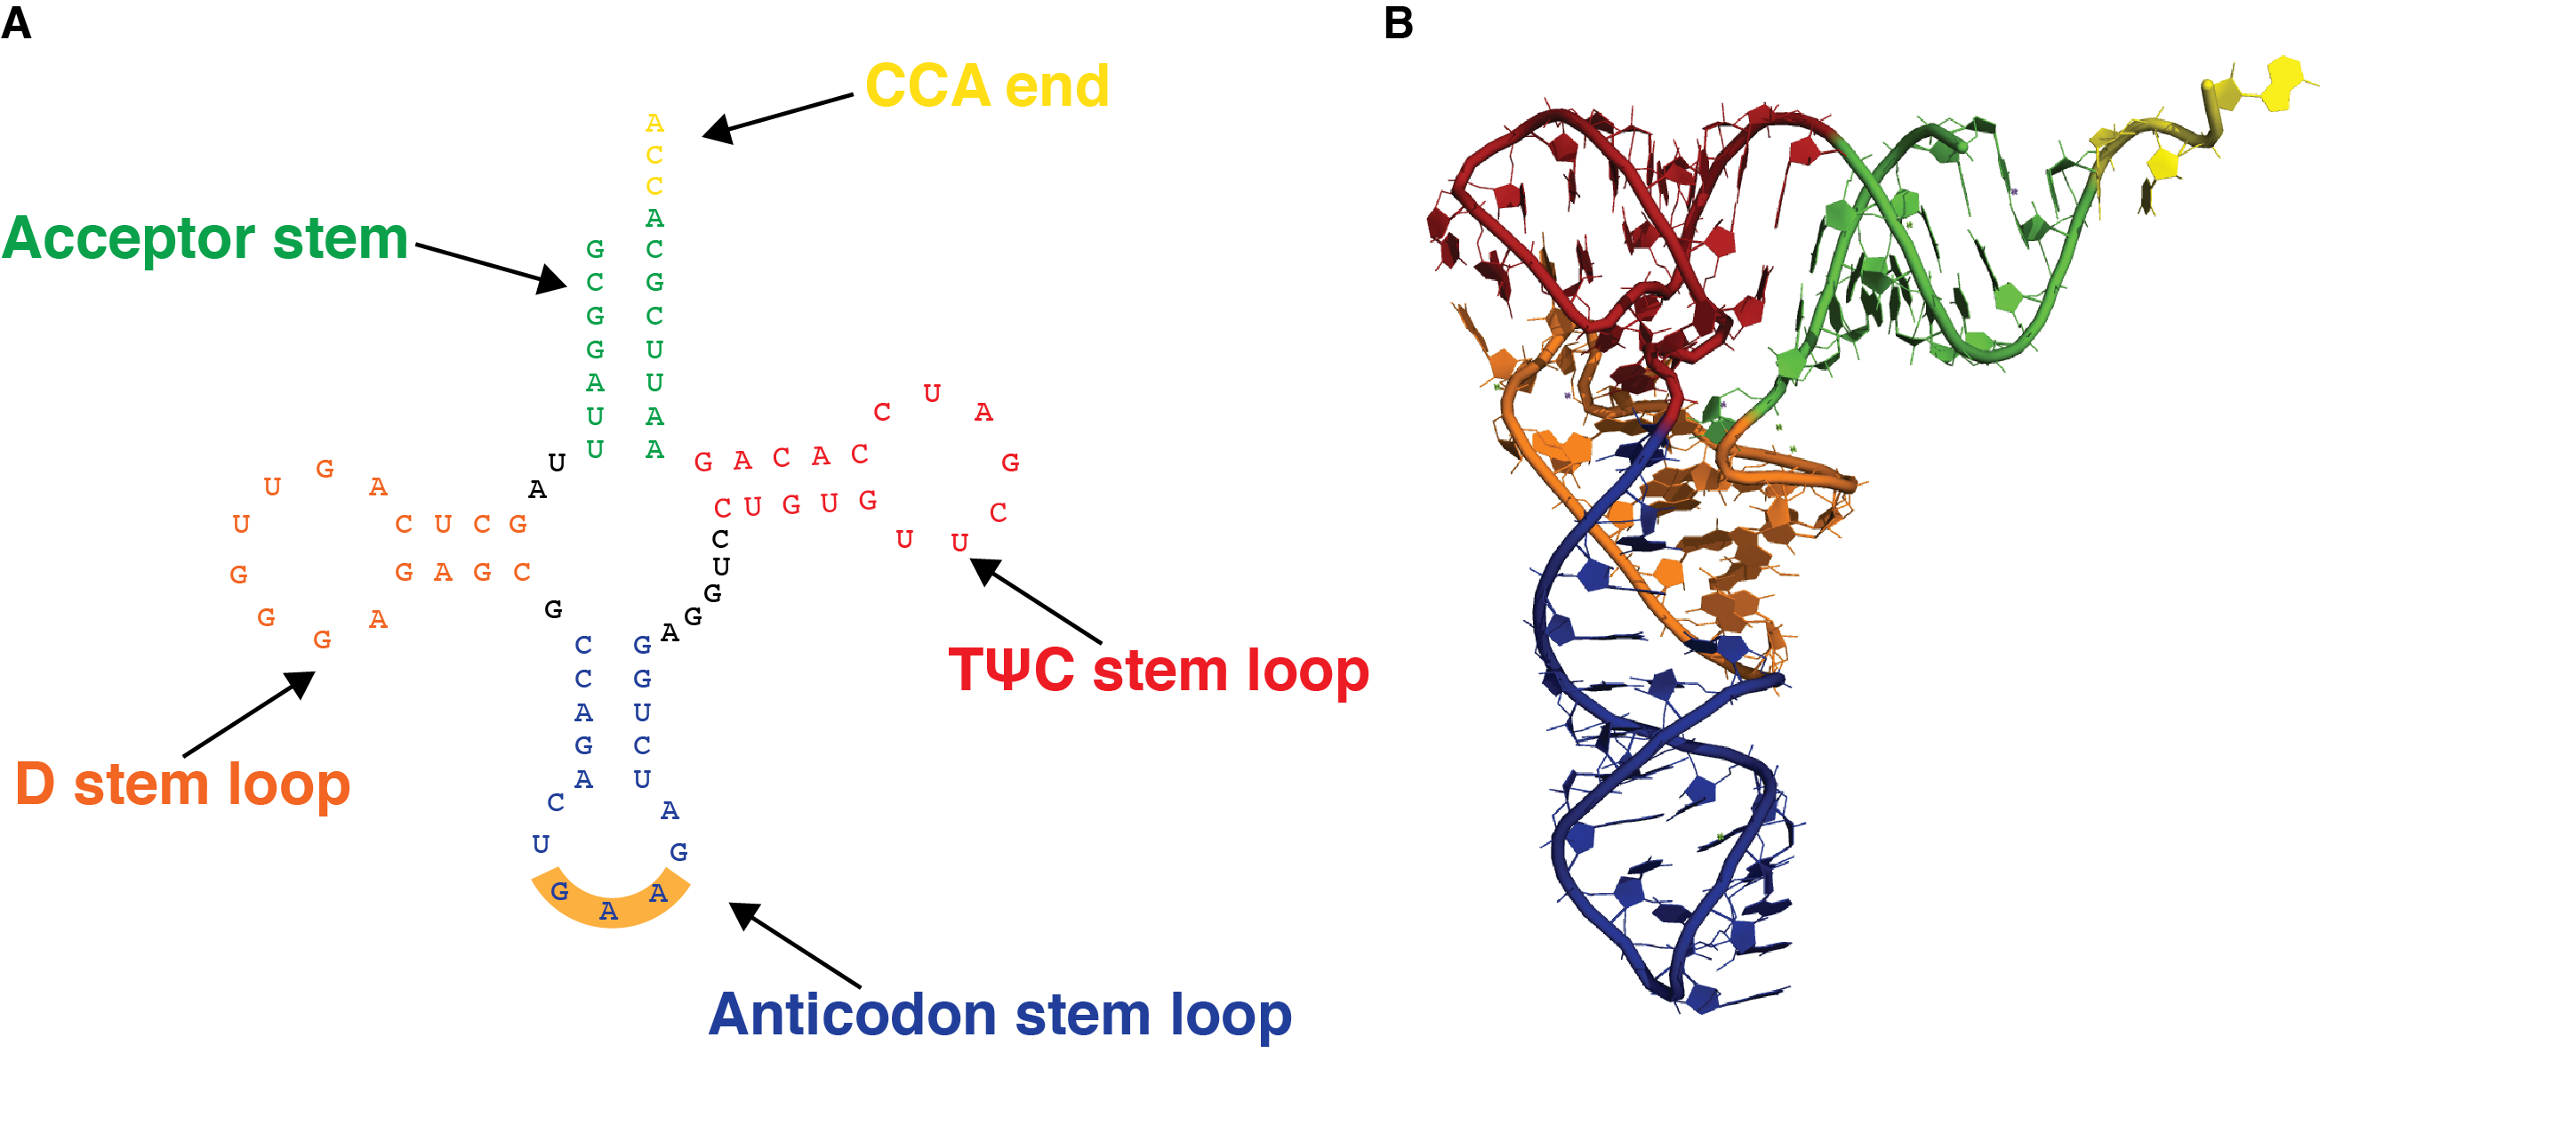
\includegraphics[width=\textwidth]{tRNA_general_structure.png}%
\caption[tRNA structure]{\textbf{tRNA structure}. (A) tRNA transcripts, such as the phenylalanine tRNA shown here, adopt the typical "cloverleaf" secondary, which in turns adopts an L-shaped tertiary structure as shown in (B). The structurally conserved stems and stemloops are indicated in A, color-coded, and their coordinates are reflected in the 3-dimensional structure in B (PDB 1EHZ).
}
%\textbf{\caption{tRNA biogenesis}} 
\label{tRNAstructure}%
\end{figure}

\section{tRNA and disease} 
talk about javier's papers, schimmel and dreyfuss review

\section{tRNA biogenesis}\label{biogenesis}
tRNA genes are transcribed by POLR3 that uses promoters internal to the DNA sequence of the tRNA gene (tDNA), resulting in a primary transcript with a 5' triphosphate. In humans, a minority of tRNA transcripts harbor introns (see section ref{introns}). A dedicated tRNA splicing complex composed of core and accessory proteins carries out tRNA splicing \cite{trotta1999trna,Paushkin:2004wl,Weitzer:2007hda, Popow:2011ffa,Popow:2014ita}. Pre-tRNAs comprise the mature tRNA sequence, and 5' leader and 3' trailer extensions, which are trimmed in a coordinated manner by endonucleases and other processing factors. The \gls{rnp} complex RNase P removes the 5' leaders, leaving a 5' monophospahte, and ELAC2, the human homolog of tRNase Z trims the 3' trailer, leaving a 3' \gls{hydroxyl}. Next, the universally conserved 3' terminal CCA tail is added by the tRNA nucleotidyl transferase 1 (TRNT1), and acts as the acceptor of the amino acid. tRNAs are further modified by chemical nucleotide modifications (\ref{modifications}), exported from the nucleus to the cytoplasm where they can undergo further modifcations, are aminoacylated with their cognate amino acid by aminoacyl tRNA synthetases, and are finally presented to the ribosome by translation factors to participate in protein synthesis (\textbf{Fig. \ref{biogenesis}})\cite{Phizicky:2010jf,Hopper:2010ho,Hopper:2013dl}.

Although these processes allow for multiple levels of regulation, variation in tRNA expression across tissues or between normal and pathologic conditions has not been studied extensively, mainly for two reasons. First, until recently there was the assumption that their essentiality obviated a need for any specialized transcriptional or post-transcriptional control. Second, the lack of an extensively curated and experimentally validated tRNA profile prevented quantitative and systematic studies. Nevertheless, it is now clear that the expression of tRNAs can be dynamic and can indeed exhibit tissue specificity \cite{Dittmar:2006du,Gingold:2014iz}. Importantly, abnormal tRNA expression levels have been correlated and causally associated with pathologic conditions, such as cancer \cite{Gingold:2014iz,Goodarzi:2016gd}.
\newpage

\begin{figure}[!ht]%
\centering
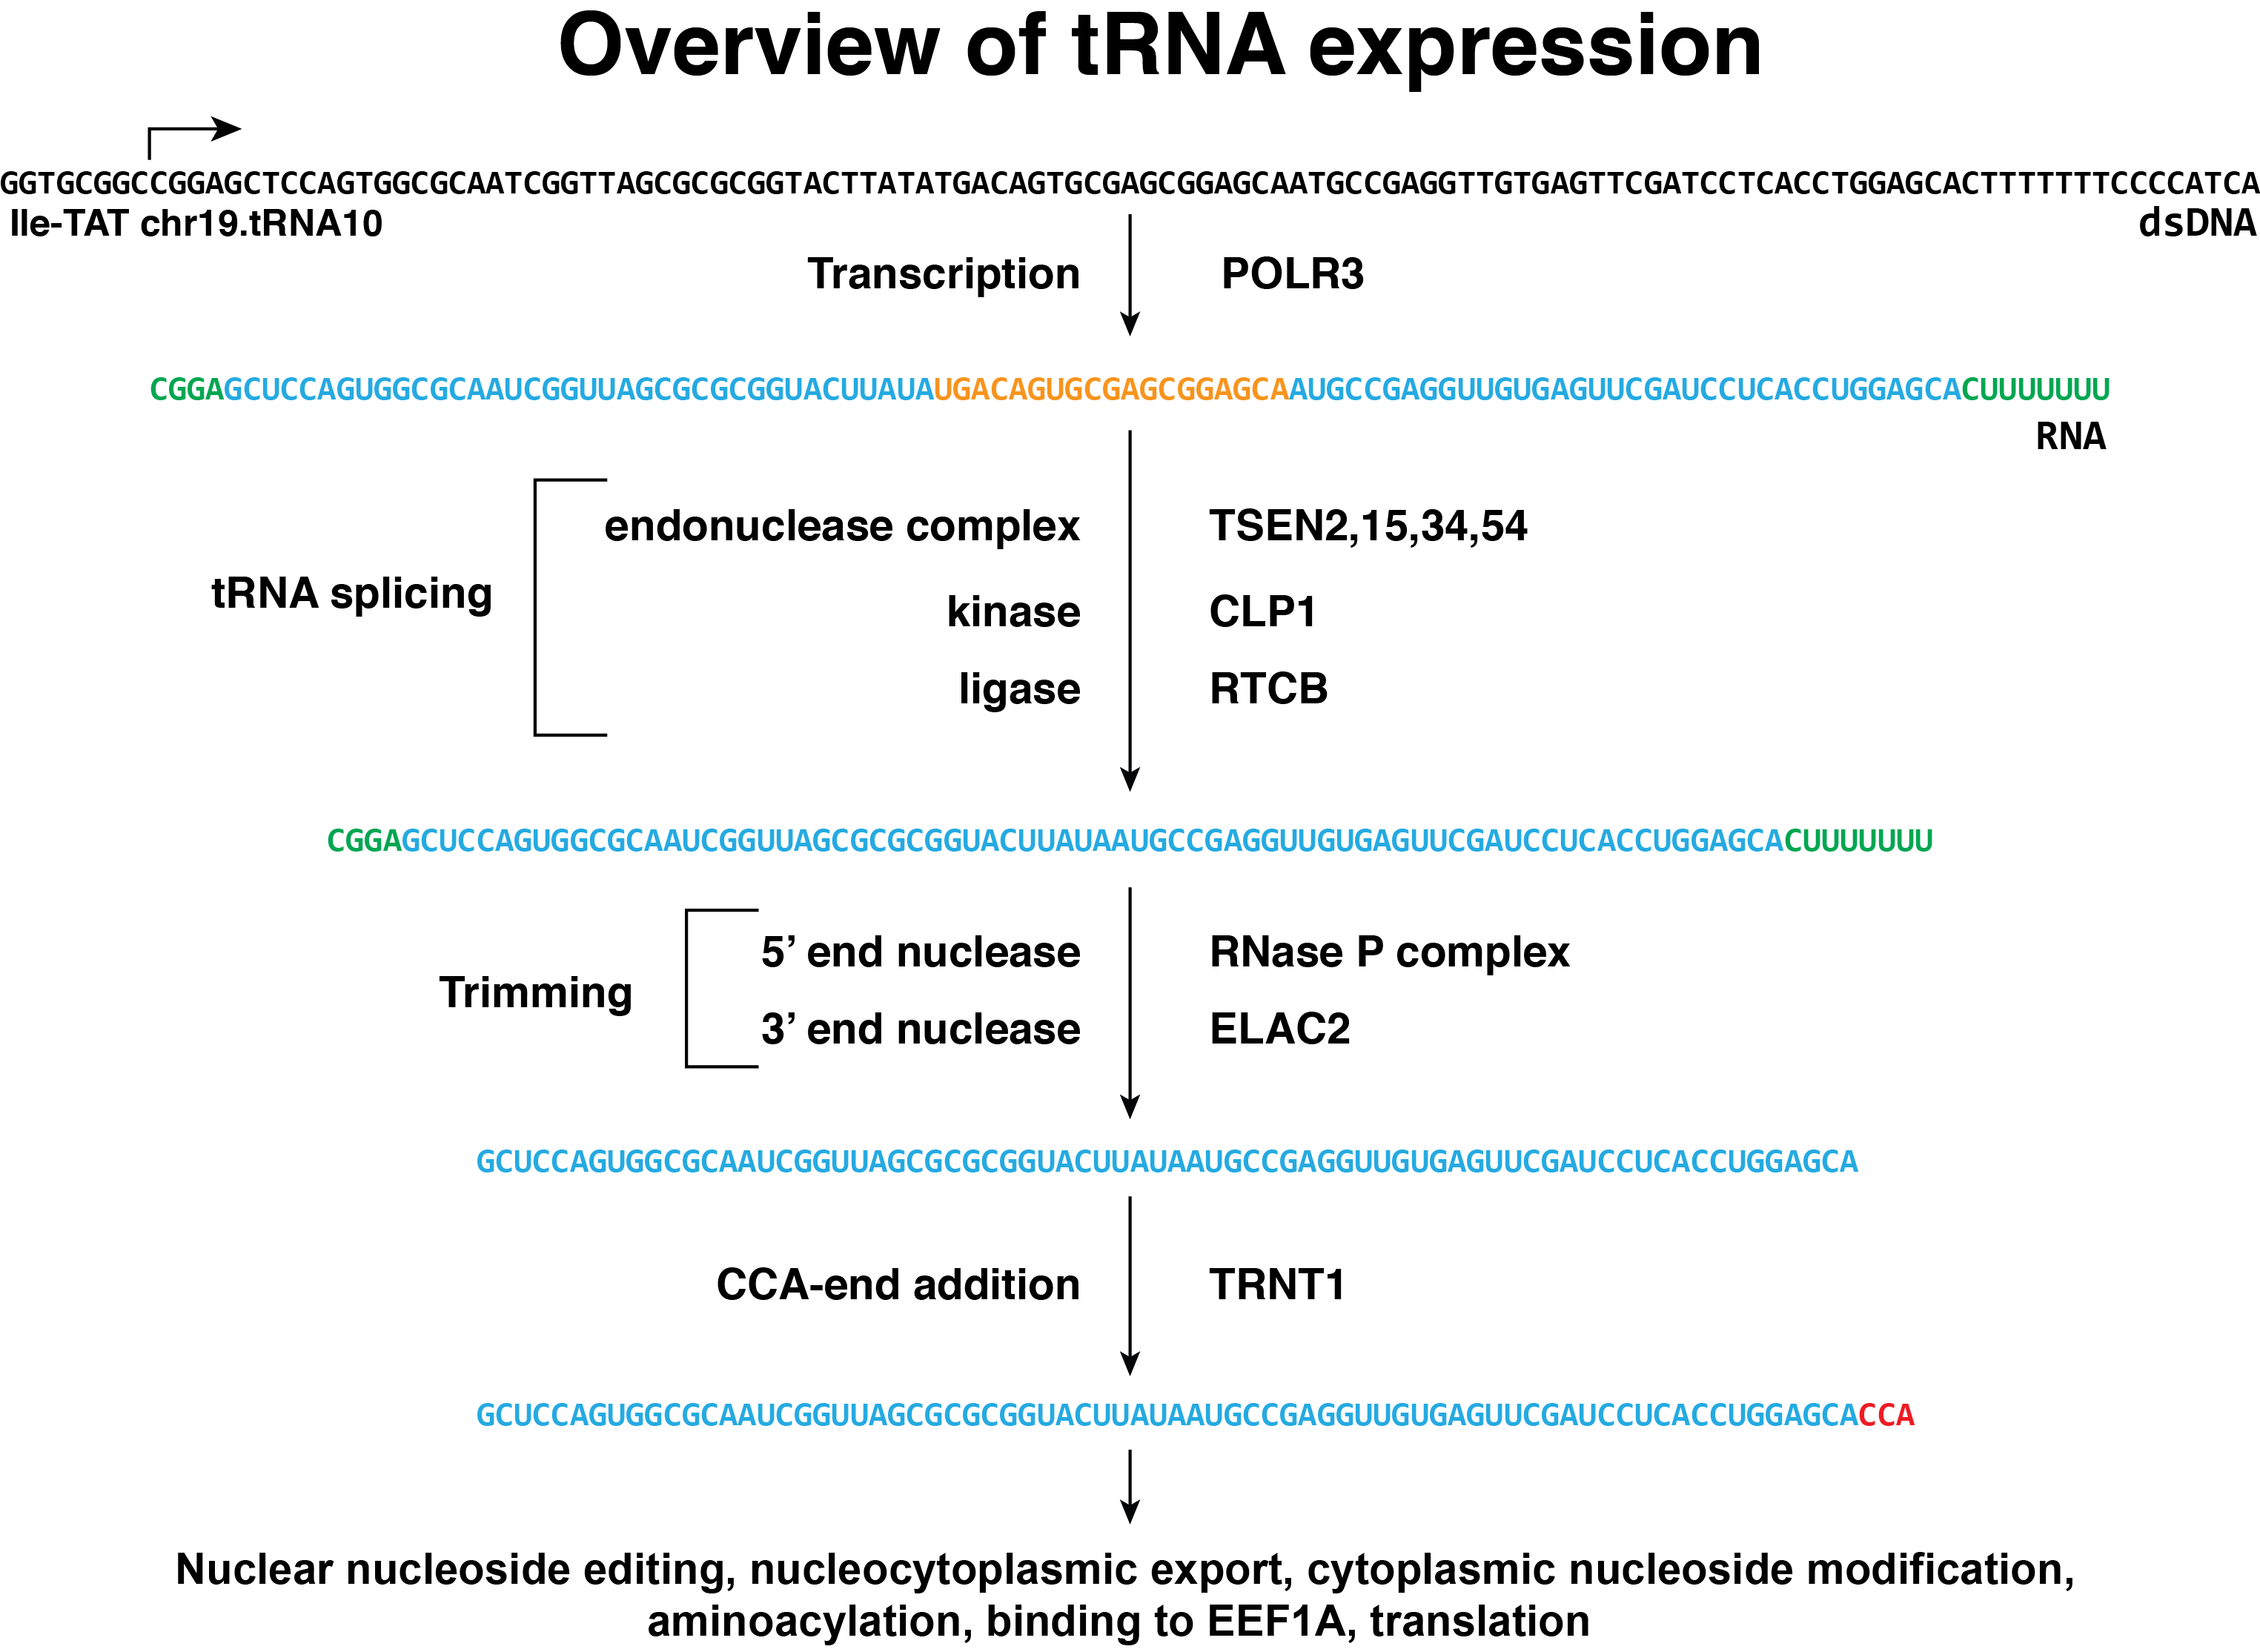
\includegraphics[width=\textwidth]{biogenesis2.png}%
\caption[tRNA biogensis]{\textbf{Overview of tRNA biogenesis and processing.} tRNAs are transcribed by POLR3. If present, tRNA introns are removed by the tRNA splicing complex, and mature halves are ligated by the tRNA ligase (RTCB). Pre-tRNA leaders are trimmed by the RNase P complex, and 3' trailer by ELAC2. The 3' terminal CCA tail is added by TRNT1. tRNAs are further modified by nucleoside editing in the nucleus and the cytoplasm, are aminoacylated by cognate tRNA synthetases and are presented to the ribosome by translation factors.}
%\textbf{\caption{tRNA biogenesis}} 
\label{biogenesis}%
\end{figure}

\section{tRNA sequencing}
This complex biogenesis and processing pathway adds multiple layers of difficulty to the analysis of tRNAs. Obtaining  data for tRNAs is hindered by multiple obstacles:

\begin{enumerate}[i)]
\item sequencing of tRNAs is technically arduous due to their relatively small size, and their stable structure that impedes enzymes used in cDNA library preparations, such as RNA ligases and \gls{rt}
\item numerous (>100) tRNA pseudogenes are interspersed in the human genome \cite{Lowe:1997uc,Chan:2009dz}
\item all tRNAs undergo extensive post-transcriptional processing (see \ref{biogenesis}, while some involve extra processing steps (intron removal, addition of a 5’ guanosine to all histidine tRNAs \cite{Gu:2003jj})
\item tRNAs are subjected to extensive chemical modifications on numerous nucleosides, which lead to mismatches upon the reverse transcription step of the RNA cloning protocols \cite{Jackman:2012ki,Lee:2013cg}. Some modifications are universally conserved and required for proper tRNA function (e.g. adenosine to inosine deamination at the wobble position of the anticodon and methylation of adenosine in the T$\Psi$C loop) \cite{Jackman:2012ki,Gustilo:2008ge}. Since alignment algorithms cannot tolerate multiple mismatches, it is likely that significant numbers of tRNA reads are excluded even if non-default mapping parameters are used.
\item \gls{isoacceptors} share a large degree of sequence similarity that makes the distinction between alternative isoacceptors and editing products equivocal. 
\item eukaryotic cells harbor two distinct populations of tRNAs, nuclear and mitochondrial, whose length, structure, genomic organization, and processing differ considerably, and thus call for customized annotation procedures.
\end{enumerate}

Owing to all these hurdles, the normal genetic makeup and variation of the tRNA population in human cells has not been probed adequately with \gls{rnaseq} tools. Instead information about tRNA sequences and genes comes from bioinformatic predictions \cite{Lowe:1997uc,Chan:2009dz}. Such approaches take into account base-pair covariation, secondary structure predictions of the classical cloverleaf fold of tRNAs, and the tRNA promoter and termination architecture, and scan the human genome in order to identify sequences that are likely to obtain the typical tRNA structure. These analyses have resulted in the most comprehensive standard for whole-genome, predictive annotation of tRNAs so far, and the sequences they have predicted have been used extensively as bona fide tRNAs.

\section{Previous efforts for genome-wide tRNA annotation}

Even though no direct and rigorous experimental validation of tRNA sequences has been carried out, there has been indirect experimental evidence for tRNA expression:

\begin{enumerate}[i)]
\item ChIP-seq studies focusing on the occupancy of genomic locations by POLR3 and/or its transcription factors \cite{Moqtaderi:2010hc,Oler:2010fb,Kutter:2011ff}
\item tRNA microarrays that use the predicted tRNA sequences as the reference for the creation of array probes \cite{Dittmar:2004fb}
\end{enumerate}

These methods, though, have several limitations. ChIP-seq, for example, uses chromatin occupancy as a proxy for productive RNA synthesis. Conversely, tRNA microarrays have limited sensitivity and specificity thresholds due to off-target hybridization that is potentiated by nucleoside modifications21, while their dynamic range is considerably narrower than RNA-seq. Finally, neither method is appropriately equipped to determine definitively pre-tRNAs or their transcription start and termination sites. This is an important limitation, as pre-tRNA fragments have been associated with neurodegenerative diseases \cite{Hanada:2013bk, Weitzer:2014bi, Karaca:2014em}. 
	
\section{Small RNA sequencing protocol}
In order to obtain RNA-seq reads, I decided to first apply the well established protocol for sequencing small RNAs, established in the Tuschl lab \cite{Hafner:2012eaa} (\textbf{Fig. \ref{sRNA}}). The experimental procedure takes advantage of the 5' monophosphate (p) and 3' OH groups present in small RNAs, such as \glspl{miRNA}, in order to enrich for such RNA species over other abundant RNA molecules. The use of a truncated and mutated RNA ligase (T4 Rnl2(1-249)K227Q) that requires 5' preadenylated adapter (App-(5')-adapter) prevents on one hand the formation of secondary, circularized byproducts, and allows on the other for exclusive ligation at the 3' end of the target RNA. Rnl1 is used to ligate an adapter with a different sequence at the 5' end, by activating the 5' monophosphate of the small RNA. cDNA is obtained by RT and amplified at non-saturated levels by PCR. The derived small RNA cDNA library is submitted to high-throughput on Illumina instruments using sequencing primer sites present in the adapter sequences. The different sequences of the 3' and 5' adapters preserves the strandedness of the original RNA sequence, enhancing ncRNA discovery and curation. Adding short (5-nt) barcode sequences at the 3' adapter also allows for pooling of several multiplexed samples, reducing costs, processing time, and batch variability. 

\begin{figure}[!ht]%
\centering
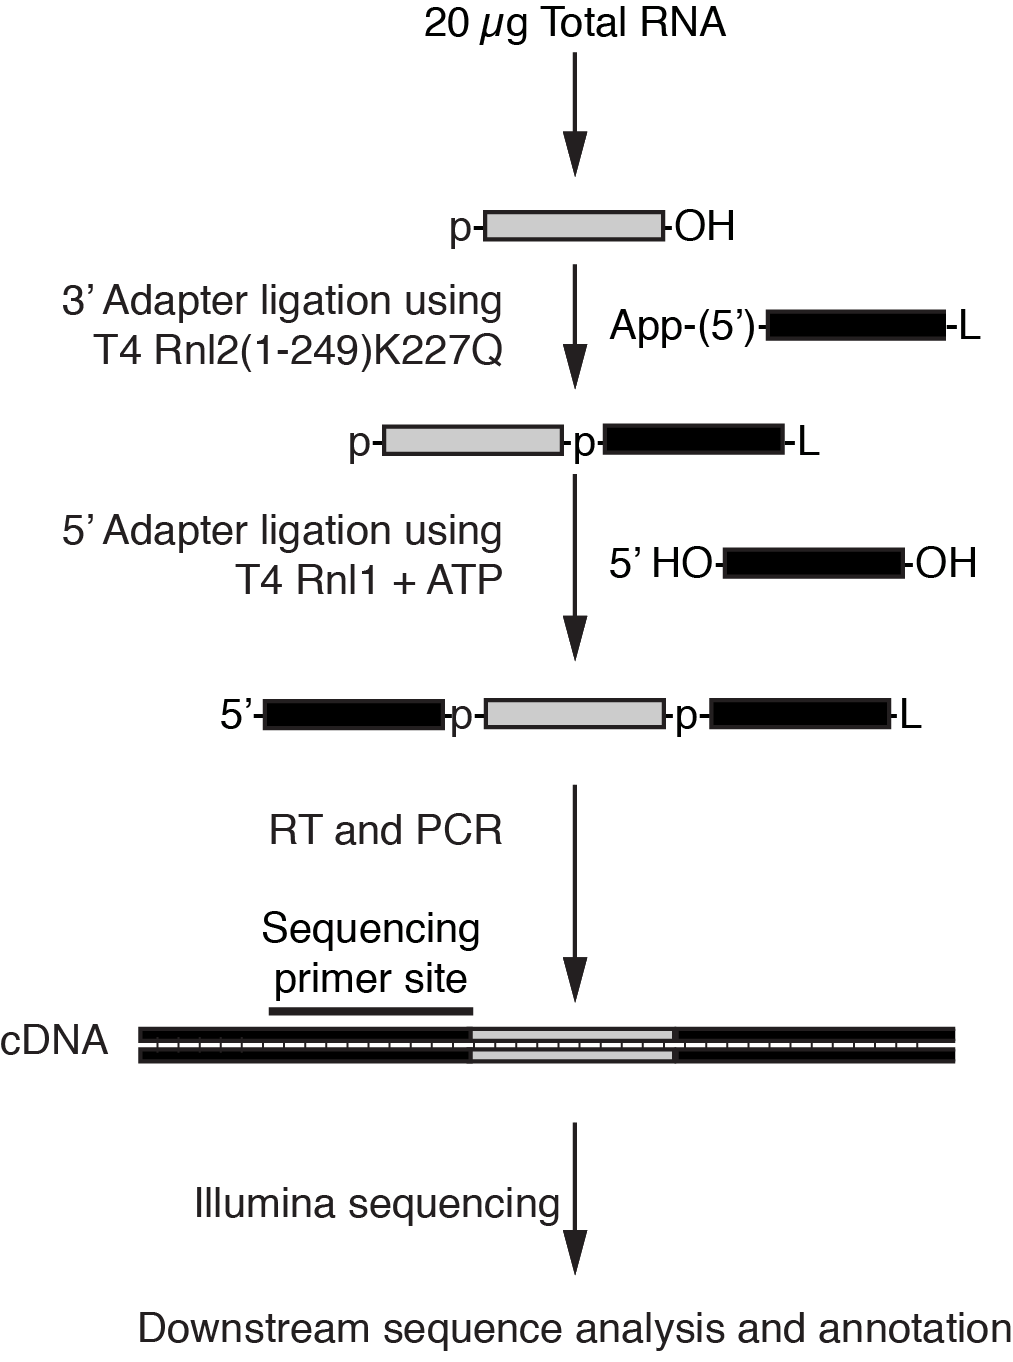
\includegraphics[width=3.5in]{sRNA.png}%
\caption[Small RNA sequencing protocol]{\textbf{Small RNA sequencing protocol}. Schematic overview of the conventional small RNA sequencing protocol, as it has been described previously \cite{Hafner:2012eaa}} 
\centering
\label{sRNA}%
\end{figure}

Even though the utility of this protocol has been documented for the discovery and quantification of miRNAs, it was reasonable to apply towards tRNA sequencing because:
\begin{enumerate}
\item tRNAs, which are on average 75 \glspl{nt} long, are closer in length than most other highly abundant ncRNAs (typically longer than 150 nts) 
\item mature tRNAs and miRNAs both have a 5' monophosphate and 3' OH, which are employed at different steps of library preparation
\end{enumerate}

The application of this protocol for tRNA sequencing, though, resulted in \gls{rnaseq} datasets with only \~2\% tRNA content, with an average length of 59 nts (\textbf{Table. \ref{abysmal}}). These suggested that tRNAs were refractory to the small RNA sequencing protocol, and necessitated the development of a novel sequencing protocol. 

\begin{table}[!ht]
\begin{center}
\tabulinesep=1.2mm
\begin{tabu}{ | l | r | r |}
	\hline
    RNA type & \% Total reads & Mean length (nt) \\ \hline
	rRNA & 35.8\% & 60.5 \\ \hline
	no match  & 24.1\% & 76.2 \\ \hline
	no annotation & 17.8\% & 64.2 \\ \hline
	snRNA/snoRNA & 15.1\% & 62.5 \\ \hline
	repeat & 3.8\% & 59.1 \\ \hline
	tRNA & 2.0\% & 59.1 \\ \hline
	miscRNA & 1.3\% & 63.1 \\ \hline
	miRNA & 0.1\% & 22.2 \\
	\hline
\end{tabu}
\end{center}
\caption[RNA types recovered by small RNA sequencing protocol]{\textbf{RNA types recovered by small RNA sequencing protocol.} Percentage of reads mapped to indicated ncRNA type over total depth of library, and mean length of reads mapped to RNAs of each type are shown. snRNA: small nuclear RNA; snoRNA: small nucleolar RNA; repeat: repetitive DNA sequence; miscRNA: all other ncRNAs.	}\label{abysmal}
\end{table}

\chapter{Hydro-tRNAseq}

\section{Experimental innovation}
In order to overcome the problems associated with tRNA sequencing, I tried to identify the minimal number of simplest steps that could tackle the maximal number of problems. Thus, I isolated 60-100 nt-sized total RNA from \gls{hek293} cells, comprising both pre- and mature tRNAs, but being devoid of most other abundant RNAs and short tRNA turnover products \cite{Lee:2009fb}. Full-length tRNAs have thermodynamically stable secondary and tertiary structures and are heavily modified by RNA editing, all of which compromise RT and RNAseq analysis. To overcome these problems, I implemented a limited alkaline hydrolysis step. I reasoned that hydrolysis would generate shorter RNA fragments less prone to adopt stable structures, and would also reduce the number of per sequenced fragment. 

The value of the latter effect becomes apparent if one performs the following thought experiment. Let us assume that the probability of an RT "problem" (stall, drop or misincorporation) is the same for all modifications (e.g. $p$). The compound probability of RT stalling, dropping or misincorporating a nucleoside in a given sequence is given by the product of any of these events happening at a given modified position is 
\begin{equation}
P = p^n
\end{equation}
where  $n = \text{number of modified nucleosides affecting RT}$. 
Given that full length tRNAs are longer than the hydrolysis-derived fragments, and modifications are usually concentrated in the loops of the tRNA (see (\textbf{Fig. \ref{tRNAstructure}} and \textbf{Fig. \ref{paper7a}}), then 
\begin{equation}
n_{full-length} \geq n_{fragment} 
\end{equation}
and therefore: 
\begin{equation}
P_{full-length} \geq P_{fragment}
\end{equation}
and the probability of sequencing through an RNA fragment $(1-p)$:
\begin{equation}
1-P_{full-length} \leq 1-P_{fragment}
\end{equation}

\begin{figure}[!h]%
\centering
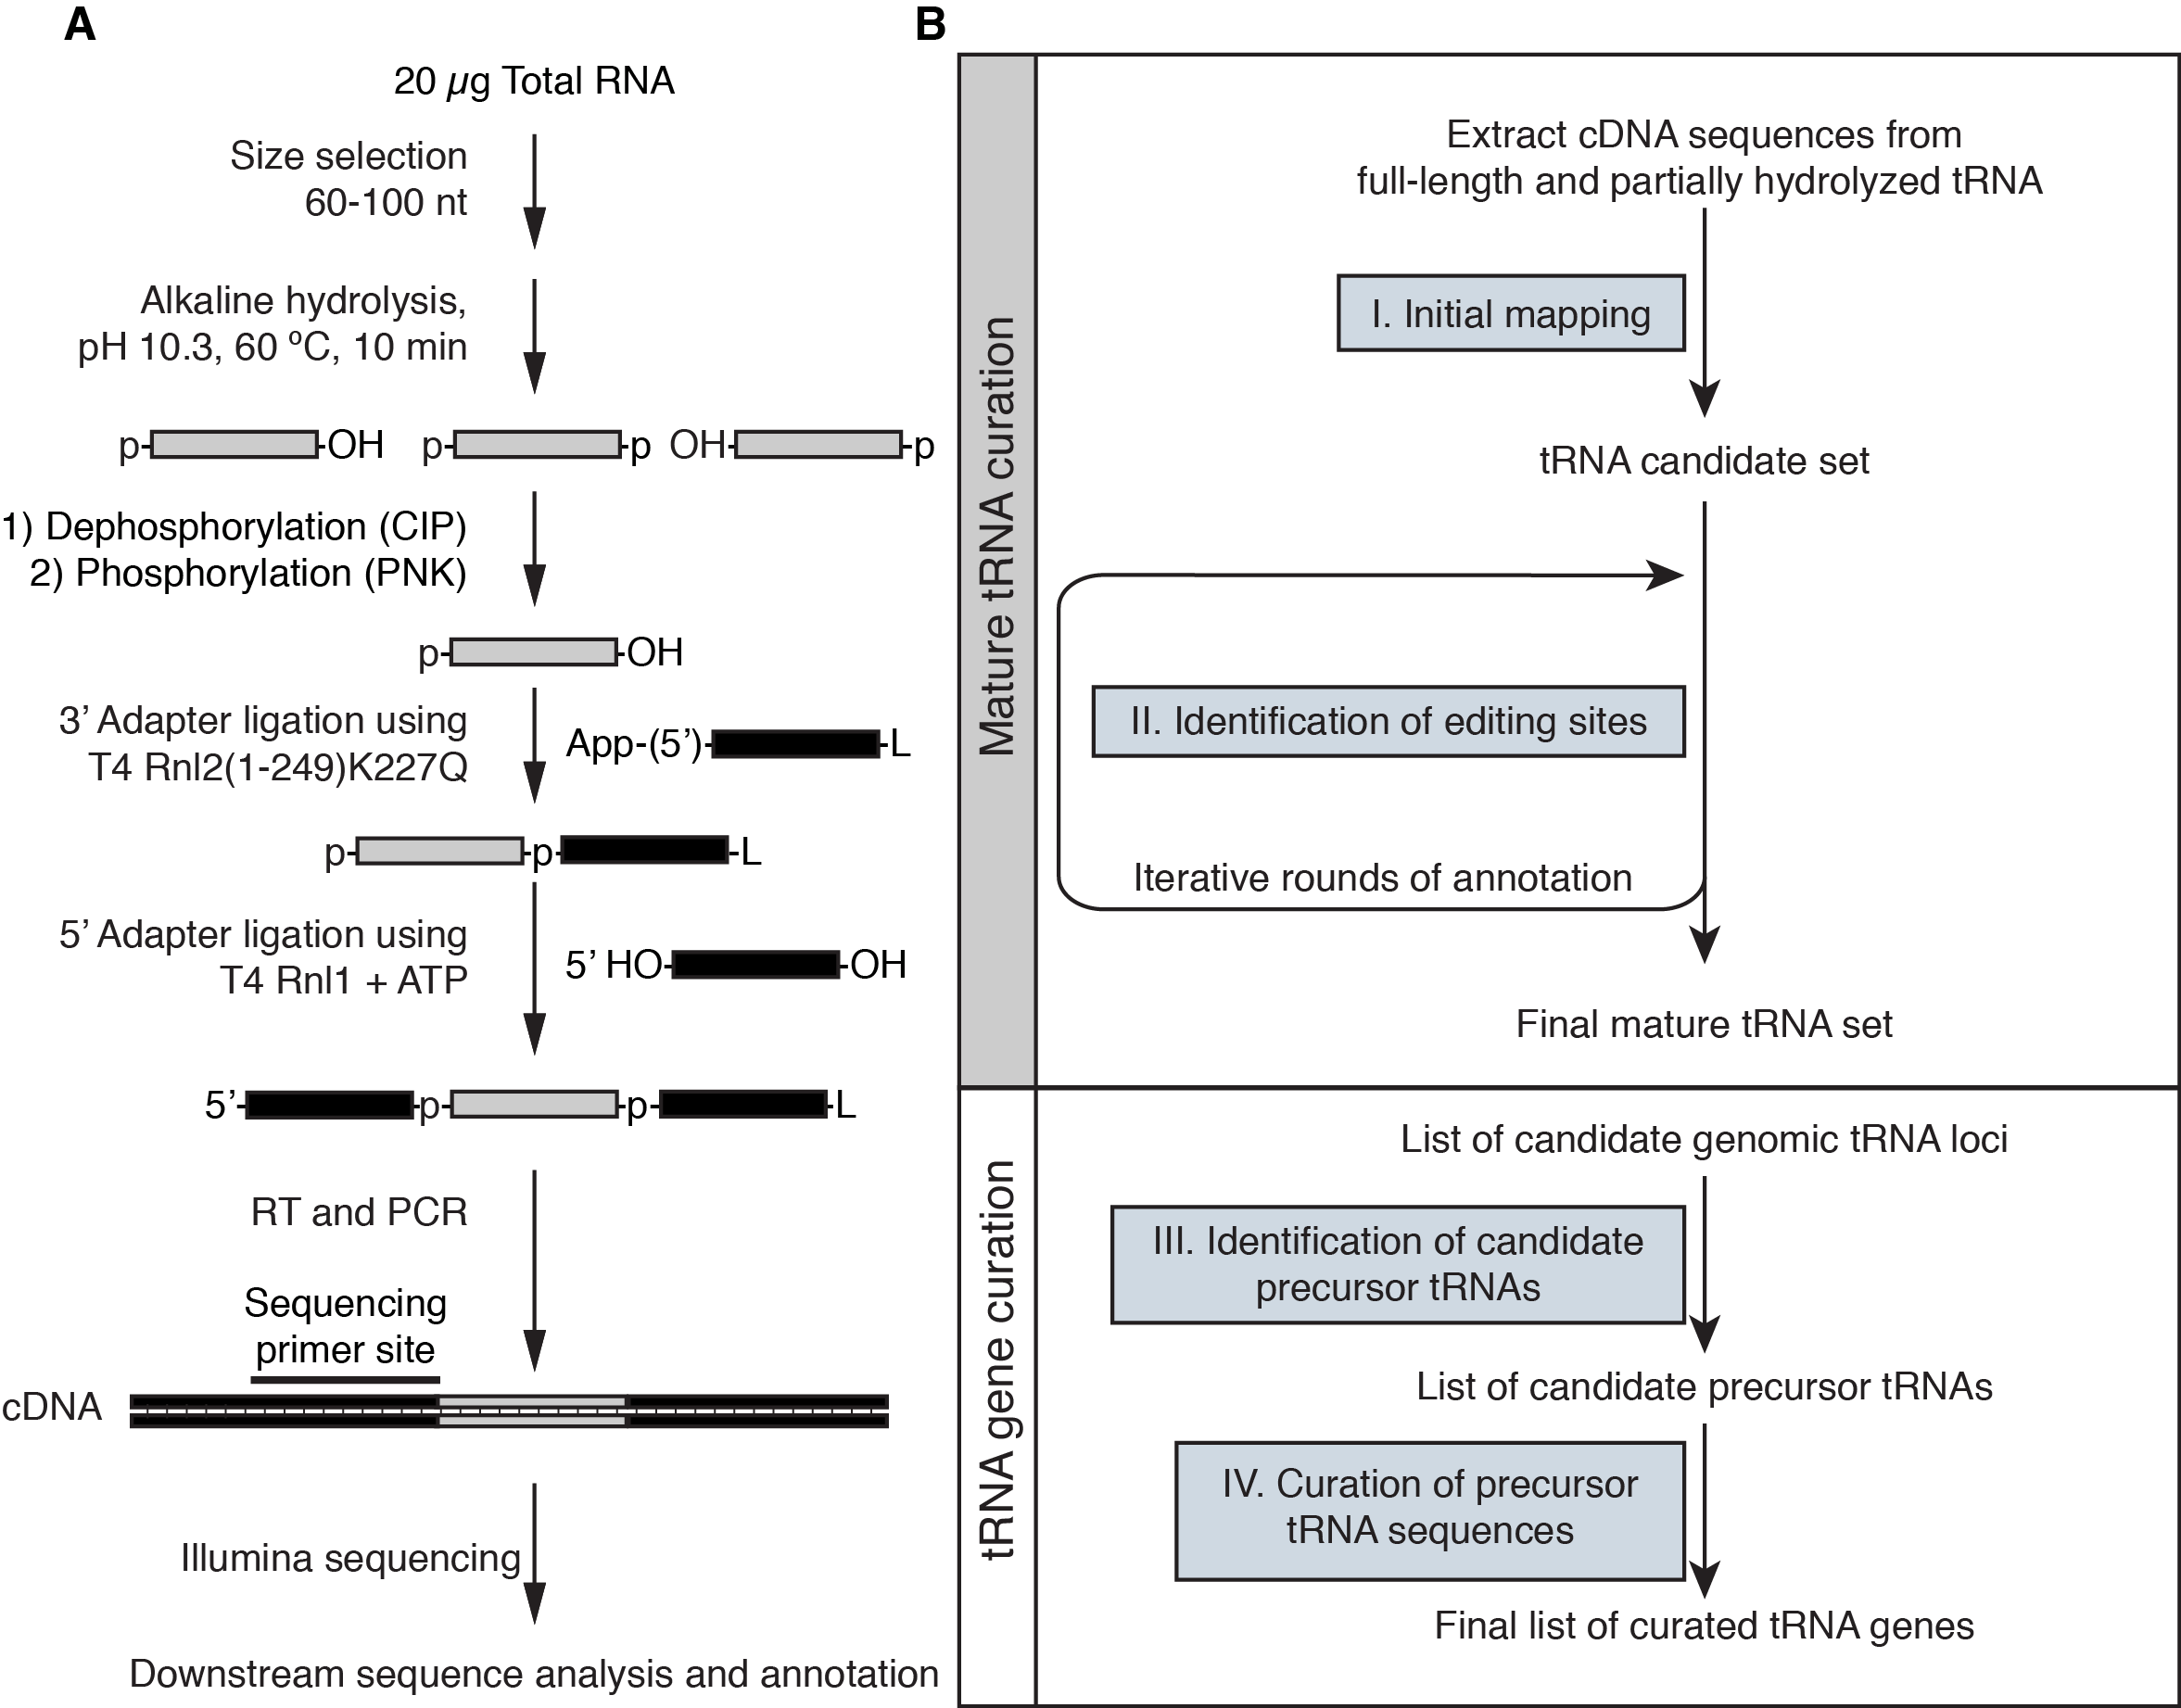
\includegraphics[width=\textwidth]{paper1.png}%
\caption[hydro-tRNAseq experimental and bioinformatic pipeline]{\textbf{Hydro-tRNAseq experimental and bioinformatic pipeline for tRNA annotation and reference transcript curation by hydro-tRNAseq.}(A) tRNAs and pre-tRNAs were size-selected from HEK293 total RNA and subjected to limited alkaline hydrolysis, followed by dephosphorylation, rephosphorylation and conventional small RNA sequencing as described previously (Hafner et al., 2012). (B) An iterative mapping and annotation protocol was used to first annotate and curate fully processed and nucleotide-modified mature tRNAs. Leftover reads that spanned the mature-precursor junctions were used to identify transcribed tRNA genes.}
\centering
\label{paper1}%
\end{figure}

In addition to increasing read-through by RT, the reduced frequency of modified nucleosides per sequenced fragment, also improves mapping efforts by reducing the number of mismatches per sequenced read. Furthermore, basic conditions also cleave the aminoacyl-tRNA bond, freeing the 3’ terminal hydroxyl group required for 3’ adapter ligation during RNA cDNA library preparation. Thus, I anticipated that collectively these effects would yield RNA sequences more amenable to small RNA cDNA library preparation and deep sequencing than the refractory tRNAs. Indeed this approach increased the tRNA read content to >40\% in our deepest dataset (\textbf{Table \ref{tableS1}}). We named this procedure hydro-tRNAseq (\textbf{Fig. \ref{paper1}A}).

Encouraged by the preliminary performance of the protocol, I set out to obtain a curated list of human nuclear and mitochondrial tRNAs, their genomic loci,  and their processing intermediates. However, such an effort required a custom-made computational analysis pipeline.

\begin{table}[h!]
  \begin{adjustbox}{max width = \textwidth}
  \def\arraystretch{1.5}
  \tabulinesep=1.2mm  

  \begin{tabular}{|l|l|l|l|l|l|l|l|l|l|l|l}
\hline
           Type &   D0 counts &   D1 counts &  D2 counts &        Total & \multicolumn{1}{m{2.5cm}|}{\% total starting}  & \multicolumn{1}{m{2cm}|}{\% over mapped reads}  & \multicolumn{1}{m{2.5cm}|}{\% D0/ total D0} & \multicolumn{1}{m{2cm}|}{D0/total (per type)} & D1/total & D2/total \\
\hline
           tRNA &  41,880,208 &   9,444,737 &  2,814,103 &   54,139,048 &               44\% &                  47\% &            47\% &                 77\% &      17\% &       5\% \\
           rRNA &  18,825,243 &   4,317,680 &  1,222,652 &   24,365,575 &               20\% &                  21\% &            21\% &                 77\% &      18\% &       5\% \\
        mt tRNA &  15,254,805 &   2,976,430 &    736,595 &   18,967,830 &               15\% &                  17\% &            17\% &                 80\% &      16\% &       4\% \\
         snoRNA &   8,126,590 &   1,635,120 &    388,833 &   10,150,543 &                8\% &                   9\% &             9\% &                 80\% &      16\% &       4\% \\
           mRNA &     951,538 &     231,248 &     89,536 &    1,272,322 &                1\% &                   1\% &             1\% &                 75\% &      18\% &       7\% \\
      mRNA gene &     828,458 &     229,342 &    150,541 &    1,208,341 &                1\% &                   1\% &             1\% &                 69\% &      19\% &      12\% \\
          snRNA &     773,703 &     169,800 &     43,861 &      987,364 &                1\% &                   1\% &             1\% &                 78\% &      17\% &       4\% \\
      pre-tRNA &     529,077 &     247,304 &    146,557 &      922,938 &                1\% &                   1\% &             1\% &                 57\% &      27\% &      16\% \\
         genome &     327,950 &     114,402 &    153,951 &      596,303 &                0\% &                   1\% &             0\% &                 55\% &      19\% &      26\% \\
        mt rRNA &     363,913 &      86,271 &     24,813 &      474,997 &                0\% &                   0\% &             0\% &                 77\% &      18\% &       5\% \\
          scRNA &     339,135 &      91,056 &     27,098 &      457,289 &                0\% &                   0\% &             0\% &                 74\% &      20\% &       6\% \\
         marker &     113,303 &      52,725 &     32,143 &      198,171 &                0\% &                   0\% &             0\% &                 57\% &      27\% &      16\% \\
      rRNA prec &     106,373 &      49,811 &     12,589 &      168,773 &                0\% &                   0\% &             0\% &                 63\% &      30\% &       7\% \\
      bacterial &      31,724 &      38,555 &     52,354 &      122,633 &                0\% &                   0\% &             0\% &                 26\% &      31\% &      43\% \\
        mt mRNA &      47,466 &      12,816 &      4,887 &       65,169 &                0\% &                   0\% &             0\% &                 73\% &      20\% &       7\% \\
   lincRNA gene &      35,934 &      10,686 &      9,516 &       56,136 &                0\% &                   0\% &             0\% &                 64\% &      19\% &      17\% \\
      mt genome &      17,990 &      14,749 &     20,379 &       53,118 &                0\% &                   0\% &             0\% &                 34\% &      28\% &      38\% \\
          miRNA &       5,425 &       7,443 &     38,348 &       51,216 &                0\% &                   0\% &             0\% &                 11\% &      15\% &      75\% \\
        lincRNA &      26,713 &       6,474 &      1,460 &       34,647 &                0\% &                   0\% &             0\% &                 77\% &      19\% &       4\% \\
    snoRNA prec &      22,776 &       6,544 &      2,774 &       32,094 &                0\% &                   0\% &             0\% &                 71\% &      20\% &       9\% \\
        plasmid &       9,461 &       3,193 &      1,896 &       14,550 &                0\% &                   0\% &             0\% &                 65\% &      22\% &      13\% \\
         scaRNA &      10,065 &       2,184 &        526 &       12,775 &                0\% &                   0\% &             0\% &                 79\% &      17\% &       4\% \\
     snRNA prec &       7,207 &       2,076 &      1,934 &       11,217 &                0\% &                   0\% &             0\% &                 64\% &      19\% &      17\% \\
          piRNA &       1,227 &         866 &      1,283 &        3,376 &                0\% &                   0\% &             0\% &                 36\% &      26\% &      38\% \\
     scRNA prec &         173 &          43 &        132 &          348 &                0\% &                   0\% &             0\% &                 50\% &      12\% &      38\% \\
        adapter &           0 &           0 &        160 &          160 &                0\% &                   0\% &             0\% &                  0\% &       0\% &     100\% \\
 doubtful miRNA &         101 &          42 &         14 &          157 &                0\% &                   0\% &             0\% &                 64\% &      27\% &       9\% \\
        mirtron &          24 &           5 &          1 &           30 &                0\% &                   0\% &             0\% &                 80\% &      17\% &       3\% \\
    scaRNA prec &          10 &           8 &          1 &           19 &                0\% &                   0\% &             0\% &                 53\% &      42\% &       5\% \\
       std cali &           0 &           0 &          1 &            1 &                0\% &                   0\% &             0\% &                  0\% &       0\% &     100\% \\ \hline
         total  &  88,636,592 &  19,751,610 &  5,978,938 &  114,367,140 &               93\% &                 100\% &           100\% &                 n/a &      n/a &      n/a \\
\hline
  \end{tabular}
  \end{adjustbox}
\caption[Hydro-tRNAseq reads per RNA type]{\textbf{Hydro-tRNAseq reads per RNA type.} Reads assigned to each RNA type following hierarchical annotation are shown. Reads with no (d0), one (d1) or two (d2) mismatches compared to reference are shown. Hydro-tRNAseq enriches for nuclear (44\%) and mitochondiral (15\%) tRNAs}\label{tableS1}
\end{table}

\section{Bioinformatics analysis pipeline}
\subsection{Hierarchical sequence read mapping}
In parallel with the tRNA annotation procedure, we had to build a bioinfroamtic pipeline for processing the obtained sequence information. To account for the multiple maturation steps between pre- and mature tRNAs, in collaboration with bioinformatician Miguel Brown, we developed an iterative, hierarchical approach for mapping and annotating our sequence reads. 

First we mapped reads to reference tRNA genes for the human genome release hg19 (\url{http://gtrnadb.ucsc.edu/}) using an iterative and hierarchical protocol (\textbf{Fig. \ref{paper1}B}). We started by mapping only to mature tRNAs, which included the 3’ CCA aminoacyl acceptor terminus, and the G\sub{-1} nucleotide added posttranscriptionally to histidine tRNAs \cite{Gu:2003jj, Juhling:2009ip}, but excluded tRNA introns. Starting with two most abundant tRNA transcripts per \gls{isotype}  as indicated after the first mapping round, except for selenocysteine, where only one mature tRNA sequence could be identified, we performed iterative rounds of mapping and manual reference transcript selection, focusing in every step on transcripts that collected more reads with an error distance of 1-2 than 0. If these reads with mismatches could be assigned to other tRNA isoacceptors, these were included in our candidate reference set. Otherwise, we reasoned that the mismatches were the results of nucleotide-modification-induced errors of RT. In those cases, we accounted for the modified nucleoside signatures by introducing a new, edited reference transcript in our set. 

For tRNAs that exhibited multiple positions with high modification rates (>10\% compared to reference), we compiled reference sequences with all possible combinations of modified signatures at all detectably modified positions, aiming to account for the maximum possible number of mapped sequence reads. We ended the curation cycles when there was no observed modified position that exhibited a mismatch frequency greater than or equal to 10\% compared to the reference. By performing this iterative process of curation, we obtained an experimentally validated reference set of mature tRNAs accounting for modified-nucleotide-induced sequence variation upon reverse transcription.

\subsection{tRNA gene annotation}
In order to identify possible tRNA gene loci, we mapped the curated tRNA sequences back to the genome, allowing for gaps to accommodate tRNA introns, as well as up to 7 mismatches to accommodate terminal and internal RNA editing events. By appending 40 nts upstream and downstream of the location of genomic mapping, we obtained a candidate pre-tRNA gene set. We mapped non-annotated residual reads to these candidates to identify 5’ leader- and 3’ trailer-comprising pre-tRNA reads. These reads distinguished actively transcribed tRNA genes from silent ones or pseudogenes.

Leader- and trailer-comprising tRNA genes show higher sequence variation, as evidence by higher information entropy values, across the leader and trailer nucleotides than internal sequences within the mature tRNA suggesting that even short precursor sequences with read coverage are sufficient for the annotation of non-redundant tRNA genes (\textbf{Fig. \ref{supp1}}). At the end of our analysis we accounted for 93\% of the 114,367,140 reads in our deepest library (\textbf{\ref{tableS1}}).

Given the depth of sequencing, we are confident that we accounted for the vast majority of precursor and mature tRNAs. Indeed, \textit{a posteriori} we looked for genomic regions that collected at least 50 overlapping reads throughout their whole length, fell within the 60- to 100-nt size window, and adopted a cloverleaf structure, in an effort to detect any tRNAs that might have been overlooked by our approach or in prior literature. The only sequences that we identified were U1 snRNA \hl{(pseudo)genes (Fig. S2)}, suggesting that our analysis was exhaustive, at least for tRNAs in HEK293 cells. 

\begin{figure}[!ht]%
\centering
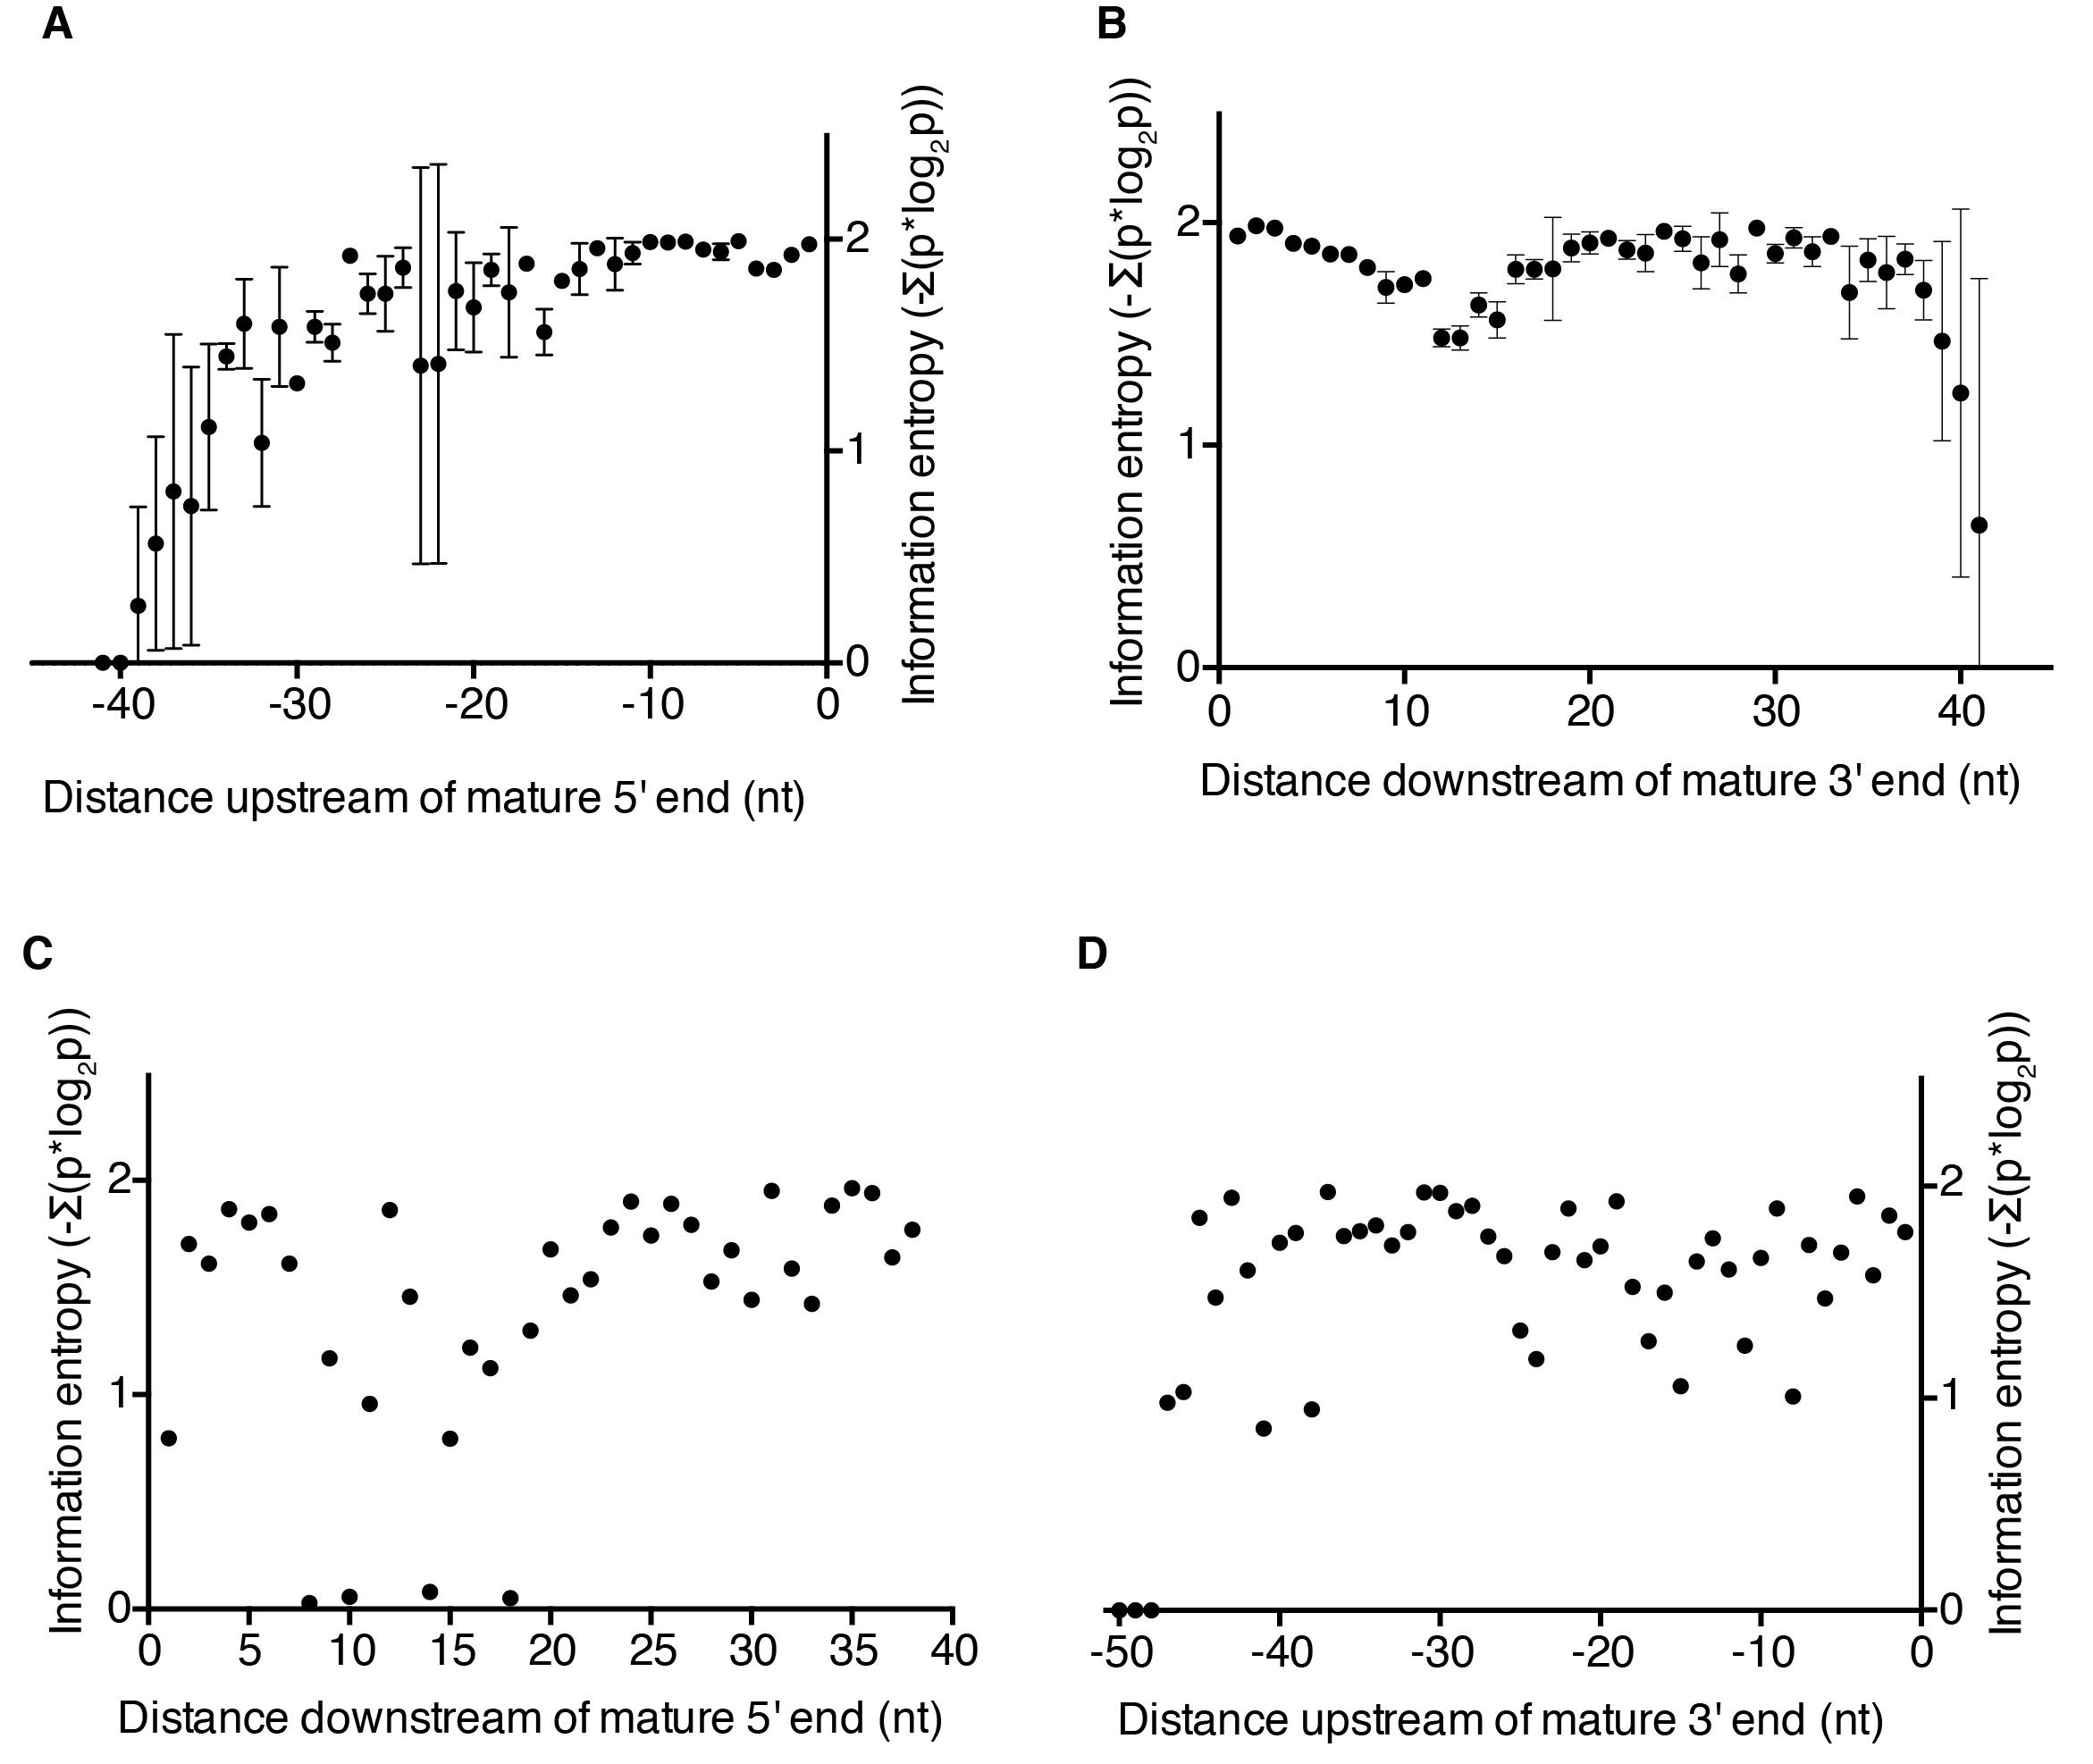
\includegraphics[width=\textwidth]{supp1.png}%
\caption[Information entropy in pre-tRNA segments and mature body]{\textbf{Information entropy in pre-tRNA segments and mature body}
(A,B) Information entropy $H = -\sum_{i=1}^np(i)*log(p(i))$, (where p is the frequency of each nucleotide at a given position, i, and n the total number of transcripts) was calculated using read evidence from hydro-tRNAseq (four replicates) for the 5’ leader and 3’ trailers of all pre-tRNAs with positions centered at the 5’ and 3’ ends of mature tRNAs. (C,D) Same as before, but using the reference sequence of mature tRNAs.}
\centering
\label{supp1}%
\end{figure}

\section{Pipeline outputs}
\subsection{Mature tRNA alignment}

Our pipeline provides individual alignments for every reference transcript included in our curated database. Each alignment is presented in a separate text file (.txt) that can be surveyed without the requirement of any special analysis or display software, as is the case for conventional mRNA-seq datasets. 

\begin{figure}[!ht]%
\centering
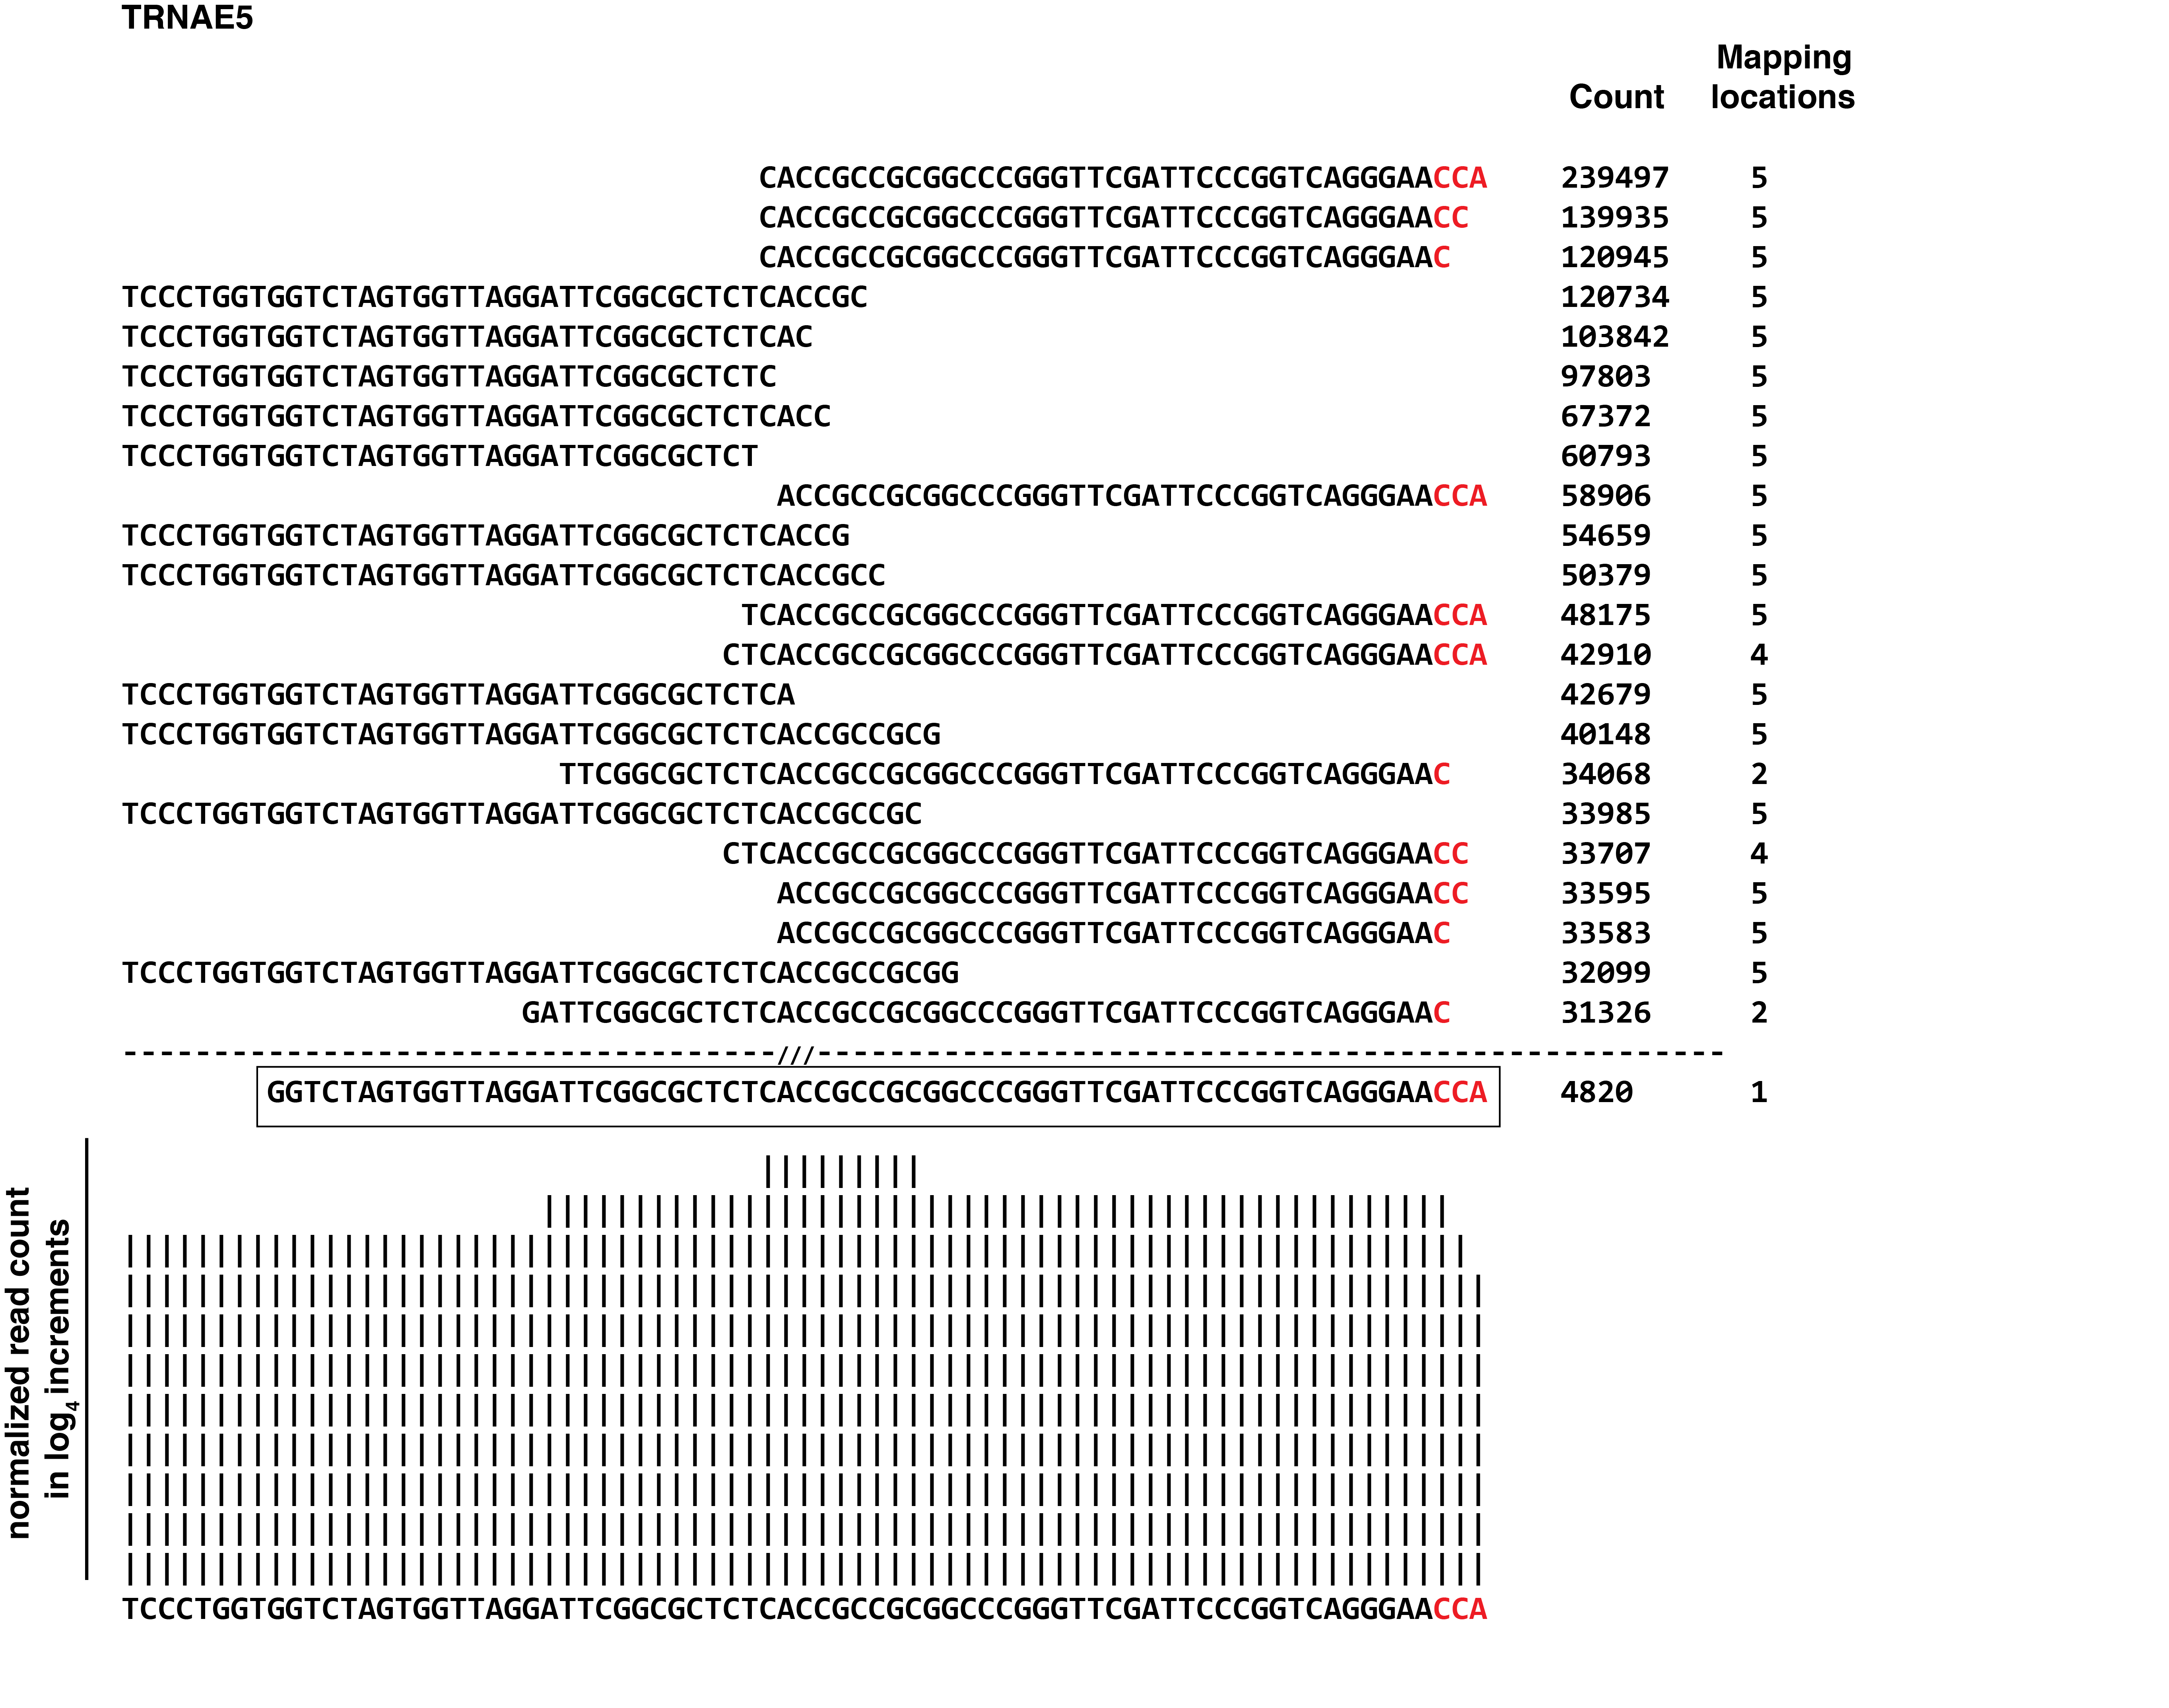
\includegraphics[width=\textwidth]{mature.png}%
\caption[Mature tRNA alignment]{\textbf{Mature tRNA alignment.} An indicative alignment to mature TRNAE5 is shown including, sequences of reads, abundance, mapping locations, and log\sub{4} bin-normalized abundance.}
\centering
\label{mature}%
\end{figure}

\textbf{Figure \ref{mature}} shows a representative alignment of reads to a mature glutamate-tRNA reference (TRNAE5). The name of the transcript is shown at the top, and the reference transcript sequence at the bottom of the file. Pile-ups of of reads that were mapped to the reference are sorted in descending order of abundance, shown in the 'count' column. Due to the intentional fragmentation of input RNA, we observe that the majority of reads were shorter than the full length tRNA, longer reads (like the one boxed at the lower part of the alignment) are used to bridge together separate segments. The total mapping locations for multimapping reads are also indicated.  Vertical lines represent the relative frequency of binned, normalized read count in log\sub{4} increments. The 3’ CCA aminoacyl acceptor terminus is shown in red indicating the hydro-tRNAseq is successful in freeing the terminus from charged amino acids. 

\subsection{Pre-tRNA alignment}
As part of the hierarchical mapping protocol, reads that are not accounted for during the generation of mature tRNA alignments are mapped to our curated pre-tRNA reference sequences, which span 40 nt up- and downstream from all mature tRNA boundaries. \textbf{Figure \ref{pre}} shows a representative alignment of reads to a glutamate pre-tRNA reference (TRNAE26), similar to \textbf{Fig. \ref{mature}}. The mature sequence is shown in blue, while the leader and trailer sequences in green. 

\begin{figure}[!ht]%
\centering
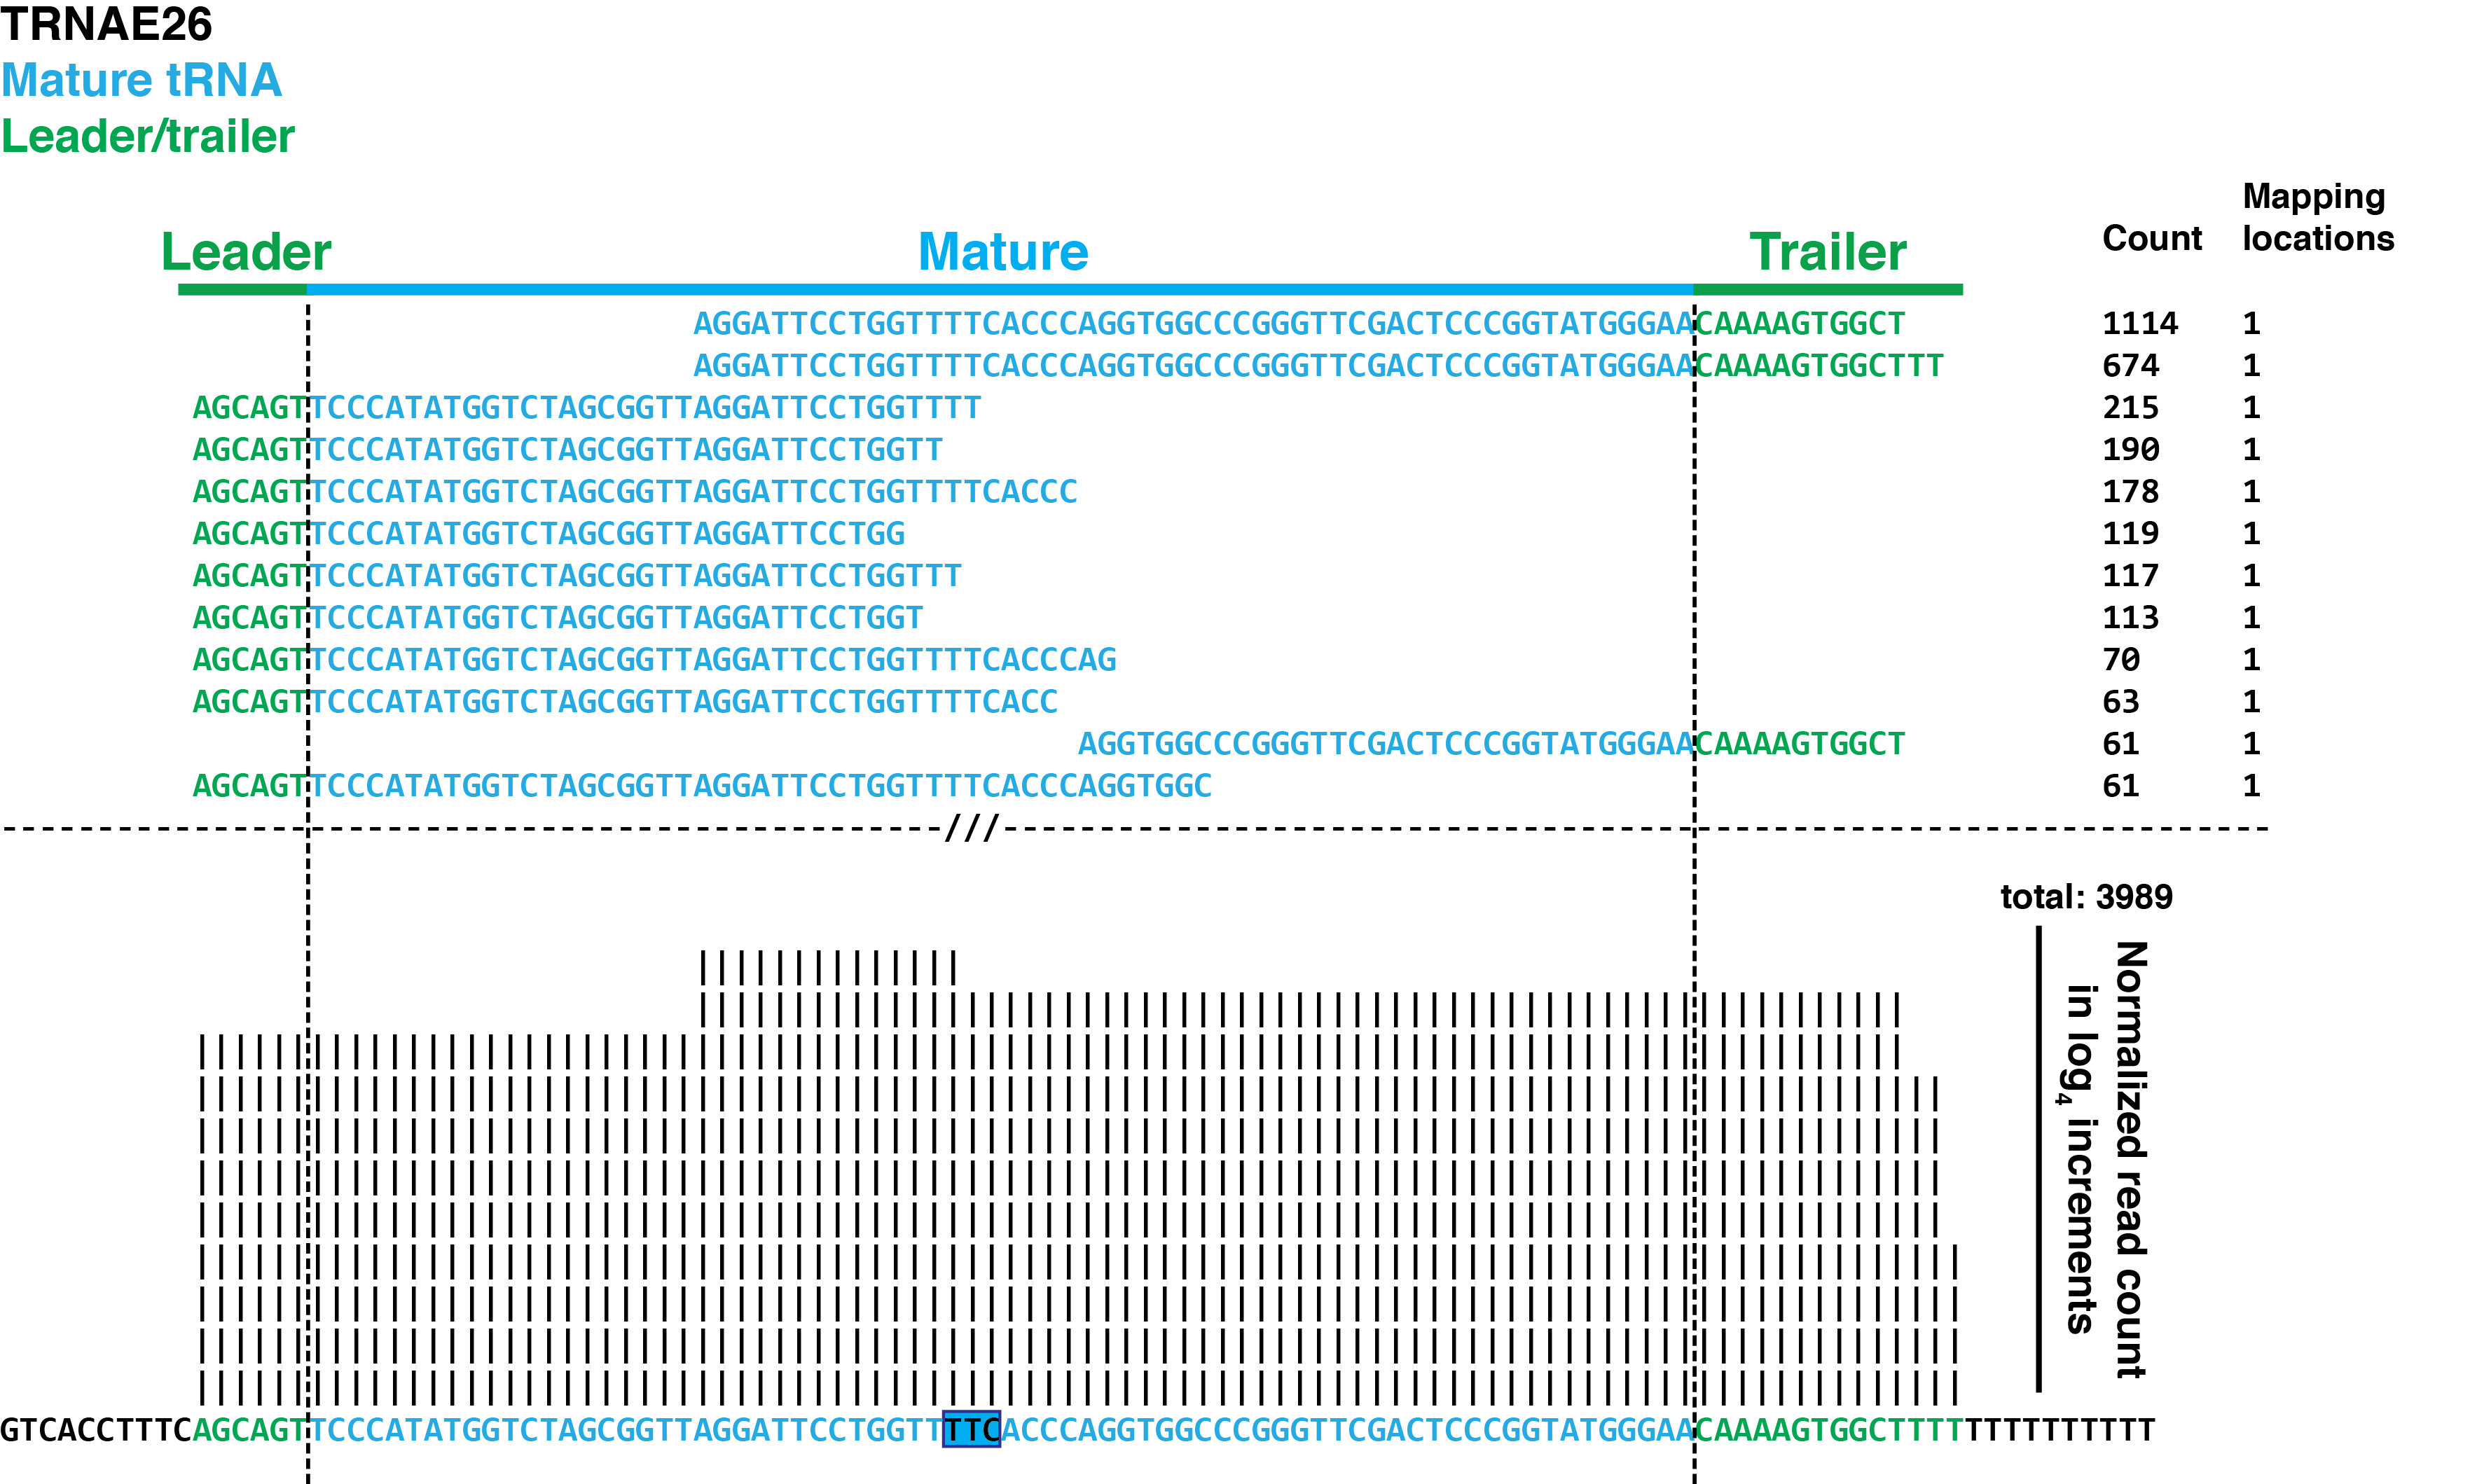
\includegraphics[width=5in]{pre.png}%
\caption[Pre-tRNA alignment]{\textbf{Pre-tRNA alignment.} An indicative alignment to pre-tRNA TRNAE5 is shown. Mature sequence is in blue and precursor-specific sequence segments in green. The anticodon is boxed in blue for orientation purposes.}
\centering
\label{pre}%
\end{figure}

The simplicity of the output files of our pipeline renders them easily exploitable for downstream bioinformatics analysis, necessitating only intermediate programming skills. At the same time the alignment displays can be used directly in figure making. As a matter of fact, simple, and easily customizable perl and python scripts were used for all the analysis presented in section \ref{applications}, showcasing the ease of primary sequence data access and analysis conferred by our approach.

\section{Need for pre-tRNA enrichment}
The majority of our reads obtained from 60-100 nt size-fractionated total RNA were assigned to mature tRNAs. The improvement we observed in recovering tRNA reads was considerable, as 2/3 of our reads mapped to either mature (nuclear or mitochondrial) or pre-tRNAs. Nevertheless, only 1\% of total reads comprised sequences overlapping with pre-tRNA leader or trailer sequences (\textbf{Fig. \ref{paper2a}, \ref{tableS1}}). This raised the possibility that we might have missed reads corresponding to lowly expressed or very rapidly processed pre-tRNAs.
\begin{figure}[!ht]%
\centering
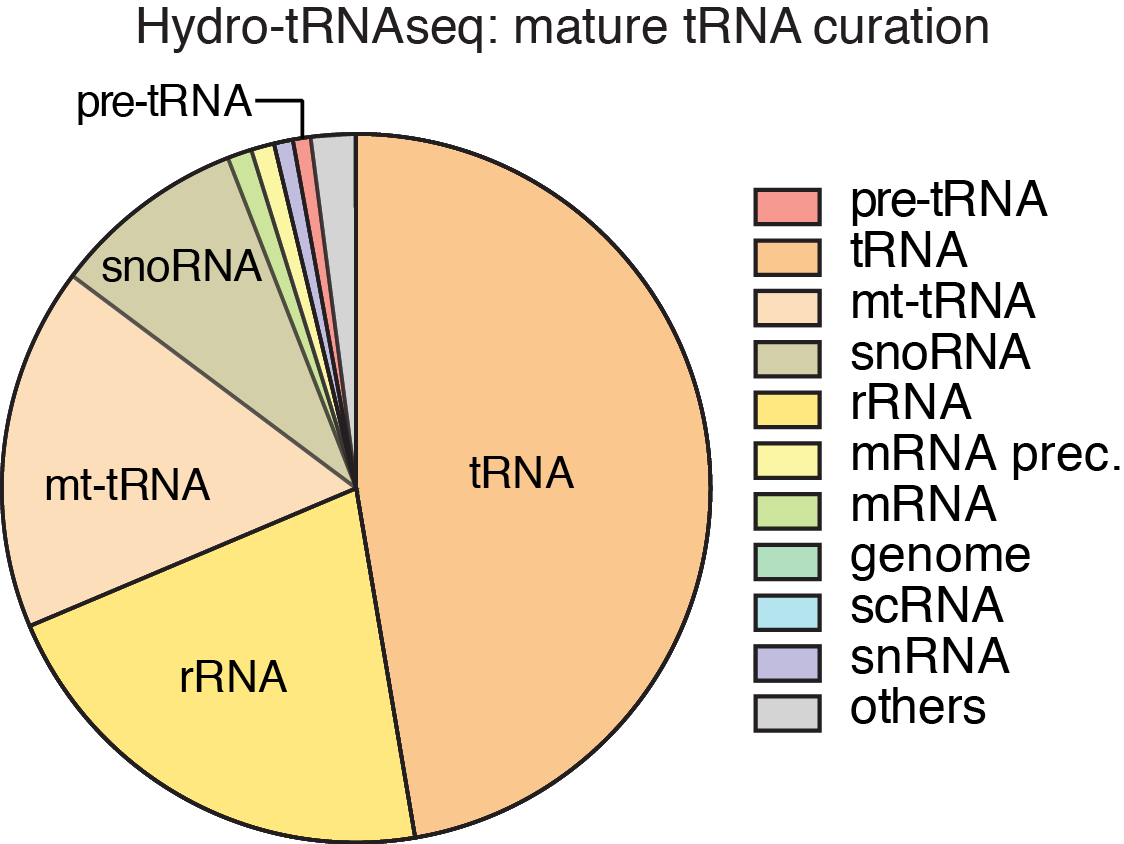
\includegraphics[width=4in]{paper2a.png}%
\caption[Composition of hydro-tRNAseq libraries]{\textbf{Composition of hydro-tRNAseq libraries.} Total RNA composition of the 60-100 nt size fraction from hydro-tRNAseq according to RNA classes.}
\centering
\label{paper2a}%
\end{figure}
We did this by performing \gls{parclip}, a technique developed in our lab to identify RNA targets of \glspl{rbp} with high specificity. 

\section{PAR-CLIP methodology for the study or RNA-RBP interactions}
A series of techniques have been developed for the study of RNA-RBP interactions on a genomic scale \cite{Konig:2011jv}. Our lab developed PAR-CLIP, coupled with deep sequencing, which is a cell-based approach that allows the determination of RBP binding sites on RNA targets at nucleotide-level resolution (\textbf{Fig. \ref{parclip}}\cite{Hafner:2010kr}). To enable efficient RNA-RBP crosslinking using long wavelength UV light, \gls{4su} is added to culture medium, taken up by cells and incorporated into nascent transcripts. The crosslinked ribonucleoprotein complex is submitted to partial RNase digestion, immunopurification and size-fractionated. Crosslinked RNA is recovered, converted into small RNA cDNA libraries, and sequenced. Importantly, crosslinking introduces a structural change in the thiouridine base, which allows pinpointing the position of crosslinking by scoring for characteristic T-to-C transitions in the sequenced cDNA. In addition, the abundant background derived from non-crosslinked fragments of co-purifying cellular RNAs do not contain these T-to-C transitions and can be filtered out. Thus, PAR-CLIP has a very low rate of false positive target identification, since the nucleotide transition signature reliably marks true crosslinking sites. PAR-CLIP has so far been applied successfully to the study of mRNA- and miRNA-binding proteins, but not \glspl{trbp}.

\begin{figure}[!ht]%
\centering
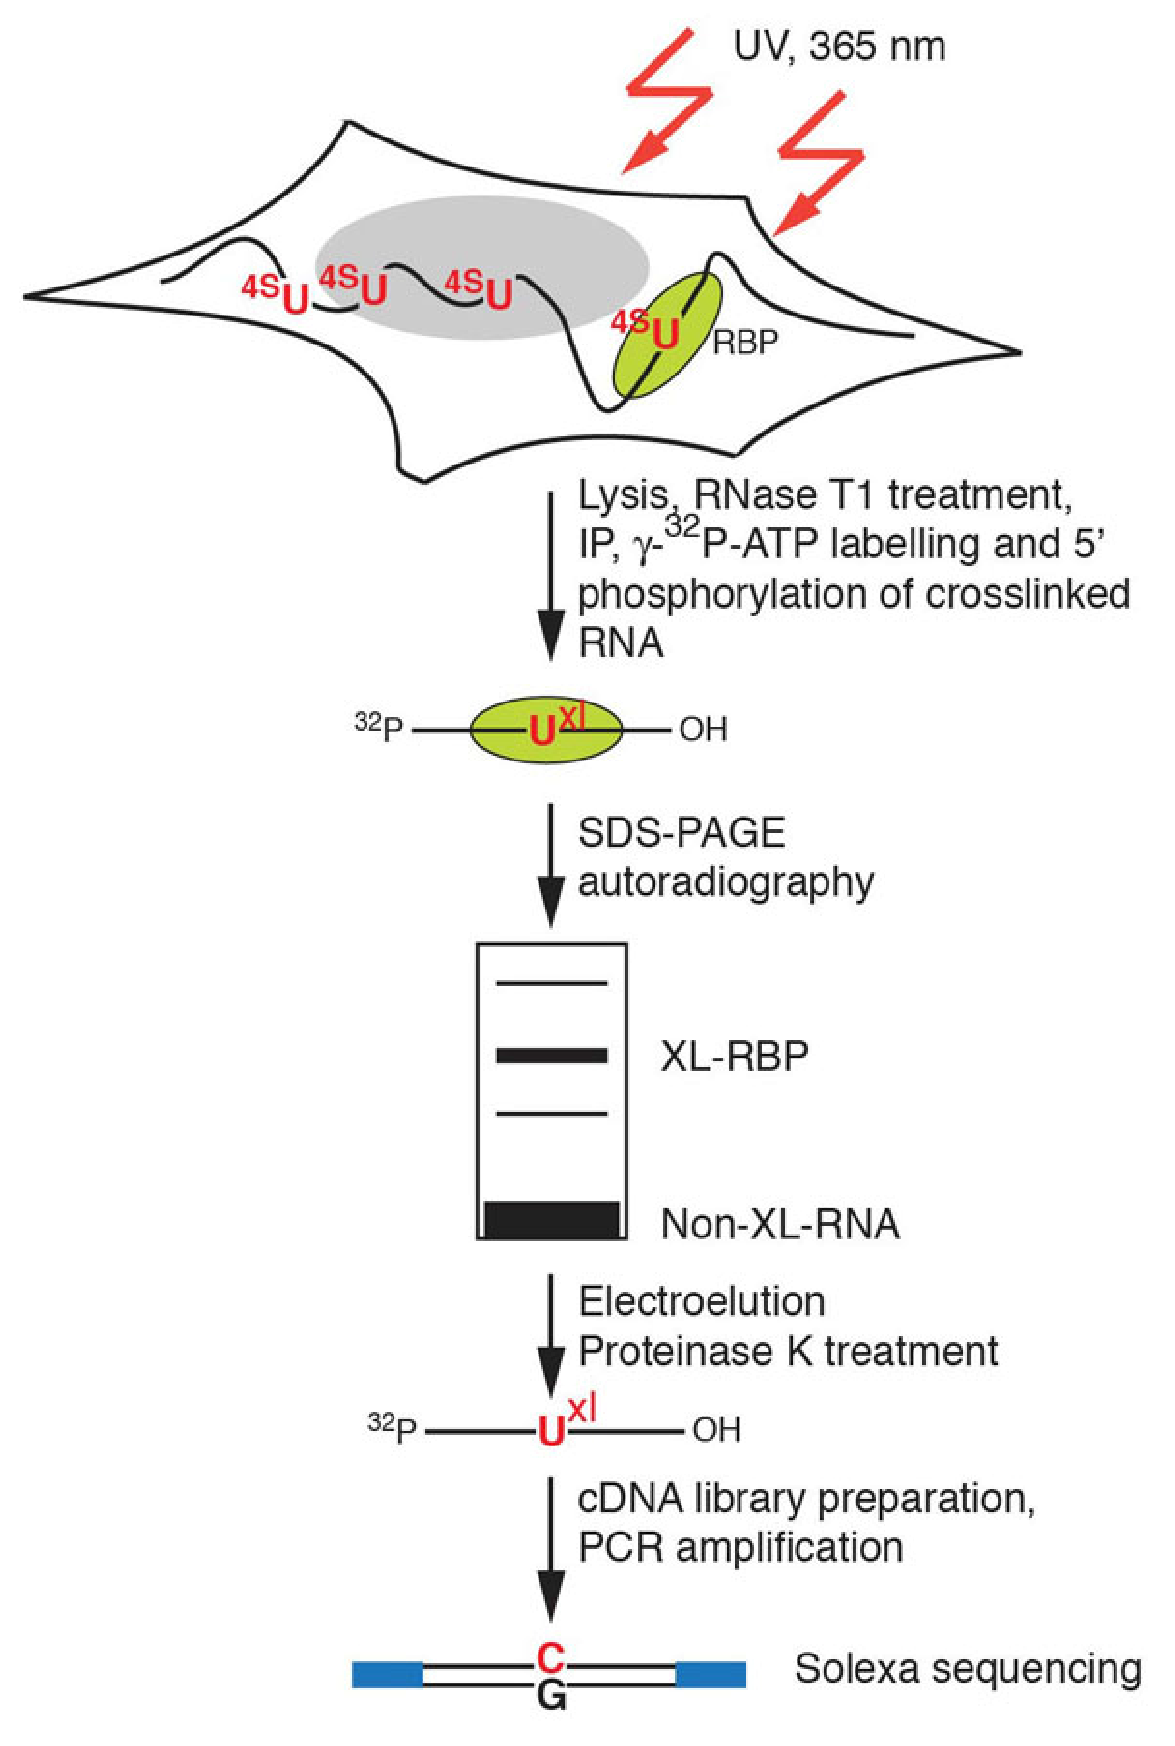
\includegraphics[width=3.5in]{parclip.png}%
\caption[PAR-CLIP]
{\textbf{PAR-CLIP.}
Outline}
\centering
\label{parclip}%
\end{figure}

\section{SSB PAR-CLIP}
Therefore, in collaboration with Aitor Garzia, we decided to complement our sequencing efforts with PAR-CLIP-sequencing of the protein \gls{SSB}, which is also known as \gls{La} (\textbf{Fig. \ref{paper2b}}). SSB has been shown biochemically to bind to the short 3’ oligoU tails \cite{Stefano:1984wp} that acts as termination signal for POLR3 \cite{Maraia:2010kx}. Therefore, we reasoned that SSB should bind all tRNA precursors, and that if we could isolate its targets, we would be able to reliably identify transcribed tRNA loci. 

\begin{figure}[!ht]%
\centering
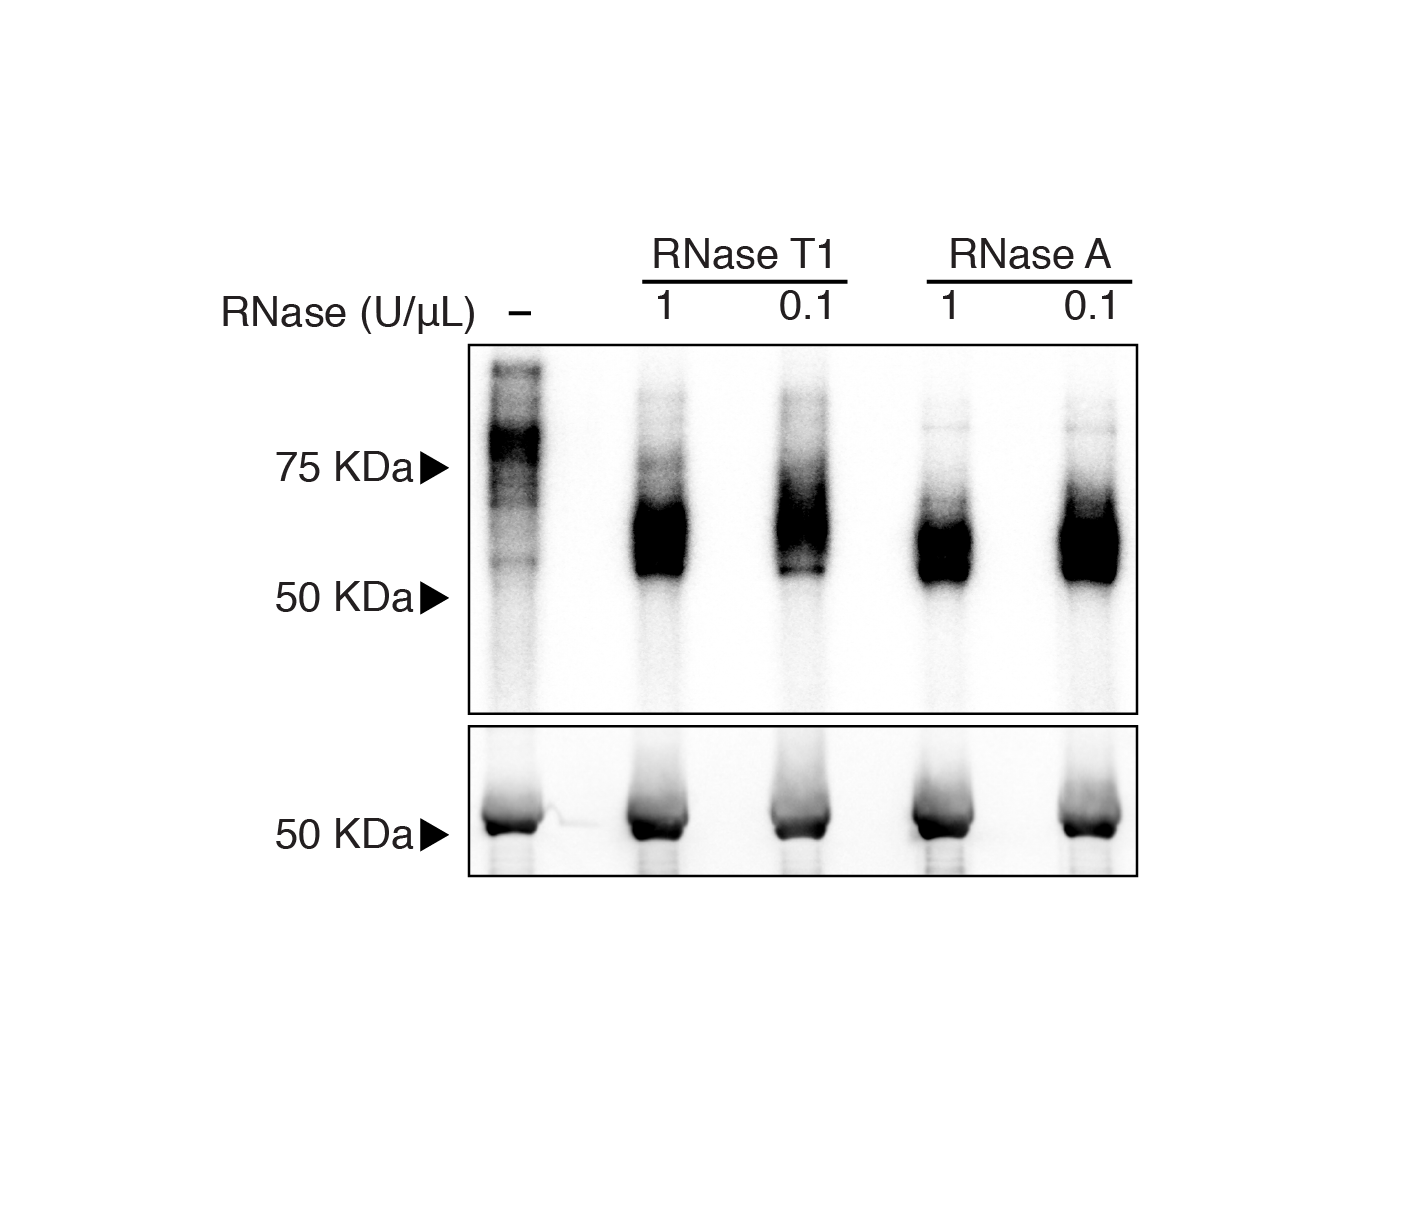
\includegraphics[width=4in]{paper2b.png}%
\caption[SSB crosslinking to RNA]
{\textbf{SSB crosslinking to RNA.}
Phosphorimage of SSB-crosslinked to radiolabeled RNA. PAR-CLIP was performed using RNase A or RNase T1, at two different concentrations to 
account for possible biases of RNase treatment conditions. Libraries from PAR-CLIP using 1 U/$\mu$L of RNase A and RNase T1 were prepared and submitted for sequencing. Western blot against HA, shown in the bottom, confirmed the immunoprecipitation of SSB.}
\centering
\label{paper2b}%
\end{figure}

\begin{table}[!ht]
  \begin{adjustbox}{max width = \textwidth}
%  \def\arraystretch{1.2}

  \begin{tabular}{|l|r|r|r|r|r|}
\hline
              Type &  \multicolumn{1}{l|}{D0 counts} &  \multicolumn{1}{l|}{D1 counts} &  \multicolumn{1}{l|}{D2 counts} &  \multicolumn{1}{l|}{Total} & \multicolumn{1}{l|}{Percent of total} \\
\hline  
       pre-tRNA &  8,249,237 &  45,310,051 &  18,719,097 &  72,278,385 &              46\% \\
            tRNA &  8,687,821 &  16,903,928 &   7,278,511 &  32,870,260 &              21\% \\
            rRNA &  3,120,687 &  15,480,966 &   2,745,431 &  21,347,084 &              14\% \\
       mRNA gene &  1,446,452 &   4,200,866 &  10,423,676 &  16,070,994 &              10\% \\
            mRNA &    396,184 &   2,788,499 &   7,499,514 &  10,684,197 &               7\% \\
           scRNA &    243,364 &   1,543,873 &     305,333 &   2,092,570 &               1\% \\
    lincRNA gene &     81,146 &     224,548 &     335,874 &     641,568 &               0\% \\
         adapter &    282,626 &      90,077 &       8,183 &     380,886 &               0\% \\
           snRNA &     37,462 &     131,211 &      31,302 &     199,975 &               0\% \\
          snoRNA &     11,203 &      54,179 &      16,072 &      81,454 &               0\% \\
           miRNA &      3,228 &      17,382 &      20,827 &      41,437 &               0\% \\
      scRNA prec &      5,979 &      23,546 &       7,876 &      37,401 &               0\% \\
           piRNA &      8,573 &       1,671 &       9,102 &      19,346 &               0\% \\
         plasmid &      5,344 &       4,722 &       6,301 &      16,367 &               0\% \\
         mt rRNA &     11,006 &       2,866 &         979 &      14,851 &               0\% \\
         mt tRNA &      3,356 &       5,942 &       2,617 &      11,915 &               0\% \\
     snoRNA prec &        703 &       5,030 &       2,362 &       8,095 &               0\% \\
       rRNA prec &      2,076 &       3,549 &       1,548 &       7,173 &               0\% \\
         mt mRNA &      1,017 &       1,783 &       3,207 &       6,007 &               0\% \\
          scaRNA &        198 &       2,654 &       1,708 &       4,560 &               0\% \\
          marker &      1,739 &         208 &          27 &       1,974 &               0\% \\
         lincRNA &        698 &         515 &         714 &       1,927 &               0\% \\
       long cali &          3 &         151 &         662 &         816 &               0\% \\
  doubtful miRNA &        176 &         140 &         203 &         519 &               0\% \\
      snRNA prec &         13 &          66 &          37 &         116 &               0\% \\
     scaRNA prec &          6 &          37 &           7 &          50 &               0\% \\
         mirtron &          2 &          17 &           6 &          25 &               0\% \\
         circRNA &          0 &           0 &          14 &          14 &               0\% \\
        std cali &          0 &           1 &          10 &          11 &               0\% \\
        Ome cali &          0 &           2 &           5 &           7 &               0\% \\
        alt cali &          0 &           0 &           3 &           3 &               0\% \\
 doubtful snoRNA &          1 &           0 &           1 &           2 &               0\% \\
\hline
  \end{tabular}
  \end{adjustbox}
\caption[SSB PAR-CLIP reads per RNA type]{\textbf{SSB PAR-CLIP reads per RNA type.} Reads assigned to each RNA type following hierarchical annotation are shown. Reads with no (d0), one (d1) or two (d2) mismatches compared to reference are shown. Data from replicate using RNase T1 are shown. SSB PAR-CLIP enriches for pre-tRNAs (46\%).}\label{tableS3}
\end{table}

SSB exhibited a striking binding preference for pre-tRNAs and showed a drastic enrichment in precursor tRNAs compared to hydro-tRNAseq (\textbf{Fig. \ref{paper2cd}}), which confirmed our hypothesis, as well as previous observations \cite{Bayfield:2009cx}. We performed PAR-CLIP using two different nucleases to control for sequence biases at the nuclease digestion step. RNase T1 resulted in longer precursor tRNA trailer sequences than RNase A, due the latter’s preference for cleaving 3’ to pyrimidines, which are highly abundant in the 3’ trailer sequences. Overall, 46\% of all PAR-CLIP reads mapped to pre-tRNAs (\textbf{Fig. \ref{paper2cd}A}), the overwhelming majority of which showed the characteristic T-to-C transition, indicative of crosslinking (\textbf{Fig. \ref{paper2cd}B, Table \ref{tableS3}}).


\begin{figure}[!ht]%
\centering
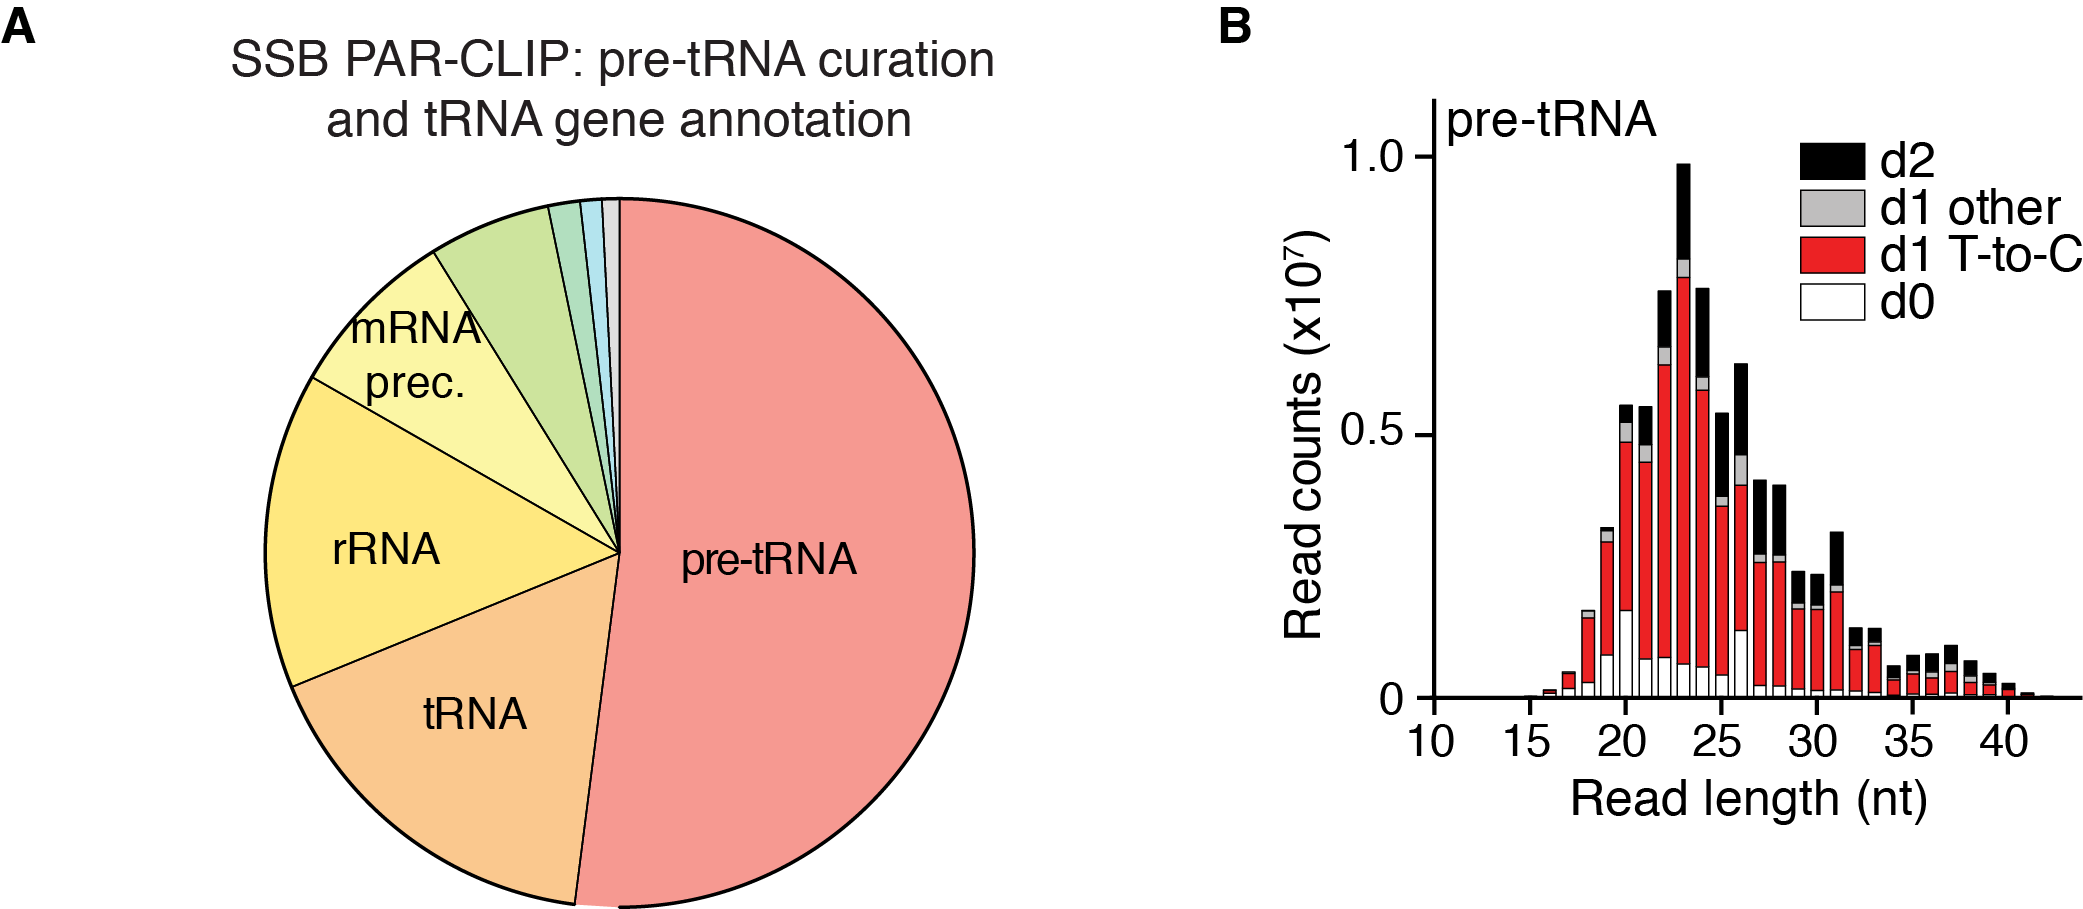
\includegraphics[width=\textwidth]{paper2cd.png}%
\caption[SSB binds pre-tRNAs.]
{
\textbf{SSB binds pre-tRNAs.}
(A) Assignment of reads from SSB PAR-CLIP (RNase T1, 1 U/µL) to RNA classes. (B) SSB PAR-CLIP reads mapping to tRNA precursors with 0, 1 or 2 mismatches (d0, d1, d2); reads with T-to-C mismatches are separated (red) from the rest of the reads with one mismatch (gray). Read length and number of reads are represented on the x- and y-axis, respectively. 
}
\centering
\label{paper2cd}%
\end{figure}

\begin{figure}[!h]%
\centering
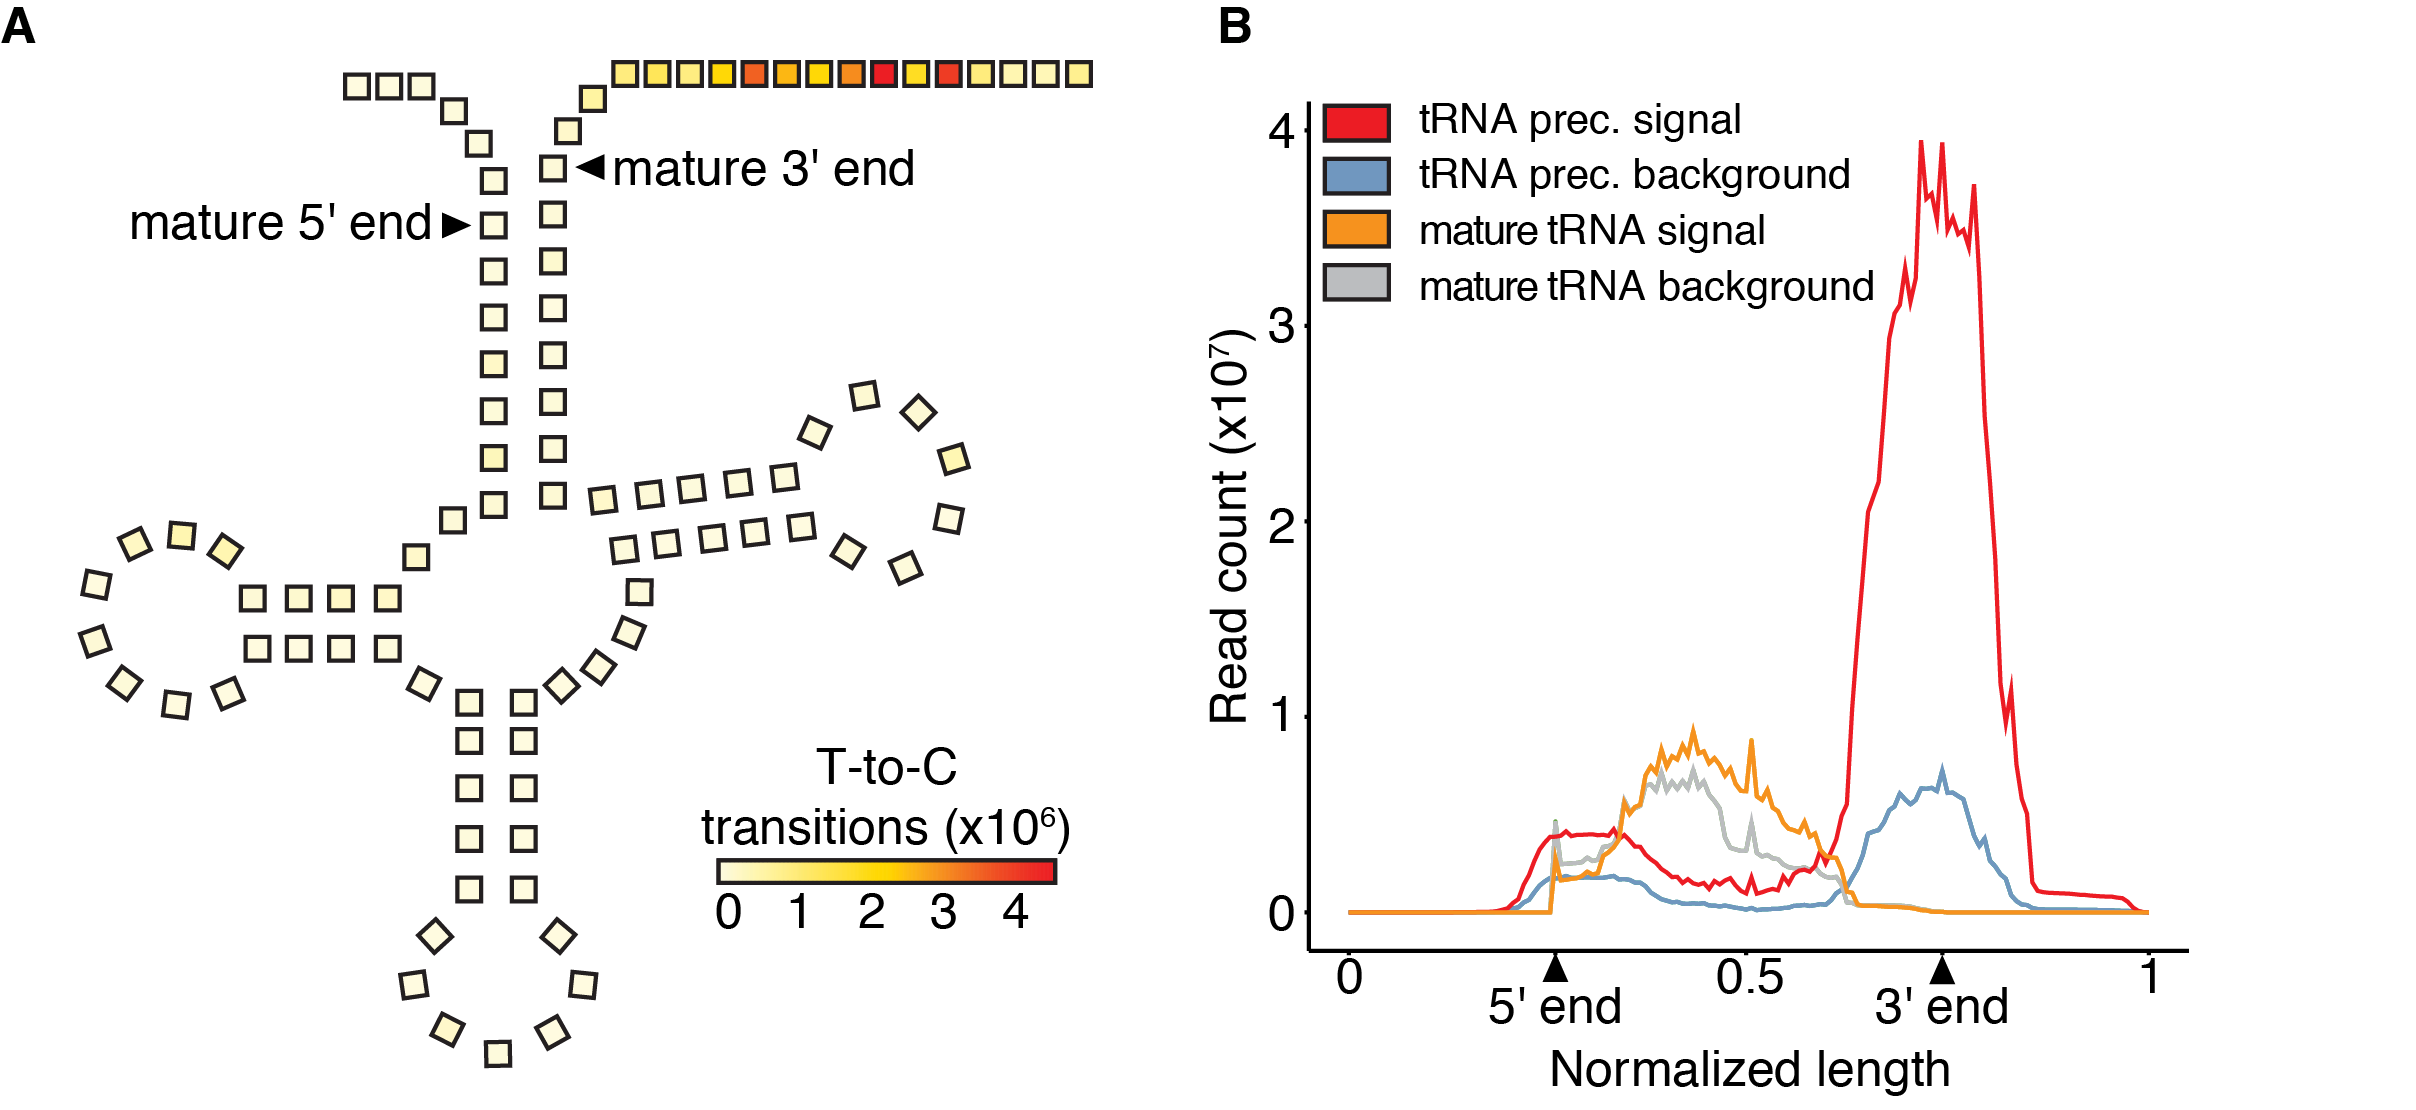
\includegraphics[width=\textwidth]{paper2ef.png}%
\caption[SSB binds the 3' oligoU stretch of pre-tRNAs.]
{
\textbf{SSB binds the 3' oligoU stretch of pre-tRNAs.}
(A) Positional preference of SSB crosslinking by metagene analysis of all crosslinking events to precursor tRNAs. The incidence of T-to-C transitions is indicated by color intensity. (B) Positional preference of SSB crosslinking by metagene analysis of reads mapped hierarchically; first to mature and then to precursor tRNAs. For each class, PAR-CLIP signal (reads containing T-to-C) and background (reads with no mismatches) are shown. The normalized boundaries of pre-tRNAs (labeled as 0,1) and mature tRNAs (labeled as 5’ end, 3’ end), and read count are shown on the x- and y-axis, respectively.
}
\centering
\label{paper2ef}%
\end{figure}

\begin{figure}[!h]%
\centering
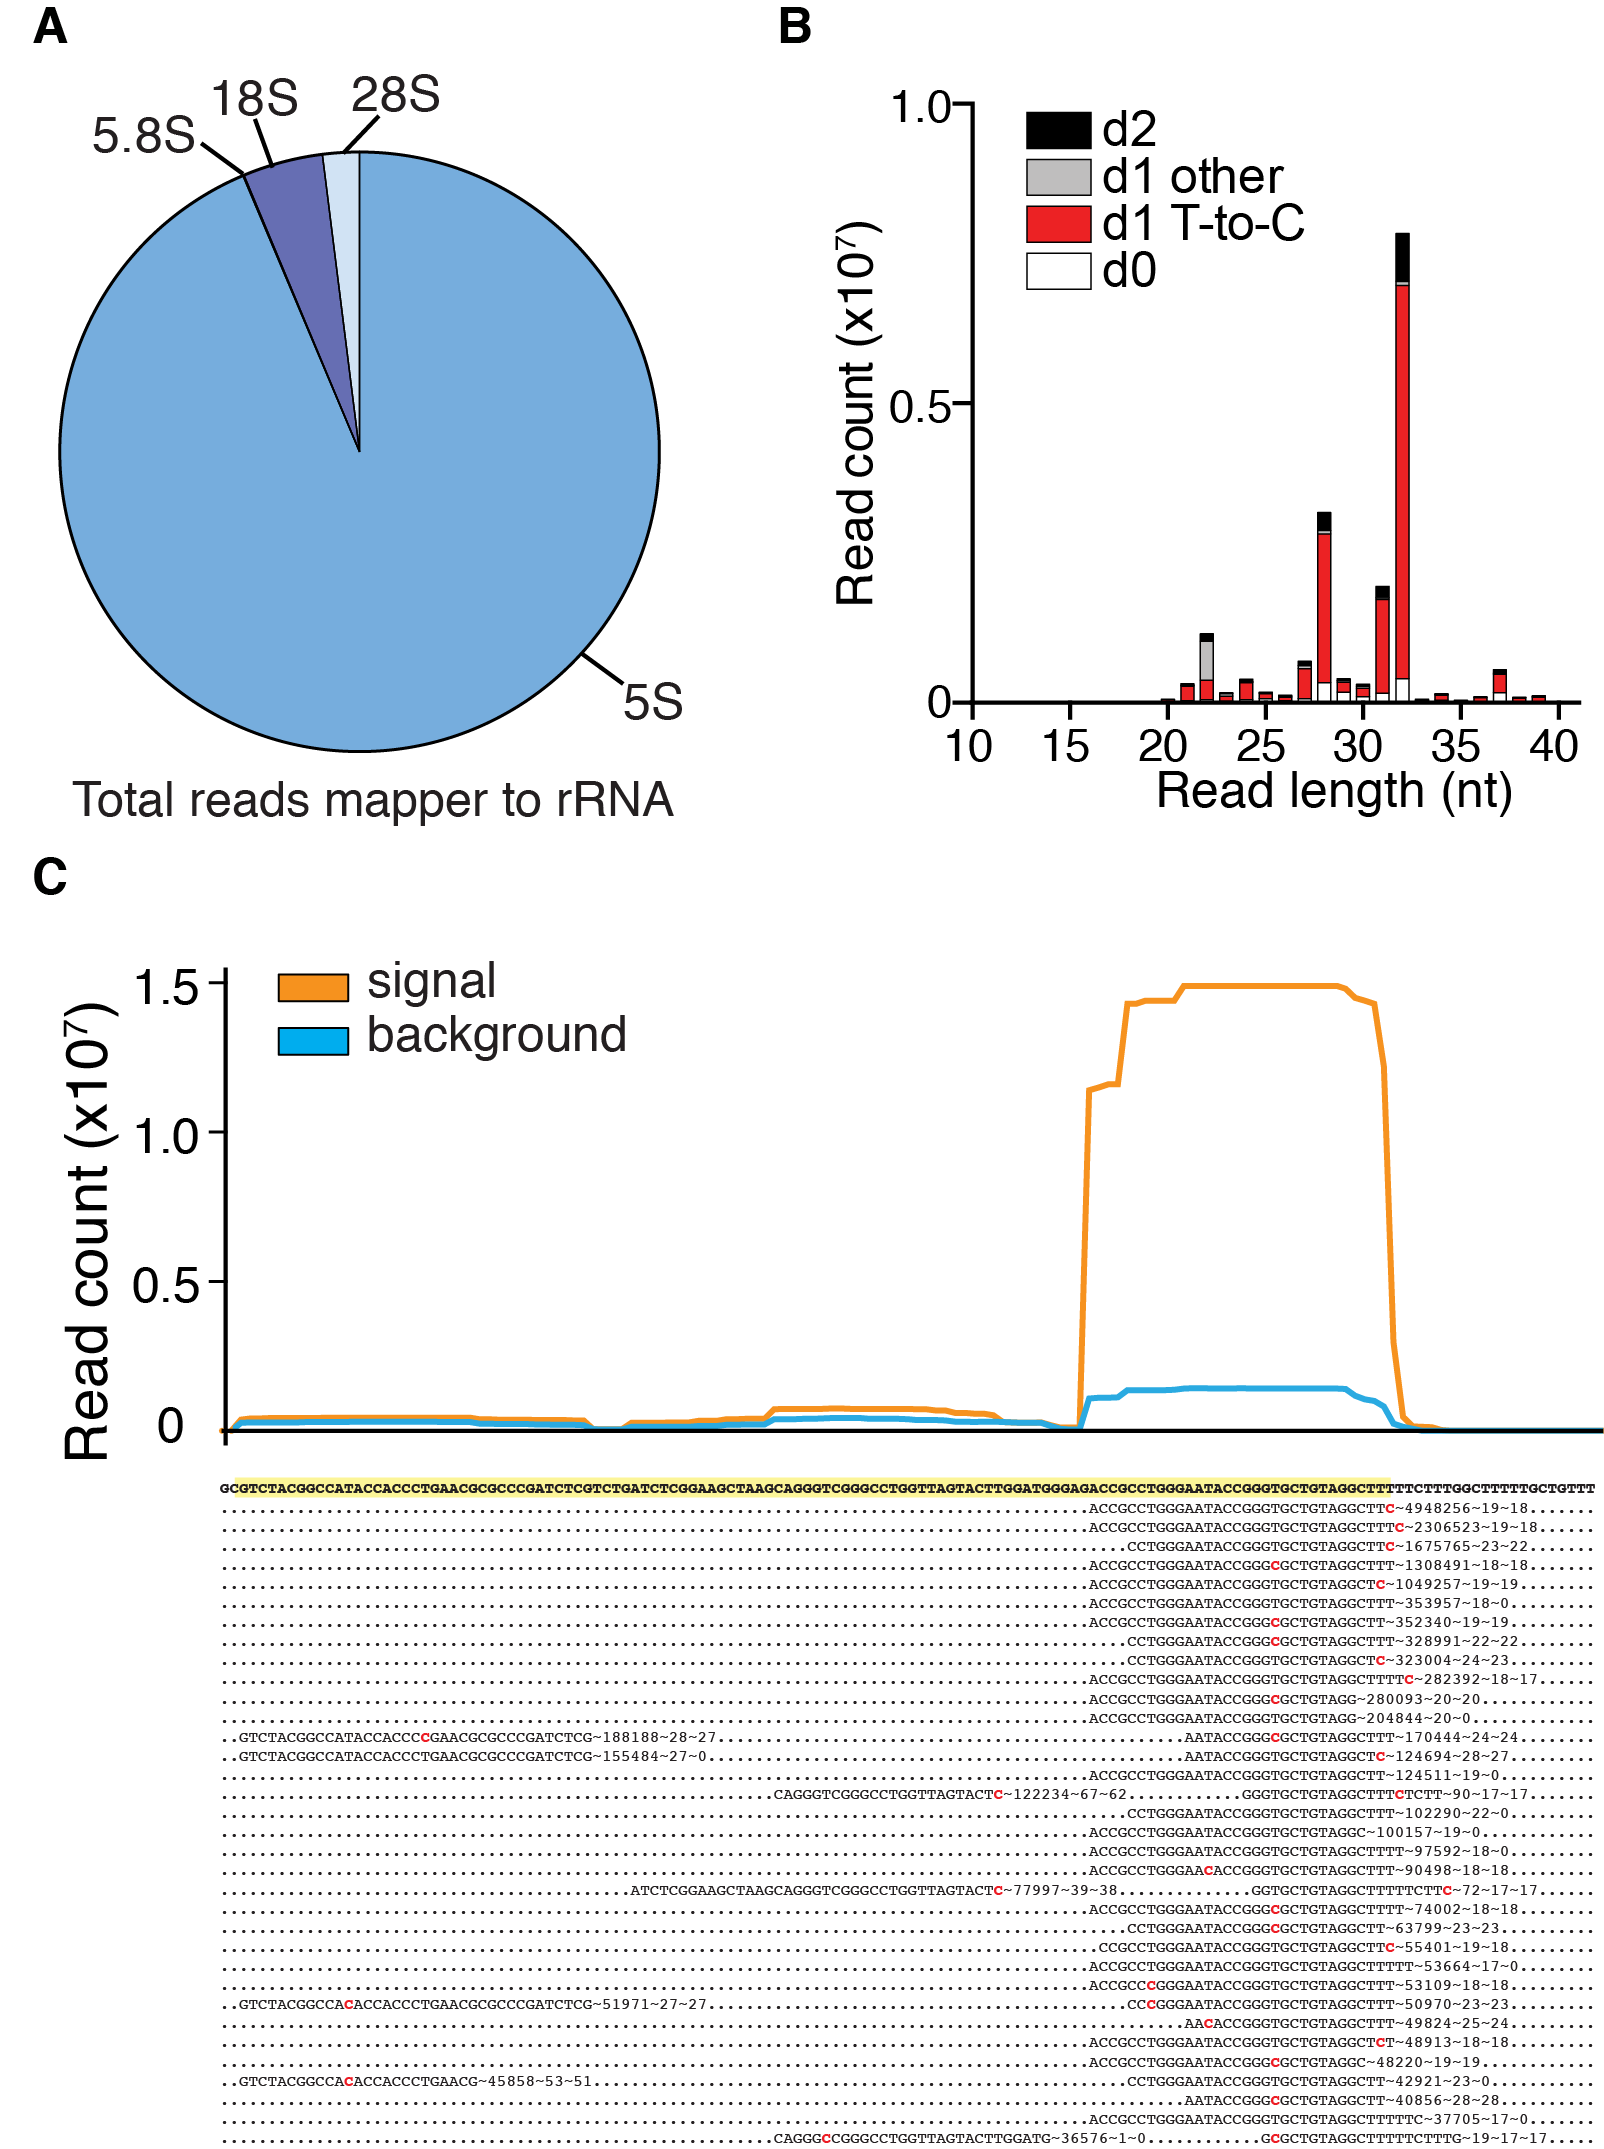
\includegraphics[scale = 0.8]{supp3.png}%
\caption[SSB binds 5S rRNA.]
{
\textbf{SSB binds 5S rRNA.}
(A) Assignment of reads from SSB PAR-CLIP to rRNAs. (B) Abundance of reads mapped to 5S rRNA with 0, 1 or 2 mismatches (d0, d1, d2) as a function of read length; reads with T-to-C mismatches are separated (red) from the rest of the reads with one mismatch (gray). Read length and number of reads are represented on the x- and y-axis, respectively. (C) Read alignments corresponding to 5S rRNA. Crosslinked positions are shown in red. The read count is shown next to each read sequence, followed by the total mapping positions, and the mapping positions that contain a T-to-C transition. Crosslinked and non-crosslinked read coverage is graphically represented.
}
\centering
\label{supp3}%
\end{figure}

The vast majority of crosslinking sites in pre-tRNAs were concentrated, as expected, in the oligoU tract of the 3’ trailer sequence (\textbf{Fig. \ref{paper2ef}}). We also found that SSB crosslinked to the 5’ segment of the mature tRNA body at conserved sites in the D-stemloop (\textbf{Fig. \ref{paper2ef}B}), which is a novel finding, hinted at by a report proposing that the affinity of SSB for a full-length pre-tRNA cannot be explained solely by its binding to the 3’ oligoU tract \cite{Bayfield:2009cx}. The other major target of SSB was 5S ribosomal RNA (rRNA), which is the only POLR3-transcribed rRNA, and, as such,	 also terminates with an oligoU stretch to which SSB crosslinked (\textbf{Fig. \ref{supp3}}). 


\section{tRNA gene annotation}
I combined hydro-tRNAseq and SSB PAR-CLIP to identify actively transcribed tRNA genes (genomic locations that give rise to a supported pre-tRNAs). I could confidently identify 288 tRNA genes as the intersection of 4 replicates of hydro-tRNAseq (\textbf{Fig. \ref{paper3}A}), and 349 tRNA genes as the intersection of two SSB PAR-CLIP experiments (\textbf{Fig. \ref{paper3}B}). Of note, SSB PAR-CLIP confirmed the expression of an additional 7 tRNA genes that were not supported in hydro-tRNAseq replicate (\textbf{Fig. \ref{paper3}C}), further showcasing the complementarity of the two approaches. There was a strong correlation of pre-tRNA abundances between SSB PAR-CLIP and hydro-tRNAseq (Pearson R = 0.72; \textbf{Fig. \ref{paper3}D}), providing confidence that SSB PAR-CLIP quantitatively detected pre-tRNAs, without introducing biases (e.g. artificially enriching for lowly expressed pre-tRNAs). The correlation of identified isoacceptor counts between SSB PAR-CLIP and hydro-tRNAseq was virtually perfect (Pearson R = 0.99; \textbf{Fig. \ref{paper4}A}), ruling out the introduction of a pronounced systematic bias from our hydrolysis-based protocol. Some anticodons seemed to be served by multiple isodecoders (e.g. 19 isodecoders for tRNA\textsuperscript{Ser}\textsubscript{GCA}), while others only from one (e.g. tRNA\textsuperscript{Ser}\textsubscript{ACT};(\textbf{Fig. \ref{paper4}B}).Selenocysteine was the only amino acid that, in our data, was decoded by only one tRNA gene.

\begin{figure}[!h]%
\centering
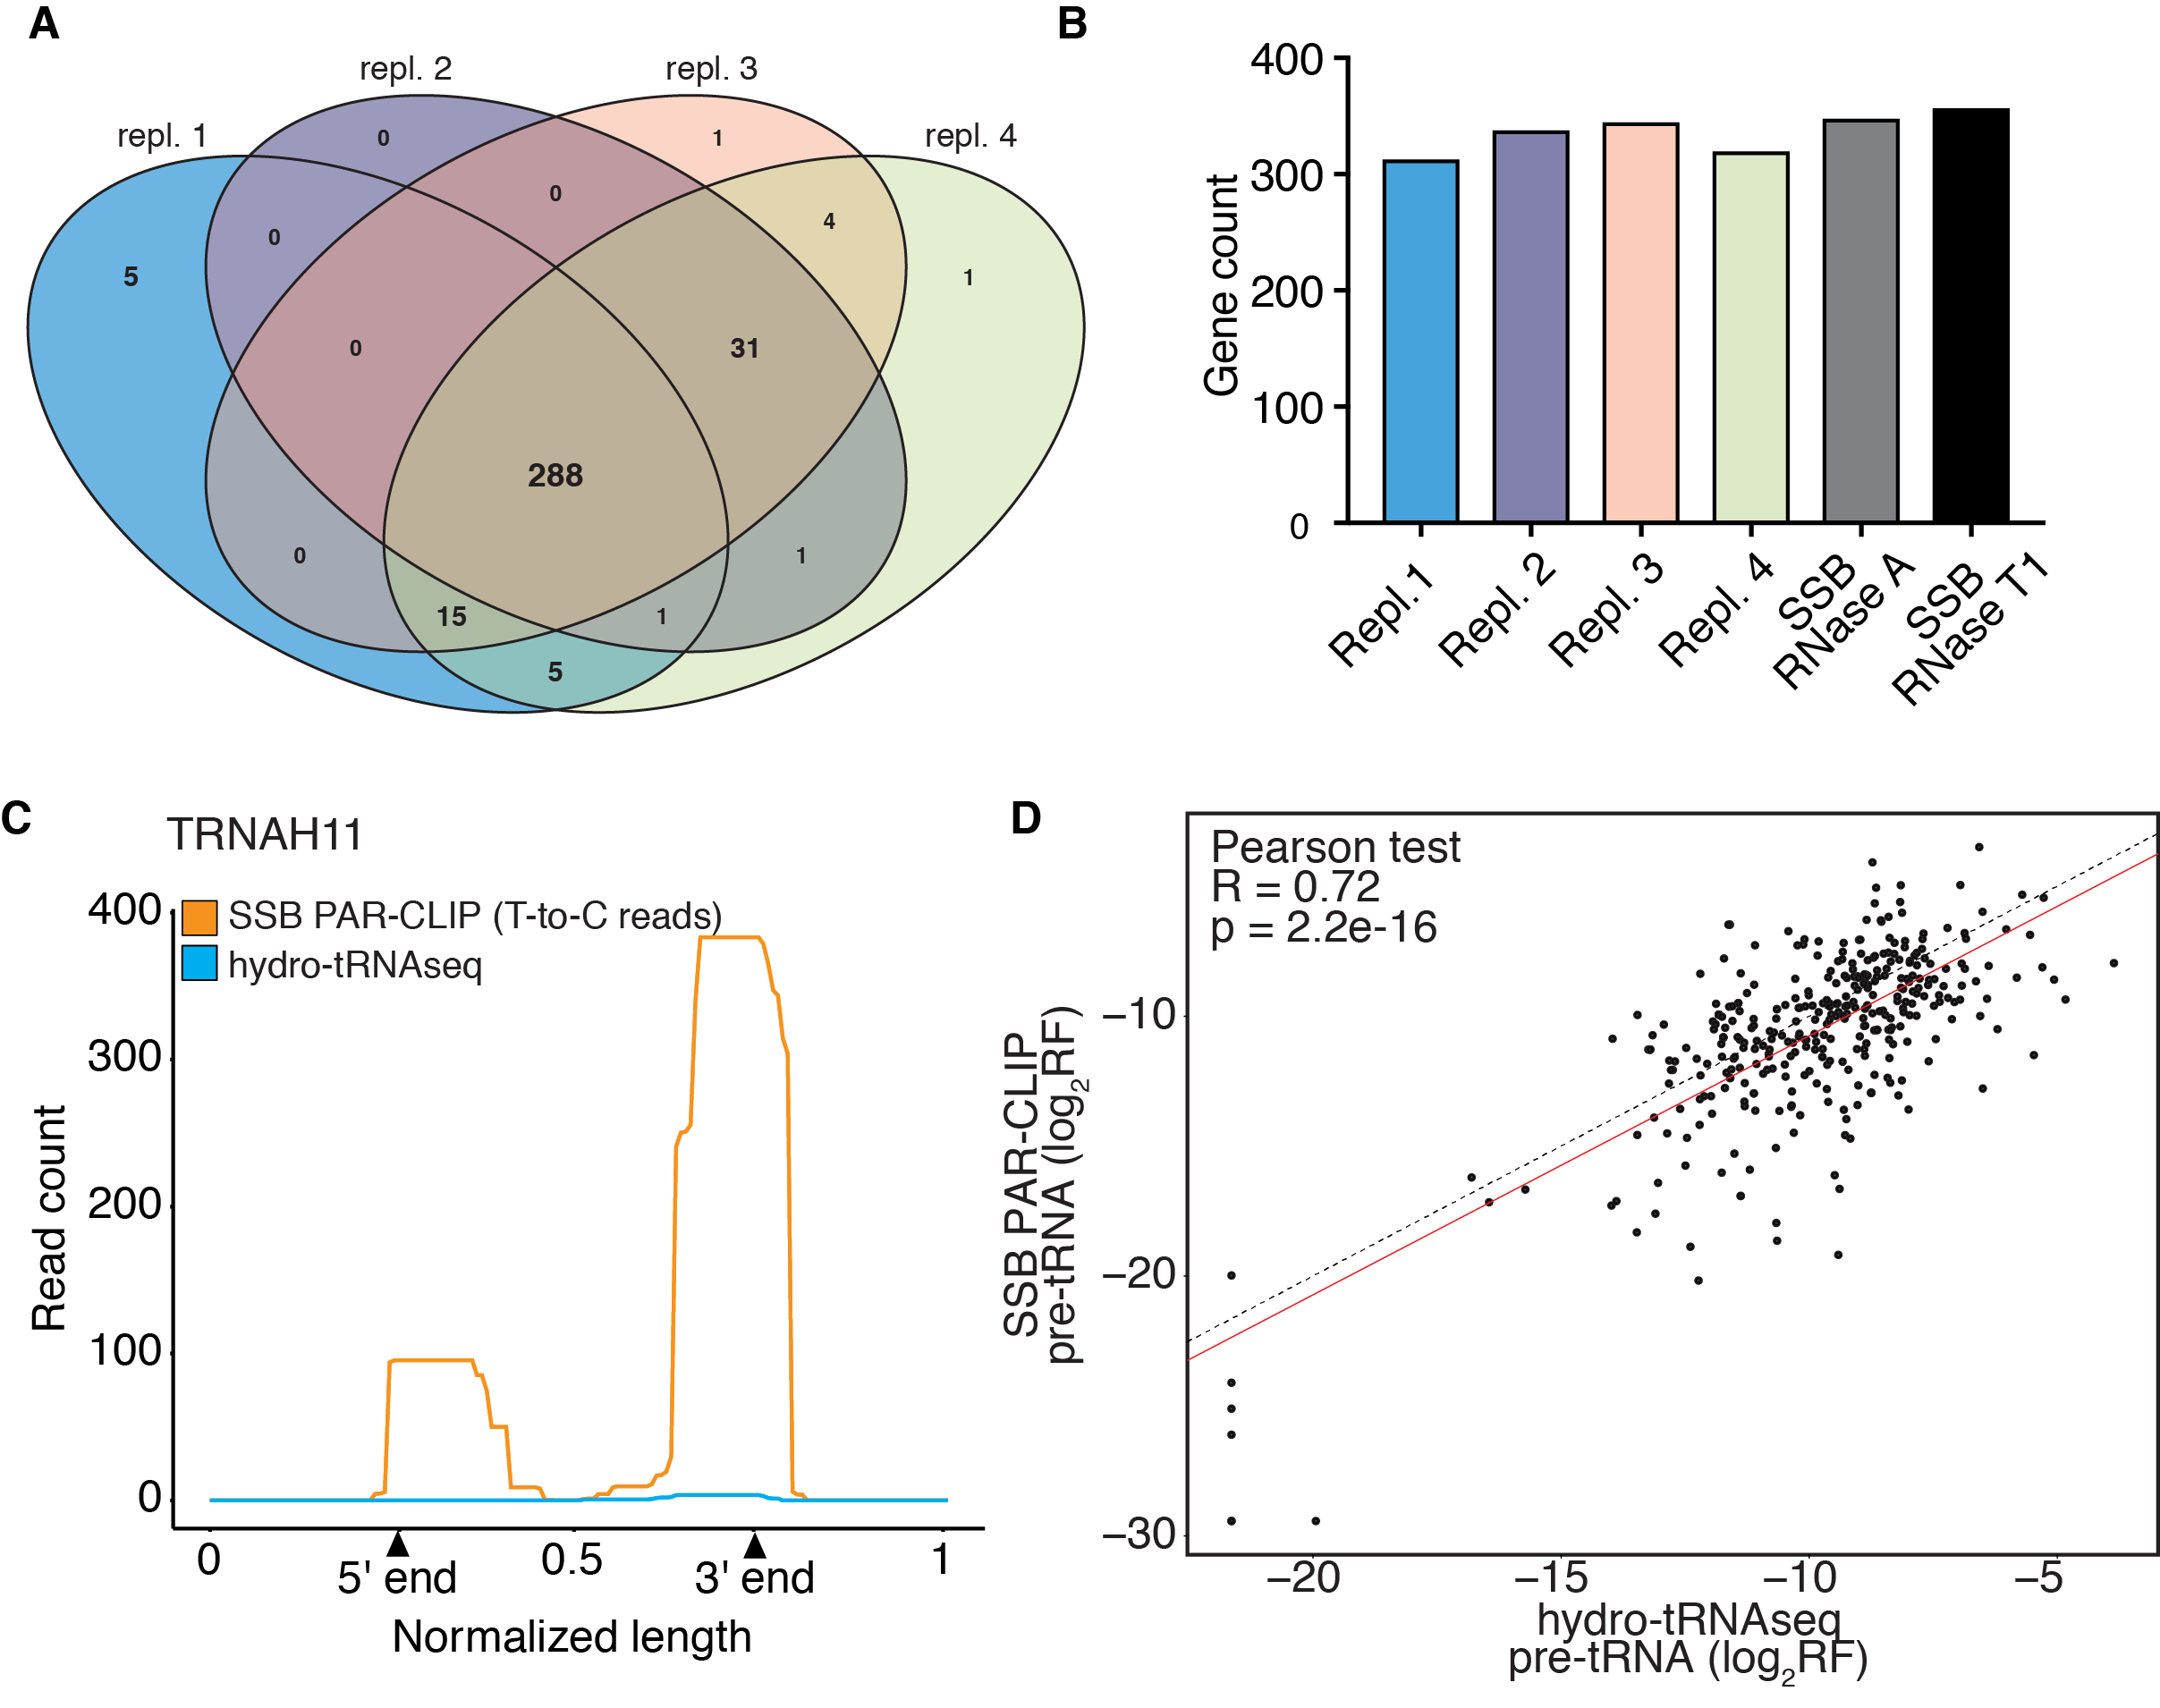
\includegraphics[width=\textwidth]{paper3.png}%
\caption[tRNA gene annotation.]
{\textbf{tRNA gene annotation.}
(A) Venn diagram of expressed tRNA genes detected by hydro-tRNAseq in HEK293 cells. Genes with read evidence in both the 5’ leader and 3’ trailer of the pre-tRNA were counted. (B) Bar chart showing the number of pre-tRNAs detected in each replicate of hydro-tRNAseq and SSB PAR-CLIP. (C) Example of one out of seven tRNA genes that were detected by SSB PAR-CLIP, but were not detected in any of four hydro-tRNAseq replicates. (D) Correlation of relative read frequencies (log2-transformed) of precursor tRNAs between hydro-tRNAseq (x-axis) and SSB PAR-CLIP (y-axis). Correlation was calculated using the Pearson test. Linear fit is shown in red. The y=x line (dotted) is shown for comparison.}
\centering
\label{paper3}%
\end{figure}

\begin{figure}[!h]%
\centering
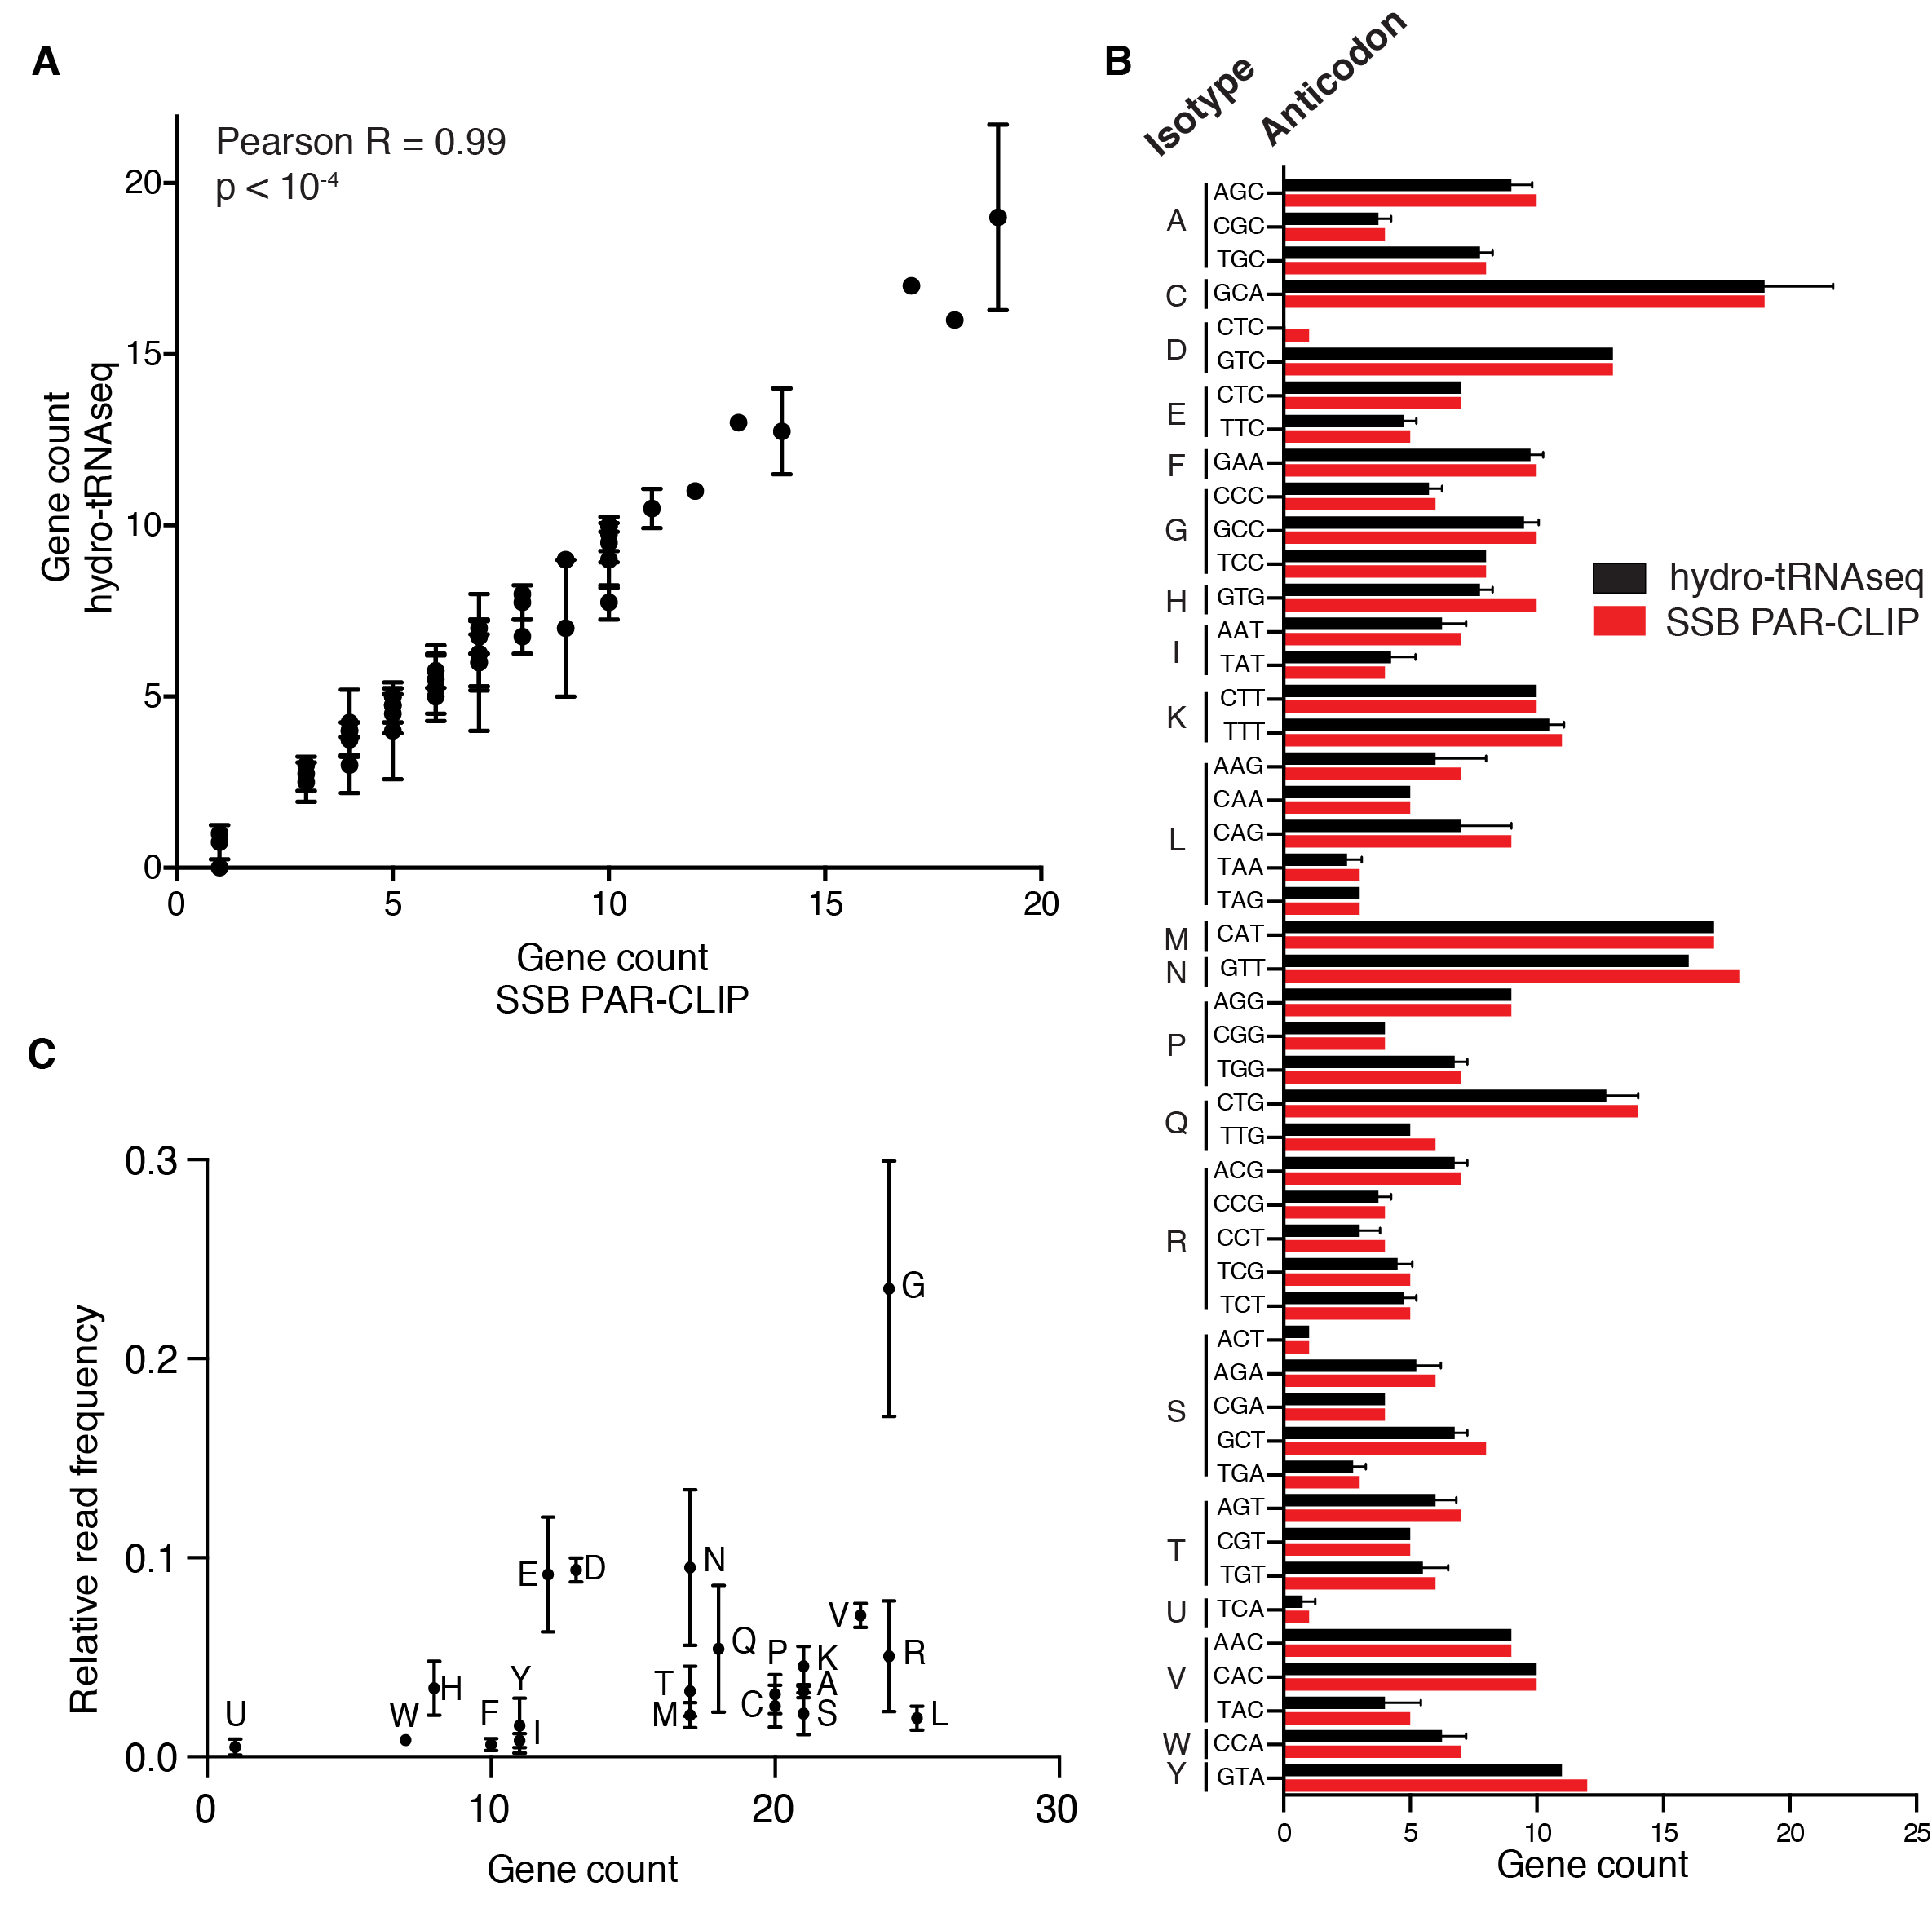
\includegraphics[width=\textwidth]{paper4.png}%
\caption[Number and relative abundance of tRNA genes per isotype and isoacceptor.]
{\textbf{Number and relative abundance of tRNA genes per isotype and isoacceptor.}
(A) Correlation of gene counts for each anticodon detected by hydro-tRNAseq (y-axis) and SSB PAR-CLIP (x-axis). Each dot represents an anticodon shown in (B). Correlation was calculated using the Pearson test.(B) Number of tRNA genes for each anticodon and isotype. Hydro-tRNAseq data are shown in black (mean of 4 replicates; error bars represent standard deviation), SSB PAR-CLIP (RNase T1 treated) in red. (C) Correlation of relative read frequency (y-axis) of mature tRNAs with number of genes (x-axis) per tRNA isotype. Hydro-tRNAseq data; four replicates; mean values shown; error bars represent standard deviation.}
\centering
\label{paper4}%
\end{figure}

\chapter{Applications and biological insights}\label{applications}

\section{tRNA gene abundance does not correlate with tRNA gene count on the isotype level}

Having established the rigor and validity of our experimental and computational method, we set out to address long-standing questions related to tRNA biology. First, we asked whether there is a linear relationship between number of tRNA genes (which will from now on be used interchangeably with pre-tRNAs) and the collective abundance of tRNAs for a given isotype. Due to the absence of reliable tRNAseq datasets, it was assumed that tRNA abundance increased monotonically with increasing tRNA gene count \cite{Iben:2014dt,Pechmann:2012ey,Tuller:2010ge}. 

This proposition hinged on the assumption that tRNAs undergo insignificant transcriptional or post-transcriptional regulation gene regulation, and thus all tRNA genes are transcribed and contribute equally to the mature tRNA abundance. It dismissed, thus, any possible mechanisms of affecting steady state tRNA levels, such as modulation of transcription, processing and degradation. 

Indeed, recent data, albeit scant and based on array-type experiments, suggested that the tRNA repertoire can be regulated in a dynamic fashion, and might not even be associated with tumor biology \cite{Gingold:2014iz}. My anlaysis lent credence to the concept of tRNA regulation. I showed that although tRNA isotypes with higher relative abundances generally tend to have higher tRNA gene numbers, we did not observe a clear linear correlation between read frequency and gene count (R = 0.12; \textbf{Fig. \ref{paper4}C}).

\section{tRNA gene abundance does not correlate with tRNA gene count on the isoacceptor level}
The same non-monotonic relationship seems to be true also on the level of \gls{isoacceptors}. The relevant data are presented in \textbf{Fig. \ref{discs}}. 
The complexity of the collective data presentation merits a detailed explanation \hl{please note that a reader-friendlier version of the figure is shown in the Apendix, page XXX)}. In detail the figure shows:

\begin{itemize}
\item tRNA isotypes as headers, using single-letter amino acid codes
\item anticodons (representing tRNA isodecoders) on the x-axis
\item tRNA gene count (average of four hydro-tRNAseq replicates) on the y-axis
\item relative mature tRNA read frequency per anticodon, normalized over all tRNAs (proportional to the area of each disc)
\end{itemize}

Even though, for example, cysteine-tRNA\super{GCA} is the tRNA with the highest gene count, glycine-tRNA\super{GCC} is the tRNA with the highest abundance. Also, proline tRNAs are a telling counterexample, whereby the AGG isodecoders are encoded by the largest number of genes, but represent the least abundant set. At the same time, it becomes evident that the tRNA repertoire in HEK293 cells can decode 47 out of the 62 coding codons (61 canonical and one for selenocysteine,TGA) by Watson-Crick basepairing, being thus, dependent on wobble basepairing for the remaining set. 
\bigskip

\begin{figure}[!ht]%
\centering
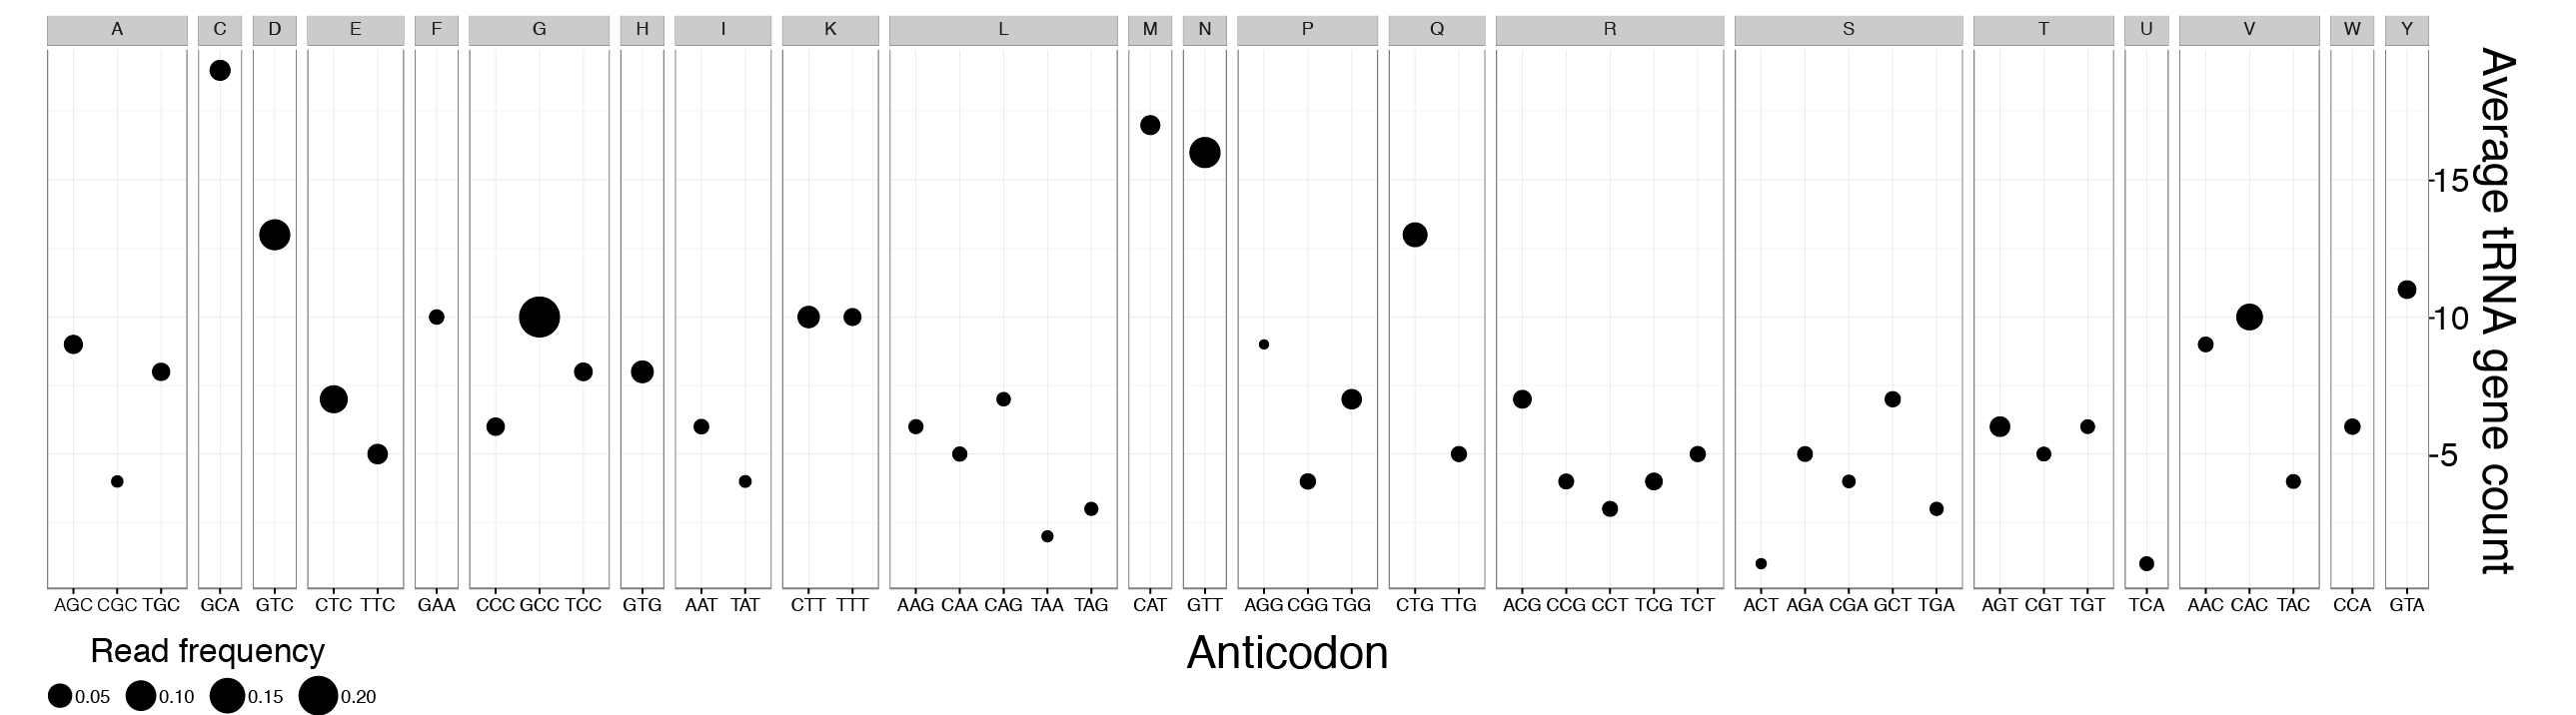
\includegraphics[width=\textwidth]{paper4D.png}%
\caption[Average gene count and relative frequency for each anticodon.] 
{\textbf{Average gene count and relative frequency for each anticodon.}
The gene count (mean of 4 replicates) is shown on the y-axis, anticodons on the x-axis; isotypes are indicated on the top. The area of each black disc is proportional to the fraction of reads mapping to all mature tRNAs for a given anticodon, normalized over all mature tRNAs for all anticodons.}
\centering
\label{discs}%
\end{figure}

\section{Mature tRNA abundance does not correlate with pre-tRNA abundance}
The next question that arose, was whether there was a correlation between individual pre-tRNAs and their mature transcripts. If that were the case, then one could conclude that tRNA maturation is a uniform process across all tRNAs that occurs without significant regulation on individual tRNAs.

Neither of the two techniques I employed showed any strong correlation between precursor and mature tRNA counts (R < 0.2; \textbf{\ref{supp4}A,B}). Our techniques can reproducibly quantify pre-tRNAs (\textbf{Fig. \ref{paper3}D}), and detect accumulation of pre-tRNA processing intermediates (see section \ref{clp1section}. Therefore, the observed lack of correlation is likely due to marked differences in the kinetics and dynamics of processing across tRNAs, and/or their pre-tRNA fragments' degradation, rather than due to experimental limitations in capturing processing intermediates. 

\begin{figure}[!h]%
\centering
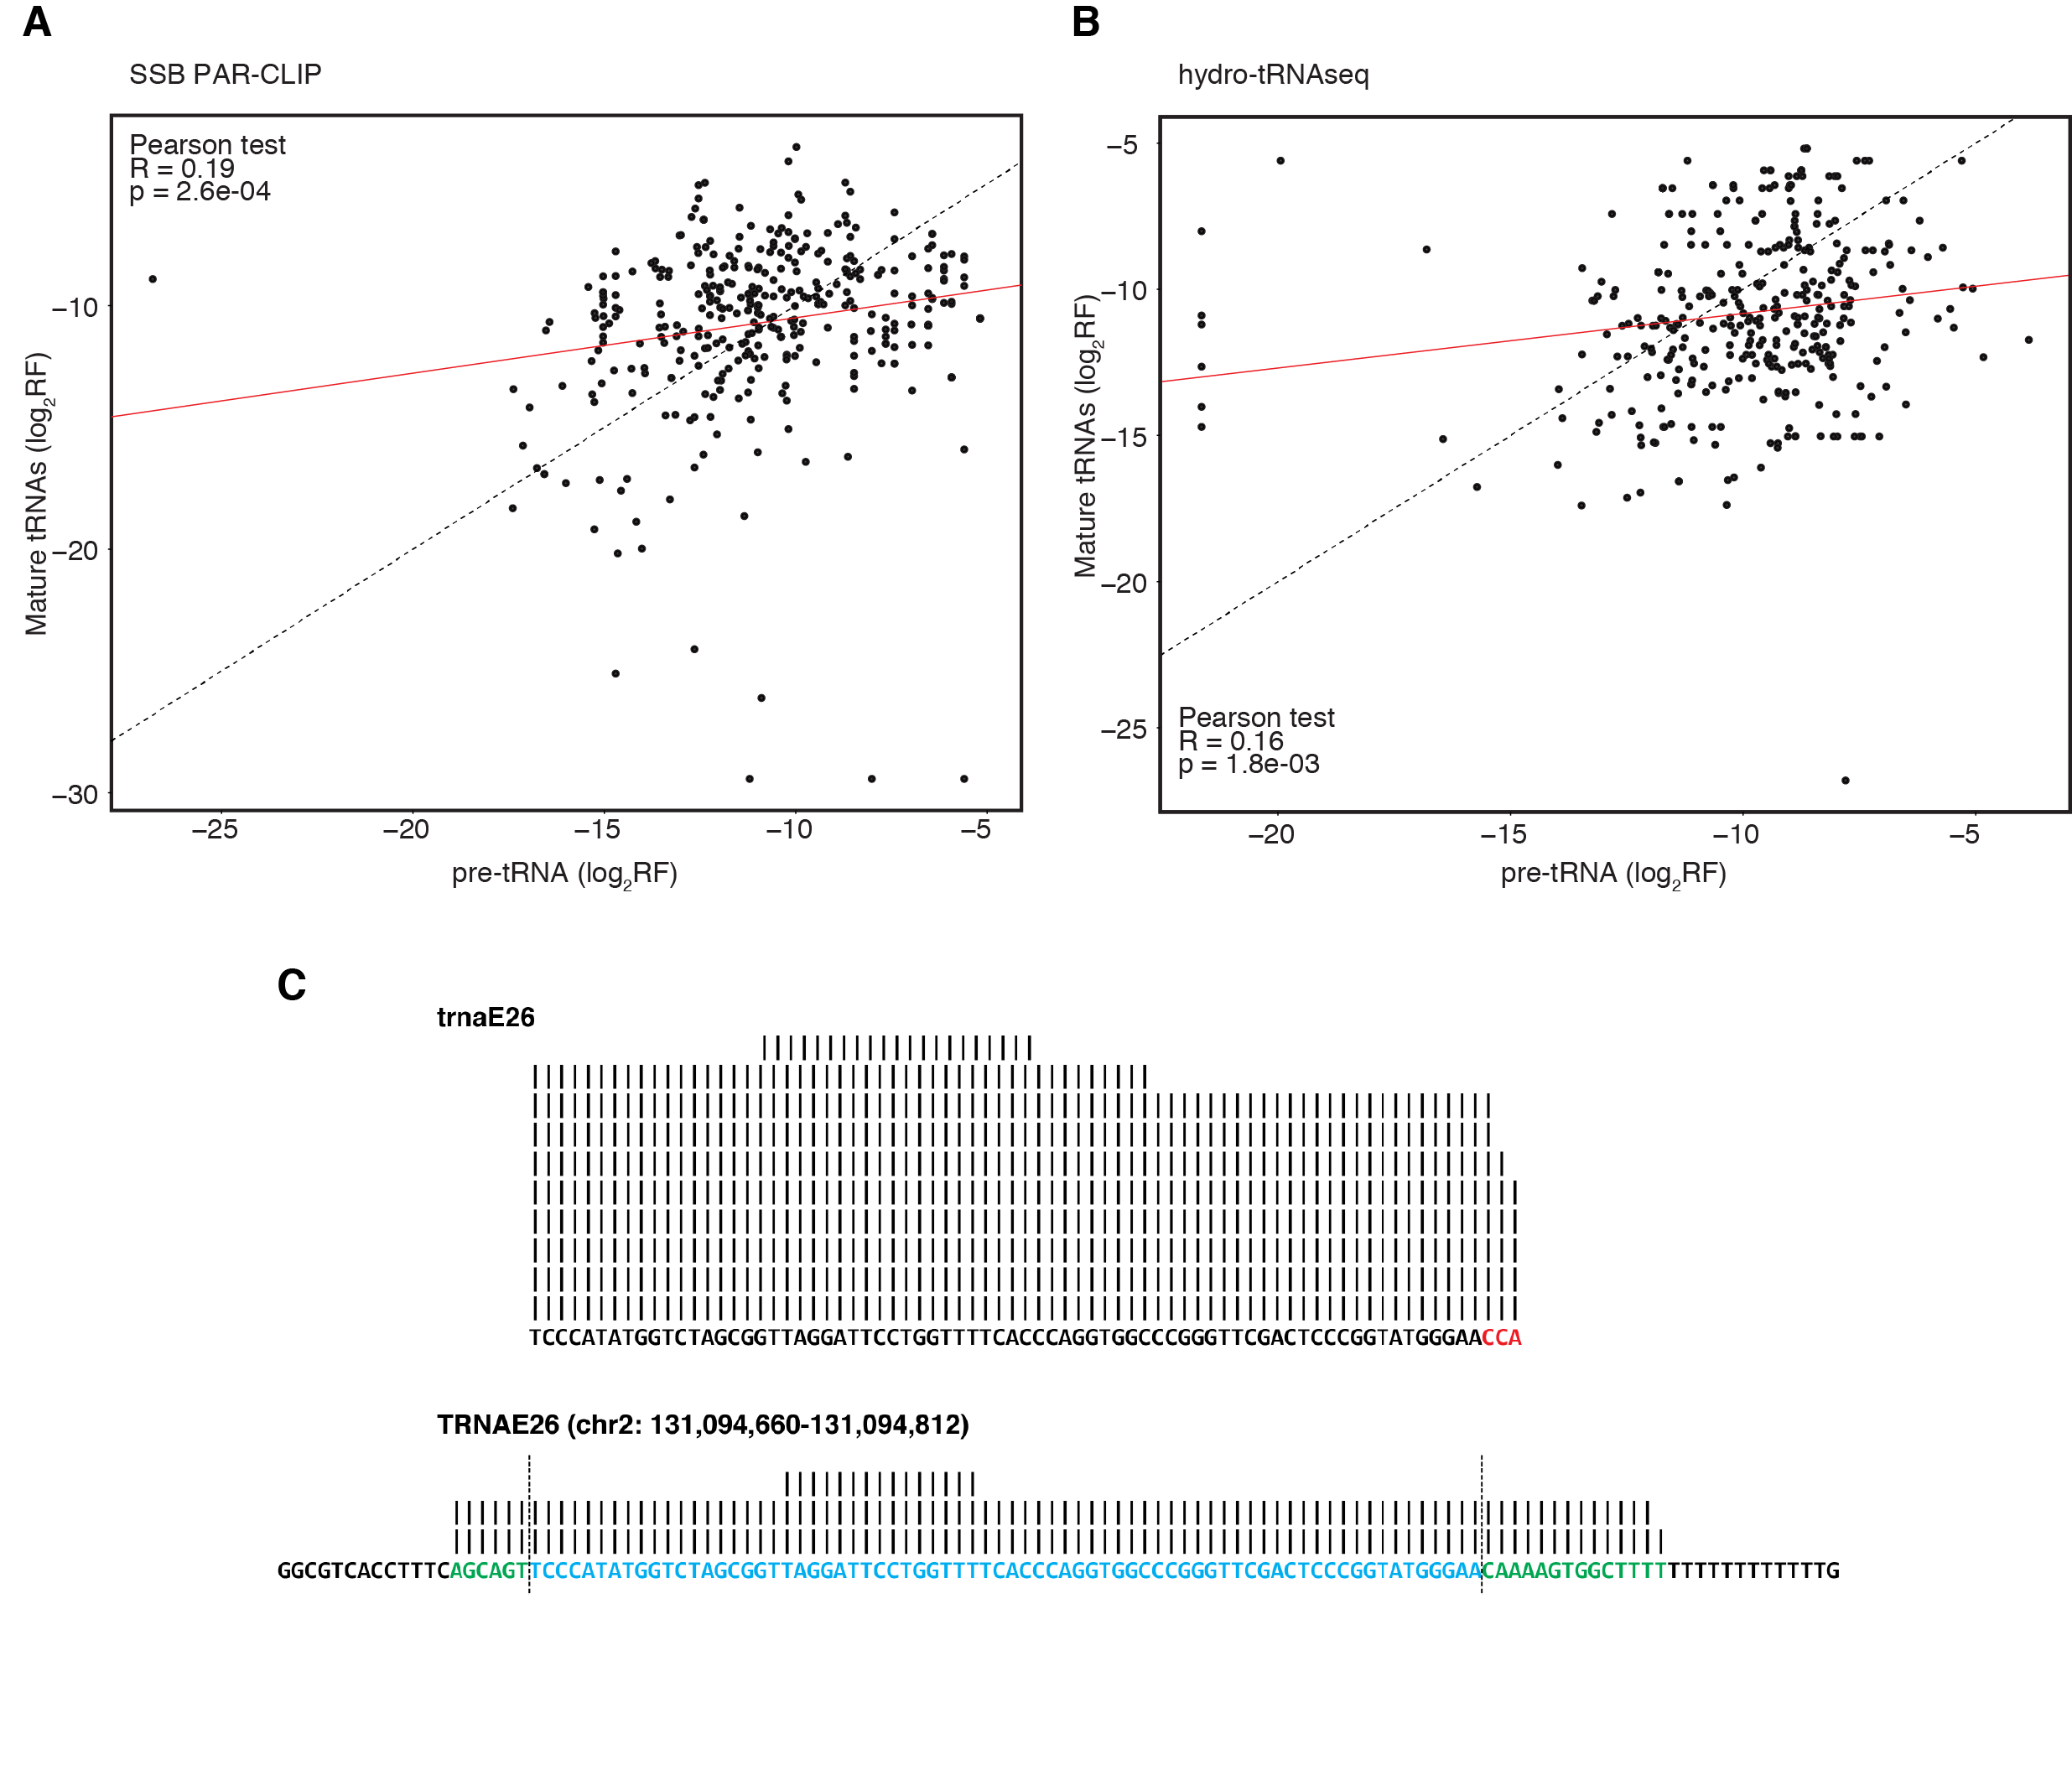
\includegraphics[width=\textwidth]{supp4b.png}%
\caption[Correlation between pre-tRNA and mature tRNA read frequencies.]
{
\textbf{Correlation between pre-tRNA and mature tRNA read frequencies.}
Correlation of relative read frequencies (log2-transformed) between pre-tRNA (x-axis) and mature tRNAs (y-axis) for SSB PAR-CLIP (A) and hydro-tRNAseq (B). Correlation was calculated using the Pearson test. Linear fit is shown in red. The y=x line (dotted) is shown for comparison. (C) Representative alignments of a mature tRNA (top) and its corresponding precursor (bottom). On the pre-tRNA reference, the mature sequence is labeled in blue, and the leader and trailer sequences in green, with their borders demarcated by vertical dotted lines. The post-transcriptionally added CCA tail is shown in red on the mature reference sequence. Vertical bars represent binned, log\sub{4}-transformed abundance. 
}
\centering
\label{supp4}%
\end{figure}

With respect to individual tRNAs, however, mature tRNA read counts were always higher than the respective pre-tRNA counts (\textbf{Fig. \ref{supp4}C}). This  suggests that tRNA processing is an efficient process across the tRNA spectrum, leading to prompt removal of intermediates and preventing accumulation of fragments that could possibly be toxic to the cells \cite{Hanada:2013bk}. 

\section{tRNA transcription initiation and termination}

Besides tRNA gene annotation and quantification, I realized that our approach could yield insights into POLR3 transcription initiation and termination, by paying attention to the length and characteristics of pre-tRNA leader and trailer sequences. To the best of my knowledge, such an analysis had not been previously performed on a transcriptome-wide level in human cells, even though elegant work had yielded valubale insights either \textit{in vitro} or \textit{in silico}, predominantly in yeast \cite{Maraia:2010kx,Arimbasseri:2013dg,Nielsen:2013be,Arimbasseri:2013by,Arimbasseri:2014hj,Arimbasseri:2015jg}.

\begin{figure}[!ht]%
\centering
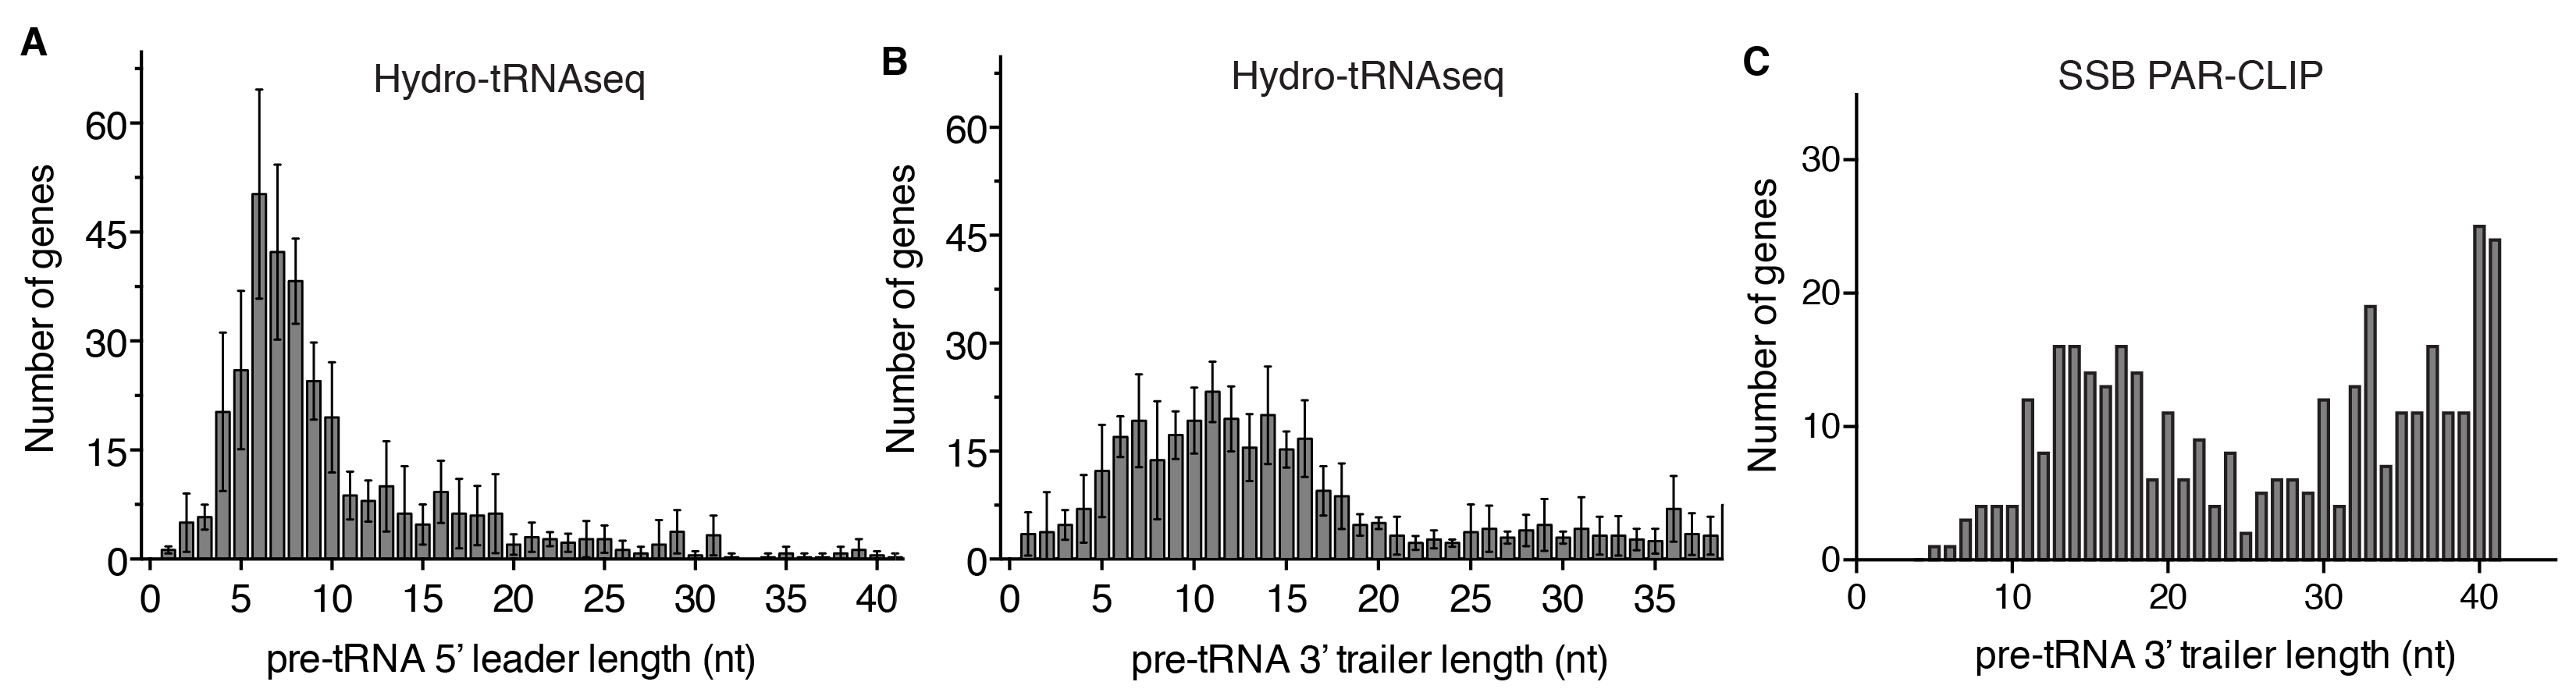
\includegraphics[width=\textwidth]{paper6.png}%
\caption[Boundaries of tRNA transcription initiation and termination.]
{\textbf{Boundaries of tRNA transcription initiation and termination.}
Histogram of the length distribution of precursor tRNA 5’ leaders (A) and 3’ trailers (B) detected by hydro-tRNAseq, and trailers detected by SSB PAR-CLIP (C). Mean $\pm$ standard deviation of four hydro-tRNAseq replicates shown in (A) and (B). Data from SSB PAR-CLIP replicate with RNase T1 shown in (C).}
\centering
\label{paper6}%
\end{figure}

Based on hydro-tRNAseq, I determined the median 5’ leader and 3’ trailer lengths to be 6 and 10 nt, respectively, with the trailer lengths showing a broader distribution, cengered around 12 nt (\textbf{Fig. \ref{paper6}A,B}). Interestingly, SSB PAR-CLIP revealed a subset of much longer trailers (\textbf{Fig. \ref{paper6}C}), suggesting that SSB PAR-CLIP captured the very initial steps of precursor tRNA processing, and accordingly that hydro-tRNAseq captures pre-tRNAs partially trimmed, either by ELAC2 (tRNase Z) or some other nuclease \cite{Phizicky:2010jf}.

I next focused on the POLR3 oligoU termination signals. Various reports in the past have focused on the oligoU requirements for transcription termination in different species \cite{Nielsen:2013be,Arimbasseri:2014hj}. SSB protected consistently a 3’ 4 to 5 nt oligoU stretch, which was also confirmed by hydro-tRNAseq (\textbf{Fig. \ref{paper6de}}). This is in agreement with previous \textit{in vitro} results \cite{Bayfield:2009cx,Stefano:1984wp,Teplova:2006dv}. We also addressed the proposed requirement for a stem-loop immediately upstream of the oligoU termination signal \cite{Nielsen:2013be}. Secondary structure predictions for the trailer sequences with documented sequence evidence in hydro-tRNAseq and SSB PAR-CLIP did not detect predicted stable stem-loop structures for approximately half of all pre-tRNAs (\textbf{Fig. \ref{supp5}}). This argued against a formal requirement for a stem-loop in the termination process of POLR3, at least on tRNA genes, in accordance with previous biochemical evidence \cite{Arimbasseri:2014hj}.


\begin{figure}[!ht]%
\centering
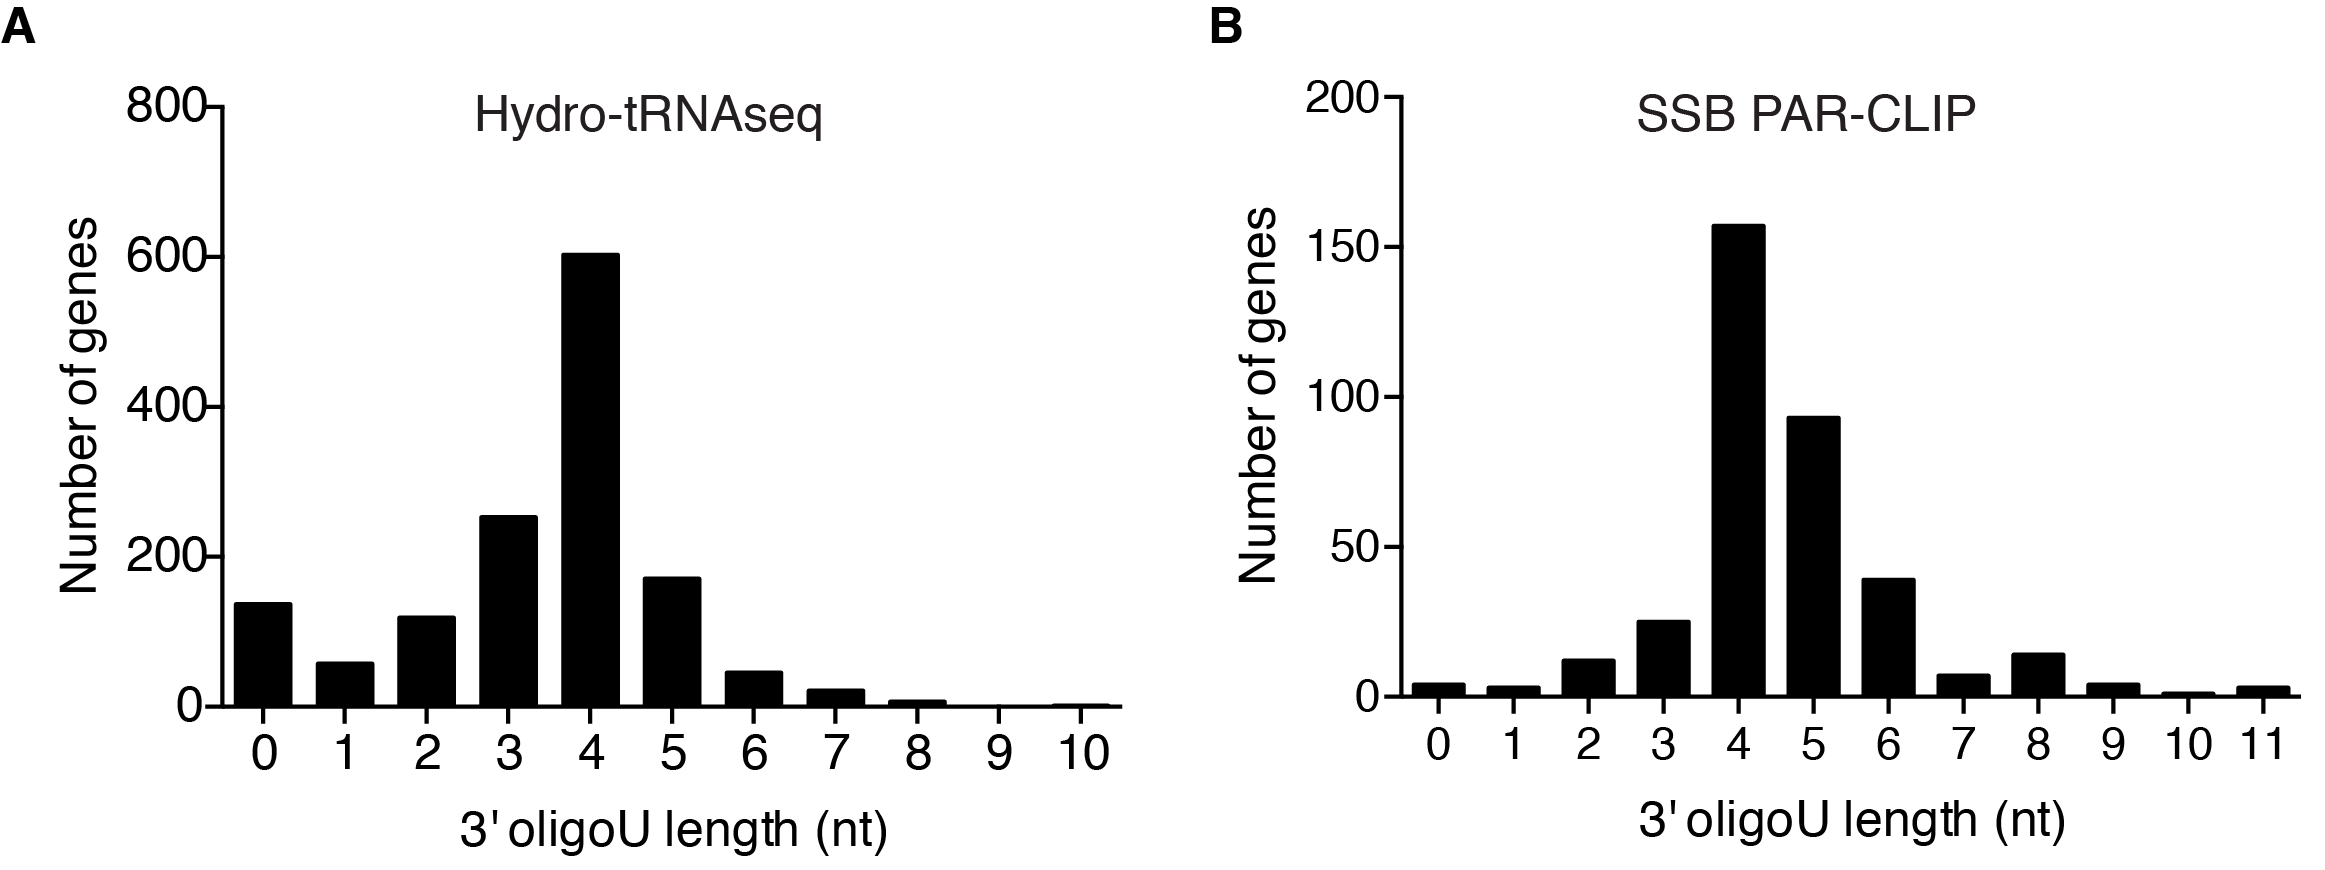
\includegraphics[width=\textwidth]{paper6de.png}%
\caption[POLR3 oligoU transcription termination signals]
{\textbf{POLR3 oligoU transcription termination signals.}
Histogram of the length distribution for the longest oligoU tract per pre-tRNA 3’ trailer detected by hydro-tRNAseq (A) (aggregate gene total of all replicates shown on the y-axis), and by SSB PAR-CLIP (B).}
\centering
\label{paper6de}%
\end{figure}

\begin{figure}[!ht]%
\centering
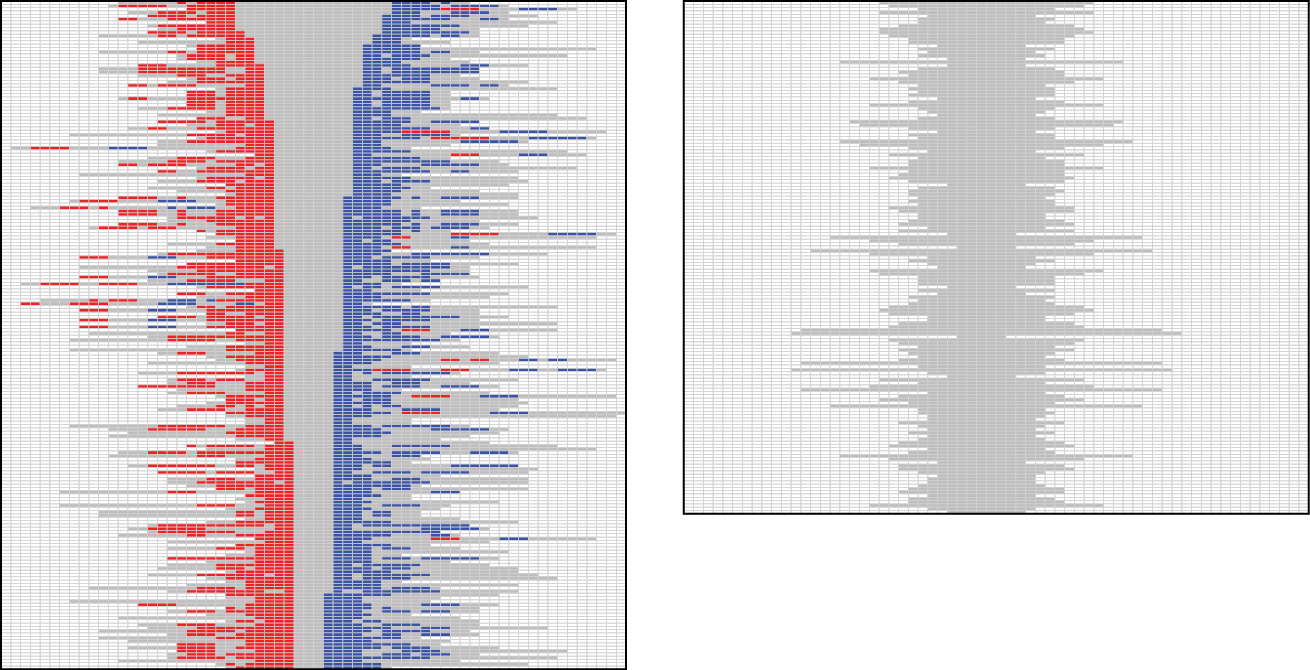
\includegraphics[width=\textwidth]{supp5.png}%
\caption[Predicted structures of precursor tRNA 3’ trailers with read evidence in SSB PAR-CLIP.]
{\textbf{Predicted structures of precursor tRNA 3’ trailers with read evidence in SSB PAR-CLIP.}
Every colored box indicates one nucleotide. Red and blue reflect the 5’ and 3’ parts of a duplex, respectively, whereas gray indicates non-basepaired nucleotides. About 1/2 of all tRNA trailers lack any predicted structure (right panel). The predicted stemloops do not have a uniform stem or loop length. Folding was performed using the Vienna folding package \cite{Lorenz:2011it}.}
\centering
\label{supp5}%
\end{figure}

\section{Ribonucleotide modifications}\label{modifications}

RT across modified nucleotide-containing RNA leads to errors in cognate deoxynucleotide incorporation, revealed by mismatches in sequence reads upon mapping to reference genomic sequence. Read coverage across regions with a high degree of modifications may result in incomplete or largely uneven coverage. Therefore, the compilation of my tRNA reference set, included the combination of all frequent mismatch signatures in all heavily modified positions. I reported the most frequently modified positions per tRNA gene (\textbf{Table \ref{mod_table}}), and computed the frequencies of every nucleoside change per position across all tRNA genes (the most common ones shown in \textbf{Fig. \ref{paper7a}}).

\twocolumn
{\tiny
\def\arraystretch{0.7}
\begin{center}
\tablefirsthead{
 \hline
 \multicolumn{1}{|l|}{\textbf{tRNA}} &
 \multicolumn{1}{l|}{\textbf{Position}} & 
 \multicolumn{1}{l|}{\textbf{Nucleoside}} & 
 \multicolumn{1}{l|}{\textbf{Read count}} \\
 \hline}
\tablehead{
 \hline
 \multicolumn{4}{|l|}{\textit{Continued from previous column}}\\
 \hline
 \multicolumn{1}{|l|}{\textbf{tRNA}} &
 \multicolumn{1}{l|}{\textbf{Position}} & 
 \multicolumn{1}{l|}{\textbf{Nucleoside}} & 
 \multicolumn{1}{l|}{\textbf{Read count}} \\
 \hline}
\tabletail{
 \hline
 \multicolumn{4}{|l|}{\textit{Continued on next column}} \\
 \hline}
\tablelasttail{\hline}
\bottomcaption[Positions resulting to modifications-induced mismatches.]{\textbf{Positions resulting to modifications-induced mismatches.} tRNA transcripts, the positions where modifications result in mismatches, and the read count corresponding to every observed nucleoside per position are shown.}
\begin{supertabular}{|l|r|c|r|}
\hline
 trnaA10 &        36 &          G &     25,957 \\
 trnaA10 &        36 &          T &      1,198 \\
 trnaA10 &        36 &          A &      2,206 \\
 trnaA10 &        36 &          C &         51 \\
 trnaA11 &        36 &          A &        100 \\
 trnaA11 &        36 &          T &         61 \\
 trnaA11 &        36 &          G &         95 \\
 trnaA13 &         6 &          C &      2,507 \\
 trnaA13 &         6 &          T &    175,171 \\
 trnaA13 &         6 &          A &      1,178 \\
 trnaA13 &         6 &          G &      6,873 \\
 trnaA13 &        10 &          G &    185,402 \\
 trnaA13 &        10 &          T &         39 \\
 trnaA13 &        10 &          A &        829 \\
 trnaA13 &        10 &          C &        136 \\
 trnaA13 &        16 &          C &      1,134 \\
 trnaA13 &        16 &          T &    189,165 \\
 trnaA13 &        16 &          G &      1,038 \\
 trnaA13 &        33 &          C &        112 \\
 trnaA13 &        33 &          A &        386 \\
 trnaA13 &        33 &          T &        110 \\
 trnaA13 &        33 &          G &    205,885 \\
 trnaA13 &        36 &          C &        559 \\
 trnaA13 &        36 &          T &     12,584 \\
 trnaA13 &        36 &          A &      4,747 \\
 trnaA13 &        36 &          G &    173,085 \\
 trnaA13 &        39 &          A &         30 \\
 trnaA13 &        39 &          T &      3,993 \\
 trnaA13 &        39 &          C &    172,312 \\
 trnaA13 &        45 &          T &        319 \\
 trnaA13 &        45 &          C &      1,202 \\
 trnaA13 &        45 &          G &     65,025 \\
 trnaA13 &        56 &          G &        126 \\
 trnaA13 &        56 &          T &          7 \\
 trnaA13 &        56 &          A &     36,136 \\
 trnaA13 &        56 &          C &         40 \\
 trnaA13 &        58 &          A &         13 \\
 trnaA13 &        58 &          T &     36,111 \\
 trnaA13 &        58 &          C &        117 \\
 trnaA13 &        58 &          G &          6 \\
 trnaA13 &        66 &          T &         62 \\
 trnaA13 &        66 &          A &     32,876 \\
 trnaA13 &        66 &          C &        684 \\
  trnaA2 &        34 &          G &     33,023 \\
  trnaA2 &        34 &          A &        206 \\
  trnaA2 &        34 &          T &         11 \\
  trnaA2 &        34 &          C &          9 \\
  trnaA2 &        37 &          A &      1,135 \\
  trnaA2 &        37 &          T &      9,316 \\
  trnaA2 &        37 &          C &        250 \\
  trnaA2 &        37 &          G &     23,009 \\
 trnaA23 &         5 &          G &     12,936 \\
 trnaA23 &         5 &          C &        593 \\
 trnaA23 &         5 &          T &        250 \\
 trnaA23 &         5 &          A &    277,684 \\
 trnaA23 &        33 &          C &    206,326 \\
 trnaA23 &        33 &          T &    215,944 \\
 trnaA23 &        33 &          A &        126 \\
 trnaA23 &        36 &          A &      9,456 \\
 trnaA23 &        36 &          T &     18,956 \\
 trnaA23 &        36 &          G &    415,552 \\
 trnaA23 &        46 &          G &        992 \\
 trnaA23 &        46 &          A &        366 \\
 trnaA23 &        46 &          T &    102,084 \\
 trnaA23 &        46 &          C &    145,919 \\
 trnaA23 &        67 &          C &      2,990 \\
 trnaA23 &        67 &          T &    145,047 \\
 trnaA23 &        67 &          A &         16 \\
 trnaA28 &        33 &          A &         98 \\
 trnaA28 &        33 &          T &         50 \\
 trnaA28 &        33 &          C &      1,180 \\
 trnaA28 &        33 &          G &     38,349 \\
 trnaA28 &        36 &          G &     26,060 \\
 trnaA28 &        36 &          C &         54 \\
 trnaA28 &        36 &          A &        922 \\
 trnaA28 &        36 &          T &      1,098 \\
 trnaA28 &        45 &          T &        478 \\
 trnaA28 &        45 &          A &         19 \\
 trnaA28 &        45 &          C &         21 \\
 trnaA28 &        45 &          G &      7,579 \\
  trnaA3 &        34 &          C &         25 \\
  trnaA3 &        34 &          A &        205 \\
  trnaA3 &        34 &          T &         26 \\
  trnaA3 &        34 &          G &    101,158 \\
  trnaA3 &        37 &          G &     79,503 \\
  trnaA3 &        37 &          C &        673 \\
  trnaA3 &        37 &          T &     28,670 \\
  trnaA3 &        37 &          A &      2,886 \\
 trnaA32 &        36 &          C &        155 \\
 trnaA32 &        36 &          A &    107,454 \\
 trnaA32 &        36 &          T &        254 \\
 trnaA32 &        36 &          G &      7,740 \\
 trnaA32 &        45 &          G &     74,872 \\
 trnaA32 &        45 &          C &      3,688 \\
 trnaA32 &        45 &          A &         75 \\
 trnaA32 &        45 &          T &      1,610 \\
 trnaA34 &        33 &          G &     33,690 \\
 trnaA34 &        33 &          C &         15 \\
 trnaA34 &        33 &          A &        219 \\
 trnaA34 &        33 &          T &         20 \\
 trnaA34 &        36 &          G &     27,770 \\
 trnaA34 &        36 &          T &      2,594 \\
 trnaA34 &        36 &          A &      1,468 \\
 trnaA34 &        36 &          C &        128 \\
  trnaA6 &        33 &          G &      2,435 \\
  trnaA6 &        33 &          C &          7 \\
  trnaA6 &        33 &          T &          6 \\
  trnaA6 &        33 &          A &      5,790 \\
  trnaA6 &        36 &          G &      3,318 \\
  trnaA6 &        36 &          C &         31 \\
  trnaA6 &        36 &          A &      4,344 \\
  trnaA6 &        36 &          T &        380 \\
  trnaA7 &        33 &          A &      1,183 \\
  trnaA7 &        33 &          T &      1,892 \\
  trnaA7 &        33 &          C &      1,117 \\
  trnaA7 &        33 &          G &     27,108 \\
  trnaA7 &        36 &          G &     20,964 \\
  trnaA7 &        36 &          T &     12,246 \\
  trnaA7 &        36 &          A &      3,841 \\
  trnaA7 &        36 &          C &        594 \\
 trnaC10 &         6 &          G &     15,648 \\
 trnaC10 &         6 &          C &    101,951 \\
 trnaC10 &         6 &          T &      2,423 \\
 trnaC10 &         6 &          A &      5,244 \\
 trnaC10 &        16 &          G &     26,551 \\
 trnaC10 &        16 &          C &      2,047 \\
 trnaC10 &        16 &          A &      1,356 \\
 trnaC10 &        16 &          T &    117,667 \\
 trnaC11 &        16 &          C &         10 \\
 trnaC11 &        16 &          T &        783 \\
 trnaC11 &        16 &          G &      4,230 \\
 trnaC11 &        44 &          A &         82 \\
 trnaC11 &        44 &          T &         10 \\
 trnaC11 &        44 &          G &        803 \\
 trnaC14 &         6 &          G &      4,417 \\
 trnaC14 &         6 &          C &      2,002 \\
 trnaC14 &         6 &          A &        762 \\
 trnaC14 &         6 &          T &     92,027 \\
 trnaC14 &        57 &          A &     47,747 \\
 trnaC14 &        57 &          T &      5,006 \\
 trnaC14 &        57 &          C &        391 \\
 trnaC14 &        57 &          G &      6,331 \\
 trnaC21 &        42 &          G &     33,541 \\
 trnaC21 &        42 &          C &         73 \\
 trnaC21 &        42 &          A &      7,594 \\
 trnaC21 &        42 &          T &        181 \\
 trnaC24 &         6 &          G &      5,664 \\
 trnaC24 &         6 &          T &     95,339 \\
 trnaC24 &         6 &          A &      1,284 \\
 trnaC24 &         6 &          C &     16,078 \\
 trnaC24 &        57 &          T &      9,354 \\
 trnaC24 &        57 &          A &    139,890 \\
 trnaC24 &        57 &          C &        339 \\
 trnaC24 &        57 &          G &      9,511 \\
  trnaC7 &        57 &          G &      1,048 \\
  trnaC7 &        57 &          T &        931 \\
  trnaC7 &        57 &          A &     25,533 \\
  trnaC7 &        57 &          C &         20 \\
 trnaD10 &         9 &          G &        813 \\
 trnaD10 &         9 &          T &        304 \\
 trnaD10 &         9 &          A &    118,147 \\
 trnaD10 &         9 &          C &         89 \\
 trnaD10 &        53 &          C &     19,831 \\
 trnaD10 &        53 &          A &      1,716 \\
 trnaD10 &        53 &          T &    472,250 \\
 trnaD10 &        53 &          G &     45,707 \\
 trnaD10 &        56 &          G &    367,491 \\
 trnaD10 &        56 &          C &      1,093 \\
 trnaD10 &        56 &          T &        846 \\
 trnaD10 &        56 &          A &    144,309 \\
 trnaD10 &        57 &          G &      2,914 \\
 trnaD10 &        57 &          T &     16,380 \\
 trnaD10 &        57 &          A &    492,772 \\
 trnaD10 &        57 &          C &        791 \\
  trnaD9 &        24 &          C &        468 \\
  trnaD9 &        24 &          A &      4,669 \\
  trnaD9 &        24 &          T &      1,114 \\
  trnaD9 &        24 &          G &      2,101 \\
  trnaD9 &        31 &          C &     91,720 \\
  trnaD9 &        31 &          T &      2,596 \\
  trnaD9 &        31 &          A &        953 \\
  trnaD9 &        31 &          G &      2,238 \\
  trnaD9 &        56 &          A &    114,699 \\
  trnaD9 &        56 &          T &        609 \\
  trnaD9 &        56 &          C &        858 \\
  trnaD9 &        56 &          G &  1,051,388 \\
  trnaD9 &        57 &          G &      9,918 \\
  trnaD9 &        57 &          A &  1,095,714 \\
  trnaD9 &        57 &          T &     59,596 \\
  trnaD9 &        57 &          C &      2,145 \\
  trnaE5 &         9 &          G &    913,314 \\
  trnaE5 &         9 &          A &      1,503 \\
  trnaE5 &         9 &          T &      1,502 \\
  trnaE5 &         9 &          C &      1,330 \\
  trnaE5 &        19 &          G &        668 \\
  trnaE5 &        19 &          A &        198 \\
  trnaE5 &        19 &          T &  1,171,172 \\
  trnaE5 &        19 &          C &      3,141 \\
  trnaE5 &        24 &          G &     18,086 \\
  trnaE5 &        24 &          A &  1,368,739 \\
  trnaE5 &        24 &          T &      2,320 \\
  trnaE5 &        24 &          C &      2,252 \\
  trnaE5 &        27 &          G &      4,750 \\
  trnaE5 &        27 &          T &     27,560 \\
  trnaE5 &        27 &          A &      3,180 \\
  trnaE5 &        27 &          C &  1,490,638 \\
  trnaE5 &        34 &          C &  1,948,790 \\
  trnaE5 &        34 &          A &      1,036 \\
  trnaE5 &        34 &          T &     45,989 \\
  trnaE5 &        34 &          G &      1,246 \\
  trnaE5 &        53 &          G &     46,498 \\
  trnaE5 &        53 &          A &      3,717 \\
  trnaE5 &        53 &          T &  1,971,842 \\
  trnaE5 &        53 &          C &     16,977 \\
  trnaE5 &        57 &          G &     27,513 \\
  trnaE5 &        57 &          C &     12,646 \\
  trnaE5 &        57 &          A &  1,784,527 \\
  trnaE5 &        57 &          T &    163,808 \\
  trnaE7 &         6 &          G &        442 \\
  trnaE7 &         6 &          T &    224,221 \\
  trnaE7 &         6 &          A &        428 \\
  trnaE7 &         6 &          C &    622,013 \\
  trnaE7 &         9 &          G &    925,734 \\
  trnaE7 &         9 &          A &      1,682 \\
  trnaE7 &         9 &          T &      3,498 \\
  trnaE7 &         9 &          C &      1,570 \\
  trnaE7 &        34 &          G &      7,239 \\
  trnaE7 &        34 &          C &     63,597 \\
  trnaE7 &        34 &          T &  1,701,031 \\
  trnaE7 &        34 &          A &      5,025 \\
  trnaE7 &        44 &          A &      3,111 \\
  trnaE7 &        44 &          T &    209,800 \\
  trnaE7 &        44 &          C &  1,445,839 \\
  trnaE7 &        44 &          G &      8,730 \\
  trnaE7 &        66 &          C &         36 \\
  trnaE7 &        66 &          T &      1,122 \\
  trnaE7 &        66 &          A &    154,605 \\
  trnaE7 &        66 &          G &  1,018,843 \\
  trnaF5 &         6 &          A &      1,703 \\
  trnaF5 &         6 &          C &         36 \\
  trnaF5 &         6 &          G &      1,587 \\
  trnaF5 &        47 &          G &        783 \\
  trnaF5 &        47 &          T &     17,158 \\
  trnaF5 &        47 &          C &      2,431 \\
  trnaF5 &        57 &          A &      3,199 \\
  trnaF5 &        57 &          G &     16,069 \\
 trnaG15 &         5 &          G &    983,413 \\
 trnaG15 &         5 &          T &    477,119 \\
 trnaG15 &         5 &          A &      2,009 \\
 trnaG15 &         5 &          C &      5,058 \\
 trnaG15 &        45 &          G &  1,455,904 \\
 trnaG15 &        45 &          T &      3,715 \\
 trnaG15 &        45 &          A &    131,627 \\
 trnaG15 &        45 &          C &     10,529 \\
 trnaG15 &        56 &          C &      2,347 \\
 trnaG15 &        56 &          T &    137,083 \\
 trnaG15 &        56 &          A &    802,531 \\
 trnaG15 &        56 &          G &     23,277 \\
 trnaG15 &        66 &          G &         13 \\
 trnaG15 &        66 &          A &    556,240 \\
 trnaG15 &        66 &          C &    353,038 \\
 trnaH11 &         5 &          A &        687 \\
 trnaH11 &         5 &          T &      1,239 \\
 trnaH11 &         5 &          C &        243 \\
 trnaH11 &         5 &          G &      9,794 \\
 trnaH11 &        33 &          A &        729 \\
 trnaH11 &        33 &          T &    897,345 \\
 trnaH11 &        33 &          C &      5,452 \\
 trnaH11 &        33 &          G &      8,216 \\
 trnaH11 &        58 &          G &     20,143 \\
 trnaH11 &        58 &          C &        260 \\
 trnaH11 &        58 &          T &     27,065 \\
 trnaH11 &        58 &          A &    870,683 \\
  trnaI5 &        27 &          G &      2,177 \\
  trnaI5 &        27 &          T &      1,830 \\
  trnaI5 &        35 &          G &     32,621 \\
  trnaI5 &        35 &          A &        107 \\
  trnaI5 &        60 &          A &      3,085 \\
  trnaI5 &        60 &          T &     36,960 \\
  trnaI5 &        69 &          G &     36,009 \\
  trnaI5 &        69 &          T &      2,962 \\
  trnaI9 &        27 &          T &      2,220 \\
  trnaI9 &        27 &          A &         90 \\
  trnaI9 &        27 &          C &         79 \\
  trnaI9 &        27 &          G &     18,350 \\
  trnaI9 &        35 &          G &     54,591 \\
  trnaI9 &        35 &          T &          7 \\
  trnaI9 &        35 &          A &        189 \\
  trnaI9 &        59 &          G &      1,438 \\
  trnaI9 &        59 &          C &        229 \\
  trnaI9 &        59 &          T &      3,282 \\
  trnaI9 &        59 &          A &     43,060 \\
  trnaI9 &        60 &          G &          9 \\
  trnaI9 &        60 &          C &         27 \\
  trnaI9 &        60 &          A &      3,213 \\
  trnaI9 &        60 &          T &     44,664 \\
  trnaI9 &        69 &          T &      5,705 \\
  trnaI9 &        69 &          C &         92 \\
  trnaI9 &        69 &          G &     38,915 \\
  trnaK1 &        54 &          G &     12,329 \\
  trnaK1 &        54 &          T &    529,905 \\
  trnaK1 &        54 &          A &      2,946 \\
  trnaK1 &        54 &          C &      7,353 \\
  trnaK1 &        58 &          C &      1,742 \\
  trnaK1 &        58 &          T &     22,380 \\
  trnaK1 &        58 &          A &    435,401 \\
  trnaK1 &        58 &          G &     81,542 \\
  trnaL1 &        27 &          G &     52,413 \\
  trnaL1 &        27 &          T &      4,682 \\
  trnaL1 &        27 &          A &      2,091 \\
  trnaL1 &        27 &          C &        717 \\
  trnaL1 &        35 &          C &         21 \\
  trnaL1 &        35 &          T &      2,285 \\
  trnaL1 &        35 &          A &        546 \\
  trnaL1 &        35 &          G &     68,859 \\
  trnaL1 &        67 &          G &      1,793 \\
  trnaL1 &        67 &          C &        221 \\
  trnaL1 &        67 &          A &     55,644 \\
  trnaL1 &        67 &          T &      2,456 \\
 trnaL15 &        10 &          G &     12,159 \\
 trnaL15 &        10 &          T &         13 \\
 trnaL15 &        10 &          A &         12 \\
 trnaL15 &        10 &          C &        863 \\
 trnaL15 &        12 &          G &          5 \\
 trnaL15 &        12 &          T &        647 \\
 trnaL15 &        12 &          A &          2 \\
 trnaL15 &        12 &          C &     12,503 \\
 trnaL15 &        27 &          C &         80 \\
 trnaL15 &        27 &          A &        316 \\
 trnaL15 &        27 &          T &        720 \\
 trnaL15 &        27 &          G &     12,945 \\
  trnaL4 &        27 &          G &     21,789 \\
  trnaL4 &        27 &          T &        812 \\
  trnaL4 &        35 &          G &     21,913 \\
  trnaL4 &        35 &          A &        202 \\
  trnaL4 &        67 &          T &        206 \\
  trnaL4 &        67 &          A &      3,302 \\
  trnaL4 &        67 &          G &        176 \\
  trnaL5 &        51 &          G &      4,824 \\
  trnaL5 &        51 &          C &     24,212 \\
  trnaL5 &        51 &          T &     19,749 \\
  trnaL5 &        51 &          A &      2,548 \\
  trnaM1 &         9 &          G &     85,934 \\
  trnaM1 &         9 &          C &      6,935 \\
  trnaM1 &         9 &          A &      5,666 \\
  trnaM1 &         9 &          T &     23,834 \\
  trnaM1 &        57 &          A &    312,240 \\
  trnaM1 &        57 &          T &     18,020 \\
  trnaM1 &        57 &          C &      1,202 \\
  trnaM1 &        57 &          G &     12,797 \\
 trnaM13 &        20 &          G &        779 \\
 trnaM13 &        20 &          T &     20,233 \\
 trnaM13 &        20 &          A &        393 \\
 trnaM13 &        20 &          C &      2,235 \\
 trnaM13 &        26 &          A &        802 \\
 trnaM13 &        26 &          T &      3,204 \\
 trnaM13 &        26 &          C &        113 \\
 trnaM13 &        26 &          G &     34,706 \\
 trnaM13 &        58 &          G &      6,039 \\
 trnaM13 &        58 &          A &    372,150 \\
 trnaM13 &        58 &          T &      7,682 \\
 trnaM13 &        58 &          C &        894 \\
 trnaM13 &        59 &          G &    141,279 \\
 trnaM13 &        59 &          C &      1,112 \\
 trnaM13 &        59 &          T &    243,802 \\
 trnaM13 &        59 &          A &        273 \\
  trnaN1 &        27 &          C &      5,696 \\
  trnaN1 &        27 &          A &      5,664 \\
  trnaN1 &        27 &          T &    133,510 \\
  trnaN1 &        27 &          G &    250,204 \\
  trnaN1 &        59 &          T &     79,049 \\
  trnaN1 &        59 &          A &    827,307 \\
  trnaN1 &        59 &          C &      4,741 \\
  trnaN1 &        59 &          G &    127,829 \\
 trnaN14 &        27 &          G &    102,061 \\
 trnaN14 &        27 &          A &      4,021 \\
 trnaN14 &        27 &          T &     21,768 \\
 trnaN14 &        27 &          C &      1,392 \\
 trnaN14 &        59 &          G &      7,434 \\
 trnaN14 &        59 &          C &        706 \\
 trnaN14 &        59 &          A &    151,684 \\
 trnaN14 &        59 &          T &      9,968 \\
 trnaP10 &        19 &          C &      4,621 \\
 trnaP10 &        19 &          A &      2,631 \\
 trnaP10 &        19 &          T &    411,265 \\
 trnaP10 &        19 &          G &     45,430 \\
 trnaP10 &        33 &          C &    183,783 \\
 trnaP10 &        33 &          T &     89,056 \\
 trnaP10 &        33 &          A &      1,332 \\
 trnaP10 &        33 &          G &    461,368 \\
 trnaP10 &        39 &          G &      3,517 \\
 trnaP10 &        39 &          T &     81,988 \\
 trnaP10 &        39 &          A &        972 \\
 trnaP10 &        39 &          C &    592,210 \\
  trnaQ1 &        56 &          C &      1,480 \\
  trnaQ1 &        56 &          A &  1,768,755 \\
  trnaQ1 &        56 &          T &        617 \\
  trnaQ1 &        56 &          G &      8,734 \\
  trnaQ1 &        57 &          G &     29,151 \\
  trnaQ1 &        57 &          T &      4,802 \\
  trnaQ1 &        57 &          A &  1,692,736 \\
  trnaQ1 &        57 &          C &      2,268 \\
  trnaQ1 &        58 &          G &     23,220 \\
  trnaQ1 &        58 &          T &      1,535 \\
  trnaQ1 &        58 &          A &  1,685,855 \\
  trnaQ1 &        58 &          C &      7,182 \\
  trnaQ2 &        32 &          A &        147 \\
  trnaQ2 &        32 &          T &        391 \\
  trnaQ2 &        32 &          C &    220,622 \\
  trnaQ2 &        32 &          G &     38,543 \\
 trnaR10 &        19 &          G &        880 \\
 trnaR10 &        19 &          C &         25 \\
 trnaR10 &        19 &          T &         77 \\
 trnaR10 &        19 &          A &     66,484 \\
 trnaR10 &        34 &          T &         42 \\
 trnaR10 &        34 &          A &      4,136 \\
 trnaR10 &        34 &          C &         51 \\
 trnaR10 &        34 &          G &    115,152 \\
 trnaR10 &        58 &          G &      4,908 \\
 trnaR10 &        58 &          A &     68,405 \\
 trnaR10 &        58 &          T &      2,439 \\
 trnaR10 &        58 &          C &        227 \\
  trnaR2 &        19 &          G &      6,415 \\
  trnaR2 &        19 &          T &        133 \\
  trnaR2 &        19 &          A &    122,886 \\
  trnaR2 &        19 &          C &         97 \\
  trnaR2 &        34 &          G &    238,519 \\
  trnaR2 &        34 &          C &        203 \\
  trnaR2 &        34 &          A &      6,830 \\
  trnaR2 &        34 &          T &        160 \\
  trnaR2 &        58 &          G &     11,883 \\
  trnaR2 &        58 &          A &    152,011 \\
  trnaR2 &        58 &          T &      4,470 \\
  trnaR2 &        58 &          C &        653 \\
 trnaR22 &        58 &          C &      1,653 \\
 trnaR22 &        58 &          T &     28,134 \\
 trnaR22 &        58 &          A &    325,452 \\
 trnaR22 &        58 &          G &     53,856 \\
 trnaR25 &        32 &          C &    164,623 \\
 trnaR25 &        32 &          T &     25,406 \\
 trnaR25 &        32 &          A &        171 \\
 trnaR25 &        32 &          G &        161 \\
 trnaR25 &        34 &          G &         78 \\
 trnaR25 &        34 &          C &     41,819 \\
 trnaR25 &        34 &          T &    187,213 \\
 trnaR25 &        34 &          A &        115 \\
 trnaR25 &        58 &          C &      1,903 \\
 trnaR25 &        58 &          A &    242,429 \\
 trnaR25 &        58 &          T &     29,879 \\
 trnaR25 &        58 &          G &     51,224 \\
  trnaR4 &        37 &          C &      2,958 \\
  trnaR4 &        37 &          T &     10,499 \\
  trnaR4 &        37 &          A &      2,141 \\
  trnaR4 &        37 &          G &    384,444 \\
  trnaR4 &        58 &          G &     54,001 \\
  trnaR4 &        58 &          A &    392,684 \\
  trnaR4 &        58 &          T &     30,994 \\
  trnaR4 &        58 &          C &      1,602 \\
  trnaR7 &        58 &          A &    150,051 \\
  trnaR7 &        58 &          T &      5,083 \\
  trnaR7 &        58 &          C &        537 \\
  trnaR7 &        58 &          G &      3,895 \\
 trnaS16 &        52 &          C &      6,033 \\
 trnaS16 &        52 &          A &      2,966 \\
 trnaS16 &        52 &          G &      5,330 \\
 trnaT14 &        35 &          G &     87,515 \\
 trnaT14 &        35 &          C &        513 \\
 trnaT14 &        35 &          T &        326 \\
 trnaT14 &        35 &          A &        159 \\
 trnaT14 &        59 &          G &      3,635 \\
 trnaT14 &        59 &          T &     10,441 \\
 trnaT14 &        59 &          A &    108,722 \\
 trnaT14 &        59 &          C &        746 \\
  trnaT2 &        26 &          C &        209 \\
  trnaT2 &        26 &          A &     16,122 \\
  trnaT2 &        26 &          T &         20 \\
  trnaT2 &        26 &          G &         61 \\
  trnaT2 &        58 &          G &         39 \\
  trnaT2 &        58 &          T &        833 \\
  trnaT2 &        58 &          A &      5,715 \\
  trnaT2 &        58 &          C &         18 \\
 trnaT21 &        35 &          A &         19 \\
 trnaT21 &        35 &          T &        490 \\
 trnaT21 &        35 &          C &         48 \\
 trnaT21 &        35 &          G &      9,748 \\
 trnaT21 &        59 &          A &     10,638 \\
 trnaT21 &        59 &          T &        240 \\
 trnaT21 &        59 &          C &         59 \\
 trnaT21 &        59 &          G &      1,403 \\
  trnaT4 &        35 &          C &        538 \\
  trnaT4 &        35 &          T &      2,319 \\
  trnaT4 &        35 &          A &        472 \\
  trnaT4 &        35 &          G &    210,546 \\
  trnaT4 &        59 &          G &     18,477 \\
  trnaT4 &        59 &          C &      1,524 \\
  trnaT4 &        59 &          T &     21,160 \\
  trnaT4 &        59 &          A &    325,542 \\
  trnaT4 &        70 &          G &      3,512 \\
  trnaT4 &        70 &          C &      4,114 \\
  trnaT4 &        70 &          A &      1,371 \\
  trnaT4 &        70 &          T &    345,239 \\
  trnaU1 &        28 &          C &         39 \\
  trnaU1 &        28 &          A &         15 \\
  trnaU1 &        28 &          T &      3,002 \\
  trnaU1 &        28 &          G &         97 \\
  trnaU1 &        64 &          A &         61 \\
  trnaU1 &        64 &          T &      7,513 \\
  trnaU1 &        64 &          C &        112 \\
  trnaU1 &        64 &          G &        385 \\
  trnaU1 &        71 &          T &        706 \\
  trnaU1 &        71 &          A &      6,359 \\
  trnaU1 &        71 &          C &         10 \\
  trnaU1 &        71 &          G &         67 \\
 trnaV12 &        34 &          G &     10,863 \\
 trnaV12 &        34 &          C &     11,001 \\
 trnaV12 &        34 &          A &        122 \\
 trnaV12 &        34 &          T &        221 \\
 trnaV12 &        67 &          G &     59,792 \\
 trnaV12 &        67 &          A &      1,838 \\
 trnaV12 &        67 &          T &        344 \\
 trnaV12 &        67 &          C &        376 \\
  trnaV2 &        19 &          G &      4,257 \\
  trnaV2 &        19 &          C &     10,750 \\
  trnaV2 &        19 &          A &      1,121 \\
  trnaV2 &        19 &          T &    889,930 \\
  trnaV2 &        20 &          G &        202 \\
  trnaV2 &        20 &          C &    361,327 \\
  trnaV2 &        20 &          T &    546,333 \\
  trnaV2 &        20 &          A &        678 \\
  trnaV2 &        26 &          G &    873,859 \\
  trnaV2 &        26 &          A &      5,271 \\
  trnaV2 &        26 &          T &     46,502 \\
  trnaV2 &        26 &          C &      7,245 \\
  trnaV2 &        34 &          C &    445,948 \\
  trnaV2 &        34 &          A &      1,387 \\
  trnaV2 &        34 &          T &      2,668 \\
  trnaV2 &        34 &          G &    948,953 \\
  trnaV2 &        58 &          G &     67,711 \\
  trnaV2 &        58 &          A &    946,402 \\
  trnaV2 &        58 &          T &    101,713 \\
  trnaV2 &        58 &          C &      5,446 \\
 trnaV27 &        26 &          G &    416,151 \\
 trnaV27 &        26 &          C &      3,461 \\
 trnaV27 &        26 &          T &     18,759 \\
 trnaV27 &        26 &          A &      1,627 \\
 trnaV27 &        58 &          G &     13,799 \\
 trnaV27 &        58 &          C &      1,270 \\
 trnaV27 &        58 &          T &     21,819 \\
 trnaV27 &        58 &          A &    168,700 \\
  trnaV8 &        34 &          A &        471 \\
  trnaV8 &        34 &          T &        525 \\
  trnaV8 &        34 &          C &     47,407 \\
  trnaV8 &        34 &          G &     84,016 \\
  trnaW2 &        70 &          C &        708 \\
  trnaW2 &        70 &          A &        165 \\
  trnaW2 &        70 &          T &     12,759 \\
  trnaW2 &        70 &          G &      1,040 \\
  trnaW5 &        70 &          G &      2,127 \\
  trnaW5 &        70 &          C &      1,492 \\
  trnaW5 &        70 &          T &     71,434 \\
  trnaW5 &        70 &          A &        320 \\
  trnaW7 &        57 &          G &      2,443 \\
  trnaW7 &        57 &          C &         49 \\
  trnaW7 &        57 &          A &     65,298 \\
  trnaW7 &        57 &          T &        331 \\
  trnaW7 &        70 &          C &      1,174 \\
  trnaW7 &        70 &          T &     58,462 \\
  trnaW7 &        70 &          A &        291 \\
  trnaW7 &        70 &          G &      2,288 \\
 trnaY12 &        26 &          G &      1,265 \\
 trnaY12 &        26 &          T &        131 \\
  trnaY2 &        26 &          G &      1,003 \\
  trnaY2 &        26 &          T &         85 \\
  trnaY2 &        26 &          C &         11 \\
  trnaY2 &        37 &          G &     10,310 \\
  trnaY2 &        37 &          C &        365 \\
  trnaY2 &        37 &          A &         37 \\
  trnaY2 &        37 &          T &        461 \\
  trnaY4 &        26 &          G &      8,449 \\
  trnaY4 &        26 &          A &        102 \\
  trnaY4 &        26 &          T &        380 \\
  trnaY4 &        26 &          C &         41 \\
  trnaY4 &        37 &          T &        540 \\
  trnaY4 &        37 &          A &          8 \\
  trnaY4 &        37 &          C &      1,197 \\
  trnaY4 &        37 &          G &     22,102 \\
  trnaY4 &        58 &          G &      3,462 \\
  trnaY4 &        58 &          A &     26,513 \\
  trnaY4 &        58 &          T &     14,753 \\
  trnaY4 &        58 &          C &        190 \\
  trnaY4 &        59 &          C &         98 \\
  trnaY4 &        59 &          A &      9,871 \\
  trnaY4 &        59 &          T &     34,855 \\
  trnaY4 &        59 &          G &         81 \\
  trnaY8 &        26 &          G &      1,450 \\
  trnaY8 &        26 &          C &         32 \\
  trnaY8 &        26 &          A &         45 \\
  trnaY8 &        26 &          T &        122 \\
  trnaY8 &        51 &          G &          5 \\
  trnaY8 &        51 &          A &         14 \\
  trnaY8 &        51 &          T &     17,882 \\
  trnaY8 &        51 &          C &      2,101 \\
  trnaY8 &        58 &          G &        610 \\
  trnaY8 &        58 &          A &     17,992 \\
  trnaY8 &        58 &          T &      1,254 \\
\hline
\end{supertabular}%1\label{mod_table}
\end{center}
\pagebreak
}
\onecolumn

The majority of editing events were A-to-G transitions at the first position of the anticodon (position 34) and at the position 3’ to the anticodon (usually position 37). Both positions are known to be heavily modified, the former being deaminated to inosine, and the latter further modified (e.g. 1-methylinosine) \cite{Machnicka:2013ky}. In my data the majority of the reads that mapped to the anticodon of the modified tRNAs contained mismatches. To a lesser extent we could also detect 1-methyladenosine in the pseudouridine loop (returned as A-to-T or A-to-G), and various guanosine modifications at positions 9, 26, and 45, which most likely correspond to 1-methyl-, N2,N2-dimethyl-, and 7-methyl-guanosine, respectively \cite{Machnicka:2013ky}.

\begin{figure}[!ht]%
\centering
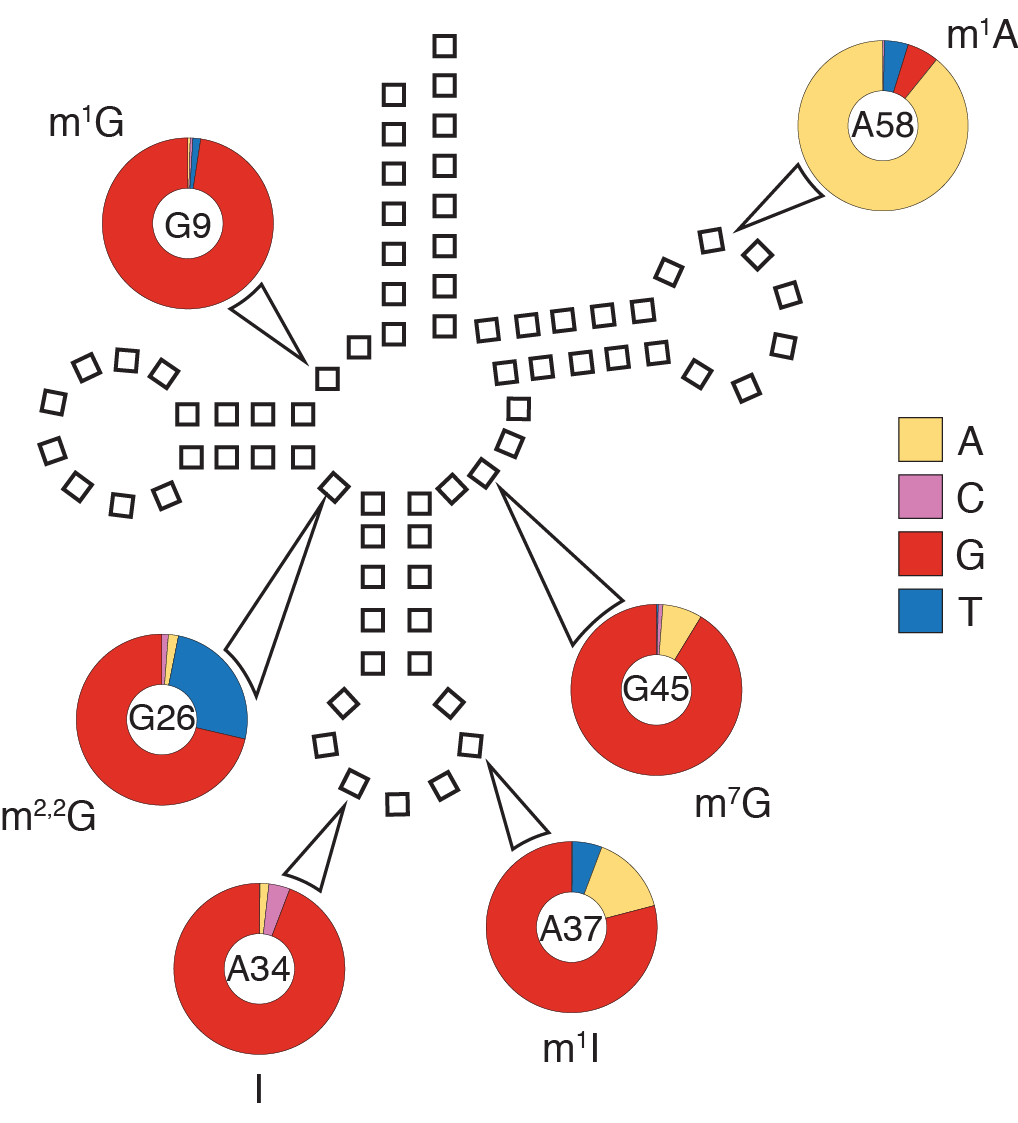
\includegraphics[scale=1]{paper7a.png}%
\caption[tRNA modifications detected by hydro-tRNAseq.]
{\textbf{tRNA modifications detected by hydro-tRNAseq.}
The positions that resulted in the most common mismatches over all tRNAs, along with the reference nucleotide and the most likely modification are indicated in the center of each ring. The relative frequency of each returned nucleoside is proportional to the corresponding color-coded area of the ring (m1G: 1-methylguanosine; m2,2G: N2,N2-dimethylguanosine; I: inosine; m1I: 1-methylinosine; m7G: 7-methylguanosine; m1A: 1-methyladenosine).}
\centering
\label{paper7a}%
\end{figure}

The temporal resolution of tRNA modifications by RNAseq has begun to be addressed recently  \cite{Torres:2015ed}, however at a single modification level (inosine 34), and by using libraries relative poor in tRNA reads (<1\% of total reads). I was appropriately poised to address this issue since my very deep sequencing set, in combination with my hierarchical annotation pipeline, offered the advantage of dissecting multiple modifications simultaneously. 

I focused on inosine editing events, since they represented the majority of modified nucleosides. By inspecting read alignments with error distance 1 to the reference pre-tRNA, I noticed A-to-G transition mismatches at position 34 in reads that retained the leader and trailer sequences of the precursor tRNA (\textbf{Fig. \ref{paper7b}, top}). 
This confirmed that A34 deamination takes place at the precursor level, and therefore is a nuclear modification, as it has been previously reported \cite{Torres:2015ed}. 

Next, I noticed that 1-methyl-inosine at position 37 also appears at the precursor stage. Of note the A37 modification became apparent prior to A34, as the majority of the error distance 1 reads contained a mismatch at A37. Reads with two mismatches contained both modifications (\textbf{Fig. \ref{paper7b}, bottom})

In many instances we observe specific and highly abundant mismatchsignatures in pre-tRNAs, which can possibly allow us to determine and monitor by RNA-seq the editing hierarchy of tRNAs and the order of function of their modifying enzymes. 

We observe editing in the D1 alignments. Those reads do not map at error distance 1, since we are following a hierarchical mapping, neither to they map back to the genome. This suggests that we can observe nucleotide editing at the precursor stage of tRNAs. 

%All in all, far from being a comprehensive analysis of tRNA editing and modifications, the work presented here outlines how a careful examination and analysis of deep hydro-tRNAseq datasets can yield valuable insights in the and type and temporal occurrence of such events. Such analysis is paramount to avoiding misassignment of sequencing reads when dealing with highly similar reference sequences. 

\begin{figure}[!ht]%
\centering
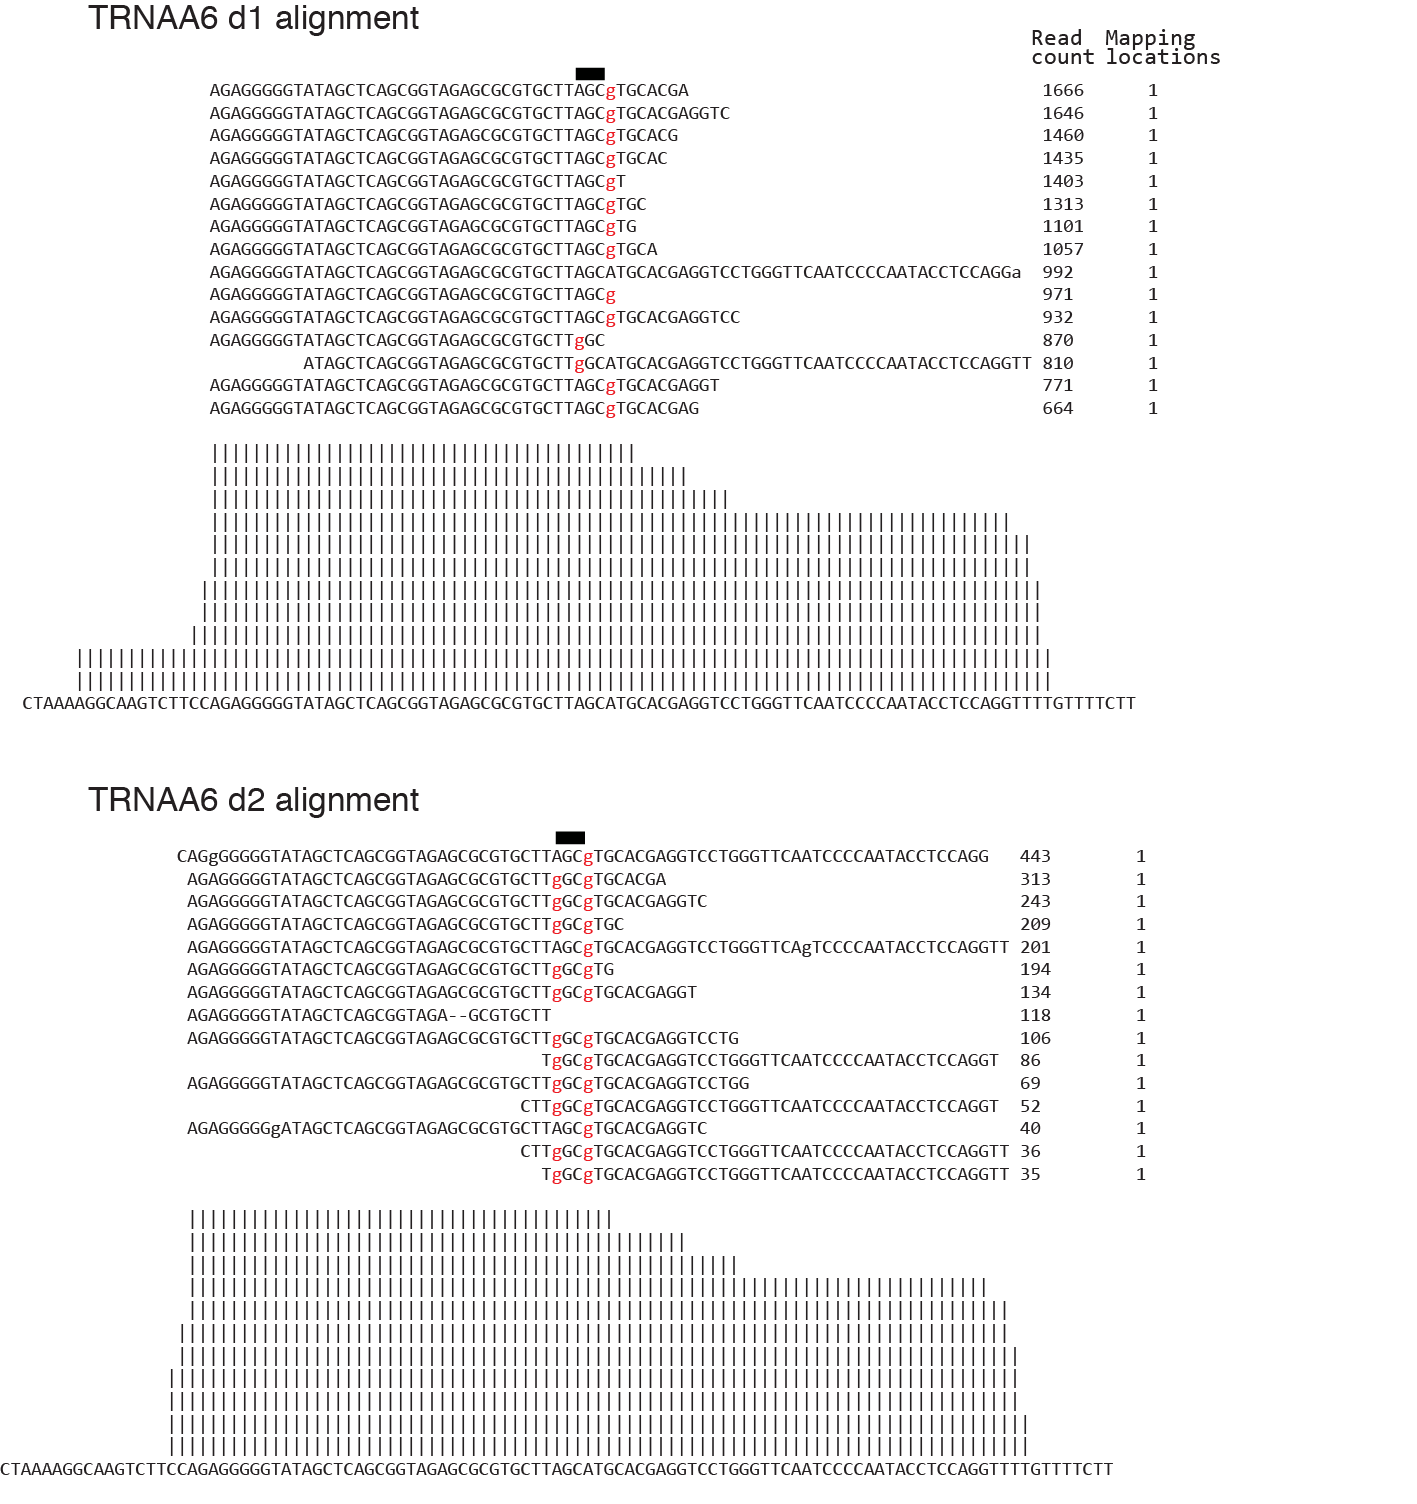
\includegraphics[width = 5in]{paper7b.png}%
\caption[Temporal resolution of tRNA modifications]
{\textbf{Temporal resolution of tRNA modifications.}
Read alignments for precursor TRNAA6 with one (top) and two mismatches (bottom). The position of the anticodon is marked by the black rectangle at the top of the alignments. Mismatches of the heavily modified adenosines in the anticodon loop are indicated by red lowercase letters. Read counts and mapping locations for each read are shown on the right side. Vertical bars represent binned, log4-transformed, and normalized read counts for each alignment.}
\centering
\label{paper7b}%
\end{figure}

\section{Annotation of intron-containing tRNA genes} \label{introns}

Intron-containing tRNAs represent a particularly interesting set of tRNA genes, as mutations in their evolutionarily conserved, yet distinct, processing machinery have emerged recently as causes of severe neurodevelopmental syndromes, such as pontocerebellar hypoplasia \cite{Cooper:2009da,Namavar:2011ew,Weitzer:2014bi} \hl{Budde 2008}. Therefore, there is documented need for a comprehensive annotation of human intron-containing tRNAs, which should be revisited as markers or disease-causing candidates in phenotypically similar conditions. 

\begin{figure}[!ht]%
\centering
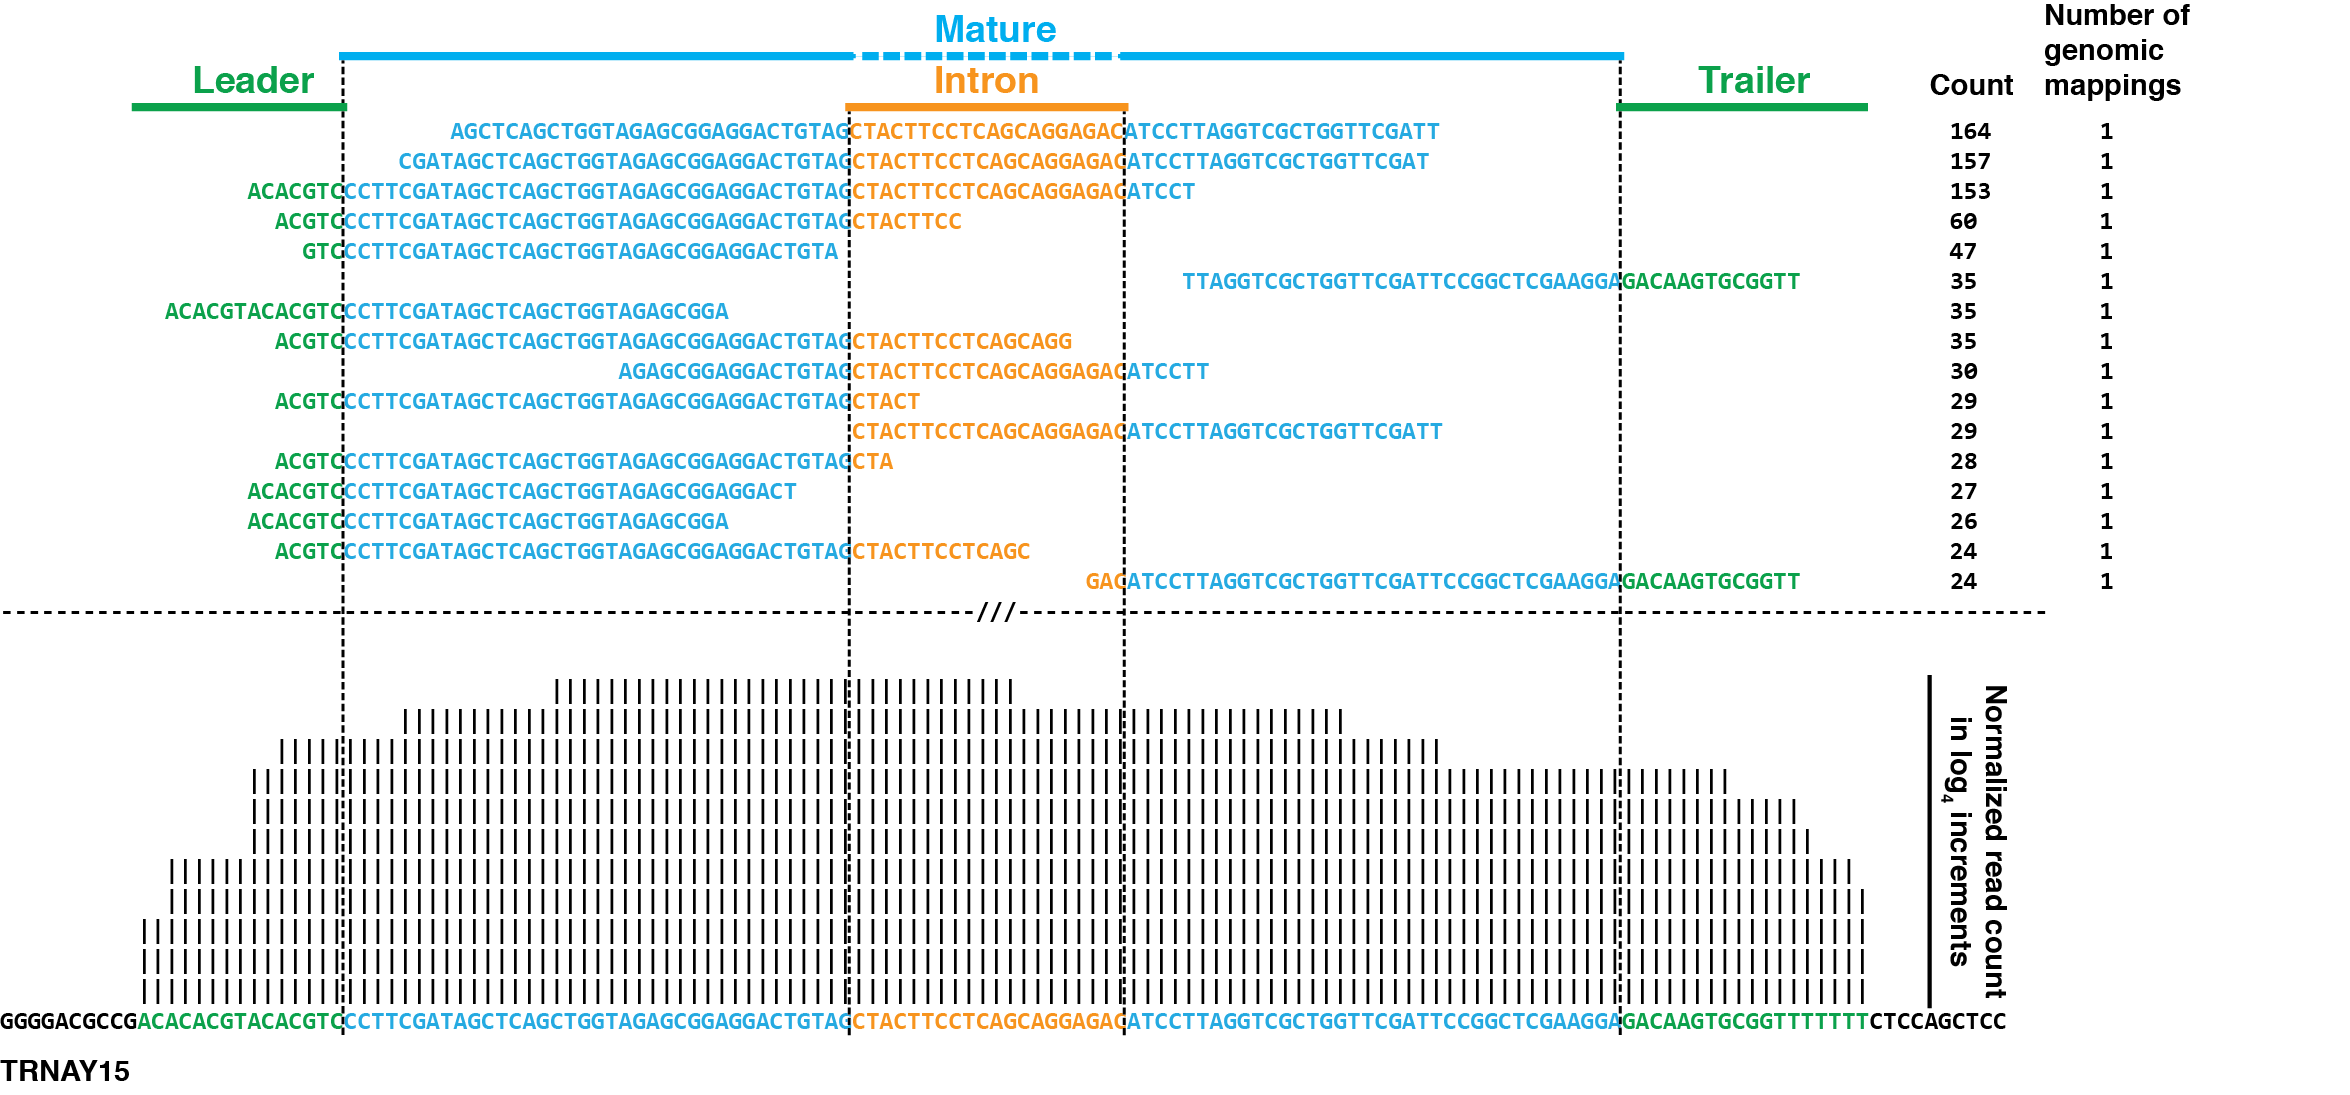
\includegraphics[width=\textwidth]{intron_trna.png}%
\caption[Intron-containing pre-tRNA alignment.]
{\textbf{Intron-containing pre-tRNA alignment.} An indicative alignment to pre-tRNA TRNAY15 is shown. Mature sequence is in blue, leaders and trailers in green, and intron sequences in orange. Precursor/mature tRNA borders are demarcated by vertical, dotted lines.}
\centering
\label{intron_trna}%
\end{figure}

I set out to document all intron-containg tRNAs. Read coverage across both exon/intron boundaries in the pre-tRNA alignments was a requirement for the validation of intron-containing tRNAs (e.g.\textbf{Fig. \ref{intron_trna}}).I confirmed 26 out of 32 predicted intron-containing tRNAs by hydro-tRNAseq (\textbf{Fig. \ref{paper5}A}).  Intriguingly, I could not confirm expression of any predicted \underline{intronless} tyrosine pre-tRNA gene. The same was true for isoleucine-TAT and leucine-CAA isoacceptors.Excluding any unknown biologically redundant mechanism, this suggests that the integrity of the tRNA splicing complex is essential for survival, at least in the studied cellular system. 

\newpage
\begin{figure}[!hb]%
\centering
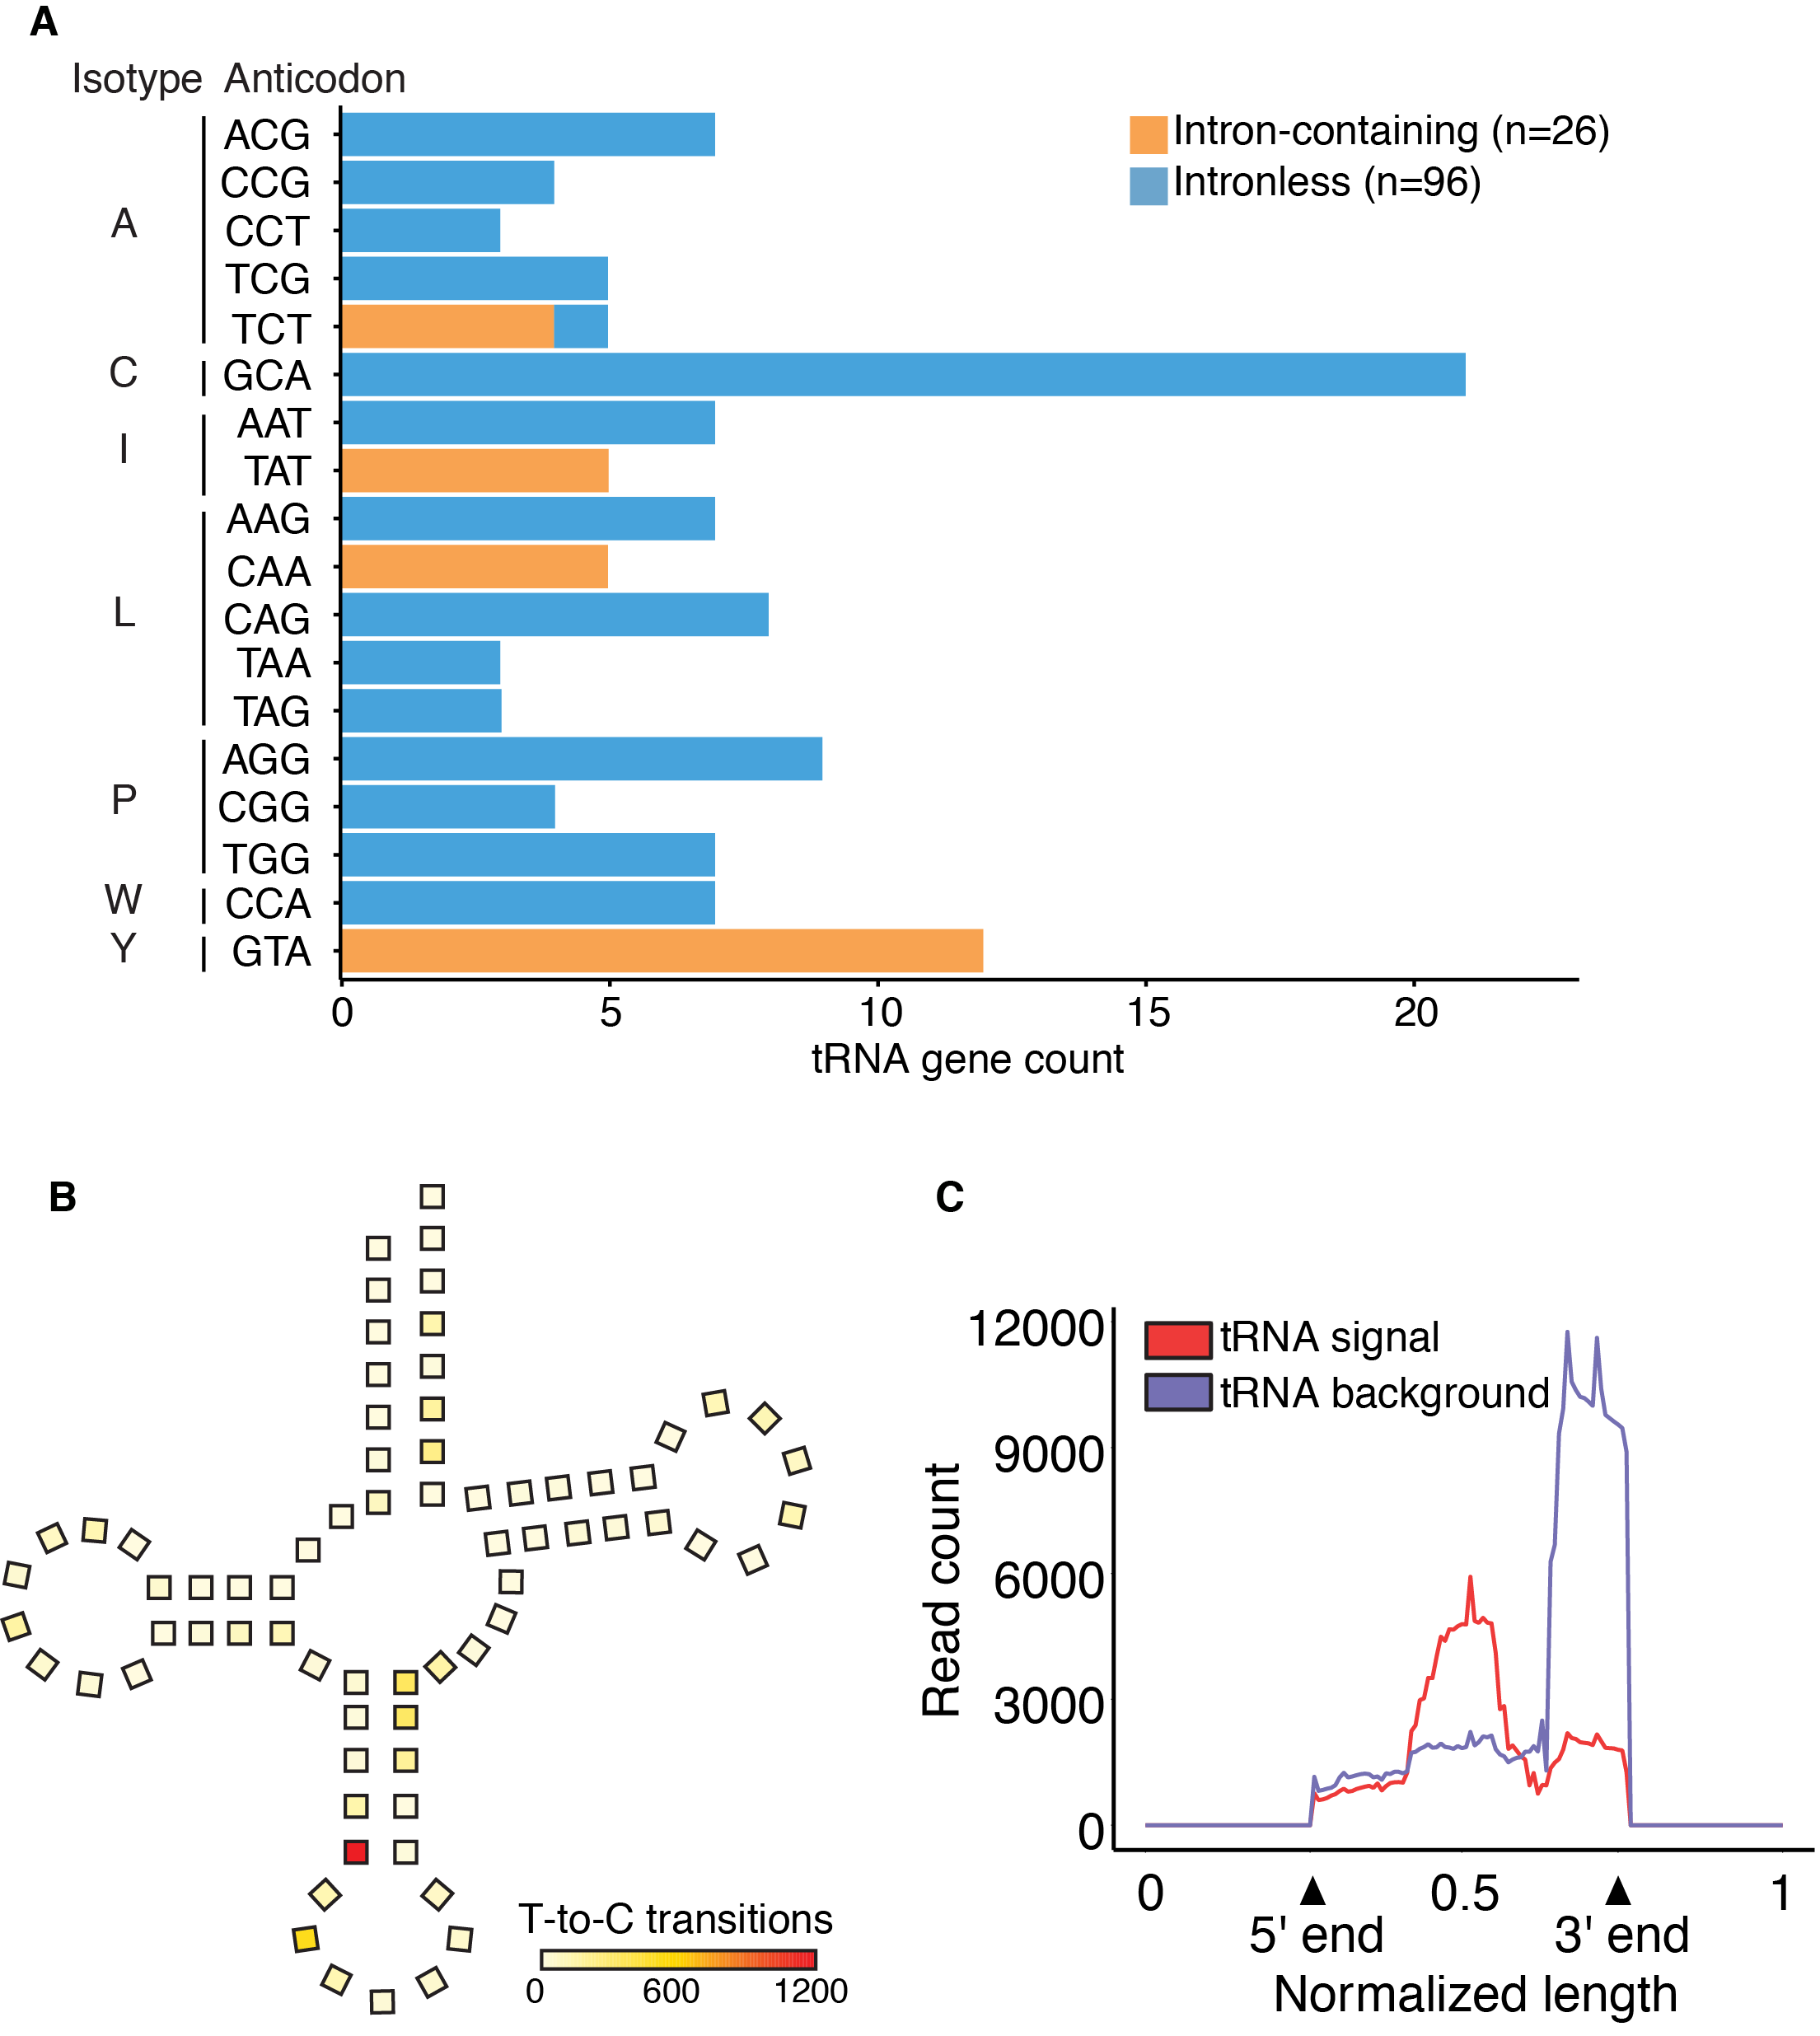
\includegraphics[width=\textwidth]{paper5.png}%
\caption[Annotation of intron-containing tRNA genes.]
{\textbf{Annotation of intron-containing tRNA genes.}
(A) Number of validated intron-containing (orange) and intronless (blue) tRNA genes for all tRNA isotypes with possible intron-containing tRNAs. (B), (C) Analysis of PAR-CLIP for the tRNA ligase, RTCB (previously published in (Baltz et al., 2012). Positional preference of crosslinking by metagene analysis of all crosslinking events (B) and all crosslinked reads (C) to mature tRNAs. The incidence of T-to-C transitions is indicated by color intensity in (B). PAR-CLIP signal (reads containing T-to-C), background (reads with no mismatches), normalized boundaries of the pre-tRNAs (labeled as 0, 1) and mature tRNAs (labeled as 5’ end, 3’ end) are shown in (C)
}
\centering
\label{paper5}%
\end{figure}

To further confirm my observations, I coupled hydro-tRNAseq results with previously published PAR-CLIP data on the human tRNA ligase, RTCB \cite{Baltz:2012bh}. Despite the shallow read depth of the dataset, I identified a crosslinking peak (RBP binding site) at the anticodon loop of all intron-containing tRNAs annotated by my approach (\textbf{Fig. \ref{paper5}B,C}. 

\section{Hydro-tRNAseq application in human disease}\label{clp1section}
These observations came at an opportune moment because of novel contributions of tRNA processing ongoing efforts to characterize the human disease involvement of \gls{CLP1}, a 5' RNA kinase involved in tRNA splicing \cite{Weitzer:2007hda}. Before my studies, it was shown that mouse models with CLP1 that lacked its catalytic activity develop severe neuromuscular defects accentuated by loss of motor neurons and muscular paralysis \cite{Hanada:2013bk}. 

Human exome capture and sequencing from individuals with ponotcerebellar hypoplasia identified a homozygous missense mutation in CLP1 (chr11:g.57,427,367 G > A [hg19], p.R140H) in five unrelated, but consanguineous families, resulting in an autosomal recessive pattern of inheritance (\textbf{Fig. \ref{pedigree}}). Biochemical studies showed that this autosomal mutation reduces the interaction affinity of CLP1 with the splicing complex \cite{Karaca:2014em}. 

\begin{figure}[!ht]%
\centering
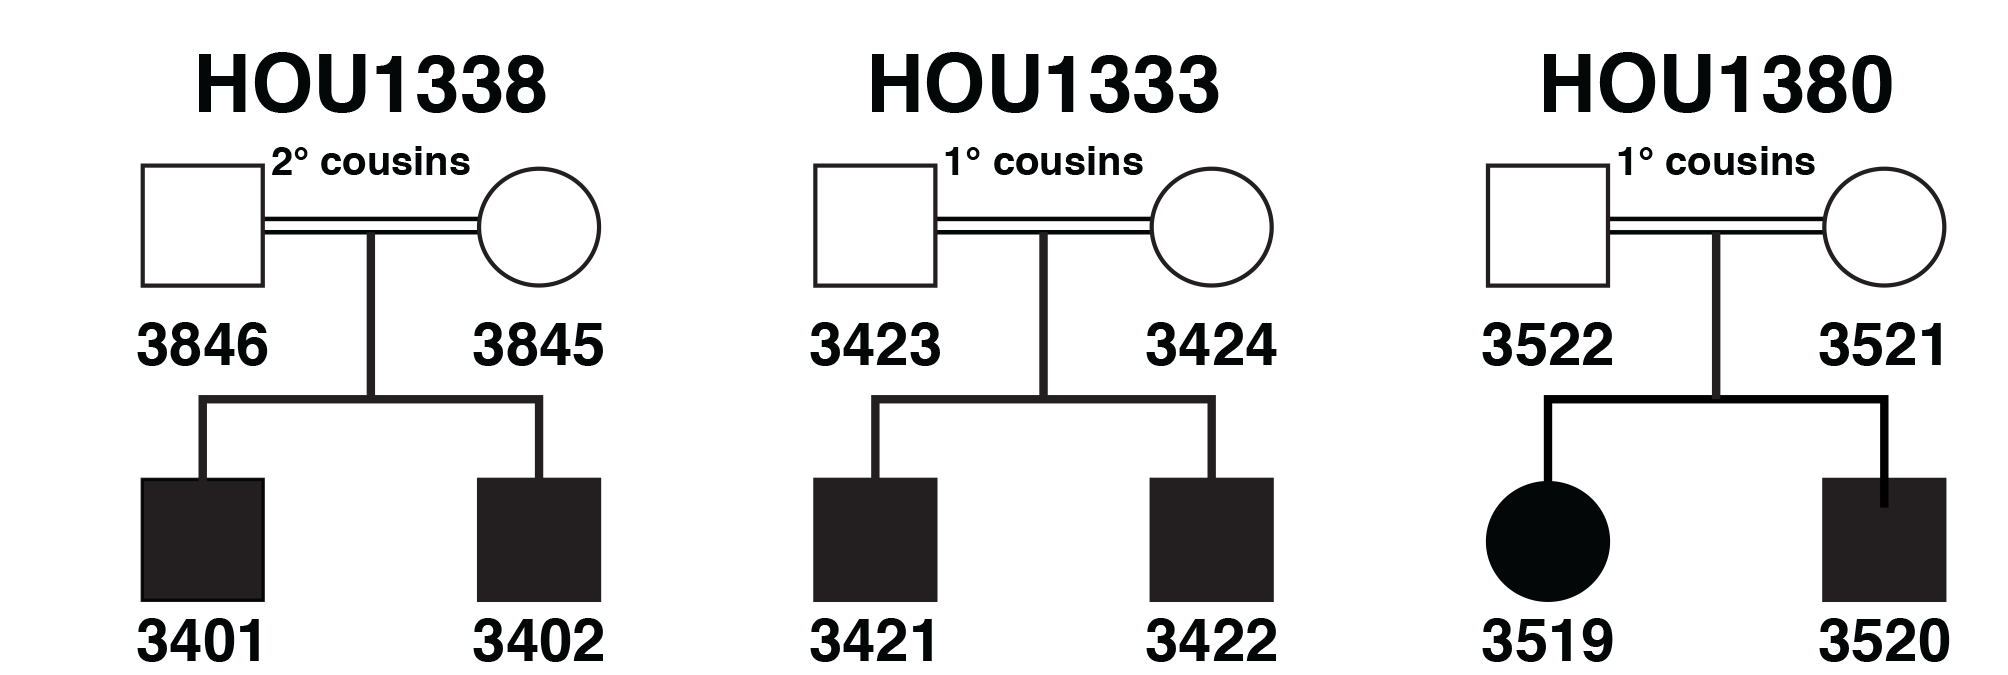
\includegraphics[width=\textwidth]{pedigree1.png}%
\caption[Pedigrees of families with CLP1-induced syndromes.]
{\textbf{Pedigrees of families with CLP1-induced syndromes.}
Pedigrees of three nuclear families with patients showing microcephaly, ponotcerebellar hypoplasia, dysmorphic facial features and severe neuromuscular abnormalities. CLP1 p.R140H follows autosomal recessive inheritance. Double lines indicate consanguineous marriages; squares and circles represent male and female subjects, respectively. Black-filled shapes indicate patients.}
\label{introntrna}
\end{figure}

However, it was not clear whether this had any molecular effect on tRNA processing. I applied Hydro-tRNAseq on RNA isolated from parental and patient fibroblasts. There was no significant difference in the steady-state levels of either mature (for example \textbf{Fig. \ref{clp1align}}, right part) or pre-tRNAs as reported by our bioinformatics pipeline. 

\begin{figure}[!ht]%
\centering
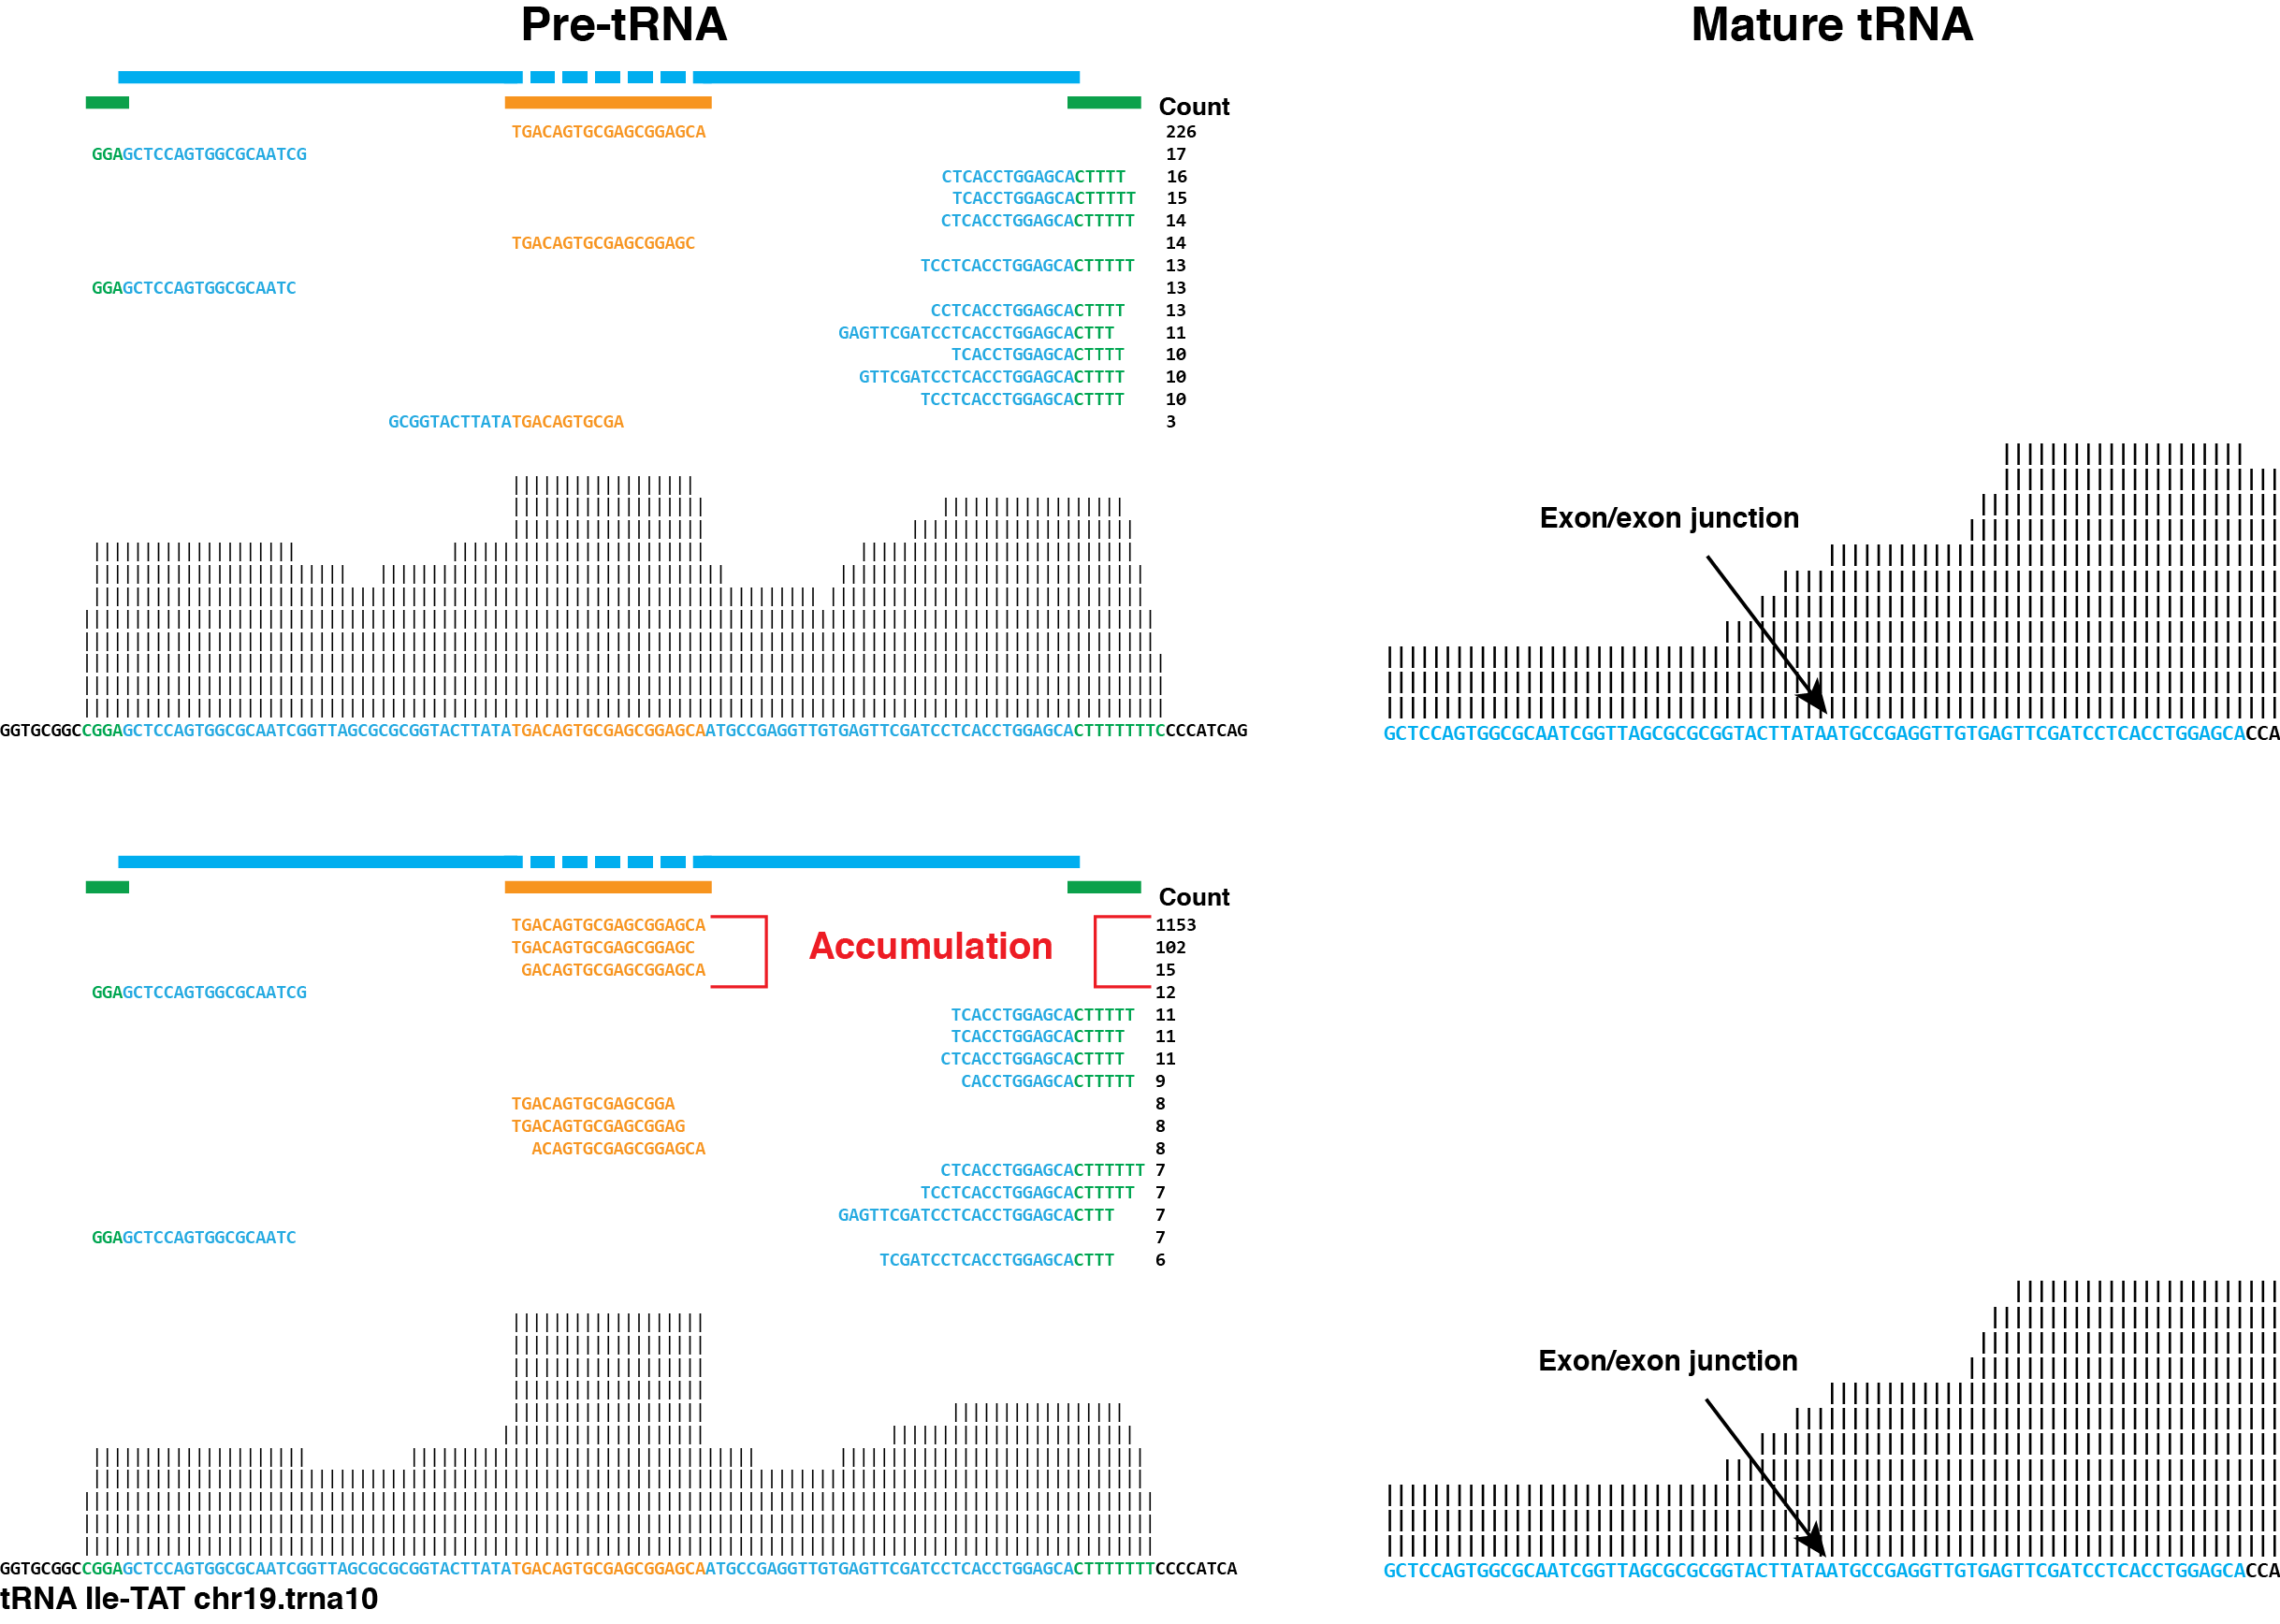
\includegraphics[width=\textwidth]{clp1align.png}%
\caption[Hydro-tRNAseq analysis of CLP1 patient fibroblasts.]{\textbf{Hydro-tRNAseq analysis of CLP1 patient fibroblasts.} 
Example of an isoleucine pre-tRNA (left part) and mature tRNA (right part) alignment for a matched parent (top) - patient (bottom) pair. Accumulate intronic reads are bracketed. The exon/exon junction is indicated in the mature tRNA alignments.}
\centering
\label{clp1align}%
\end{figure}

Interestingly, however, when I manually inspected I detected reproducibly an accumulation of intronic sequences for specific pre-tRNAs (\textbf{Fig. \ref{clp1align}}, left part) in patient samples. The same pattern was observed in two more pre-tRNAs, all of which showed >4-fold accumlation of intronic sequences (\textbf{Fig. \ref{clp1bars2}}).

\begin{figure}[!ht]%
\centering
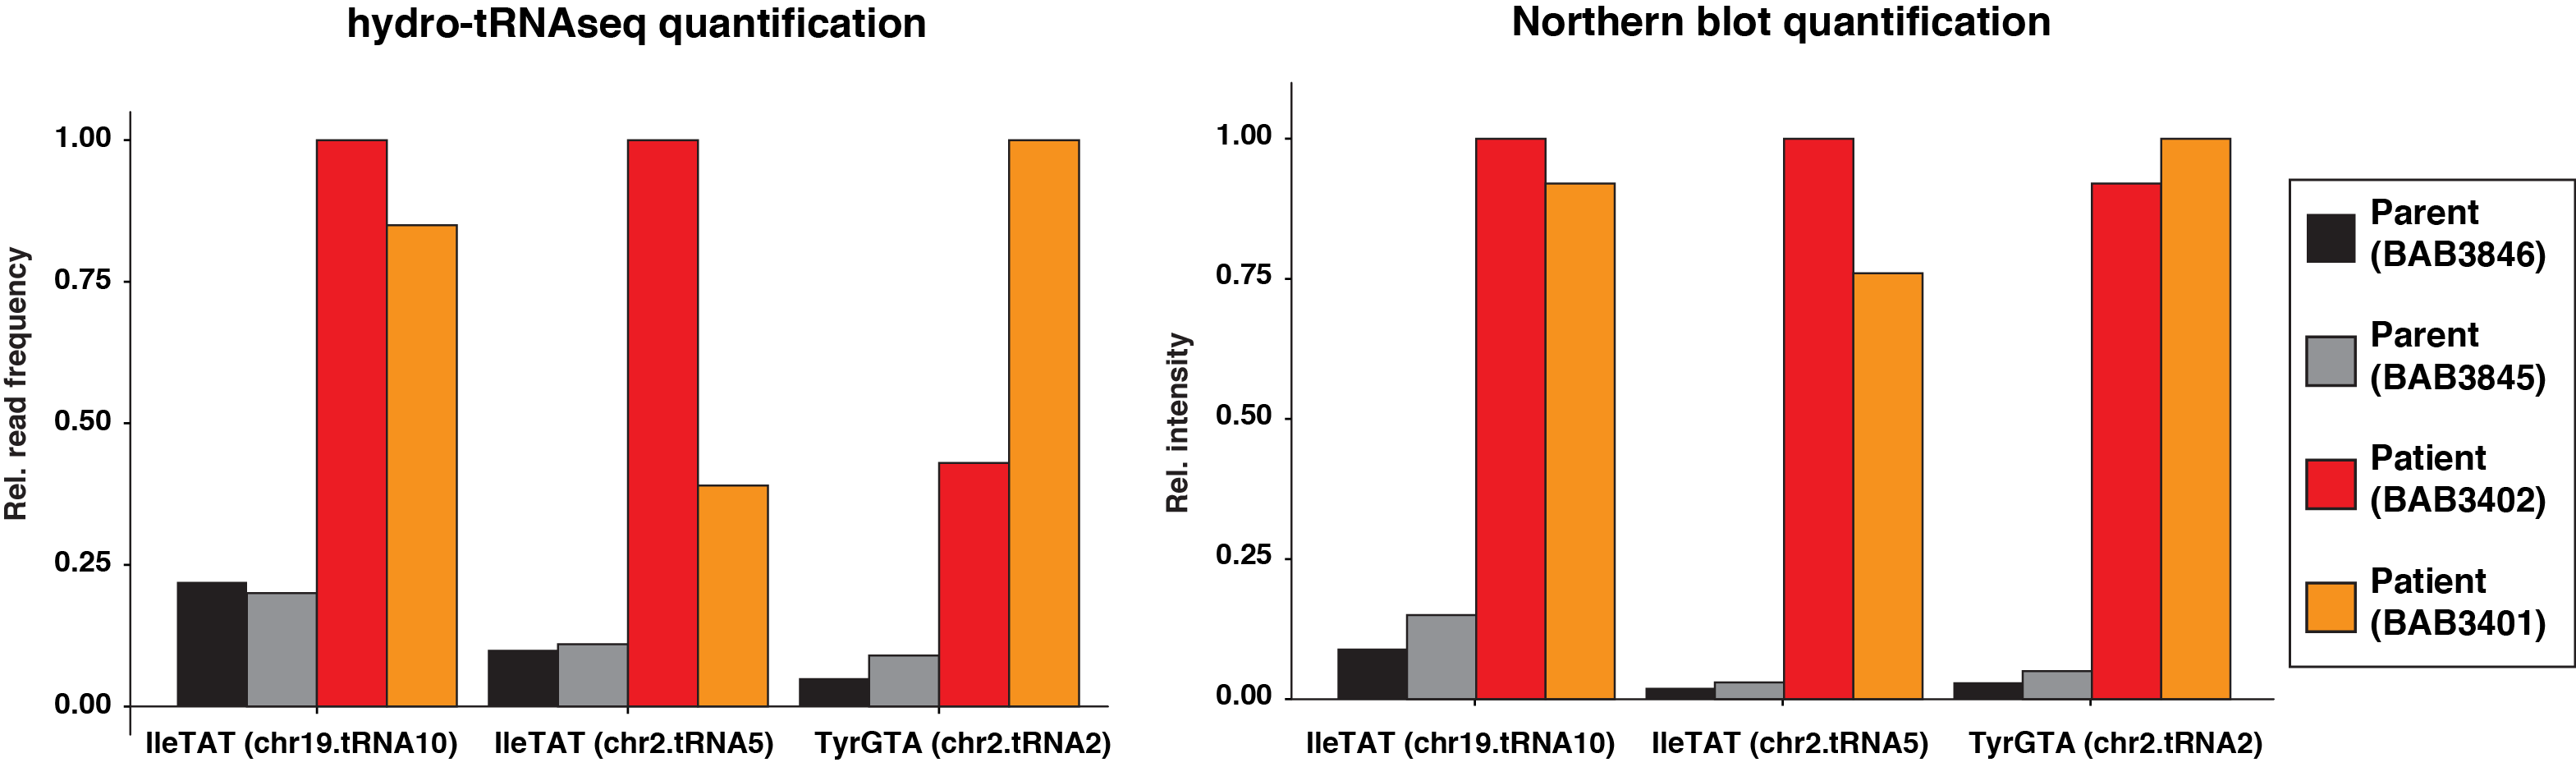
\includegraphics[width=\textwidth]{clp1bars2.png}%
\caption[CLP1 mutation leads to intronic read accumulation.]
{\textbf{CLP1 mutation leads to intronic read accumulation.}
Quantification of intronic reads for three different pre-tRNAs for parents (black and grey bars) and patients (red and orange bars). Hydro-tRNAseq data shown on the left, and northern blot data on the right.}
\centering
\label{clp1bars2}%
\end{figure}

These results were confirmed independently by our collaborators (Stefan Weitzer, Javier Martinez, IMBA) who carried out northern blot analysis on the same RNA samples. Consistent with my results, they failed to detect significant differences in steady-state mature or pre-tRNA levels between parents and patients (\textbf{Fig. \ref{nb}}, top-most pannels), but detected an accumulation of the salient tRNA introns of my analysis (\textbf{Fig. \ref{nb}}, middle pannels). Densitometric analysis of the northern blots also confirmed the trend and range of intron accumulatino across the studied samples (\textbf{Fig. \ref{clp1bars2}}), proving that th two techniques are in good agreement. 

\begin{figure}[!ht]%
\centering
\includegraphics[width=\textwidth]{nb.png}%
\caption[Northern blot analyses of RNA from parental and patient fibroblasts.]
{\textbf{Northern blot analyses of RNA from parental and patient fibroblasts.}
A probe complementary to the 50 exon of isoleucine-TAT and tyrosine-GTA tRNAs was used to detect mature and pre-tRNA species (top panels). Probes specifically directed against intron sequences were used to detect pre-tRNAs and tRNA introns of two isoleucine-TAT and one tyrosine-GTA tRNAs (middle panels). U6 snRNA served as loading control (bottom panels). Asterisks denote truncated pre-tRNA species.}
\centering
\label{nb}%
\end{figure}

\subsection{Plausible pathomechanisms of CLP1 mutations}\label{clp1_evolution}
	Thus, our Northern analysis and deep sequencing data indicate that the CLP1 R140H mutation in fibroblasts influences processing of pre-tRNAs, resulting in the accumulation of tRNA introns, whereas pre- and mature tRNA levels remain largely unaffected. Nevertheless, at this point the biological mechanisms responsible for the pathogenicity of CLP1 mutations are not clear.

\begin{figure}[!ht]%
\centering
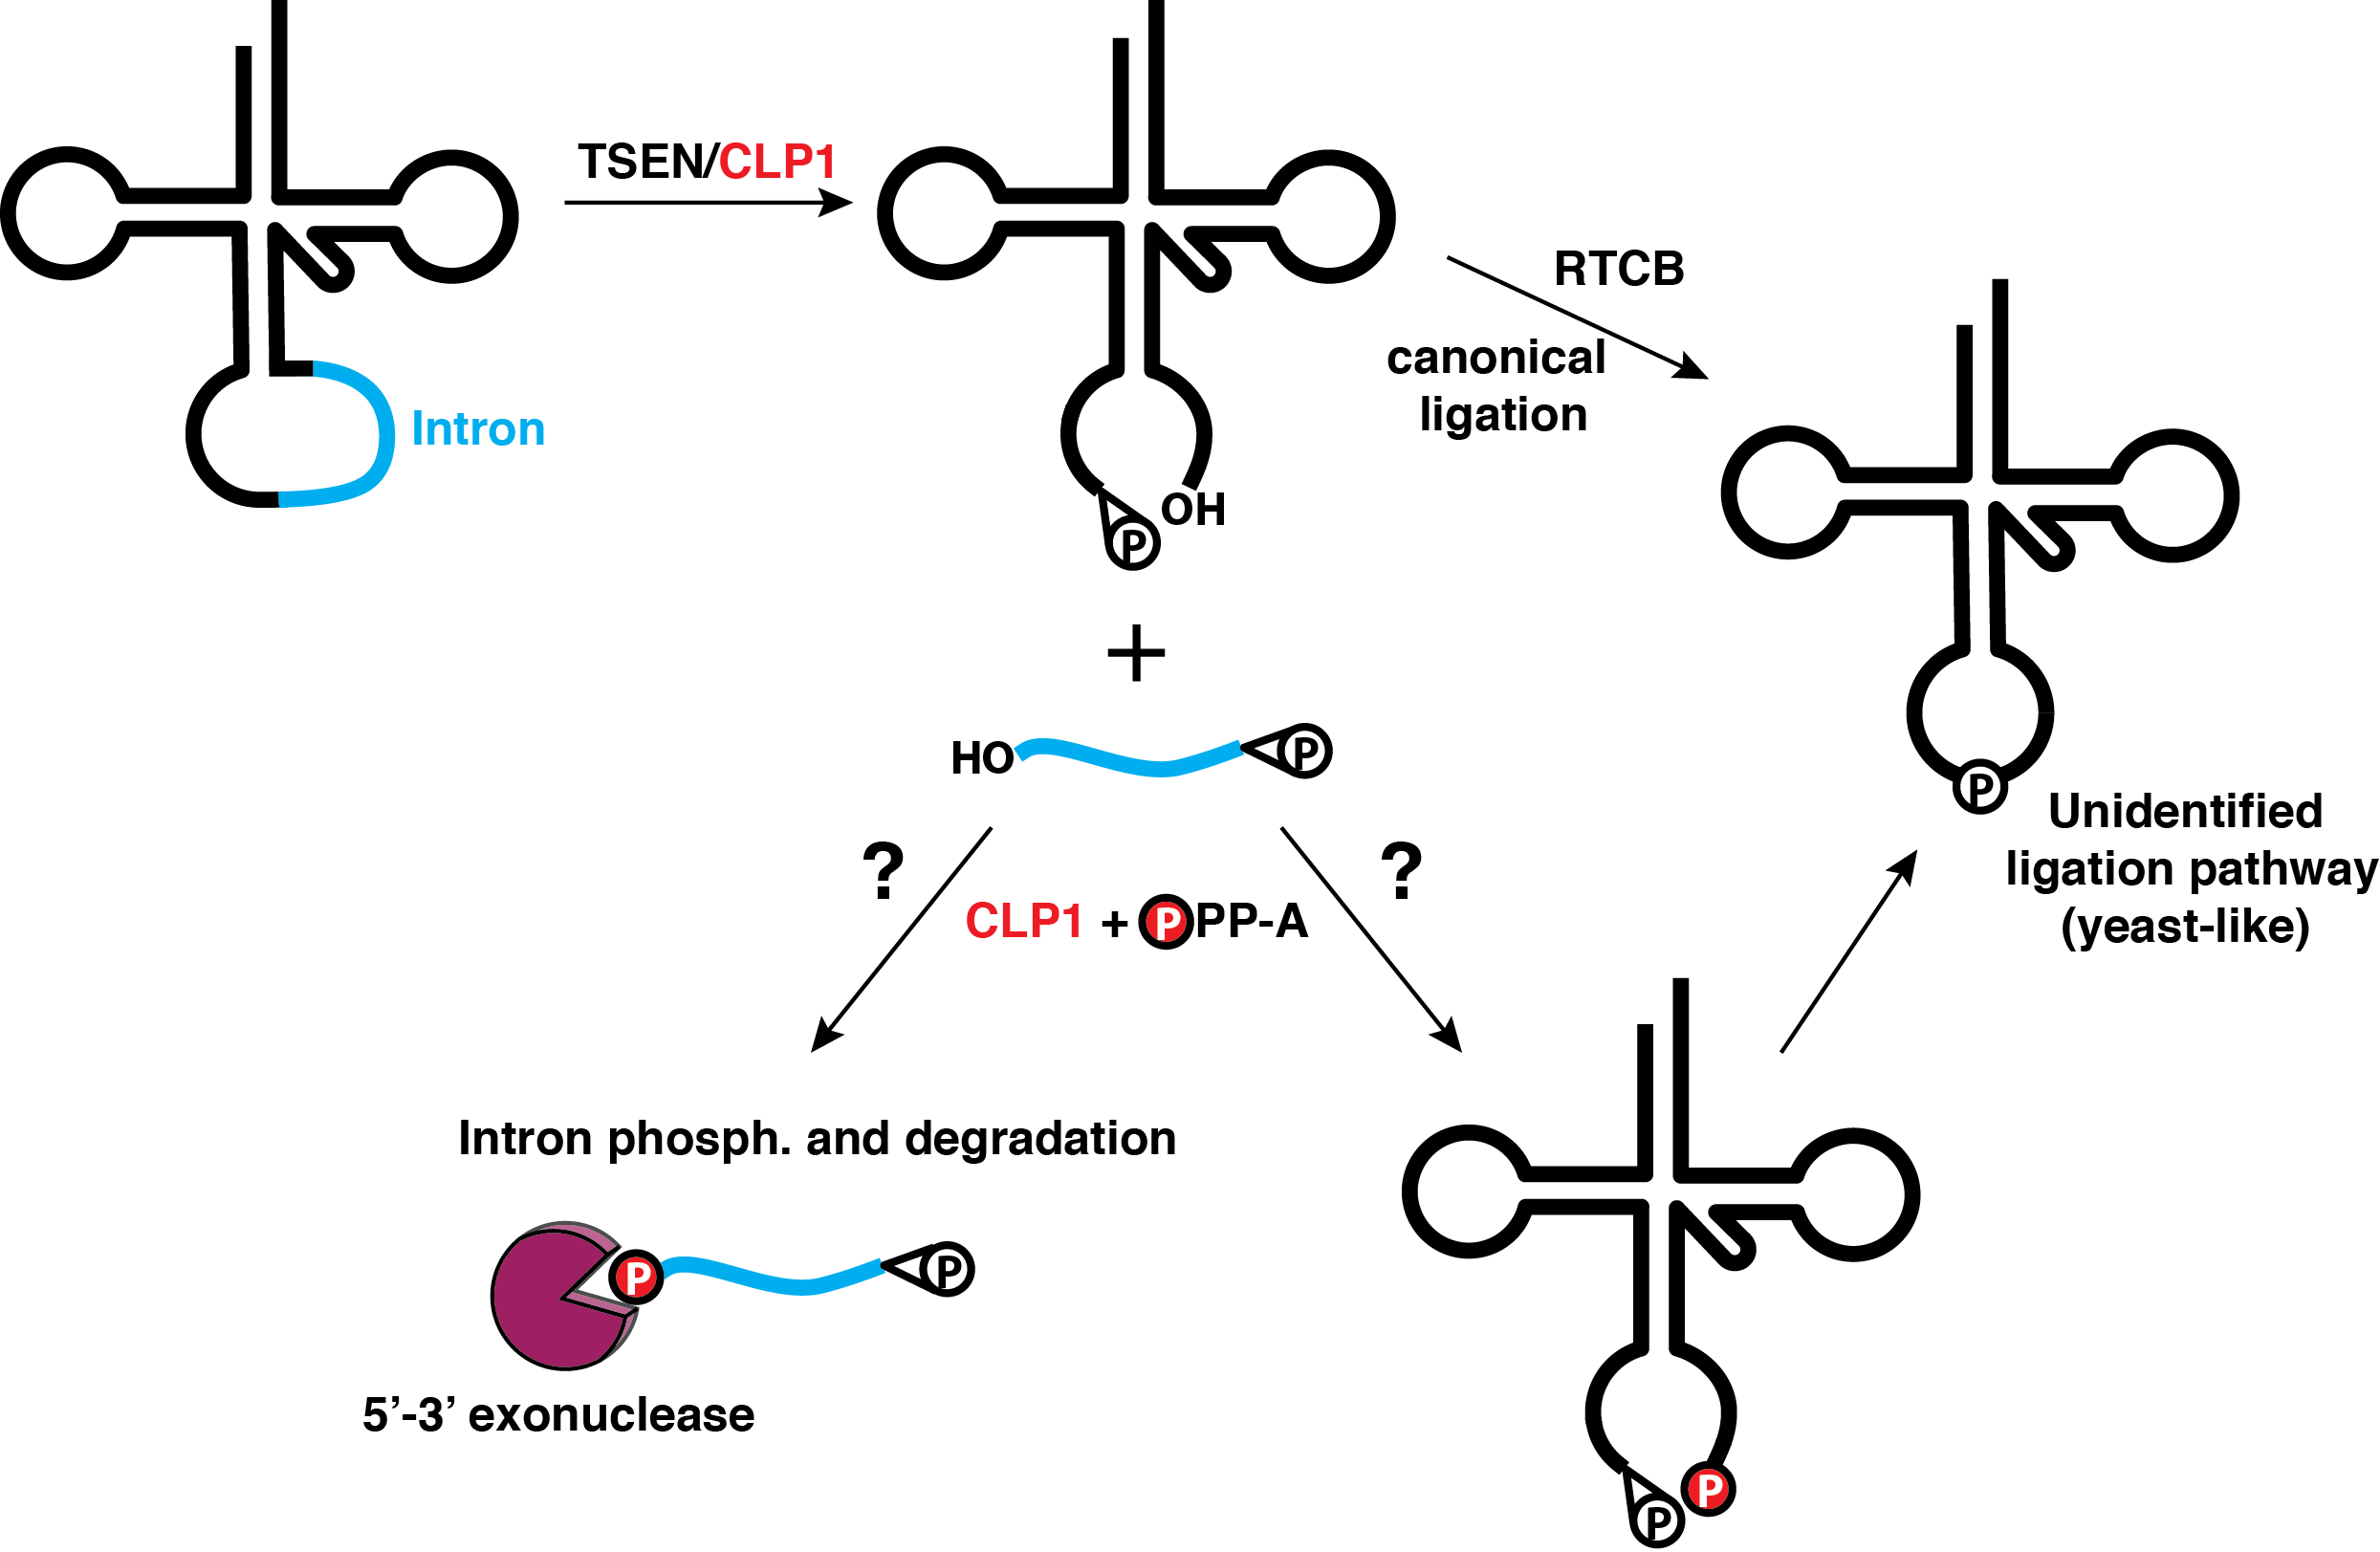
\includegraphics[width=\textwidth]{splicing2_v2.png}%
\caption[Model of CLP1 involvement in tRNA splicing.]
{\textbf{Model of CLP1 involvement in tRNA splicing.}
CLP1 associates with the TSEN complex, which endonucleolytically removes tRNA introns (labeled in blue). The cleavage results in a 3' cyclic phosphate and 5' OH on the 5' and 3' exons, respectively, which are ligated by RTCB (canonical ligation). CLP1 can also phosphorylate the 3' exon which could then be ligated to the 5' half by an unknown ligase. CLP1 could also phosphorylate the removed intron facilitating its removal by an exonuclease.}
\centering
\label{splicing}%
\end{figure}

During intron removal, cleavage by \gls{TSEN} leaves a 3' cyclic phosphate on the 5' tRNA exon and a 5' OH on the 3' exon (\textbf{Fig. \ref{splicing}}). These moieties are substrates of the tRNA ligase (RTCB), which carries out the ligation of the two tRNA halves. CLP1 is capable of phosphorylating the 5' end of the 3' exon, possibly allowing the ligation of the two halves by a yet unknown ligase \cite{Weitzer:2007hda}, which would be reminiscent of the tRNA splicing pathway in yeast \cite{Weitzer:2014bi}. 

Alternatively, CLP1 could be phosphorylating the removed intron, which harbors a 5' OH immediately after cleavage. The "healing" of the 5' end of the linear intron is a requirement for its degradation, at least in yeast, by the 5'-3' exonuclease Xrn1 \cite{Wu:2014fb}.
Altogether, taking into account both the documented and hypothesized functions of CLP1, one could come up with the following testable hypothesis regarding the plausible pathomechanisms of CLP1 mutations:
	
\begin{itemize}
\item tRNA splicing and mature tRNA levels are reduced in metabolically in sensitive tissues (e.g. neurons), while they are unaffected in fibroblasts.
\item tRNA intron accumulation leads to innate immunity activation.
\item tRNA splicing proteins have pleiotropic, and possibly tRNA-unrelated effects (e.g. participation in mRNA polyadenylation \cite{Paushkin:2004wl, Weitzer:2014bi})
\end{itemize}

%\section{tRNA enzyme screen}
%With respect to more functional aspects of tRNA biology, I focused on the results from knockdowns from a series of tRNA modifying and processing enzymes. Surprisingly, even though I targeted key components of the tRNA biogenesis and processing pathway, I could not observe major defects in tRNA processing or abundance patterns with the exception of the tRNA ligase (RTCB) that led to a very modest accumulation of 5’ end tRNA halves. This suggested either that the residual enzymatic activity after knockdown is sufficient for proper tRNA processing or that there is unknown redundancy in several steps of tRNA biogenesis. 

%This publication steered interest in the connection of tRNA and disease, a link that was previously not well examined. To further showcase the utility and usefulness of my method in this field I decided to use it in a proof of principle example. I have carried out an siRNA-mediated gene silencing screen targeting a series of tRNA processing and modifying enzymes (i.e. the CCA terminal transferase, the tRNA methyltransferase TRMT10A, the tRNA splicing ligase HSPC117, a member of the RNase P complex, and also TRANSLIN, a putatively novel tRNA processing enzyme – see aim 2). In the cases where a reliable antibody was available, the knockdowns were validated by western blot analysis. In all other cases, knockdowns are currently being validated by mRNAseq. RNA from the validated knockdowns will be subjected to tRNAseq, with the expectation to identify tRNA processing defects that prior to our method would have been overlooked. In addition, I have performed tRNAseq from spinal cord-derived fibroblasts of knockout mice for the tRNA ligase. There I was already able to show tRNA processing is affected characterized by an accumulation of unspliced tRNA halves. 

\section{Comparison with other methods}

Recently tRNA sequencing methods have been developed that employ dealkylating enzymes and/or highly thermostable reverse transcriptase to overcome respectively the hurdles of modifications and stable structures that impede tRNA sequencing \cite{Cozen:2015ds, Zheng:2015dw}. However, they both have specific limitations that I tried to address. I size-selected at a higher size window to avoid contamination by tRNA-derived fragments (as compared to \cite{Cozen:2015ds}). Also, I used two sequential adapter ligation methods to make sure that only full-length fragments were sequenced and the sequencing reads were not results of blocks during RT (as compared to \cite{Zheng:2015dw}), which allowed me to differentiate RT stops from fragment ends. Additionally, I did not bias our sequencing protocol towards mature tRNAs, but instead captured more precursors by both hydro-tRNAseq and more importantly PAR-CLIP methods, which enabled a deeper pre-tRNA curation. Importantly, despite the reportedly high processivity conferred by dealkylating methyl modifications, in the previous studies only a small fraction of reads mapped at a given transcript were full-length reads (<1\% of all reads), with a marginal increase compared to untreated controls (\textbf{Fig. \ref{supp6}}). 

\begin{figure}[!ht]%
\centering
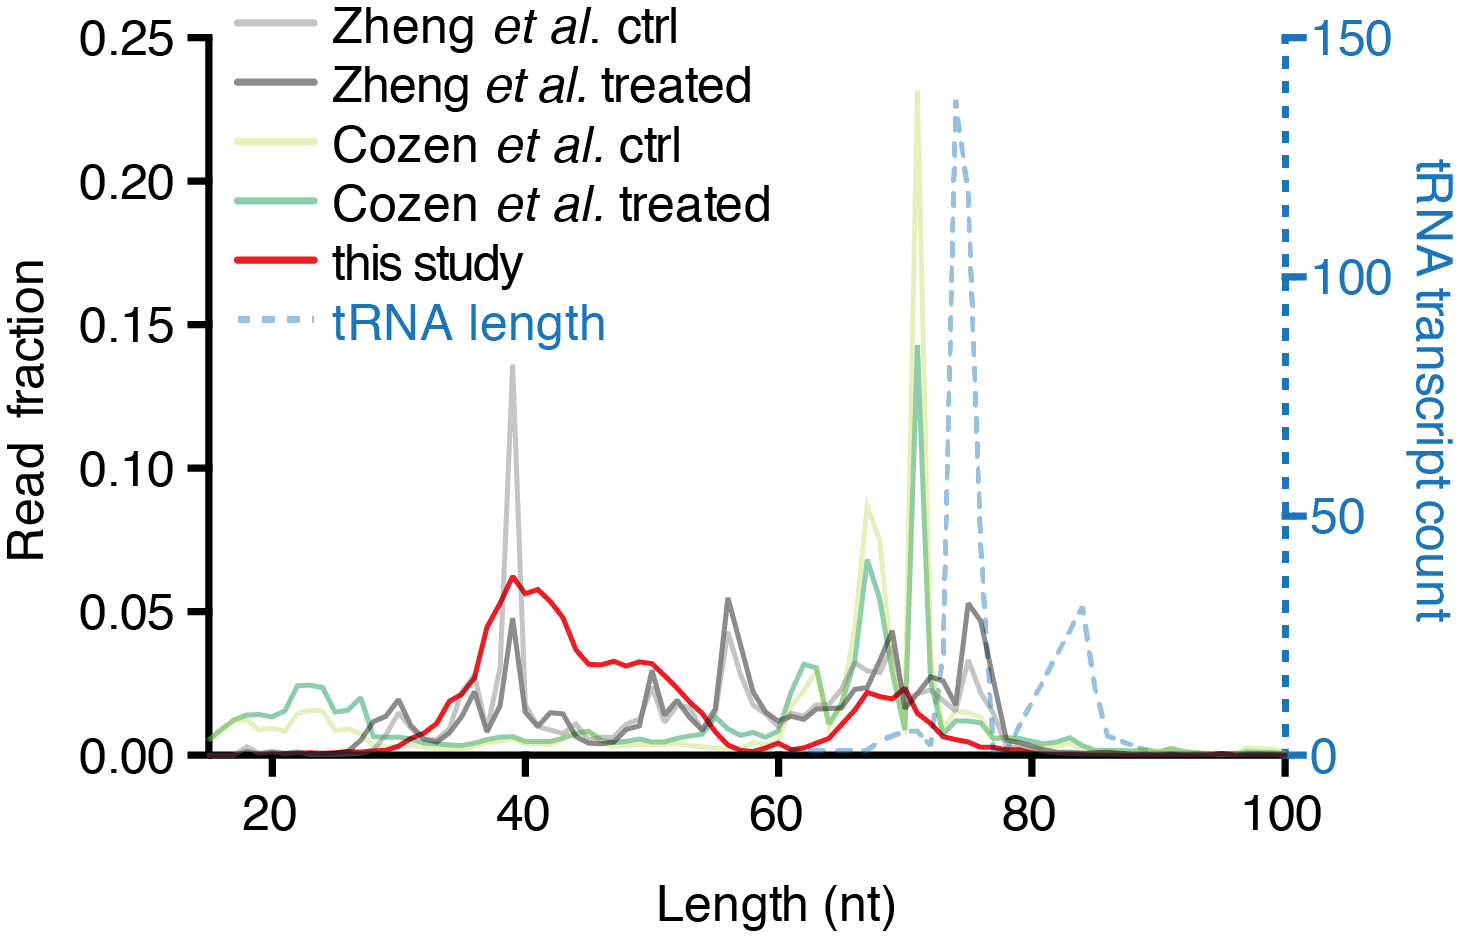
\includegraphics{supp6.png}%
\caption[Read length distribution for hydro-tRNAseq and dealkylating sequencing methods.]
{\textbf{Read length distribution for hydro-tRNAseq and dealkylating sequencing methods.}
Histogram representing the fraction of normalized mature tRNA transcript length with ungapped and overlapping read evidence in hydro-tRNAseq and tRNA sequencing methods employing dealkylation steps (control and subjected to treatment). The mean fraction is indicated next to each method.}
\centering
\label{supp6}%
\end{figure}

In contrast, hydro-tRNAseq yielded a higher cumulative fraction of mature tRNAs with read evidence across their whole length with a mean read coverage of 0.99 of the full length (compared to 0.95 and 0.87 in previous studies; \textbf{Fig. \ref{supp7}}). Also, SSB PAR-CLIP was more sensitive in identifying tRNA genes, detecting 349 genes as compared to ~159 and ~212 in the other methods.

\begin{figure}[!ht]%
\centering
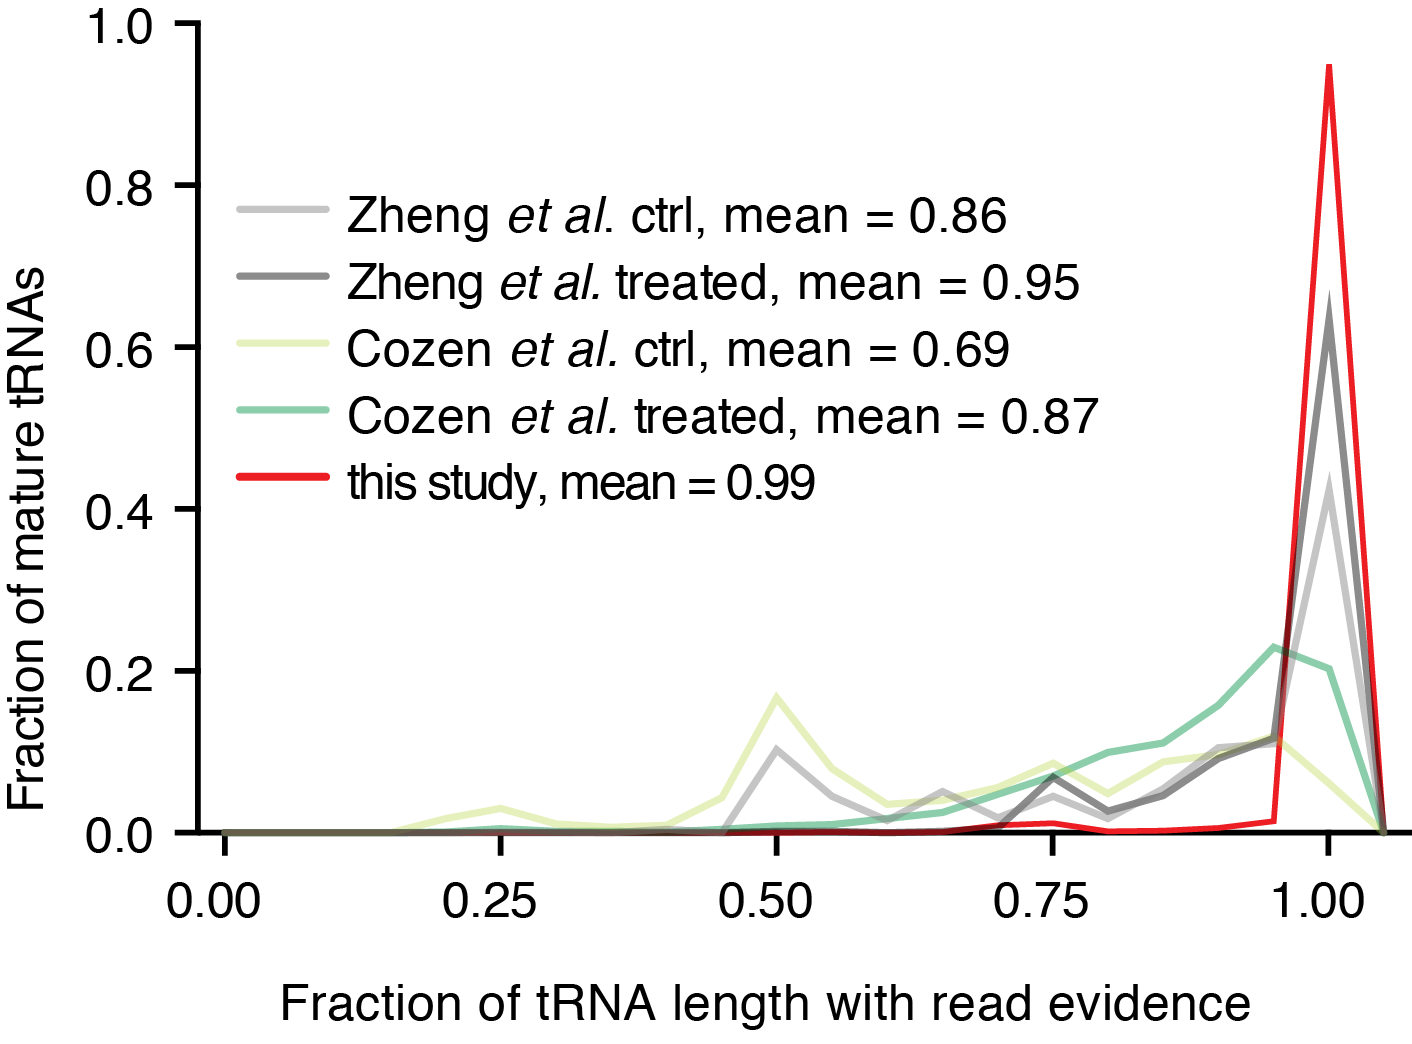
\includegraphics{supp7.png}%
\caption[Mature tRNA read coverage by hydro-tRNAseq and dealkylating sequencing methods.]
{\textbf{Mature tRNA read coverage by hydro-tRNAseq and dealkylating sequencing methods.}
The fraction of reads with a given length is indicated for hydro-tRNAseq, as well as untreated and treated samples from dealkylating methods. The distribution of tRNA lengths is shown in dotted blue lines on the right y-axis for comparison.
}
\centering
\label{supp7}%
\end{figure}


\section{Discussion}
I have combined two complementary transcriptome-wide approaches to provide experimentally validated annotation for mature and pre-tRNA transcripts and their respective genes, in addition to furnishing an accurate quantification of tRNA abundance in human cells.

First, I developed hydro-tRNAseq, a fragmentation-based protocol for overcoming hurdles of tRNA sequencing, and obtained deep sequencing sets that enabled the annotation of tRNA genes and derivation of mature tRNA reference sequences for accurately assigning sequence reads to the otherwise edited and nucleotide-modified original tRNA pool. Alkaline hydrolysis of the tRNA-containing pool relieved thermodynamically stable structural constraints that impair ligation steps in the cDNA library preparations, reduced the number of modified nucleosides per sequenced fragment, resulting in high read-through in the RT step, and release of the 3’ hydroxyl group of the otherwise aminoacylated tRNA 3’ end. 

Then, I took advantage of the pre-tRNA binding properties of SSB protein, which coordinates posttranscriptional processing and maturation of tRNAs \cite{Maraia:2010kx}, to enrich for tRNA precursors and allow for a comprehensive curation of pre-tRNA transcripts and annotation of tRNA genes. Of note, since SSB interacts with pre-tRNAs and other small nuclear RNA's U-rich 3’ ends in all organisms examined so far \cite{Maraia:2006in,Teplova:2006dv}, this approach can be adapted towards tRNA annotation in other species.

My data suggest that, at least in my experimental system, the tRNA gene space is considerably more contracted than it has been previously predicted by bioinformatics, evidenced by the fact that almost half of the predicted tRNA loci were transcriptionally silent, presumably representing retrointegrated tRNA pseudogenes or epigenetically silenced regions. It would be interesting to examine whether such an observation holds for various cell types and at different stages of development or disease, in order to confirm the differential expression and regulation of tRNA gene expression that has been reported before \cite{Gingold:2014iz,Goodarzi:2016gd}. 

Furthermore, my approach allowed the elucidation of relevant issues regarding POLR3 transcription such as the length of pre-tRNA leaders and trailers, the length of oligoU required for recognition by SSB, both of which have shown species specificity \cite{Arimbasseri:2015jg}. I detected that 4 sequential Us act as the transcription termination signal for POLR3, confirming similar predictions based on genomic sequences that suggested a requirement for 4 Us for efficient termination in vertebrates \cite{Arimbasseri:2013by,Iben:2012cy}, as well as structural data documenting the capacity of SSB to accommodate 4 Us in its binding site \cite{Stefano:1984wp,Teplova:2006dv}. At the same time, the length distribution of the oligoU tract identified in our experiments reflects the heterogeneity of termination signal lengths that has been noted as an intrinsic property of polymerase III \textit{in vitro} \cite{Arimbasseri:2015jg}.

I could also confirm a second binding site of SSB in the 5’ half of the mature tRNA sequence, in support of previous observations proposing the presence of additional pre-tRNA binding sites besides the 3’ tail \cite{Bayfield:2009cx,Stefano:1984wp}. It has been previously noted that the binding mode of SSB to tRNA is more complex than the recognition alone of the 3’ tails, and that one of the RNA recognition motifs present in SSB, RRM1, could bind elsewhere in the tRNA. This stems from two observations:
\begin{enumerate}[i)]
\item SSB has a higher affinity for precursor over mature tRNAs, 
\item structural data show that RRM1 is unoccupied when SSB is bound to UUU-3’-OH substrate.
\end{enumerate}
My data seem to validate this observation, and could shed light into new modes of SSB-mediated processing of pre-tRNAs into either mature tRNAs or other kinds of ncRNAs \cite{Hasler:2016ce}. 

Moreover, I were able to carry out a careful overview and tRNA modifications that result in characteristic mismatch signatures. I introduced all possible combinations of all “mutated” nucleotides at the most prominently modified positions in every tRNA in order to collect as many reads that could be having RT misincorporations at the modified positions. This created a large number of similar tRNA sequences, and therefore I allowed for extensive multimapping, but split the read counts in order to avoid artificial read count inflation. By making use of our hierarchical annotation pipeline, I was able to dissect the temporal order of inosine modifications at the tRNA anticodon, confirming that A34 deamination occurs in the nucleus prior to the nucleolytic processing of the pre-tRNA, and establishing that the same holds true for A37 modifications, which in fact precede A34 deamination. 

Accounting for modification signatures was also important for the reason that CLIP-seq, and especially PAR-CLIP, depends on apparent mismatches (in the case of PAR-CLIP, T-to-C conversions) for the identification of RBP binding sites on target RNAs. Since I used PAR-CLIP of SSB for the annotation of pre-tRNAs and tRNA genes, I first examined uridine modifications that result in T-to-C conversions. Only a small minority of modification signatures were T-to-C transitions, suggesting that it is highly unlikely that our PAR-CLIP data were artificially inflated. 

Then, I applied my protocols towards the elucidation of mechanisms of human disease, in a multi-collaborative effort to characterize a novel, severe neurodevelopmental syndrome caused by mutations in the tRNA kinase CLP1 \cite{Karaca:2014em}. By applying the hydro-tRNAseq protocol and analysis pipeline, I identified the accumulation of intronic sequences in the patient samples, a finding which was confirmed independently by Northern blot analysis. This constituted a demonstrative proof-of-principle that tailored-RNAseq protocols can be of considerable value in the context of diagnostics. 

\section{Summary}
In summary I have shown that: 

Collectively, our results give a census of the tRNA transcriptome in human cells. We provide a method and computational flowchart for the analysis of tRNAs. We expect that these results will inform studies of tRNA-related human disease. 
\begin{enumerate}[i)]
\item hydro-tRNAseq is a facile and efficient method for sequencing tRNAs
\item PAR-CLIP of SSB/La informs the annotation tRNA genes and curation of pre-tRNAs
\item combined together, the two techniques can help answer long-standing questions of tRNA biogenesis, processing and function
\item hydro-tRNAseq and the associated analysis can be applied for studies of human genetic diseases
\end{enumerate}

\chapter{Materials and methods}

\section{Hydro-tRNAseq}
Total RNA from HEK293 (Flp-In T-REx, Invitrogen) was isolated using TRIzol (Invitrogen). For each sample 20 $\mu$g of total RNA were resolved on 12\% urea-polyacrylamide gels and recovered within a size window of 60-100 nt. The eluted fraction was subjected to limited alkaline hydrolysis in a 15 $\mu$L buffer of 10 mM Na\textsubscript{2}CO\textsubscript{3} and 10 mM NaHCO\textsubscript{3} at pH 9.7 either at 65 \deg C for 10 min (replicate 1) or 1 h (replicates 2-4).

The partially hydrolyzed RNA was dephosphorylated with 10 U of calf intestinal phosphatase (NEB) in a 50 $\mu$L reaction of 100 mM NaCl, 50 mM Tris-HCl, pH 7.9 at 25 \deg C, 10 mM MgCl2, 1 mM DTT, 3 mM Na\sub{2}CO\sub{3} and 3 mM NaHCO\sub{3}, at 37 \deg C for 1 h. The resulting RNA was re-phosphorylated with 10 U of T4 polynucleotide kinase (NEB) in a 20 µL reaction of 70 mM Tris-HCl, pH 7.6, 10 mM MgCl\sub{2}, 5 mM DTT and 1 mM ATP, at 37 \deg C for 1 h. Fragments of 19-35 nt were converted into barcoded small RNA cDNA libraries, as previously described \cite{Hafner:2012eaa}, and sequenced on an Illumina HiSeq 2500 instrument. Adapters were trimmed using cutadapt (http://journal.embnet.org/index.php/embnetjournal/article/view/200/458). Sequencing read alignments were performed using the Burrows-Wheeler aligner against an in-house curated and annotated list of mature and precursor tRNAs containing predicted tRNA sequences for human genome version hg19 (http://gtrnadb.ucsc.edu). Sequencing reads were first mapped against mature tRNAs. Remaining reads were mapped against genomic tRNA sequences that included 5’ leader and 3’ trailer sequences, as well as tRNA introns.

\section{SSB PAR-CLIP}
Flp-In T-REx HEK293 cells (Invitrogen) were grown in high glucose DMEM supplemented with 10\% (v/v) FBS, 1 mM sodium pyruvate, 100 U/mL penicillin, 100 $\mu$g/mL streptomycin, 100 $\mu$g/mL zeocin and 15 $\mu$g/mL blasticidin. Cell lines stably expressing FLAG/HA- (FH-) SSB were generated as described previously \cite{Spitzer:2013fk}. Expression of FH-SSB was induced by addition of 1 $\mu$g /mL doxycycline for 24 h. 4SU PAR-CLIP was performed as described previously, using either RNase T1 or RNase A \cite{Garzia:2016cx}. PAR-CLIP cDNA libraries were sequenced on an Illumina HiSeq 2500 instrument. Adapter extracted reads were aligned against an in-house curated and annotated list of mature and precursor mRNAs and ncRNAs. Bioinformatic analysis was performed using a analysis pipeline based on a curated and annotated reference RNA collection, which we organized into categories, such as rRNA, tRNA, snoRNA, mRNAs, etc. This pipeline is available at \url{https://rnaworld.rockefeller.edu/PARCLIP_suite/}. T-to-C conversion frequency, indicative of binding, was calculated for each annotated category of RNA. 

\section{Bioinformatic analysis}
Reads were mapped to our transcriptomic database with error distance 0 (d0), 1 (d1) or 2 (d2), allowing mismatches, insertions and deletions. Assignment of reads with more than one mapping locations that belong to different RNA classes followed a hierarchical procedure reflective of the cellular abundance of each RNA class. Mature RNA sequences (e.g. fully processed tRNAs) received priority compared to precursors (e.g. pre-tRNAs), thus minimizing multimapping events. A tRNA gene was considered to be expressed when there were reads spanning the precursor/mature junctions, including exon/intron junctions for intron-containing tRNAs. For abundance reports, multimapping reads were split equally over the number of their mapping locations, and all reads mapping to edited and non-edited versions of the same tRNA transcript were summed for quantification of a given tRNA. Naming of tRNAs followed HUGO guidelines, with edited variants of reference tRNAs exhibiting the edited position and the identity of induced mismatch in their naming. The same analysis pipeline was applied to mitochondrial tRNAs, with the exception that no tRNA precursors were annotated due to continuous transcription of the mitochondrial genome. Remaining reads that did not map to any annotated transcript were mapped to the human genome. The mapped read annotation process was based on a hierarchical procedure that assigned priority to reads mapping in their entirety to mature sequences, followed by reads that spanned the precursor-mature junctions. Bioinformatic analysis was performed by custom Perl and Python scripts. Graphs were created in R and Prism (Graphpad).

\section{Accession codes}
The RNAseq and PAR-CLIP sequence data have been deposited in the National Center for Biotechnology Information (NCBI) Sequence Read Archive under accession numbers GSE95683.

\section{Code availability}
All scripts used for the analysis (written in Perl, Python and R) are available upon request, and will also be deposited on \url{https://github.com/tgogakos} upon publication of the presented work.  

\part{C3PO}
\chapter{Introduction}
Even though tRNA biology has been studied extensively in the past, there are still fundamental parts in the lifecycle of tRNAs that remain unexplored in humans. For example, the 3' end processing of human tRNAs is not completely understood \cite{Maraia:2010kx}. On one hand, this can be attributed to divergent evolutionary trajectories of tRNA processing pathways within Eukarya, resulting, for example in great differences in tRNA splicing and nucleocytoplasmic dynamics (this has already been alluded to here, see \ref{clp1_evolution}, but has been surveyed in much greater detail elsewhere \cite{Hopper:2008ct, Hopper:2010ho, Phizicky:2010jf}). On the other hand, tRNA processing and expression is characterized by multiple levels of evolutionary and functional redundancy (e.g. multiple translation factors, editing enzymes, multicopy genes). One could speculate, and explain the emergence of such redundant mechanisms in light of the essentiality of tRNA biogenesis for life. 

Given the incomplete knowledge of human tRNA processing proteins, I was interested in studying novel potential such factors. Thus, I turned my attention to \gls{C3PO}, which is a conserved, multisubunit complex of the RBP \gls{TSN} and \gls{TSNAX} \cite{Liu:2009ce}. This complex has been associated with various biological functions, ranging from double stranded DNA (dsDNA) damage response, RNA interference enhancement, and has been involved neurologic development \cite{Aoki:1995ec, Ishida:2002td, Stein:2006jj, Claussen:2006in, Liu:2009ce}. 
	
Both members of the complex contain a previously undescribed RNA recognition motif, and  TSNAX possesses RNA 	and TSNAX was reported to possess endonucleolytic activity both \textit{in vitro} and \textit{in vivo}, with a preference for single stranded RNA (ssRNA) \cite{Ye:2011bo, Tian:2011hx}. The he crystal structure of the C3PO apo-complex from various organisms has also been reported, and has determined a tight octameric assembly, consisting of six TSN and two TSNAX monomers \cite{Ye:2011bo, Tian:2011hx, Parizotto:2013dg}. Its biological importance is underscored by the severe neurodegenerative phenotypes observed in mice lacking components of the complex \cite{Stein:2006jj}. 

Interestingly, it was recently observed that C3PO mutations in the fungus N.crassa and in mouse fibroblasts result in accumulation of tRNA fragments (tRFs), elevated levels of mature tRNAs and protein translation, and increased resistance to cell death-inducing agents \cite{Li:2012kob}. This unexpected finding suggested that C3PO might be a novel tRNA processing enzyme, at least in the two studied species. Despite these studies, though, the biological targets and the details of the biochemical activity of C3PO remain elusive. Moreover, it is not yet clear whether C3PO is important for the biogenesis of tRNAs, the generation of competent stress or non-stress related tRNA fragments or if it is simply involved in tRNA turnover.       

\section{C3PO PAR-CLIP}
I carried out PAR-CLIP in order to identify the transcriptome-wide targets of C3PO. I used inducible cell lines expressing a FLAG-HA-TSN or FLAG-HA-TSN-2A-TSNAX*-HA construct, under the control of a doxycycline-inducible promoter. TSNAX* had two mutations in the endonuclease active sites, because induction of a catalytically active TSNAX proved lethal in our system (data not shown). 	Both ORFs were cloned in tandem, with an intervening self-cleaving 2A intein peptide, in order to control as tightly as possible their concomitant expression and their relative stoichiometry. 

In both cases, C3PO crosslinked with very high efficiency to tRNAs. 

\begin{figure}[!ht]%
\centering
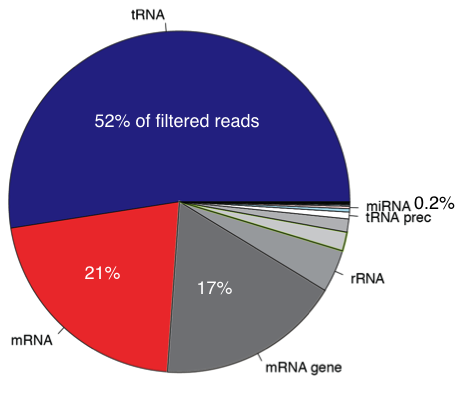
\includegraphics[width=3.5in]{c3po_pie.png}%
\caption[Title.]
{
\textbf{Title.}

}
\centering
\label{c3po_pie}%
\end{figure}

\begin{figure}[!ht]%
\centering
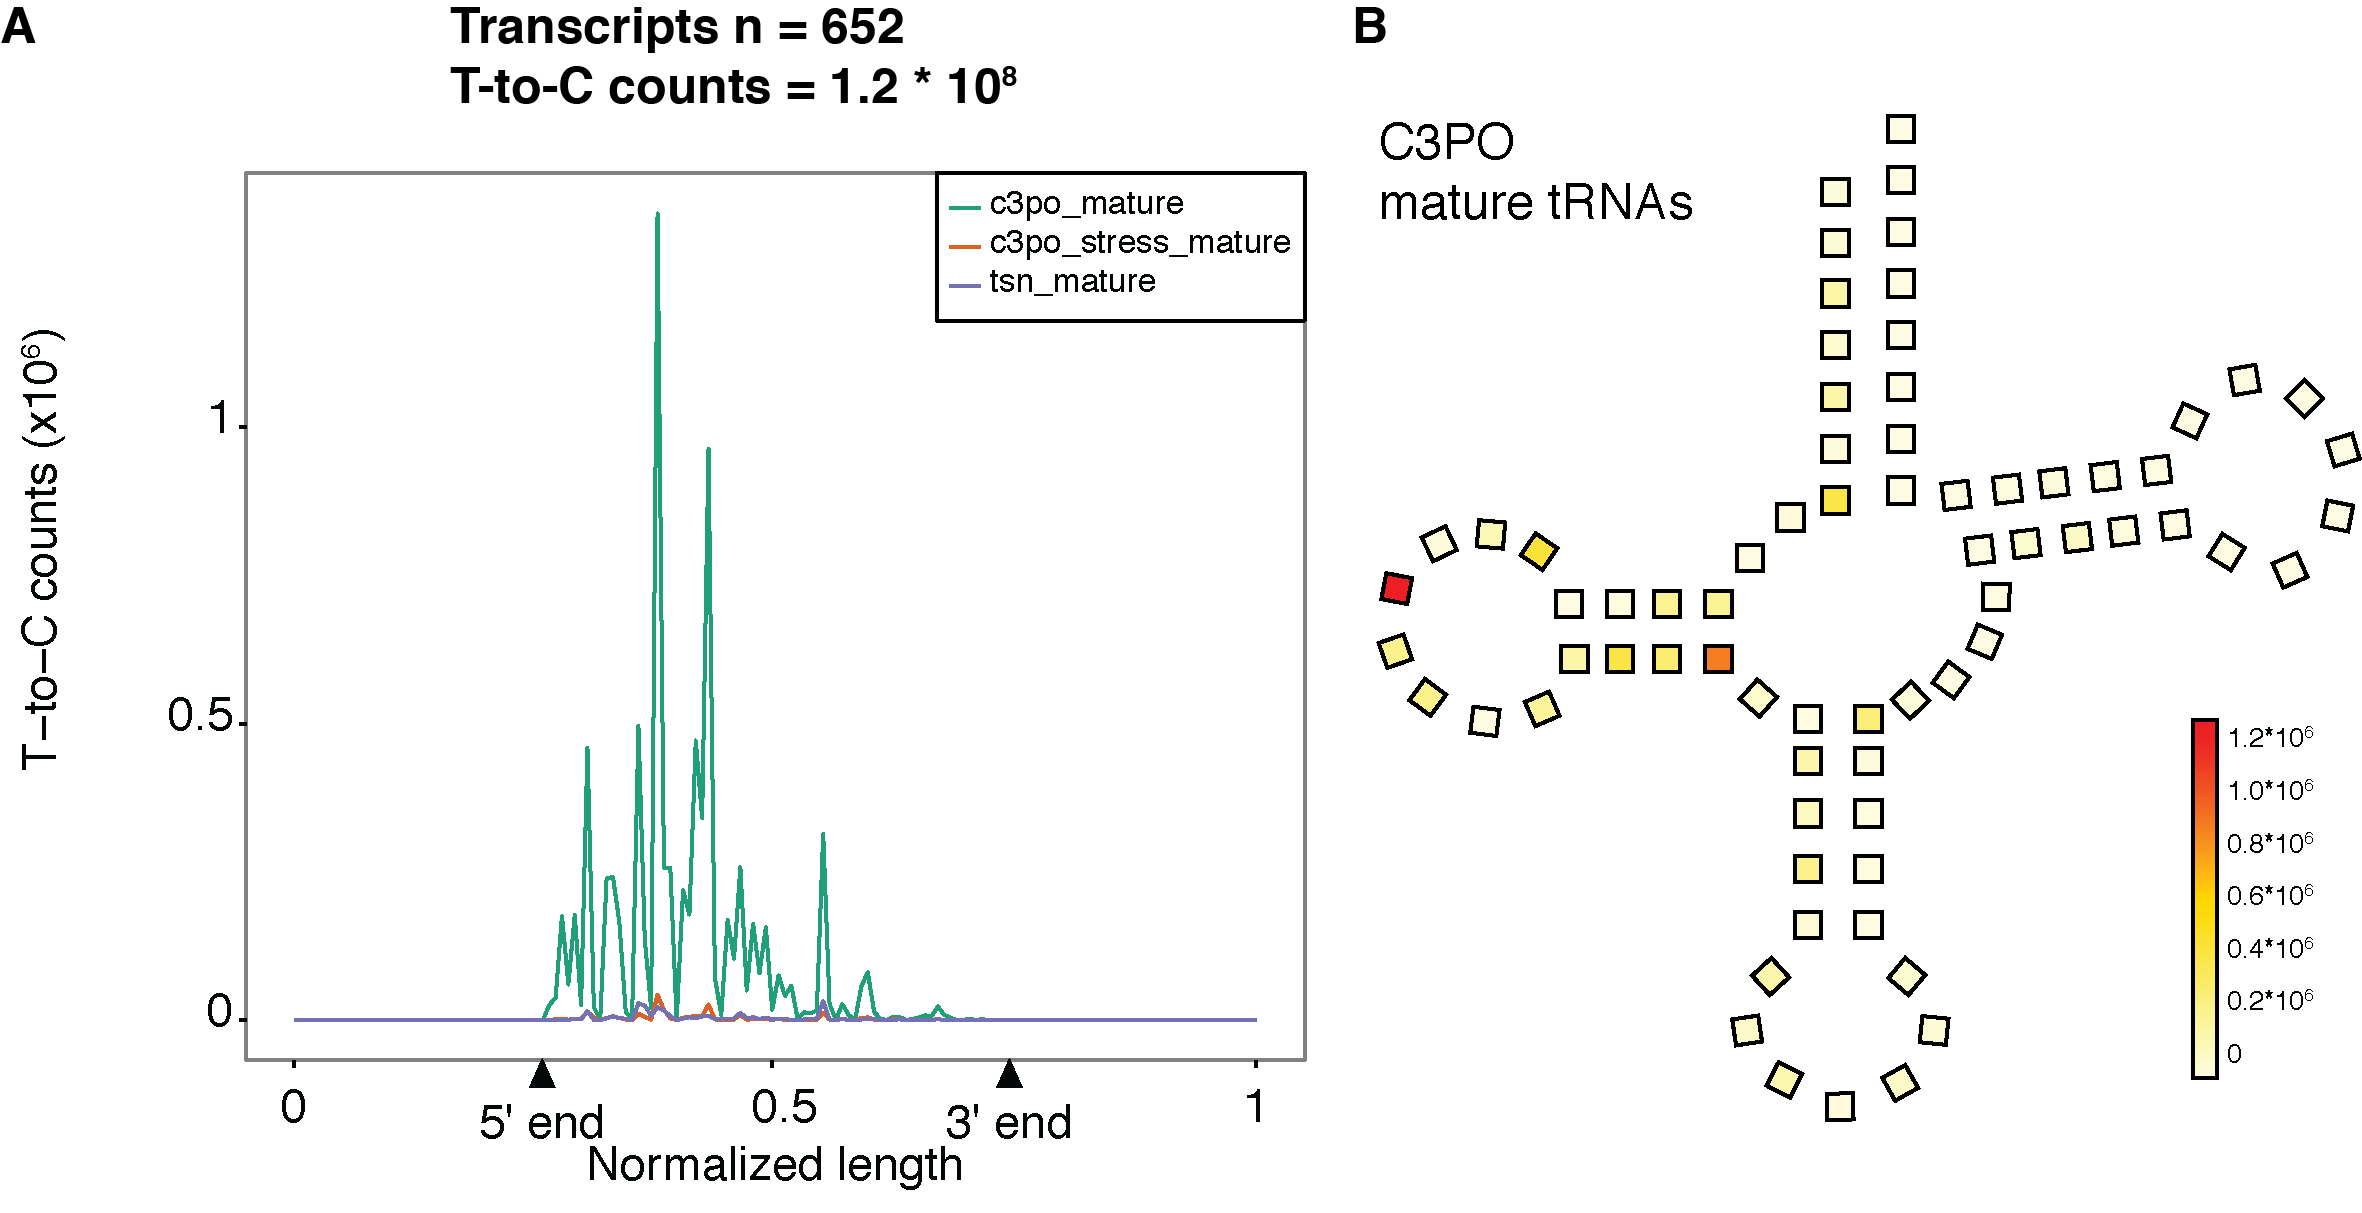
\includegraphics[width=\textwidth]{c3po_pos_dep.png} 
\caption[Metagene analysis of C3PO crosslinking to mature tRNAs.]
{
\textbf{Title.}

}
\centering
\label{c3po_pie}%
\end{figure}

\begin{figure}[!ht]%
\centering
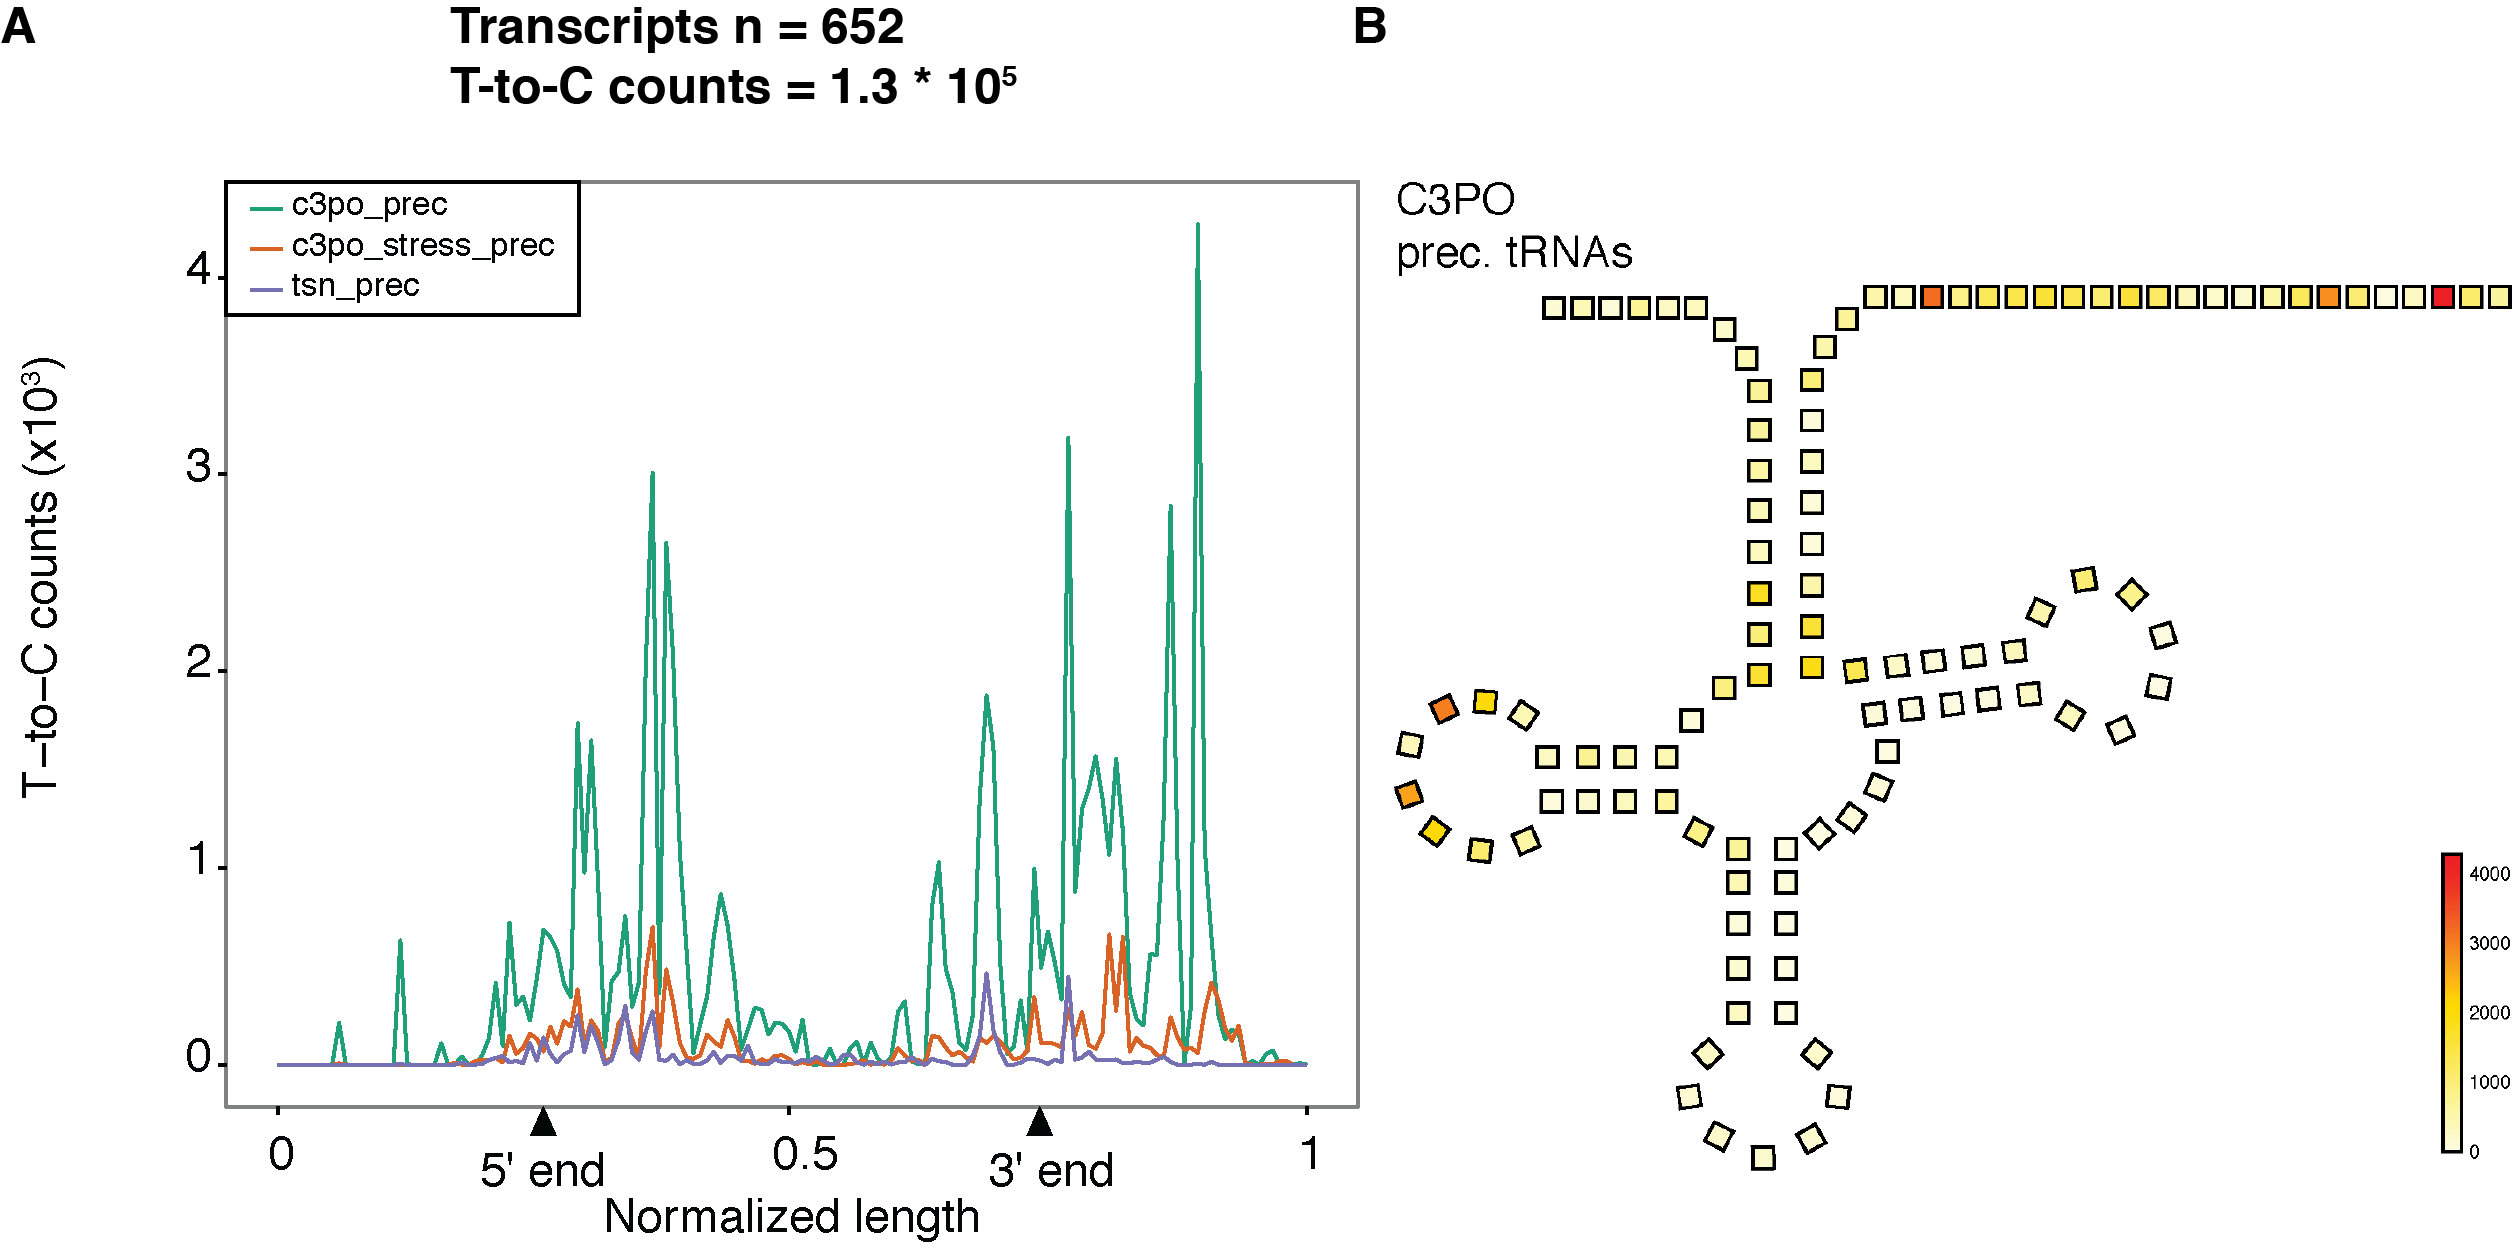
\includegraphics[width=\textwidth]{c3po_pos_dep_pre.png} 
\caption[Metagene analysis of C3PO crosslinking to pre-tRNAs.]
{
\textbf{Title.}

}
\centering
\label{c3po_pie}%
\end{figure}

\begin{figure}[!ht]%
\centering
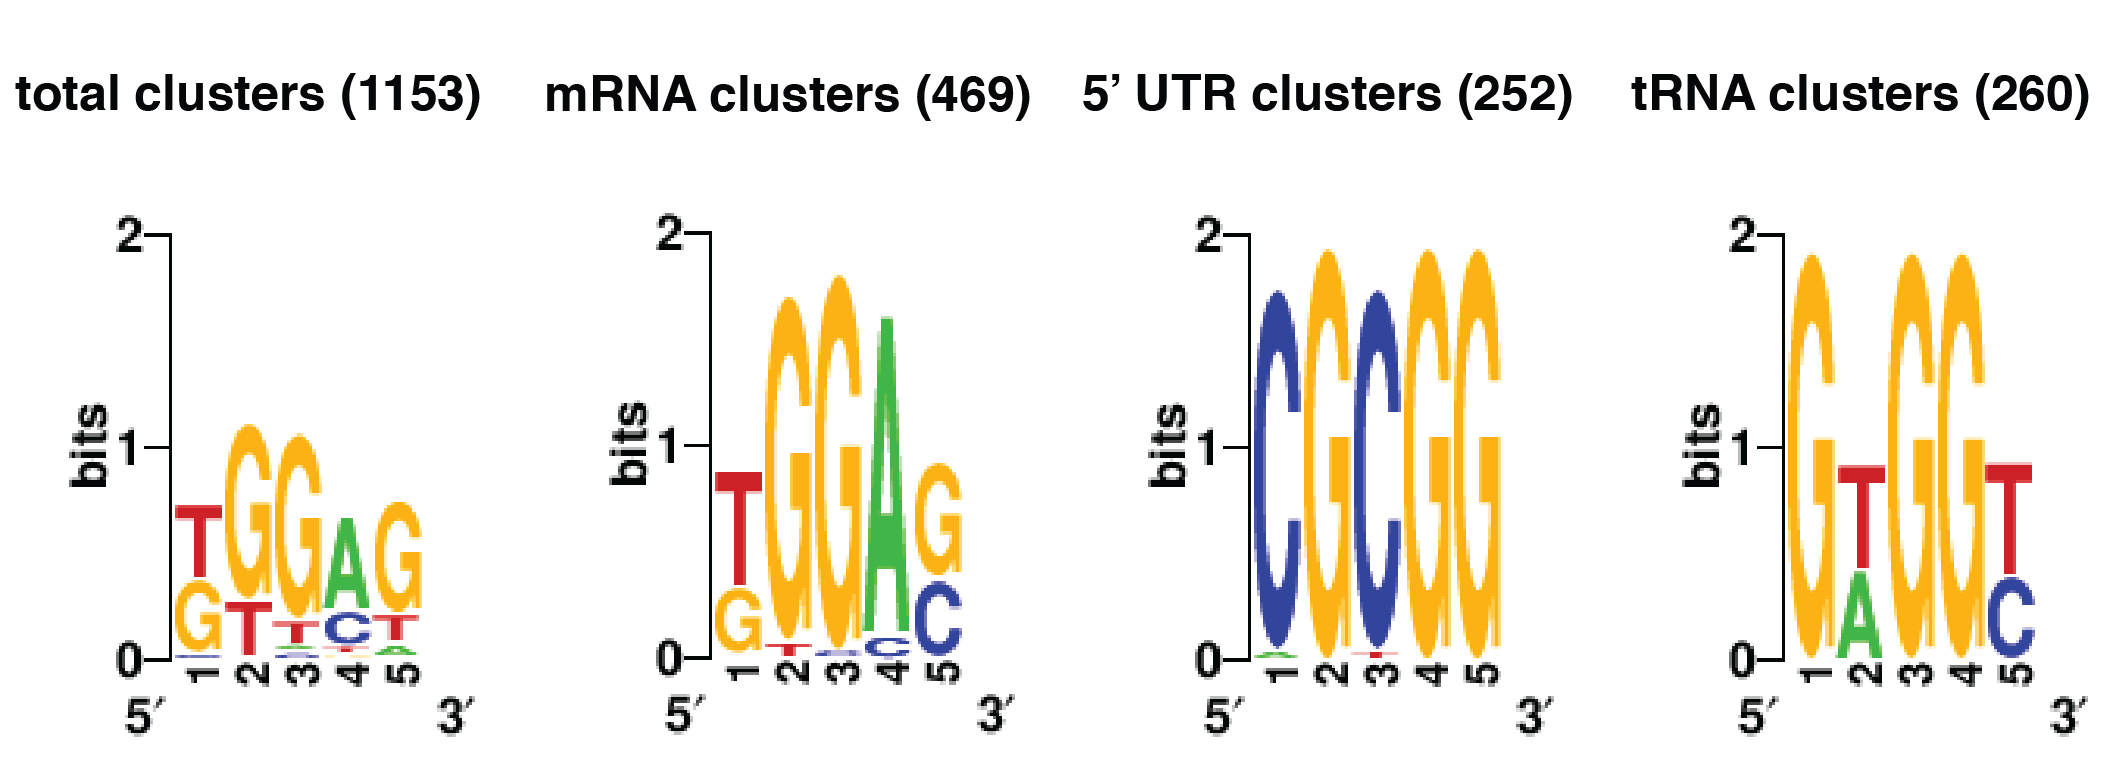
\includegraphics[width=\textwidth]{motifs_collected.png} 
\caption[Motifs.]
{
\textbf{Motifs.}

}
\centering
\label{motifs}%
\end{figure}

\begin{figure}[!ht]%
\centering
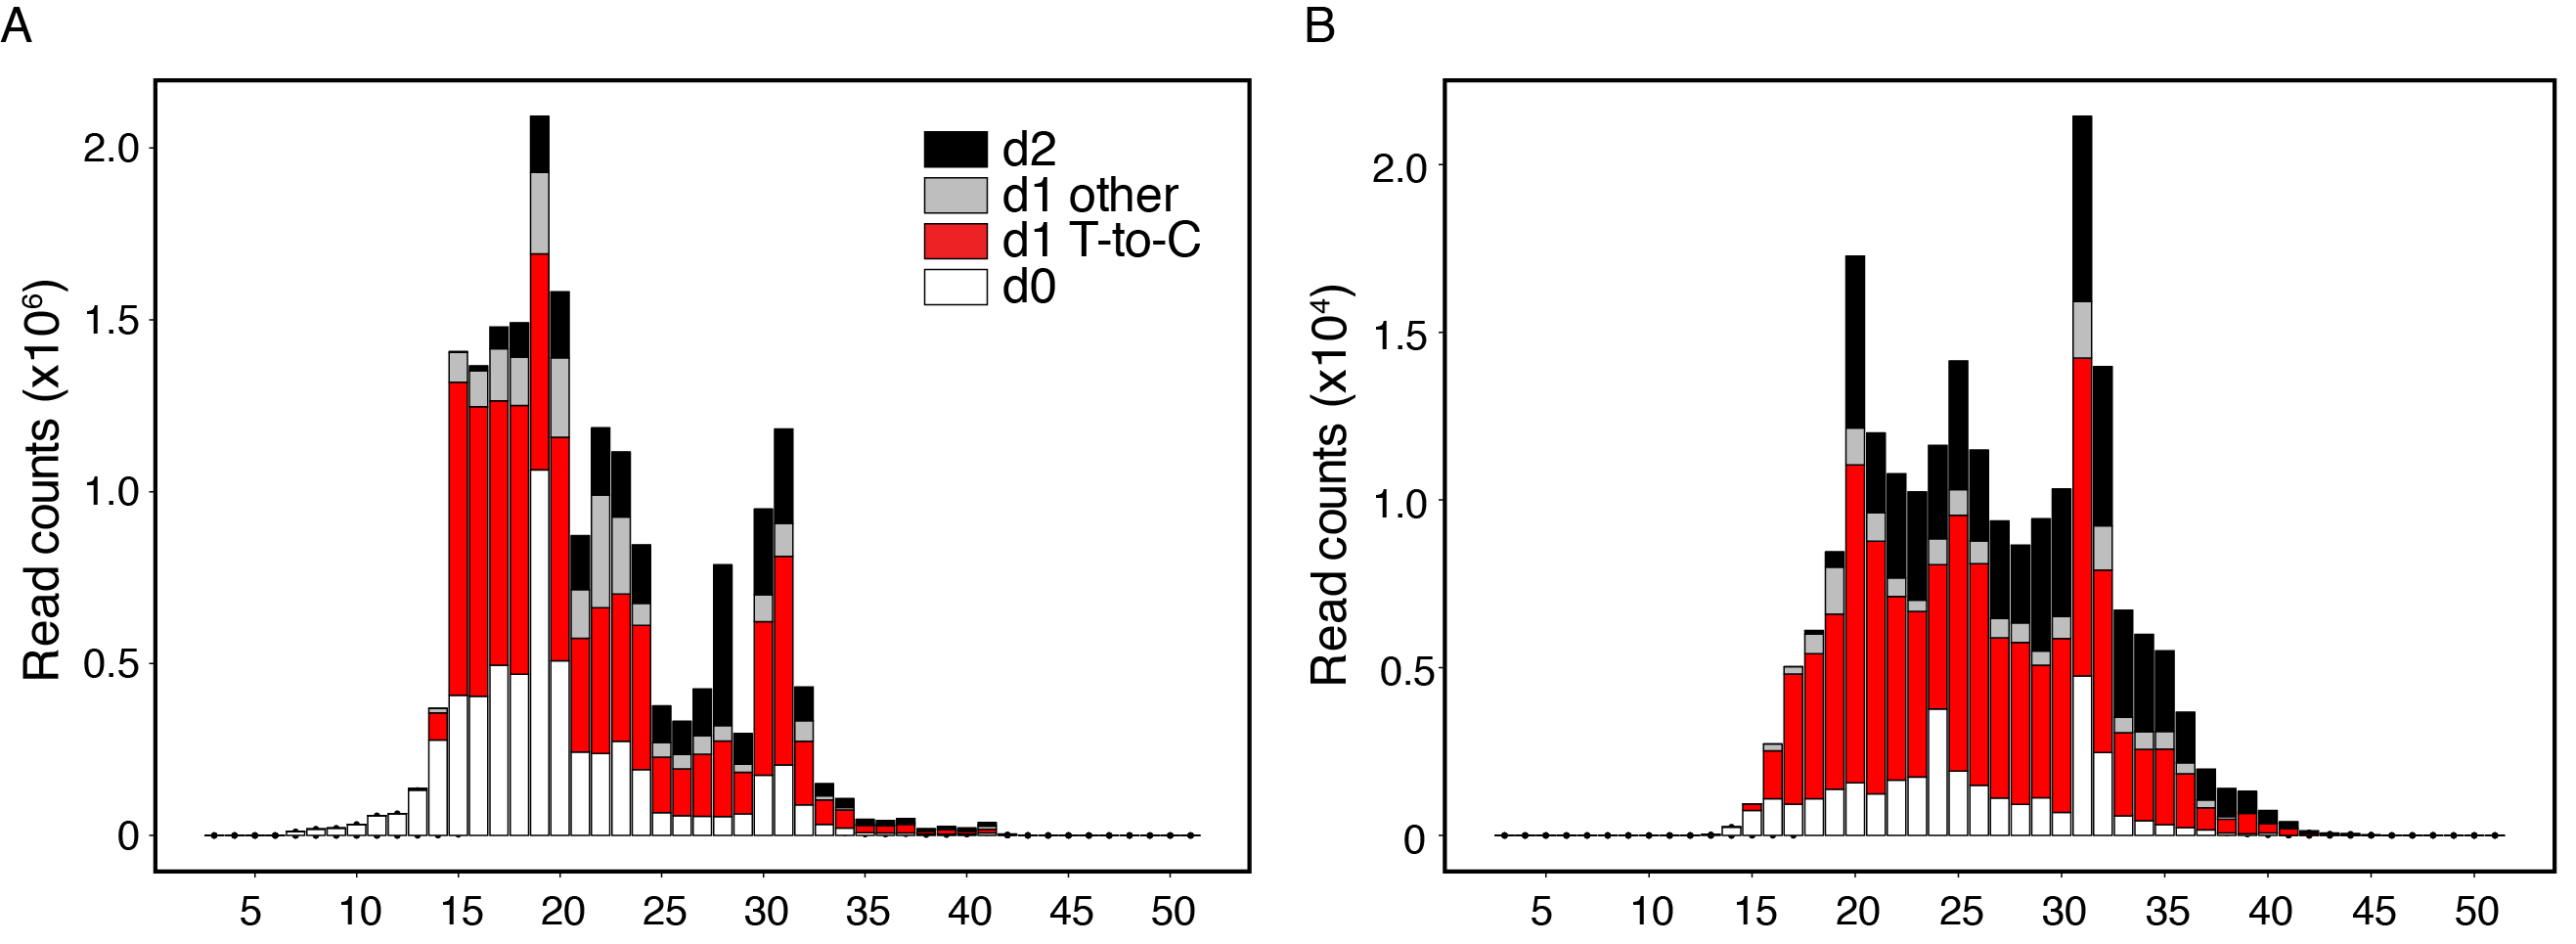
\includegraphics[width=\textwidth]{c3po_pavel.png} 
\caption[Motifs.]
{
\textbf{Motifs.}

}
\centering
\label{motifs}%
\end{figure}

\begin{figure}[!ht]%
\centering
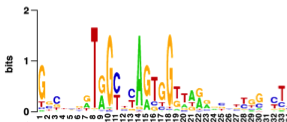
\includegraphics[width=\textwidth]{weblogo.png} 
\caption[Motifs.]
{
\textbf{Motifs.}
see also entropy figure above
}
\centering
\label{motifs}%
\end{figure}

\section{Biochemical characterization}

\subsection{Cleavage activity}

\begin{figure}[!ht]%
\centering
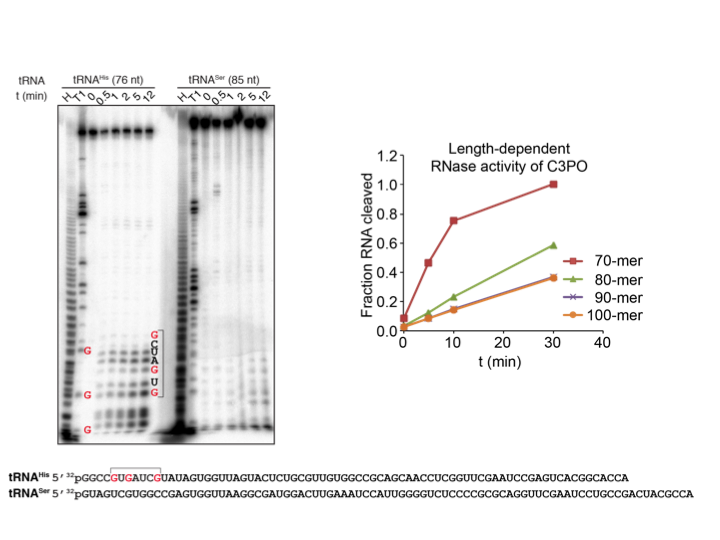
\includegraphics[width=\textwidth]{cleavage2.png} 
\caption[Cleavage.]
{
\textbf{Cleavage.}
see also entropy figure above
}
\centering
\label{motifs}%
\end{figure}

Length and structure dependent cleavage activity

\subsection{EMSAs}
\begin{figure}[!ht]%
\centering
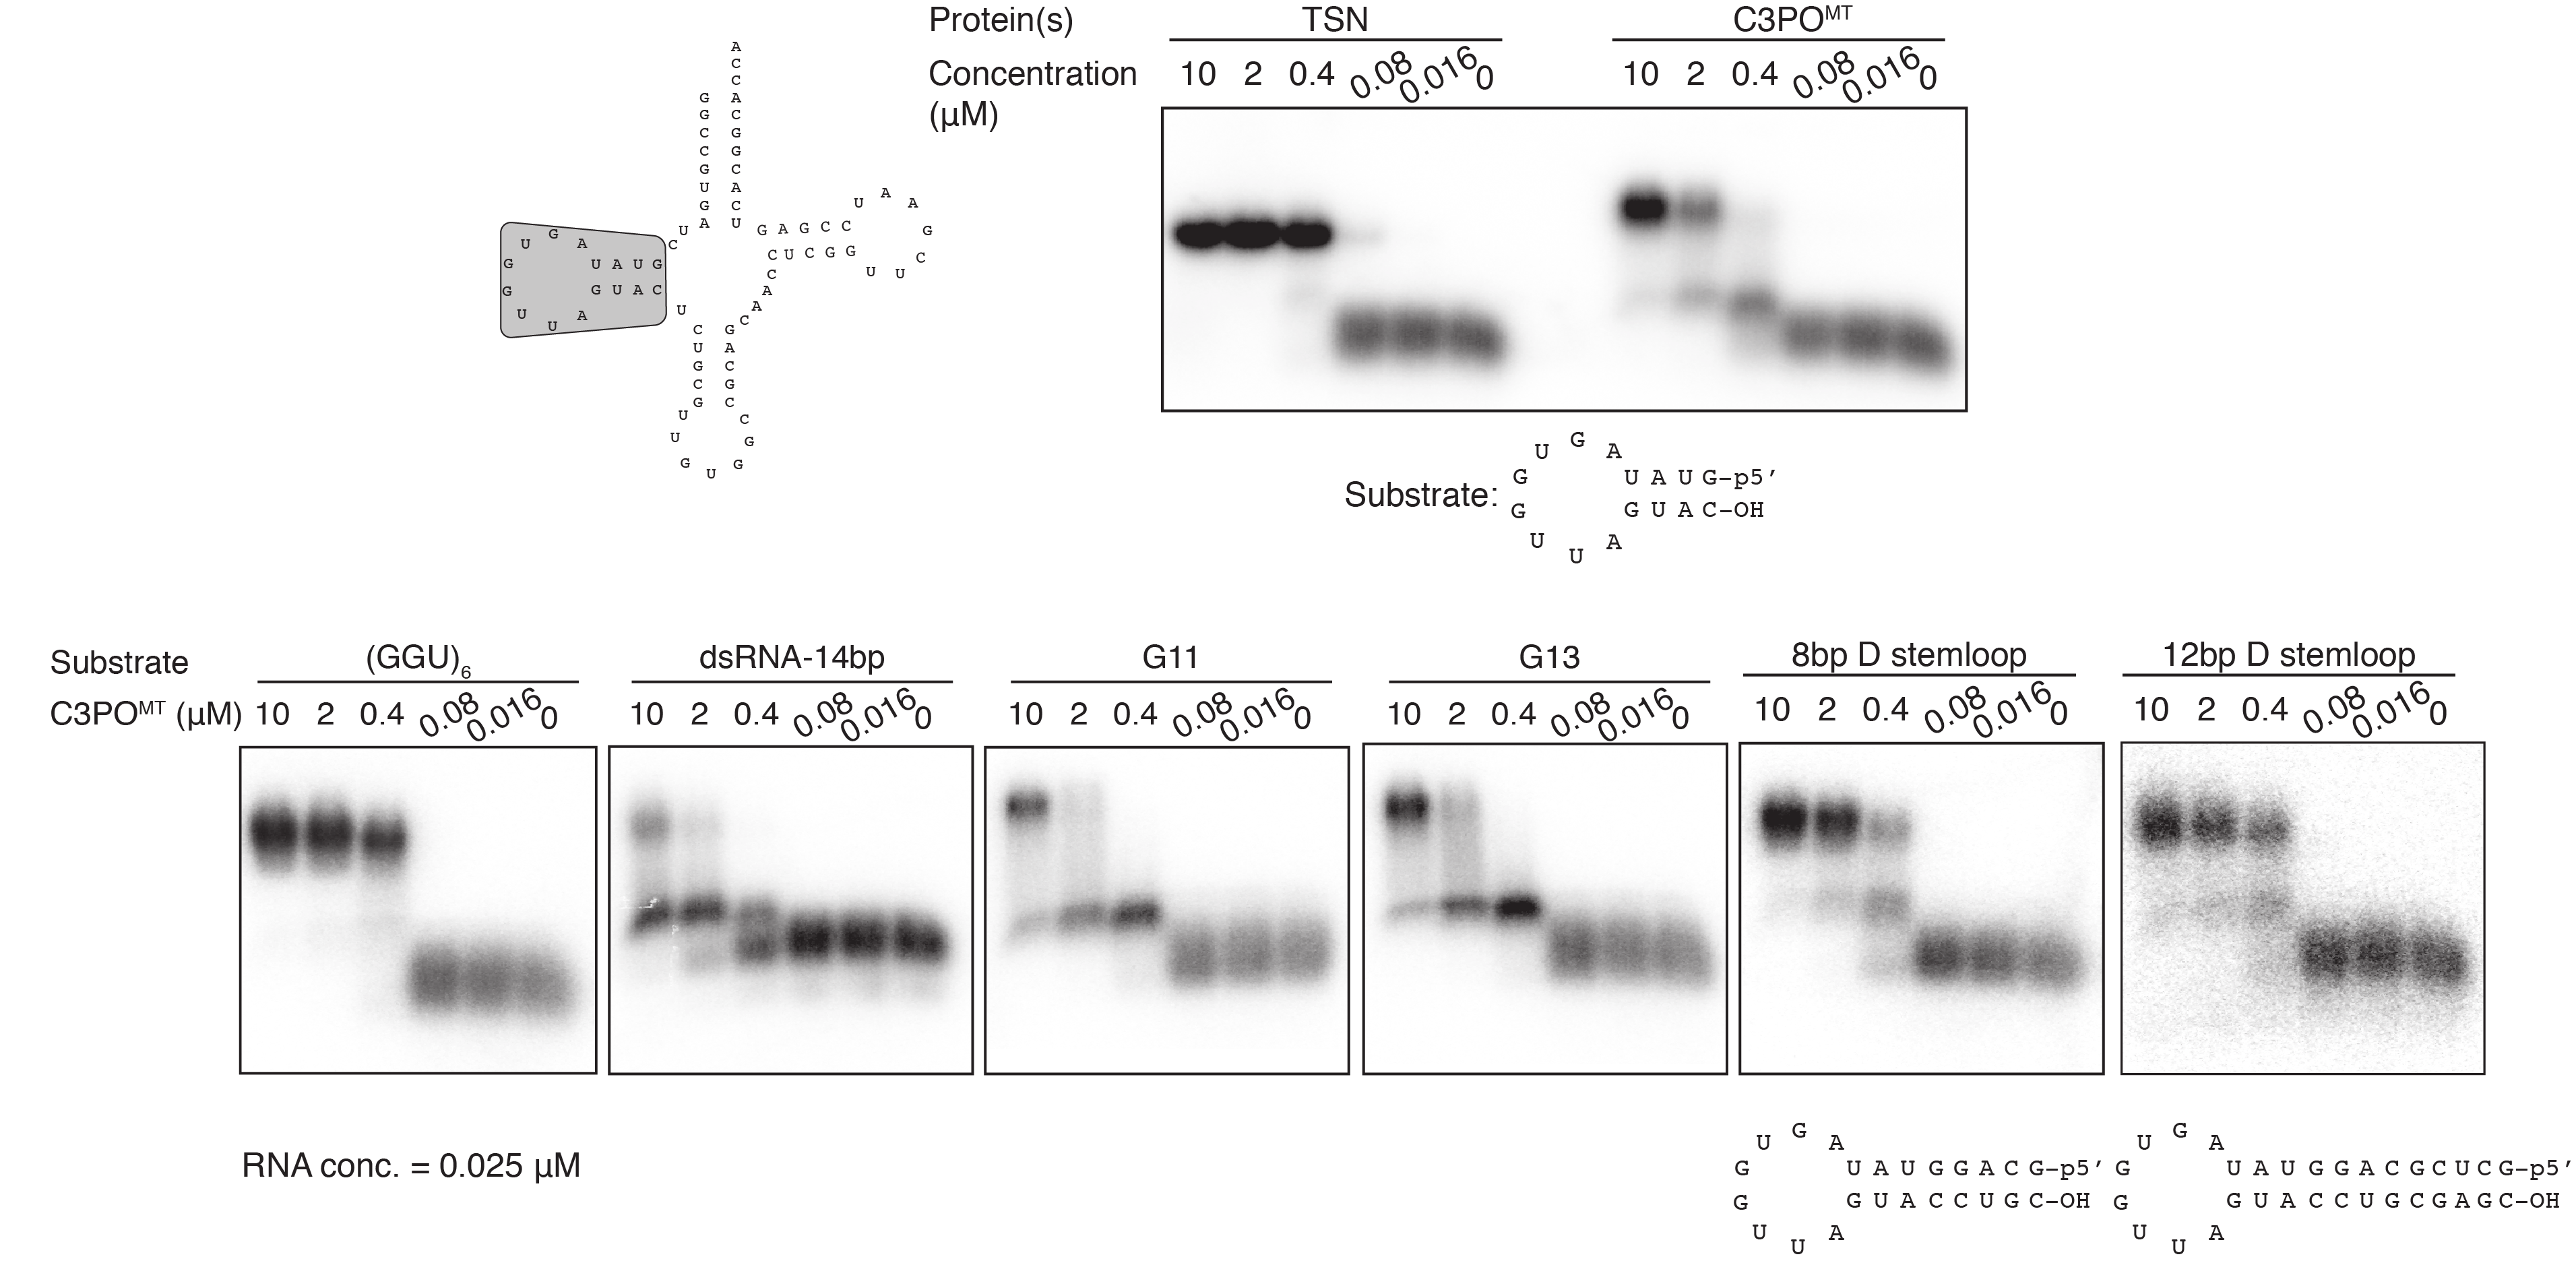
\includegraphics[width=\textwidth]{emsa.png} 
\caption[EMSA.]
{
\textbf{EMSA.}
see also entropy figure above
}
\centering
\label{motifs}%
\end{figure}

\subsection{Structural studies}
only comments

\subsection{Immuno-precipitations}

\begin{figure}[!ht]%
\centering
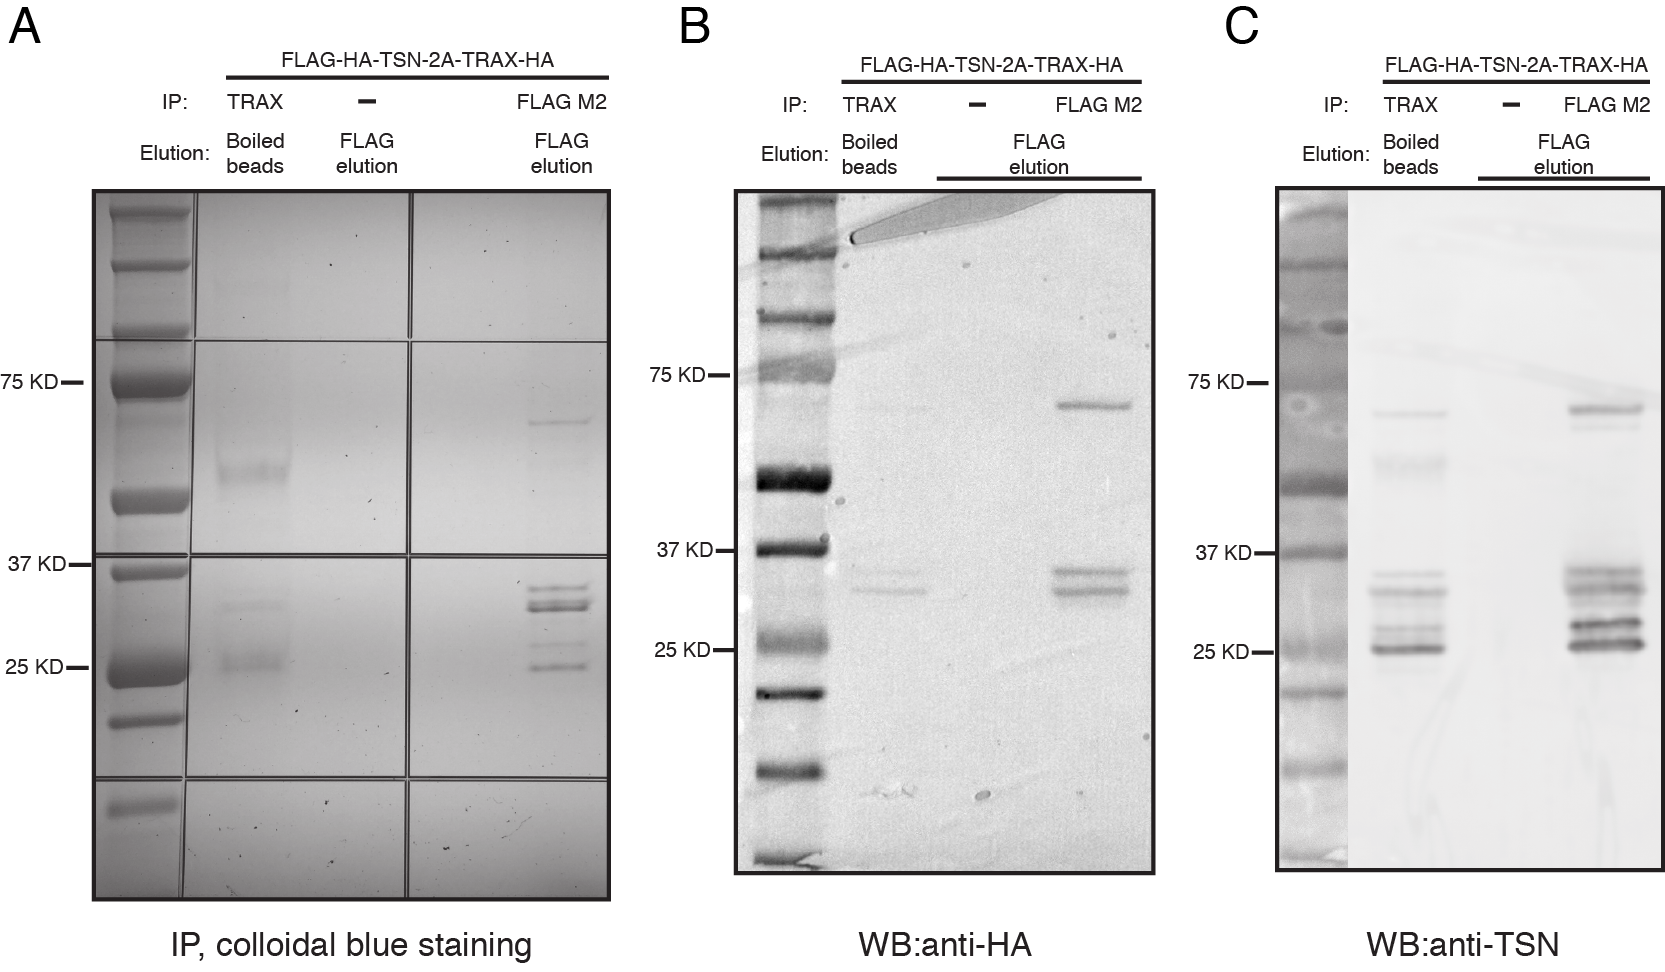
\includegraphics[width=\textwidth]{IP.png} 
\caption[IP.]
{
\textbf{IP.}
see also entropy figure above
}
\centering
\label{motifs}%
\end{figure}


\section{Biological characterization}

  \subsection{Loss of function studies by siRNA knockdowns}

      \subsubsection{hydro-tRNAseq}

\begin{figure}[!ht]%
\centering
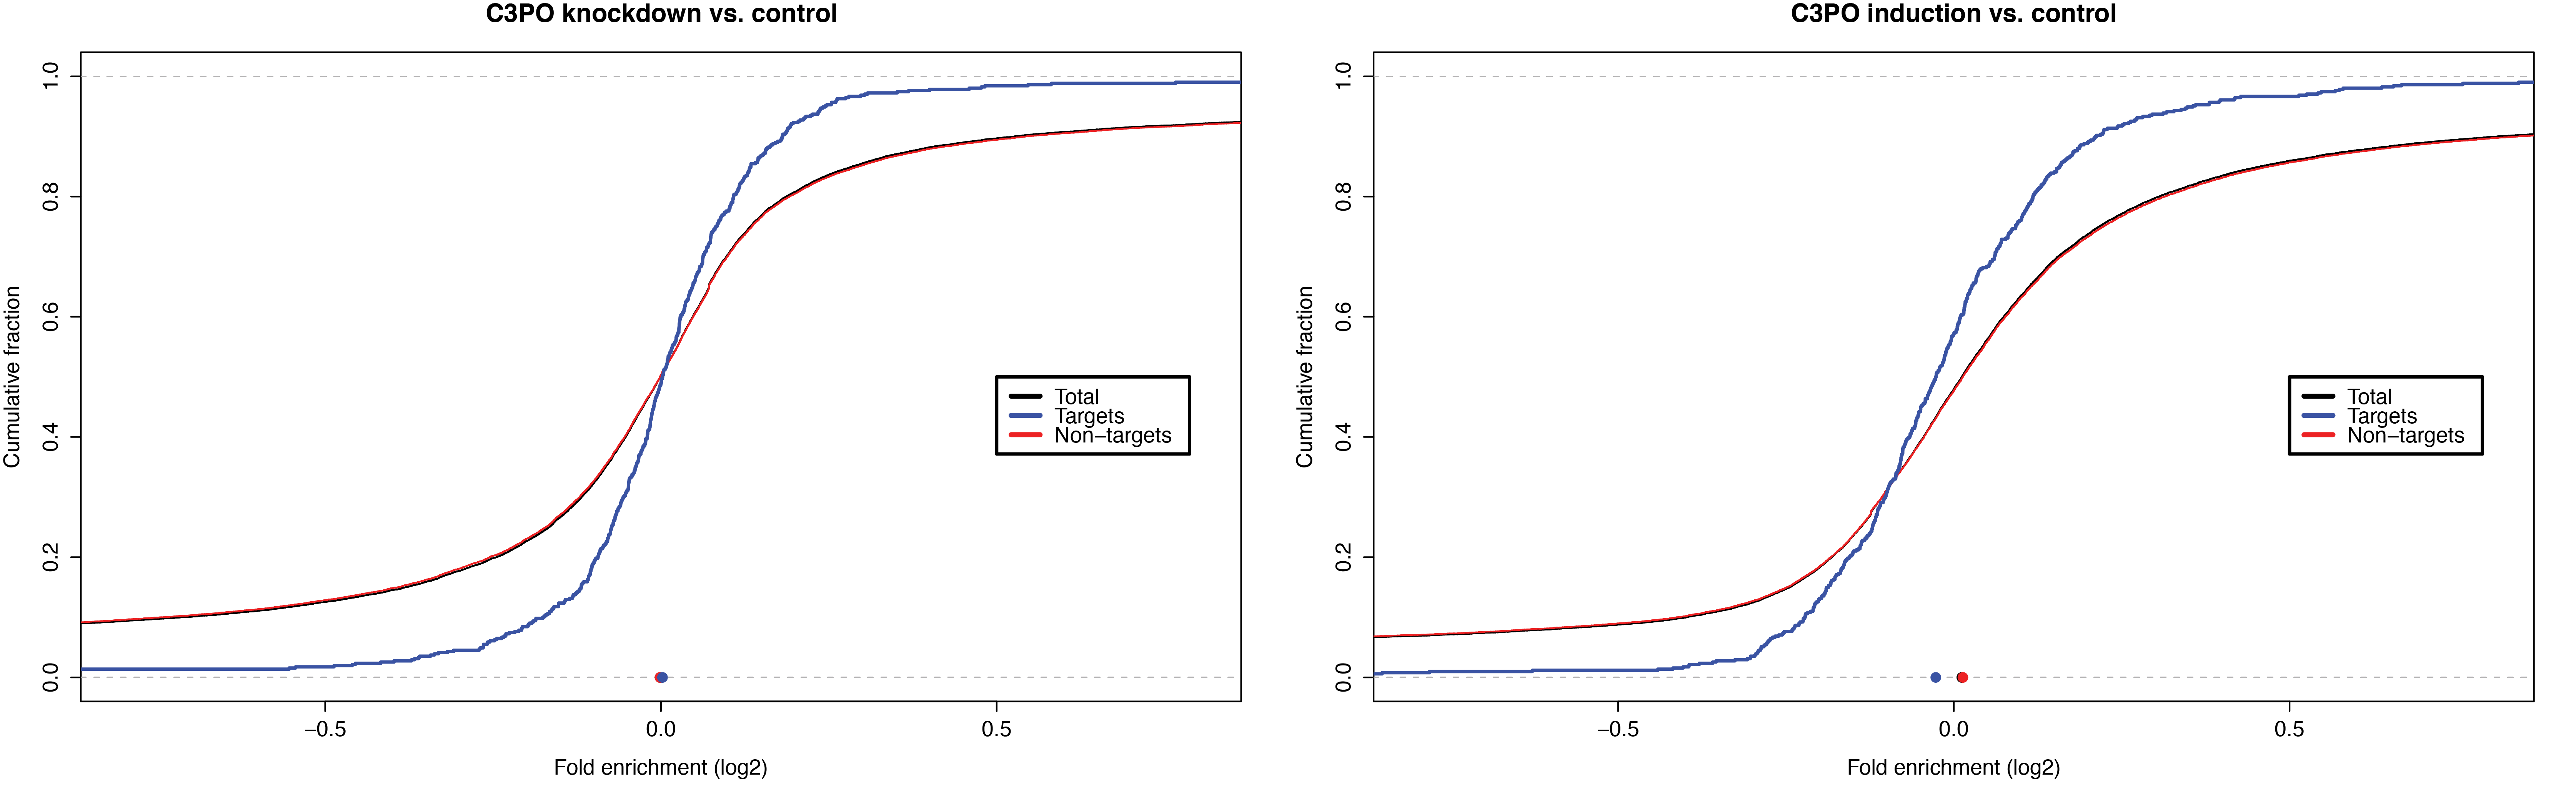
\includegraphics[width=\textwidth]{trnaseq.png} 
\caption[trnaseq.]
{
\textbf{trnaseq.}
see also entropy figure above
}
\centering
\label{motifs}%
\end{figure}

      \subsubsection{mRNA seq}

  \subsection{Translational effects}

  \subsection{Loss of function studies by CRISPR knockouts}

      \subsubsection{mRNAseq}

      \subsubsection{SILAC}

      \subsubsection{Polysome profiles}

\section{Discussion}


\chapter{Materials and methods}
\section{PAR-CLIP}
\section{Cleavage assays}
\section{Immunoprecipitation}
\section{siRNA knockdowns}
\section{CRISPR knockouts}
\section{SILAC}







In both cases tRNA w


	
	We show that C3PO binds to a WGGW motif (W= A or T) in tRNAs and mRNAs. Strikingly, 
	virtually no binding to miRNAs was observed, calling into into question the contribution
	of C3PO to RNAi. 
	

















Recent work from our group and others suggests that C3PO, a multimeric complex of TRANSLIN (TSN) and the nuclease TRANSLIN-ASSOCIATED PROTEIN X (TSNAX), apart from its previously known roles in DNA-damage response and enhancement of RISC activity, possesses also a tRNA processing activity. In agreement with these observations, mutations in the components of C3PO phenocopy mutations in other tRNA processing enzymes by resulting in neurological and behavioral phenotypes54. Also, lack of C3PO activity is associated with accumulation of tRFs10. Thus, it is possible that C3PO might be a regulator of gene expression that could bridge tRNA processing with PTGR. In this aim, I plan to apply the annotated list of tRNAs from aim 1 and the experimental framework for the study of tRNA-tRBP interactions from aim 2 to the study of C3PO, a regulator of gene expression that could possibly provide a new bridge between tRNA processing and PTGR. 

C3PO notes. TRANSLIN (TSN) was initially described as a protein that would bind DNA breakpoint junctions at conserved sequences. Initial studies identified that TSN was specifically localized in the nucleus of lymphoid cell lines, suggesting that it might play a role in DNA repair, replication or recombination (Aoki et al. 1994, 1995). 

TSN contains five potential protein kinase C phosphorylation sites, three tyrosine kinase phosphorylation sites (Aoki et al. 1995).
TSN was detected in the cytosolic fraction of nonlymphoid and lymphoid cells, and in the nuclear extract of lymphoid cells. It was also detected with a slightly faster mobility in non-hematopoetic cells (e.g. HeLa). 
In conclusion, the nuclear relocalization of TSN is “selectively controlledin lymphoid lineage cells”. 

In this study, TSN was identified as a ssDNA binding protein that binds conserved sequences at the breakpoint junctions in lymphoid cells that have undergone DNA translocations. A proposed role for TSN binding of these DNA loci was “DNA-unwinding, which makes these regions more susceptible to nuclease cleavage.”

“Since DNase I or S1 nuclease hypersensitive sites were observed near these breakpoints, and potential Z-DNA elements have been shown to be important in homologous recombination, it is conceivable that the above DNA structures influence chromatin structure and render a localized region of DNA more accessible to recombinase.”

“These results raise the intriguing possibility that a mechanism of active nuclear transport for TSN exists and that TSN might be associated with lymphoid specific processes, such as Ig/TCR rearrangement.”

Regarding the cytosolic function of TSN in non-lymphoid cells “one possibility is that, analogous to RecA protein, TSN may be required for repair of DNA damage caused by radiation or chemicals.”

The high expression pattern of TSN in testes, a tissue that is know to undergo extensive DNA rearrangements provides further evidence that the protein may be involved in DNA damage control. 

\begin{figure}[!ht]%
\centering
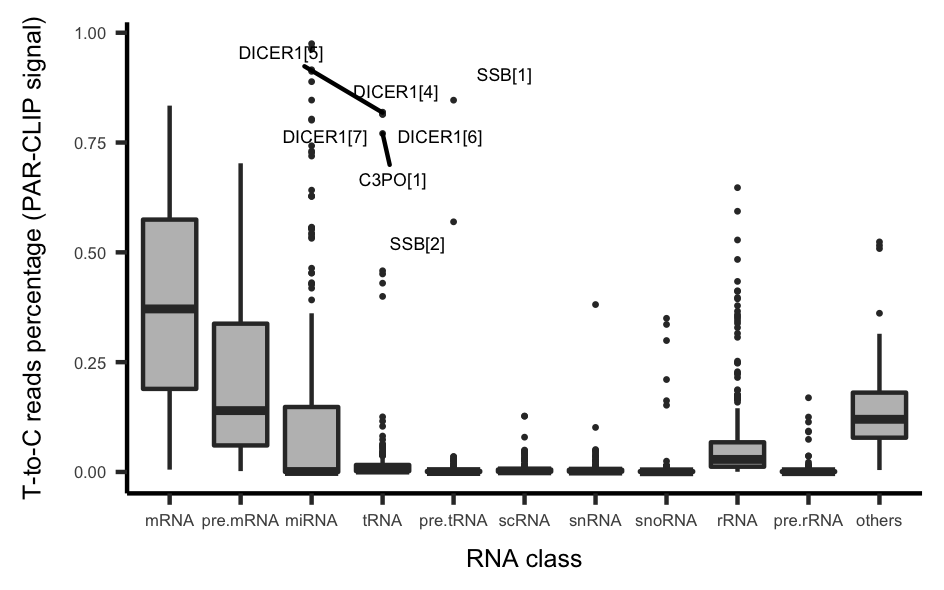
\includegraphics[width = \textwidth]{parclips.png}%
\caption[parclips]
{\textbf{parclips.}
placeholder}
\centering
\label{parclips}%
\end{figure}

\section{From manny}
C3PO is an RNA/DNA-binding protein complex of TRANSLIN (TSN) and TRANSLIN-ASSOCIATED FACTOR X (TSNAX), which was originally reported to co-localize with breakpoint junctions of chromosomal translocations. Tsn-/- mice were created with the hypothesis that its absence would affect genome stability. Interestingly, mice lacking Tsn exhibited learning and memory defects indicating that it is necessary for brain development or neurological maintenance. C3PO was recently reported to enhance RNAi activity in Drosophila and humans, wherein TSNAX possessed a novel and highly conserved ribonucleolytic activity. In collaboration with Dinshaw Patel’s group (MSKCC), I biochemically characterized its nuclease activity and we solved the structure of Drosophila C3PO. Concurrently, the Liu laboratory (UTSW) crystallized human C3PO. Despite these recent efforts, neither the endogenous targets nor the mechanism of C3PO assembly and nuclease activity are well understood. Given the positions of the nuclease catalytic sites, it is not clear if C3PO dynamically assembles onto its substrates, or if RNA molecules are fed inside the structure.

I have biochemical data showing that human and Drosophila C3PO possess a length-dependent ribonuclease activity (Fig. 4). C3PO nuclease activity is much reduced for RNA substrates >80 nt. The physiological importance of the length-dependent activity is not known, though one clue may come from a recent publication on a newly reported function of C3PO regarding maturation of tRNAs, which are typically between 70 and 90 nt in length. Independently, Andrew Fire and colleagues recently described small RNAs derived from tRNAs as a potential class of non-coding RNA regulators of RNA-induced silencing complex (RISC) activity. Given its purported roles in RNAi and tRNA maturation, it is tempting to hypothesize that C3PO fulfills aspects of both independently described mechanisms. Consistent with this working hypothesis, I find high crosslink evidence within the D-arm of tRNAs from a TSN PAR-CLIP (Fig. 5). These results indicate that TSN associates with specific tRNA hairpin loops containing an invariant sequence, a sequence I also find in the mRNAs that TSN binds. I plan to determine and characterize the endogenous RNA substrates of TSN and C3PO. Since TSN can form multimeric complexes without TSNAX it is plausible that specific RNAs are binding targets of only TSN, as opposed to the C3PO complex. As the relationship between TSN-only vs. C3PO complexes is not well characterized, I have created stable cell lines that express TSN, TSNAX, or the entire C3PO complex in an effort to determine whether there are target overlaps between the two types of TSN complexes. I will biochemically validate the RNA-protein interactions identified, prioritize these targets by determining TSN or C3PO enrichment with RNAs and develop assays that, depending on the RNA category, functionally define the role of TSN and/or TSNAX. I will initially focus on assays that investigate RNA stability, RISC-dependence, and tRNA involvement, since these areas reflect the current understanding in the field. In future studies, I plan to characterize C3PO-containing mRNP and tRNP complexes in order to better understand its role among other PTGR components and processes.

\section{TSN binds tRNAs}
Our laboratory has identified a limited set of the RNA targets of human C3PO by performing PAR-CLIP analysis of its components. Expression of TSNAX alone did not yield any crosslinked RNAs – presumably due to its nuclease activity. However, PAR-CLIP with TSN did yield crosslinked RNAs. Preliminary analysis of this dataset shows that TSN exhibits high crosslinking efficiency to tRNAs, as well as mRNAs. In particular its consensus targets include the conserved UGGU motif of the dihydrouracil (DHU) stem-loop of tRNAs. A similar motif is also observed in the most prominent mRNA targets of TSN (Figure 5).

\section{C3PO possesses a length- and structure-dependent endonucleolytic activity}
%We have previously observed that the endonucleolytic activity of C3PO is much reduced for RNA substrates longer than 80-nt (unpublished data). This cutoff is very close to the average length of a mature human tRNA ( 75 nts). The length cut-off of C3PO’s activity along with the presence of tRNAs in its PAR-CLIP target list prompted the in vitro study of C3PO’s nuclease activity on tRNAs. I performed cleavage assays on 5’ or 3’ labeled, in vitro transcribed histidyl-tRNA (tRNAHis, 76 nts) and seryl-tRNA (tRNASer, 85 nts) (Figure 6). These substrates were chosen because of their confirmed presence in the TSN PAR-CLIP dataset, and because they lie inside and outside the length-dependent window of optimum nuclease activity respectively. My data suggest that tRNAHis is a favored substrate, consistent with the length preference of C3PO. More importantly I have noticed that C3PO possesses a structure-dependent cleavage pattern with respect to tRNAs. C3PO activity does not lead to processive degradation of the tRNA substrates (see H in figure 6), but rather results in products of specific length (\leq 9 nts). This suggests that C3PO cleaves preferentially at the shoulders of the acceptor stem of tRNAs, providing a possible cleavage site for the production of tRFs. 

\section{Biochemical characterization of C3PO’s tRNA processing activity}
I plan to repeat the PAR-CLIP analysis of TSN, using the tools and expertise obtained from aims 1 and 2 in order to validate its interaction with tRNAs. At the same time, in order to gain insight into the substrates of the full complex, I plan to perform PAR-CLIP studies after co-expression of TSN with a catalytically inactive form of TSNAX, due to a single amino acid mutation at its active site40. Based on structural studies, a catalytically inactive TSNAX is expected to form a similar stoichiometric complex with TSN as its wild-type form and bind its natural RNA targets, without being able to cleave them, thereby allowing their identification by PAR-CLIP. The targets identified by PAR-CLIP will be validated, in part, by in vitro nuclease assays so as to determine the details of the catalytic mechanism of C3PO on its substrates. 

\section{Functional validation of C3PO’s targets}
The impact of C3PO’s activity on its targets will be examined in over-expression and knockdown experiments. I plan to perform HydroRNAseq and RIP-Seq studies to investigate the impact of C3PO expression levels on the stability of its RNA targets, and to further dissect its biological function. Lack of C3PO activity has been linked with elevated levels of mature tRNAs and pre-tRNA fragments10. At the same time, C3PO activity is suggested to promote activity of RISC leading to enhanced RNA silencing38. If the former in the true, I expect to observe an accumulation of pre-tRFs and mature tRNAs in knockdown versus control or over-expression. If the latter holds, then I expect a change in the stability of the mRNA targets of C3PO. Finally, if time permits, I intend to study the effect of C3PO’s activity on the protein level, by performing western blot and mass-spectrometry studies of the proteins whose mRNAs will be validated targets. 

\section{C3PO sumary report 2014}
Performing PAR-CLIP on C3PO confirmed its role as a bona fide tRNA binding protein. The evidence for this is twofold: a) tRNAs collect the largest number of sequenced reads, 31\%, with the 2nd most represented class, mRNAs, collecting only 9\% (table 1), b) tRNAs represent the largest percentage of PAR-CLIP clusters both within the total number of clusters, as well as within the top 100 clusters (ranked by read abundance) (figures 1, 2, table 2). Of note, my PAR-CLIP results seem to bring into question previous reports that implicated C3PO in enhancing RISC activity and promoting miRNA-mediated gene silencing, since only 4\% of the total clusters map to miRNA and 3’ UTRs, respectively (table 2). However, 5’ UTRs represent 22\% of all clusters, a result that comes as a surprise, as C3PO has not been reported to interact with 5’ UTRs before. I have also determined the tRNA binding motif of C3PO (figure 3), using motif prediction algorithms (GIMSAN and MEME). Currently I am carrying out RIP-seq experiments in order to validate and rank the targets of C3PO.

In order to investigate the biochemical function of C3PO, I am trying to identify other interacting proteins. A preliminary co-immunoprecipitation analysis yielded no clear candidates, which suggests that either C3PO functions in no close association with any other protein or that the conditions of immunoprecipitation were not appropriate. At the moment, I am repeating the experiment at different salt concentrations, as well as in the presence of a cell-permeable crosslinking agent (DSP). I hope that in this way I will be able to stabilize the possible interactions of C3PO with other proteins, which I will then identify by using the mass-spectrometry core facility. Moreover, I have already carried out in vitro endonuclease cleavage assays, using recombinant C3PO. These experiments confirmed that C3PO cleaves in vitro transcribed tRNAs in a length- and structure-dependent manner. I will carry out similar studies using tRNA targets predicted from PAR-CLIP and confirmed by RIP-seq. 

Since C3PO has been previously implicated in a plethora of biological processes, I am interested in elucidating the processes in which it partakes. For this purpose, I am carrying out a gene ontology analysis of the PAR-CLIP targets. Also, I have performed siRNA knockdown experiments against the two components of the C3PO complex, TSN and TSNAX. I have validated commercially available antibodies, designed siRNAs, and have successfully knocked down C3PO in HEK293 cells by 3- to 5-fold. As the next step, I will perform two series of RNA-sequencing experiments in the context of C3PO knockdown: mRNA-seq (poly A selection) and HydroRNAseq, to determine the effect of C3PO expression on the mRNA and tRNA population, respectively. 

Finally, a series of reports implicate tRNA metabolism in stress responses. Specifically, it has been suggested that upon cellular damage, tRNA endonucleolytic cleavage leads to translational arrest via the accumulation of tRNA halves. I subjected HEK293 cells to treatment with sodium arsenite (an inducer of oxidative stress), isolated RNA, and then performed small RNA sequencing that confirmed the accumulation of stable 5’ tRNA fragments. As a control, the miRNA or snRNA population remained largely unchanged. I confirmed these results by northern blots. Stress-induced endonucleolytic cleavage of tRNAs has been reported to be a function of the nuclease angiogenin. Nevertheless, angiogenin is not appreciably expressed in our cell culture system, neither in normal growth conditions nor upon oxidative stress. Therefore, it is intriguing to assume that C3PO might play a previously uncharacterized role in the metabolism of tRNAs during stress. For this purpose, I have carried out a PAR-CLIP experiment under conditions of oxidative stress and I am currently awaiting the sequencing results. 

\section{C3PO summary from annual report 2015}
C3PO is a multimeric complex of the RNA binding protein TRANSLIN and the RNA endonuclease TRAX. A plethora of functions have been assigned to this complex, such as a role in the repair of DNA breaks, enhancement of RNAi activity, and tRNA processing. By performing PAR-CLIP I had previously identified C3PO as a tRNA binding protein, and showed that it does not bind to miRNAs or 3’UTRs of mRNAs, arguing against a role in RNAi. Except for tRNAs, the other main target of C3PO was 5’ UTRs, something unusual for mRNA binding proteins apart from translation initiation factors. 

In order to investigate the effect of C3PO in mRNA and tRNA stability, I performed mRNA and tRNAseq upon knockdown as well as induction of C3PO. To my surprise no significant effect was observed in either class of RNAs. There results can be interpreted in two ways. First, since C3PO is an enzymatic complex, perhaps partial loss of function conferred by siRNA knockdown is not sufficient to yield an observable phenotype, at least under the tested experimental conditions. Second, C3PO has an effect on translation rather than on mRNA or tRNA stability. I am testing the former hypothesis, by performing sequencing on RNA isolated from Translin and Trax knockout flies, and the latter by performing polysome analysis and mRNA reporter translation assays. Finally, in order to elucidate the molecular mechanism of action by C3PO, I have engaged in a collaboration with the lab of Dinshaw Patel at MSK, trying to obtain a crystal structure of C3PO with a minimal or full-length RNA target identified in my PAR-CLIP analysis. 

\section{C3PO summary from annual report 2016}
Despite extensive efforts in collaboration with the Patel lab (MSK), we have not been able to obtain a crystal structure of C3PO (complex of TRANSLIN and TRAX) bound to its RNA targets, which I have previously identified by PAR-CLIP. I have performed extensive electrophoretic mobility shift assays that have specified optimal substrates (e.g. full length tRNA, single stranded GGU repeats of various lengths, short RNA stemloops containing C3PO’s putative binding motif TGGW - W= A or T). Using these substrates, the Patel group obtained well-diffracted crystals of TRANSLIN crystallized in presence of ether single stranded RNA sequence 5’-(UG)3U(UG) or the tRNA dihydrouridine stem loop sequence (5’-GUAUAGUGGUUAGUAC) that belong to two different space groups. The structures were solved at 2.2 Å and 2.74 Å resolutions, respectively, and revealed minor differences in the arrangement of octameric TRANSLIN, but no bound RNA substrate in the expanded hollow interior of the closed-barrel structures. They have also obtained small crystals of the truncated wild-type C3PO in the RNA-free state, which are currently being optimized to attain diffraction quality.
	
In parallel, I have been characterizing the in vivo effects of C3PO, by loss-of-function studies. Unexpectedly, I observed that siRNA knockdowns of TRANSLIN led to increased translation of mRNA targets identified by PAR-CLIP. At the same time, more than 30 ribosomal proteins were upregulated upon TRANSLIN knockdown. Therefore, there is evidence that C3PO has a role in regulating translational efficiency. I have confirmed by RNAseq that C3PO is ubiquitously expressed at moderate to high levels. Therefore, there are reasons to think that C3PO might be involved in fundamental and global regulation of translation, either by acting directly at the translational process or indirectly, by modulating tRNA levels. In fact, the binding properties of C3PO towards specific 5’ UTRs of some mRNAs reflect those of known translational factors, inasmuch as they are usually single, short binding sites with GC-content significantly higher than randomly sampled, size-matched sequences from the 5’ UTR background context19.

Since TRANSLIN knockdowns did not have a global pronounced effect on tRNA levels, I reasoned that the depletion achieved by the siRNA methodology (~70\% reduction in protein level) was not impactful enough to result in an observable effect on global tRNA levels. Therefore, I am obtaining CRIPSR knockouts20 of TRANSLIN and TRAX, which I will start characterizing after the submission of my tRNA manuscript.

Although previous attempts to co-immunoprecipitate (co-IP) interactors of C3PO had been fruitless, I have optimized the IP conditions, managing to observe stoichiometric interactors. By western blot analysis of the interactors I identified a component of the RNase P complex, which renders further validation in the involvement of C3PO in tRNA processing. Having established appropriate IP conditions, I am scaling up and preparing for proteomic analysis of the C3PO interactors. Finally, I am setting up stable isotope labeling by amino acids in cell culture (SILAC21) experiments for C3PO wild-type versus C3PO knockout cell lines in order to confirm C3PO’s involvement in the regulation of translation.	

Finally, recent publications have provided evidence for abundant stable tRNA fragments with various functions, but to date no factor has been identified as responsible for the biogenesis of these fragments22. To examine whether C3PO is involved I have prepared small RNA sequencing datasets upon gain- and loss-function of C3PO, by enriching for 5’-end phosphate containing small RNAs in the appropriate size range of 19-35 nts, such as tRNA fragments and miRNAs. 

%\chapter{Things that didn't work}
%As I had proposed last year, I am ultimately interested in applying the expertise and data obtained form tRNA sequencing towards understanding the interdependence (if any) between tRNA and mRNA abundance on a codon-by-codon level, as well as determine whether the balance between the two affects translational rates and mRNA stability. First, I retrieved all annotated isoforms of human mRNA transcripts, and obtained computationally an expression-weighted frequency table for all codons, by multiplying the incidence of every codon per every transcript with the abundance of each transcript. After accounting for wobble effects, I examined the relationship between codon and respective anticodon abundance. Interestingly, even though for the majority of codons, an increase in their abundance is mirrored by an increase in their cognate anticodon, there are outlier codons for which there is a discrepancy, with the codon being unusually more or less abundant than its anticodon. This led to the idea that the codon-anticodon abundance imbalance might have an observable effect on the translational efficiency of mRNA harboring such codon-anticodon pairs. To investigate this possibility I focused on ribosome profiling, a technique that determines the translational efficiency of mRNAs into proteins by quantifying the number of ribosome-protected mRNA fragments by RNAseq following isolation of actively translating ribosomes12. Recently, a very deep ribosome profiling dataset in HEK293 was published13. I started performing analysis using this dataset. At a first step, I created scripts that allow for general quality control of the data. With these I confirmed the read length distribution as well as the characteristic phasing of the 5’ ends of ribosome profiling reads with respect to the first translation frame12,14. At the same time, I was able to quantify ribosome protected fragments per every single codon. This now allows me to correlate translational efficiency with the relationship between codon and anticodon abundance. 

%	Finally, I am investigating whether there is a connection between the translational efficiency of an mRNA and its stability, since it has been previously postulated that stalled ribosomes on inefficiently translated messages can trigger mRNA degradation resulting in decreased mRNA abundance15-18. 

%Finally, recognizing that I can obtain tRNA expression and abundance profiles in a more reliable manner than previously published ones, such as tRNA arrays, I decided to approach long-standing fundamental questions about the nature of the genetic code. Particularly, I was interested in combining mRNA abundance data, and translational efficiency data obtained by ribosome profiling, with tRNA abundance data in order to understand translational dynamics better. The hypothesis behind this work was that codon biases observed in specific contexts could be directed by the availability of tRNAs. 

%For this reason, I turned my attention towards ribosome profiling. Since our lab is still in the process of establishing this methodology, I focused on already published data about our cell culture system. I developed a series of scripts that allow me to perform tailored analysis of the data. Although this analysis is far from complete, there have been some important observations already. First, as previously shown by other groups, I showed (using our own RNAseq data) that although highly expressed mRNAs are also highly occupied by ribosomes, there are indeed cases where transcripts are efficienytly transcribed but inefficiently translated and vice versa.  
%This led to the hypothesis that specific tRNA availability may be the bottleneck in the translation of some transcripts. Using my tRNA abundance data, and after accounting for wobble effects, I computed an anticodon scoring index, which is essentially the weighted sum of the relative frequency of all anticodons required to decode a given open reading frame. Traditionally, it has been postulated that efficiently translated messages harbor common codons, reflecting codon optimization. Surprisingly, my preliminary data indicate that the most highly represented genes in ribosome profiling (top 10\%) rank in the bottom 10\% in anticodon score index. At the same time, these genes are highly transcribed, as evidenced by mRNAseq data. If these results are true (and not an experimental artifact, which I will validate by performing further replicates), then this would argue towards a lack of selective pressure for optimized codons in highly translated genes. One could then argue that increasing transcription rates for these genes leads to high protein expression levels, obviating the need for codon optimization at the DNA level. 





%\includepdf[scale = 0.80, pages = {1-}, pagecommand={}]{/Users/tasos/Dropbox/papers/Library.papers3/Files/99/99837A1A-C043-4F9D-8B44-2D8A078D14BD.pdf}
%\includepdf[pages={1-3}]{/Users/tasos/Dropbox/papers/Library.papers3/Files/99/99837A1A-C043-4F9D-8B44-2D8A078D14BD.pdf}

\renewcommand{\bibname}{References}
\phantomsection
\printbibliography
\addcontentsline{toc}{chapter}{References} %rename references

\end{document}
